\documentclass[journal,svgnames,twocolumn,x11names]{IEEEtran}

%------------------------------------------------------------------------%
% Packages
\usepackage{amsmath}
\usepackage{amssymb}
\usepackage{bm}
\usepackage{booktabs}
\usepackage[small,bf]{caption}  % Package caption Warning: Unknown document class (or package), standard defaults will be used. See the caption package documentation for explanation.
\usepackage{cite}
\usepackage{cuted}  % provide `strip` environment
\usepackage{enumerate}
\usepackage{enumitem}
\usepackage{epsfig,color,parskip}
\usepackage{fancyhdr}
\usepackage{fancybox}
\usepackage{float}  % \usepackage{dblfloatfix}
% \usepackage[T1]{fontenc}
\usepackage[utf8]{inputenc}
\usepackage{listings}
\usepackage{tabularx}
\usepackage{textcomp}
\usepackage{tikz}
\usepackage{xcolor}
\usetikzlibrary{arrows,shapes,positioning,shadows,trees}
\usepackage{stfloats}
\usepackage{float}
\usepackage{overpic}
\usepackage{pgfplots}
\pgfplotsset{compat=newest}
\usepackage{grffile}

\ifCLASSOPTIONcompsoc 
  \usepackage[caption=false,font=normalsize,labelfont=sf,textfont=sf]{subfig}
\else
  \usepackage[caption=false,font=footnotesize]{subfig}
\fi
\hyphenation{op-tical net-works semi-conduc-tor}

%------------------------------------------------------------------------%
% Settings
\definecolor{commentgreen}{RGB}{14,120,0}
\definecolor{Cr}{RGB}{198,200,201}
\definecolor{Au}{RGB}{212,175,55}
\definecolor{Glass}{RGB}{160,233,238}
\definecolor{Water}{RGB}{179,209,211}
\definecolor{root}{RGB}{0, 138, 230}
\definecolor{level1}{RGB}{179, 217, 255}
\definecolor{child}{RGB}{240, 247, 255}

%% the following commands are needed for some matlab2tikz features
\usetikzlibrary {arrows.meta}
\usetikzlibrary {circuits.ee.IEC}
\usetikzlibrary{plotmarks}
\usepgfplotslibrary{patchplots}

\tikzset{
    basic/.style = {draw, text width=3cm, drop shadow, rounded corners=2pt},
    root/.style = {basic, rounded corners=2pt, thick, align=center, fill={level1}},
    level-2/.style = {basic, rounded corners=6pt, thick,align=center, fill={level1}, text width=3cm},
    level-3/.style = {basic, thick, align=center, fill={child}, text width=1.8cm},
    positivecharge/.pic={
        \node[circle,ball color=Thistle,inner sep=0pt,minimum width=2.5ex] {+};
        % This value 2.5ex is magically intentionally chosen, changing it will cause problems
        % https://tex.stackexchange.com/questions/198869/tikz-set-of-1-d-point-charges
    },
    negativecharge/.pic={
        \node[circle,ball color=AliceBlue,inner sep=0pt,minimum width=2.5ex] {-};
    }
}

\lstset{
    numbers=left, 
    basicstyle=\scriptsize, 
    commentstyle=\color{commentgreen},
    keywordstyle=\bf\color{blue},
    language=matlab, 
    frame=shadowbox,
    rulesepcolor=\color{gray},
    flexiblecolumns=true
}

%------------------------------------------------------------------------%
% Headers and Footers
\markboth{Final Report of VE490, Spring~2021}%
{Shell \MakeLowercase{\textit{et al.}}: Bare Demo of IEEEtran.cls for IEEE Journals}
%------------------------------------------------------------------------%
% Settings
% \everymath{\displaystyle}
% \newcounter{MYtempeqncnt}
%------------------------------------------------------------------------%
% Start of the document
\begin{document}

\title{Microfluidic robot with AC osmosis-based asymmetric electrode pair array fabricated by integrated circuit technologies}
\author{Kexin Li, Yihua Liu}


\maketitle
\begin{abstract}
Underwater microrobot, as one of the most currently remarkable robotics fields, has achieved great success in many applications such as invasive surgery, drug delivery\cite{nelson2010}, ocean pollution detection, etc. Most microrobots focus on complex structures or flexible materials to attain multi-function, flexibility, and a high forward speed. However, some major obstacles exist: there is rarely a micrometer-scale actuator system that seamlessly integrates with semiconductor processing\cite{Miskin2020} and an on-chip wireless power transmission system which can work in a complex chemical environment. In this article, we present a asymmetric electrode pairs pumping system that can pump salty solution based on the theory of AC electro-osmosis\cite{Brown2000}\cite{Garcia2006}\cite{ramos2003} at low voltages (\textless 10 volts), and can be completely compatible with silicon processing. To predict the appearance of the system, we set up a mathematical model mainly based on the resistor-capacitor model that describes the electrical double layer and the Helmholtz-Smoluchowski formula that gives the electro-osmotic velocity above the electrodes\cite{Castellanos2003}. We used MATLAB and COMSOL Multiphysics to theoretically predict the fluid motion in a microfluidic channel and the possibility of driving the microrobot with the ACEO pump. Then we fabricated our electrodes by photoetching and experimentally observed the fluid flow in the channel under the microscope. In the future, we will focus on developing the wireless power transmission system and electronic control system of a swarm of the microrobots.
\end{abstract}

\begin{IEEEkeywords}
Microrobot, Microfluidics, AC Electroosmotic pump, Co-planar asymmetric electrode pair.
\end{IEEEkeywords}

%===============================================================================
\section{Introduction}
\IEEEPARstart{W}{ith}~%
the deterioration of the worldwide marine environment, more and more attentions are drawn to this matter. There are increasing demands for monitoring plastic particles, poisons, nuclear waste, and other pollutants in the ocean. One approach to solve this problem involves the use of microrobots. Instead of the conventional robotic systems, microrobots cost less energy and consumables, require an easier production process, and can work in an exceedingly small space. So, the microrobots could be better adapted to the working environment in the marine. For instance, they can bear long working hours with low power consumption, can be put out in large quantities into a specific area among the ocean, go deep into crevices of rocks, deal with poisons, etc.

For the microrobot functioning in the ocean, actuators are essential to the generation of a high propulsion. One type of the actuator introduces special materials subjected to several physical properties. Miskin recently reported a voltage-controllable electronically integrated microrobot with the surface electrochemical actuators or platinum-based SEAs\cite{Miskin2020}. The actuators can bend and unbend when driven by laser shining on the photovoltaic patches wired to them. With the lithographic fabrication, the research team produced over one million robots per four-inch substrate at a time (See Fig.\ref{laser}). It provides a possibility of producing semiconductor-based robot with CMOS circuit. And one microrobot can reach the peek speed of 30 \textmu m/s, although it is unstable. In addition, magnetic material is popular in the field. By using patterned magnetization, a flexible magnetic microrobot, consisting of patterning hard magnetic microparticles in an elastomer matrix, can achieve fast transformation into complex three-dimensional shapes and locomotion capabilities and functions\cite{Xu2019} (See Fig.\ref{magnetic}). In this method, the premagnetized permanent magnetic particles was precisely reoriented and then cured UV resin to pattern the local magnetization. However, the microrobots fabricated by these two approaches cannot move at a high and stable speed over a long period of time.

\begin{figure}[htbp]
    \centering
    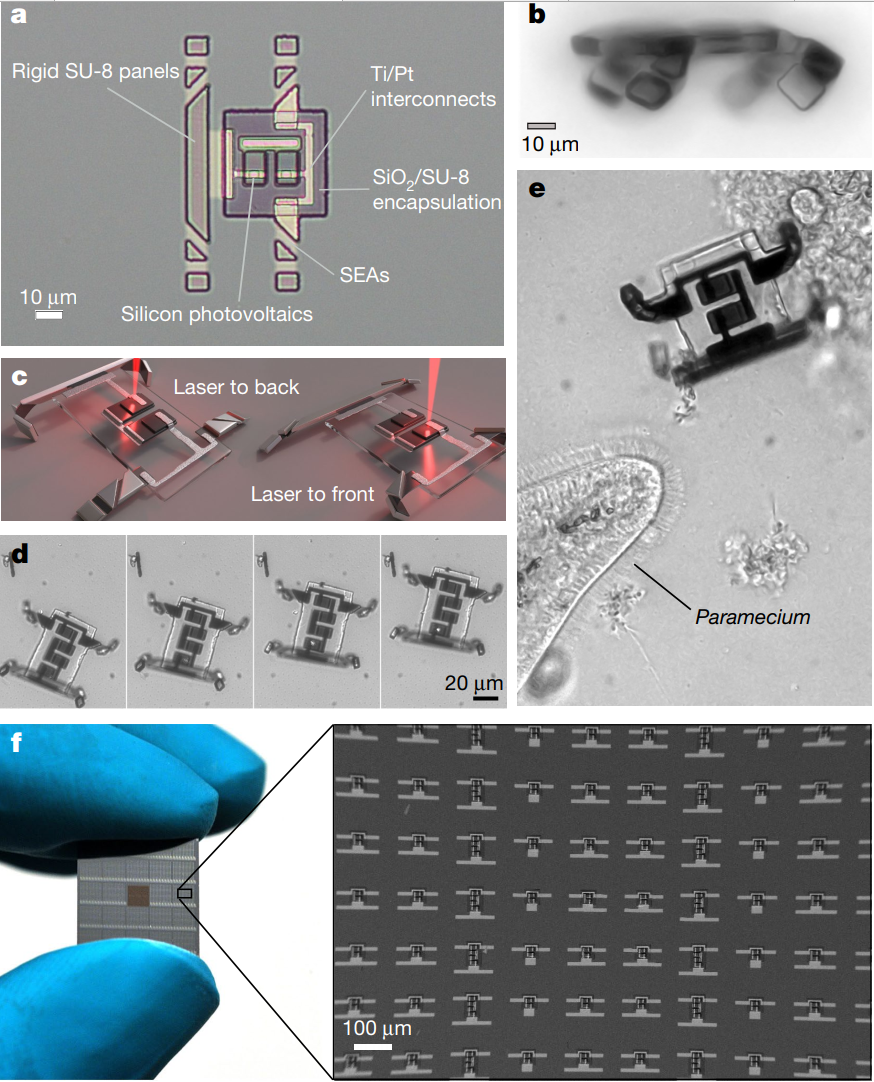
\includegraphics[width=.48\textwidth]{laser.PNG}
    \caption{Electronically integrated microscopic robots fabricated in parallel\cite{Miskin2020}.}
    \label{laser}
\end{figure}

\begin{figure}[htbp]
    \centering
    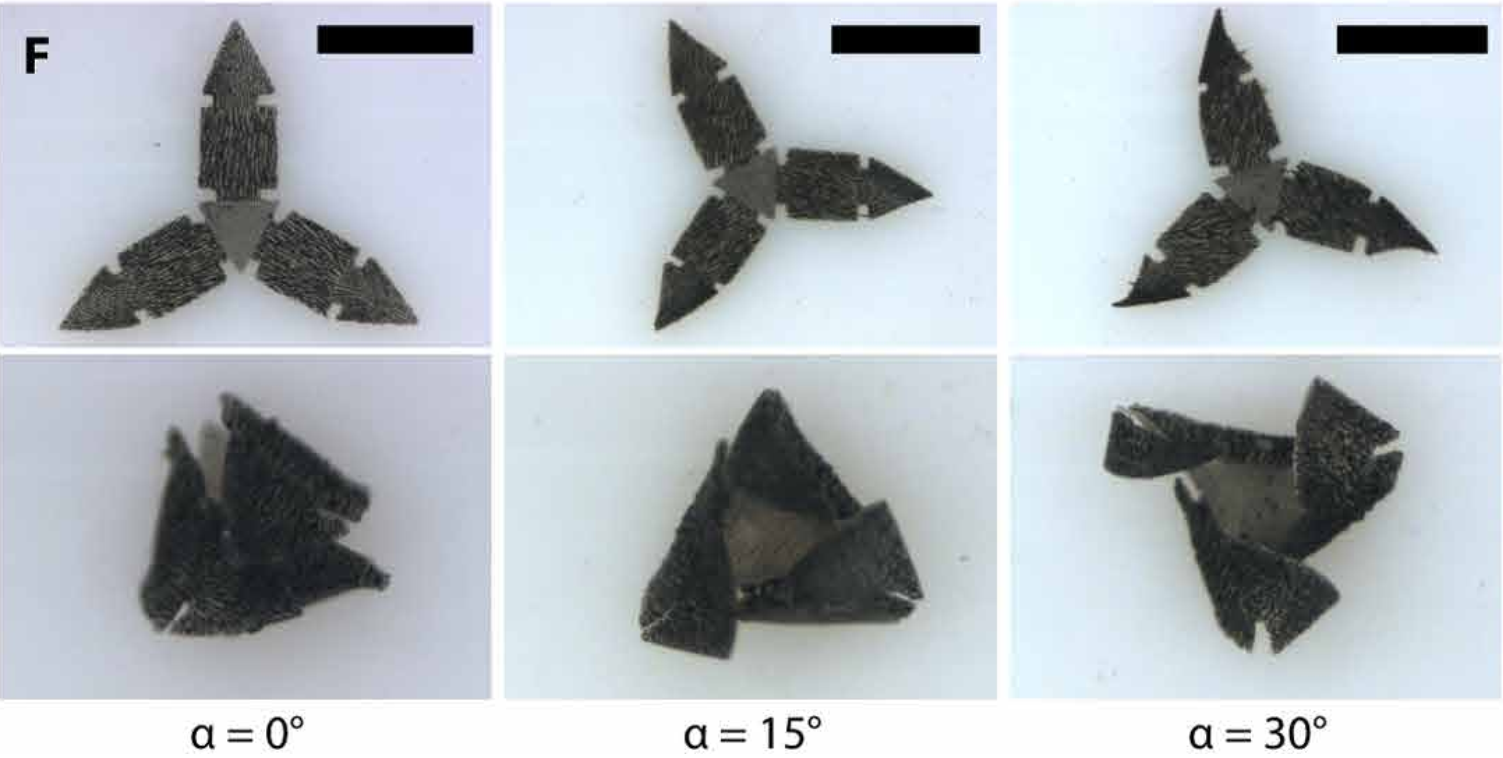
\includegraphics[width=.48\textwidth]{magnetic.PNG}
    \caption{Top view images of the tri-arm structures that bear different magnetization profiles. They were actuated under a 20-mT magnetic field out of the plane. Scale bars, 2 mm.\cite{Xu2019}.}
    \label{magnetic}
    \vspace{-0.8cm}
\end{figure}

Another approach for actuating is pumping. Many techniques have been developed to pump liquids in microfluidic devices, including micromechanical methods\cite{Stone2004}, electro-osmosis\cite{Manz1994}, ac thermocapillary pumping\cite{Kataoka1999}, electro-wetting\cite{Beni1981}, electrohydrodynamic pumping\cite{fuhr1992}, ac electro-osmosis\cite{Brown2000}, etc. In recent years, AC electro-osmosis (ACEO) has been considered a promising microfluidic mechanism that attracted increasing attention from researchers. ACEO is compatible with IC technology\cite{islam2006} and CMOS circuits. It can be fabricated with the CMOS process just as the other two approaches mentioned above. However, it can provide a long-lasting pumping speed with only a few volts (lower than 10V). In Studer’s experiment, the pumping speed reaches up to 500 \textmu m/s in a microfluidic channels with a driving signal in the 1–10 kHz range and an amplitude of only a few volts \cite{Studer2004}, which is more than 10 times larger than the speed generated by the SEAs microrobot. This experiment was based on a co-planar asymmetric electrode pair’s structure put forward by Brown in 2001\cite{Brown2000}. In Fig.\ref{Comparison}, it shows the comparison of the expected performances between different actuator approaches. However, in most instance, according to the existing researches, pumping is usually applied to transport liquid or particles but not driving the microrobot itself. The reason that we choose to ACEO technique is that it reaches most of the expected requirement of the microrobot functioning in the ocean (See Fig.\ref{Comparison}). Moreover, ACEO can deal with dangerous chemical environment and transport particles when pumping. It can be mass-produced, too.

\begin{figure*}[htpb]
    \centering
    \begin{tikzpicture}[
    level 1/.style={sibling distance = 40mm, level distance=23mm},
    edge from parent/.style = {black,thick, draw},
    edge from parent path = {(\tikzparentnode.south) -- (\tikzchildnode.north)} >=latex,node distance = 1.2cm, edge from parent fork down
    ]
% root of the the initial tree, level 1
    \node[root] {Required properties of Microrobots in the ocean}
% The first level, as children of the initial tree
    child {node[level-2] (c1) {Low working voltages and low power consumption}}
    child {node[level-2] (c2) {Ability to integrated with CMOS circuits}}
    child {node[level-2] (c3) {Ability to provide a high and stable speed}}
    child {node[level-2] (c4) {Wireless power transmission}};

% The second level, relatively positioned nodes
    \begin{scope}[every node/.style={level-3}, node distance = 15mm]
    \node [below of = c1] (c11) {ACEO Pump};
    \node [below of = c11] (c12) {SEAs microrobot};
    \node [below of = c12] (c13) {Magnetic controlled microrobot};

    \node [below of = c2] (c21) {ACEO Pump};
    \node [below of = c21] (c22) {SEAs microrobot};

    \node [below of = c3] (c31) {ACEO Pump};
    \node [below of = c31] (c32) {Other pumping approaches};

    \node [below of = c4] (c41) {ACEO Pump};
    \node [below of = c41] (c42) {SEAs microrobot};
    \node [below of = c42,text width=9.5em] (c43) {Laser/solar/magnetic driven microrobot};
    
    \end{scope}

% lines from each level 1 node to every one of its "children"
    \draw[very thick] (c1.south) -- (c11.north);
    \draw[very thick] (c11.south) -- (c12.north);
    \draw[very thick] (c12.south) -- (c13.north);
    
    \draw[very thick] (c2.south) -- (c21.north);
    \draw[very thick] (c21.south) -- (c22.north);
  
    \draw[very thick] (c3.south) -- (c31.north);
    \draw[very thick] (c31.south) -- (c32.north);
        
    \draw[very thick] (c4.south) -- (c41.north);
    \draw[very thick] (c41.south) -- (c42.north);
    \draw[very thick] (c42.south) -- (c43.north);
        
    \end{tikzpicture}
    \vspace*{3mm}
    \caption{Tree structure of the expected properties for microrobots in the ocean. Level 1 contains several basic properties, and the children refer to corresponding techniques that reach the expectations.}
    \label{Comparison}
\end{figure*}

Our group has been investigating the possibility of realizing a silicon-based life form based on this special asymmetric pumping system. In this article, we report a tunable and effective ACEO micropump which was fabricated with traditional lithography techniques on a glass substrate. We studied the performances of the pump by finding the dependencies of its pumping velocity with the applied voltage amplitude, frequencies, and electrolyte solution theoretically. Also, we predicted the motion of the microrobot on the surface of a 0.01M KCl solution (Potassium Chloride solution) by simulation with COMSOL Multiphysics$\rm^{TM}$. Finally, we experimentally observed that the microrobot could be pushed by the ACEO pump in the KCl solution. In the future, we look forward to measuring the pumping speed and integrating a wireless power transmission system on it to make it work independently.


%===============================================================================
\section{Theory}
Consider an array of asymmetric electrode pairs etched on the quartz substrate immersed in the KCl aqueous solution with conductivity $\sigma$. On the surface between the fluid and the electrode, there will be an electrical double layer that consists of two parallel layers of charge surrounding the electrodes. The double layer is composed of the inner Stern layer and the outer Gouy diffuse layer, shown as Fig.\ref{fig:edl}. It can be modeled by parallel capacitors with each capacitor a parallel-plate capacitor. On the other hand, we assume that the bulk water acts as parallel resistors. Consider a single pair of electrodes, when an AC voltage $V_+=+\frac{1}{2}V_0e^{i\omega t}$ applied on the larger electrode and $V_-=-\frac{1}{2}V_0e^{i\omega t}$ applied on the smaller electrode, the electric field lines can be approximate to semicircles ignoring horizontal component of the electric field on the surface of electrodes.

Denote the ratio of the larger electrode to the smaller ratio as $k$. Choose $x_1$ and $x_2$ so that the x coordinates of two endpoints of the larger electrode are $x_1\sqrt{k}$ and $x_2\sqrt{k}$ and those of the the smaller electrode are $x_1/\sqrt{k}$ and $x_2/\sqrt{k}$ respectively. Take an infinitesimal tube of the bulk water with one end's width of $\Delta x\sqrt{k}$ and the other end's width of $\Delta x/\sqrt{k}$. The theoretical model is shown in Fig.\ref{fig:math_model}.
\begin{figure}[H]
    \centering
    \begin{tikzpicture}
        \fill[color=Au] (0, 1.2) rectangle (5, 2);
        \foreach \n in {0.25,0.75,...,4.75} {
            \pic at (\n, 1.8) {negativecharge};
        }
        \foreach \p in {0.5,1.3,2.1,2.9,3.7,4.5} {  % Strangely, using {0.5,1.3,...,4.5} will not show the last node
            \pic at (\p, 2.2) {positivecharge};
        }
        \draw [dashed] (0, 2.45) -- (5, 2.45);
        \pic at (4, 3) {positivecharge};
        \pic at (1, 3.25) {positivecharge};
        \pic at (2.5, 3.75) {negativecharge};
        \pic at (4.25, 4) {positivecharge};
        \pic at (2.75, 4.5) {positivecharge};
        \pic at (0.5, 5) {negativecharge};
        \pic at (2.25, 5.25) {positivecharge};
        \pic at (3.5, 5.5) {negativecharge};
        % \pic at (1.5, 6) {negativecharge};
        % \pic at (4.25, 7) {negativecharge};
        % \pic at (2.25, 6.75) {positivecharge};
        \draw (5, 2) -- (5.5, 2);
        \draw (5, 2.45) -- (5.5, 2.45);
        \draw [Latex-Latex] (5.25, 2) -- (5.25, 2.45);
        \node (a) at (6.25, 2.2) {Stern layer};
        % \draw (5, 7.2) -- (5.5, 7.2);
        % \draw [Latex-Latex] (5.25, 2.45) -- (5.25, 7.2);
        \draw [Latex-] (5.25, 2.45) -- (5.25, 5.7);
        % \node (b) at (6.25, 4.825) {Diffuse layer};
        \node (b) at (6.25, 4.075) {Diffuse layer};
    \end{tikzpicture}
    \caption{The model of electric double layer (EDL).}
    \label{fig:edl}
\end{figure}
\vspace{-0.6cm}
\begin{figure}[H]
    \centering
    \begin{tikzpicture}[baseline=(current bounding box.north)]
      % Define coordinates
      % \def\Radius{2}
      \path
        (0, 0) coordinate (S0)
        (6, 0) coordinate (L0)
        % -- coordinate (M)
        % (M) +(60:\Radius) coordinate (C)
        % +(120:\Radius) coordinate (D)
        (0.1, 0) coordinate (S1)
        (5, 0) coordinate (L1)
        (0.2, 0) coordinate (S2)
        (4, 0) coordinate (L2)
        (0.3, 0) coordinate (S3)
        (3, 0) coordinate (L3)
        (0.4, 0) coordinate (S4)
        (2, 0) coordinate (L4)
        (0.5, 0) coordinate (S5)
        (1, 0) coordinate (L5)
        % (0.75, 0) coordinate (SC)
      ;
      % Draw electric field lines
      \draw
        (L0) arc(0:180:3)
        (L1) arc(0:180:2.45)
        (L2) arc(0:180:1.9)
        (L3) arc(0:180:1.35)
        (L4) arc(0:180:0.8)
        (L5) arc(0:180:0.25)
      ;
      % Draw axes
      \draw [-Stealth] (-1, -0.1) -- (7, -0.1);
      \draw [-Stealth] (0.5+1/22, -0.1) -- (0.5+1/22,4);
      % Draw reference lines
      \draw [dashed] (0, 0) -- (0, -0.5);
      \draw [dashed] (0.5, 0) -- (0.5, -0.5);
      \draw [dashed] (1, 0) -- (1, -1);
      \draw [dashed] (6, 0) -- (6, -1);
      \draw [-Latex] (-0.5, -0.5) -- (0.25, -0.1);
      \draw [-Latex] (-0.5, 0.15) -- (0, -0.05);
      \draw [-Latex] (-0.5, 0.5) -- (0, 0.05);
      \draw [-Latex] (5.12132, 2.12132) -- (5.5, 2.5);
      % Draw electrodes
      \fill[color=Au] (S0) rectangle (0.5, -0.08);
      \fill[color=Cr] (0, -0.08) rectangle (0.5, -0.1);
      \fill[color=Au] (L5) rectangle (6, -0.08);
      \fill[color=Cr] (1, -0.08) rectangle (6, -0.1);
      % Draw double layers
      \fill[color=Snow4] (0, 0) rectangle (0.5, 0.1);
      \fill[color=Snow4] (1, 0) rectangle (6, 0.1);
      % Draw bulk water
      \fill[color=Aquamarine3, semitransparent] (-0.5, 0.1) rectangle (6.5, 3.5);
      \fill[color=Aquamarine3, semitransparent] (-0.5, 0.1) rectangle (0, -0.1);
      \fill[color=Aquamarine3, semitransparent] (0.5, 0.1) rectangle (1, -0.1);
      \fill[color=Aquamarine3, semitransparent] (6, 0.1) rectangle (6.5, -0.1);
      % Draw glass substrate
      \fill[color=Glass, semitransparent] (-0.5, -0.1) rectangle (6.5, -1.5);
      % Annotations of coordinates
      \path[inner sep=0pt]
        (S0) node[below=1.5em] {\tiny{$\frac{x_2}{\sqrt{k}}$}}
        (L0) node[below=2.5em] {\tiny{$x_2\sqrt{k}$}}
        (S5) node[below=1.5em] {\tiny{$\frac{x_1}{\sqrt{k}}$}}
        (L5) node[below=2.5em] {\tiny{$x_1\sqrt{k}$}}
        % (C) node[above right=.2em] {$C$}
        % (D) node[above left=.2em] {$D$}
        (-0.5, -0.5) node[left] {\tiny{$-\frac{1}{2}V_0e^{i\omega t}$}}
        (3.5, 0) node[below=0.5em] {\tiny{$+\frac{1}{2}V_0e^{i\omega t}$}}
        (7, 0) node[above=0.5em] {$x$}
        (0.5+1/22,4) node[right=0.5em] {$y$}
        (0.5, 3.25) node[right=0.5em] {Bulk water}
        (3.5, 0) node[below=2.5em] {Glass substrate}
        (-0.5, 0.15) node[left] {\tiny{Au-Ge electrode}}
        (-0.5, 0.5) node[left] {\tiny{Double layer}}
        (5.5, 2.7) node[above right] {\tiny{Electric}}
        (5.5, 2.5) node[above right] {\tiny{field line}}
        (0.6, 0) node[below=0.5em] {\footnotesize{0}}
      ;
    \end{tikzpicture}
    \caption{An asymmetric electrode pair immersed in water \cite{physrevep}. The Au-Ge electrode consists of a layer of gold on the top and a layer of chromium on the bottom with thickness of 40\,nm and 5\,nm respectively.}
    \label{fig:math_model}
\end{figure}
\vspace{-0.3cm}
Using Debye-Huckel approximation, the characteristic thickness of the diffuse layer can be determined. The Debye length $\lambda_D$ is introduced as a scale for the decay of charge density. The two-dimensional capacitance at the larger electrode and the smaller electrode per unit length are respectively
\begin{equation}
    C_{DL}=\frac{\varepsilon\sqrt{k}\Delta x}{\lambda_D},
\end{equation}
\begin{equation}
    C_{DS}=\frac{\varepsilon\Delta x}{\sqrt{k}\lambda_D},
\end{equation}
where $\varepsilon=\varepsilon_r\varepsilon_0$ is the permittivity of the liquid \cite{physrevep}. For two dimensional model, the resistance $R(x)$ of the infinitesimal tube as a function of $x$ is given by
\begin{equation}
    R(x)=\frac{\pi(1+k)x}{2\sigma\sqrt{k}\Delta x}.
\end{equation}

where $\sigma$ is the conductivity of the fluid. The whole circuit equation is
\begin{equation}
    V_+-V_-=IR(x)+\Phi_L(x)+\Phi_S(x),
\end{equation}
where $I$ is the electric current flowing through the infinitesimal tube, and the potential drop on the double layer outside the larger electrode and that outside the smaller electrode are respectively
\begin{equation}
    \Phi_L(x)=\frac{I}{i\omega C_{LD}}
\end{equation}
\begin{equation}
    \Phi_S(x)=\frac{I}{i\omega C_{SD}}
\end{equation}

Solving the equations,
\begin{equation}
    \Phi_L(x)=\frac{V_0e^{i\omega t}}{(1+k)\left(1+\dfrac{i\omega\pi\varepsilon x}{2\sigma\lambda_D}\right)}.
\end{equation}

The component of the electric field in the $x$ direction on the larger electrode is then given by the derivative of the potential drop with respect to $x$,
\begin{equation}
    E_{xL}=\frac{\mathrm{d}\Phi_L(x)}{\mathrm{d}\left(x\sqrt{k}\right)}=-\frac{\dfrac{i\omega\pi\varepsilon V_0e^{i\omega t}}{2\sigma\lambda_D}}{\sqrt{k}(1+k)\left(1+\dfrac{i\omega\pi\varepsilon}{\sigma\lambda_D}\right)^2}.
\end{equation}

The liquid motion can be described by the Navier-Stokes equations for incompressible fluids
\begin{equation}
    \rho_m\frac{\mathrm{D}\mathbf{u}}{\mathrm{D}t}=-\nabla p+\rho_m\mathbf{g}+\mu\nabla^2\mathbf{u},
    \label{NS-Eq}
\end{equation}
\begin{equation}
    \nabla\cdot\mathbf{u}=0.
\end{equation}
Here $\rho_m$ denotes the mass density of the fluid, $\mathbf{u}$ is the fluid velocity, $p$ refers to the pressure, $g$ is body accelerations acting on the fluid, and $\mu$ represents the dynamic velocity of the fluid.

For AC electro-osmosis flow, the Reynolds number is sufficiently small so that a laminar flow assumption holds, and the inertia term can be neglected. The body force is provided by the electric field, so $\rho_m\mathbf{g}=\rho_e\mathbf{E}$, where $\rho_e$ is the volume charge density. The time average tangential velocity over the larger electrode is denoted as $u_{tL}$. Consider the time average form of Eq. \ref{NS-Eq} in the $x$ direction
\begin{equation}
    \mu\left(\frac{\partial^2u_{tL}}{\partial x^2}+\frac{\partial^2u_{tL}}{\partial y^2}\right)=\left<\rho_eE_{xL}\right>+\frac{\partial p}{\partial x},
\end{equation}
where $\left<\cdot\right>$ indicates the time average \cite{physreveii}. Since the derivative of $p$ with respect to $x$ is negligible and $u_{tL}$ does not have $y$ component, the equation becomes
\begin{equation}
    \mu\frac{\partial^2u_{tL}}{\partial y^2}=\left<\rho_eE_{xL}\right>
\end{equation}

\begin{figure}[htp]
    \centering
    \begin{tikzpicture}[circuit ee IEC,x=6cm,y=1cm,semithick,
                    every info/.style={font=\tiny},
                    small circuit symbols,
                    set resistor graphic=var resistor IEC graphic,
                    % set capacitor graphic=var capacitor IEC graphic,
                    set make contact graphic= var make contact IEC graphic]
        % Let us start with some contacts:
        \foreach \contact/\y in {1/1,2/2}
        {
            \node [contact] (left contact \contact) at (0,\y) {};
            \node [contact] (right contact \contact) at (1,\y) {};
        }
        \draw (left contact 1) -- (left contact 2);
        \draw (right contact 1) -- (right contact 2);
        \draw (left contact 1) to ++(down:1) to [ac source={info=$V_0e^{i\omega t}$}] ++(right:1) to (right contact 1);
        \draw (left contact 1) to [capacitor={near start, info={$C_{DS}(x_1)$}},resistor={info={$R(x_1)$}},capacitor={near end, info={$C_{DL}(x_1)$}}] (right contact 1);
        \draw (left contact 2) to [capacitor={near start, info={$C_{DS}(x_1+\Delta x)$}},resistor={info={$R(x_1+\Delta x)$}},capacitor={near end, info={$C_{DL}(x_1+\Delta x)$}}] (right contact 2);
        \draw (left contact 2) to ++(up:2) to [capacitor={near start, info={$C_{DS}(x_2)$}},resistor={info={$R(x_2)$},label={[label distance=0.75cm]south:\dots}},capacitor={near end, info={$C_{DL}(x_2)$}}] ++(right:1) to (right contact 2);
    \end{tikzpicture}
    \caption{The equivalent-circuit diagram of the theoretical model. Every row is a tube infinitesimal with the $x$ coordinate varies from $x_1$ to $x_2$.}
    \label{fig:2}
    \vspace{-0.63cm}
\end{figure}
Degrade to two-dimensional physics, integrate $u_{tL}$ from $y=0$ to $y=\lambda_D$, using $u_{tL}(y=0)=0$, the time average tangential velocity of the flow across the double layer on the larger electrode can be determined by
\begin{equation}
    u_{tL}=\frac{\lambda_D}{\mu}\left<\sigma_{eL}E_{xL}\right>,
\end{equation}
where the surface charge density determined by Gauss's law is
\begin{equation}
    \sigma_{eL}=\frac{\varepsilon\Phi_L}{\lambda_D}.
\end{equation}

For two harmonic functions $\sigma_{eL}$ and $E_{xL}$, the time average of their product is
\begin{equation}
    \begin{aligned}
        \left<\sigma_{eL}E_{xL}\right>&=\frac{1}{T}\int_0^T{\sigma_{e0}E_{xL0}\cos{(\omega t+\varphi_1)}\cos{(\omega t+\varphi_2)}\mathrm{d}t}\\
        &=\frac{1}{2}\sigma_{eL0}E_{xL0}\cos{(\varphi_1-\varphi_2)}\\
        &=\frac{1}{2}\mathrm{Re}\left(\sigma_{eL0}E_{xL0}e^{i\varphi_1}e^{-i\varphi_2}\right)\\
        &=\frac{1}{2}\mathrm{Re}\left(\sigma_{eL}E_{xL}^*\right)
    \end{aligned}
\end{equation}
Solving the equations,
\begin{equation}
    u_{tL}(x)=-\frac{\pi^2\varepsilon^3\omega^2V_0^2x}{8\sqrt{k}(1+k)\mu\sigma^2\left(1+\dfrac{\pi^2\varepsilon^2\omega^2x^2}{4\sigma^2\lambda_D^2}\right)^2\lambda_D^2}.
\end{equation}

The average velocity above the larger electrode is then
\newpage

\begin{strip}
    % The IEEE uses as a separator
    \rule{0.5\textwidth}{.4pt}
    \begin{equation}
        u_L=\frac{\int_{x_1\sqrt{k}}^{x_2\sqrt{k}}{u_{tL}(x)\mathrm{d}x}}{(x_2-x_1)\sqrt{k}}=-\frac{\pi^2\varepsilon^3\sigma^2\omega^2\lambda_D^2\left(x_2^2-x_1^2\right)V_0^2}{\sqrt{k}(1+k)^2\mu(x_2-x_1)\left(\pi^2\varepsilon^2\omega^2x_1^2+4\sigma^2\lambda_D^2\right)\left(\pi^2\varepsilon^2\omega^2x_2^2+4\sigma^2\lambda_D^2\right)},
    \end{equation}
    \hspace{0.5\textwidth}\rule{0.5\textwidth}{.4pt}
\end{strip}

and the average velocity above the smaller electrode $u_S$ is $-k^3$ times of $u_L$:
\begin{equation}
    u_S=-k^3u_L.
\end{equation}

The equivalent-circuit diagram of the theoretical model is shown in Fig. \ref{fig:2}.
Based on the diagram, the impedance of a tube infinitesimal can be calculated by
\begin{equation}
    Z(x)=R+\frac{1}{i\omega C_{DL}}+\frac{1}{i\omega C_{DS}}=\frac{(1+k)(\pi\varepsilon\omega x-2i\sigma\lambda_D)}{2\sqrt{k}\varepsilon\sigma\omega\Delta x}.
\end{equation}

Substitute $\mathrm{d}x$ for $\Delta x$, the total impedance is therefore

\begin{strip}
    \rule{0.5\textwidth}{.4pt}
    \begin{equation}
        Z_\text{total}=\frac{1}{\int_{x_1}^{x_2}{\dfrac{2\sqrt{k}\varepsilon\sigma\omega\mathrm{d}x}{(1+k)(\pi\varepsilon\omega x-2i\sigma\lambda_D)}}}=\frac{(1+k)\pi}{\sqrt{k}\sigma\left(2i\arctan{\left(\dfrac{2\pi\varepsilon\sigma\omega (x_2-x_1)\lambda_D}{\pi^2\varepsilon^2\omega^2x_1x_2+4\sigma^2\lambda_D^2}\right)}+\ln{\left(\dfrac{\pi^2\varepsilon^2\omega^2x_2^2+4\sigma^2\lambda_D^2}{\pi^2\varepsilon^2\omega^2x_1^2+4\sigma^2\lambda_D^2}\right)}\right)}
    \end{equation}
    \hspace{0.5\textwidth}\rule{0.5\textwidth}{.4pt}
\end{strip}


%===============================================================================
\section{Simulation}
\subsection{MATLAB}
\begin{figure}[htp]
    \centering

    \begin{tikzpicture}[baseline=(current bounding box.north)]
    \fill[color={Au}] (-0.5, 0) rectangle (0, 0.1);
    \fill[color={Au}] (0.5, 0) rectangle (2.5, 0.1);
    \fill[color={Au}] (4, 0) rectangle (4.5, 0.1);
    \fill[color={Au}] (5, 0) rectangle (7, 0.1);
    %axe
    \draw [->] (-1,0) -- (7.5,0) node[above=0.5em] {$x$};
    %line
    \draw [thick,>=latex,<->] (-0.5,-0.5) -- (0,-0.5);
    \draw [thick,>=latex,<->] (0,-0.5) -- (0.5,-0.5);
    \draw [thick,>=latex,<->] (0.5,-0.5) -- (2.5,-0.5);
    \draw [thick,>=latex,<->] (2.5,-0.5) -- (4,-0.5);
    
    \draw [dashed] (-0.5, 0) -- (-0.5, -0.5);
    \draw [dashed] (0, 0) -- (0, -0.5);
    \draw [dashed] (0.5, 0) -- (0.5, -0.5);
    \draw [dashed] (2.5, 0) -- (2.5, -0.5);
    \draw [dashed] (4, 0) -- (4, -0.5);
    %label
    \path[inner sep=0pt]
        (-0.25, 0) node[below=2em] {$S$}
        (0.25, 0) node[below=2em] {$G$}
        (1.5, 0) node[below=2em] {$L$}
        (3.25, 0) node[below=2em] {$G_{1}$};
    \end{tikzpicture}
    \caption{Coordinate system used for the computation of the average velocity.}
    \label{simplified}
\end{figure}

\vspace{-0.63cm}
According to Brown \textit{et al.}\cite{Brown2000}, given the geometry of the system shown as Fig.\ref{fig:math_model}. Here we give a simplified representation of each component in this system shown as Fig.\ref{simplified}, where for given width-ratio $k = L/S$ of the electrodes. By substituting $\omega_{0}$ and $v_{0}$ into Equation 17, we can get a simplified equation for the average velocity.
\begin{equation}
    u_{\textit{L}}=\frac{1}{x_{\max }-x_{\min }} \int_{x_{\min }}^{x_{\max }} \frac{v_{0}}{x} V_{0}^{2} \frac{\left(\omega x / \omega_{0}\right)^{2}}{\left(1+\left(\omega x / \omega_{0}\right)^{2}\right)^{2}} \mathrm{~d} x,
\end{equation}
where $v_{0}$ is
\begin{equation}
    v_{0}=\frac{\epsilon}{2 \eta \sqrt{k}(1+k)^{2}}
\end{equation}
and $\omega_{0}$ is
\begin{equation}
    \omega_{0}=\frac{2 \sigma_{0} \lambda_{D}}{\pi \epsilon}
\end{equation}

\begin{figure*}[ht]
	\centering
	\subfloat[Different ratios of electrodes.]{% This file was created by matlab2tikz.
%
%The latest updates can be retrieved from
%  http://www.mathworks.com/matlabcentral/fileexchange/22022-matlab2tikz-matlab2tikz
%where you can also make suggestions and rate matlab2tikz.
%
\definecolor{mycolor1}{rgb}{0.00000,0.44700,0.74100}%
\definecolor{mycolor2}{rgb}{0.85000,0.32500,0.09800}%
\definecolor{mycolor3}{rgb}{0.92900,0.69400,0.12500}%
\definecolor{mycolor4}{rgb}{0.49400,0.18400,0.55600}%
%
\begin{tikzpicture}[scale=0.65]

\begin{axis}[%
thick,
width=4.521in,
height=3.559in,
at={(0.758in,0.488in)},
scale only axis,
xmode=log,
xmin=10,
xmax=100000,
xminorticks=true,
xlabel style={font=\color{white!15!black}},
xlabel={Frequency / Hz},
ymin=0,
ymax=160,
ylabel style={font=\color{white!15!black}},
ylabel={$\text{Simulated x-velocity / }\mu\text{m/s}$},
axis background/.style={fill=white},
title={Velocity vs. Frequency \& electrodes dimensions (1.5V)},
legend style={at={(0.03,0.97)}, anchor=north west, legend cell align=left, align=left, draw=white!15!black}
]
\addplot [color=mycolor1,very thick]
  table[row sep=crcr]{%
10	0.431600164133989\\
10.9749876549306	0.517732503857856\\
12.0450354025878	0.620545076946781\\
13.2194114846603	0.743047260742358\\
14.5082877849594	0.888696476664339\\
15.9228279334109	1.061423898082\\
17.4752840000768	1.2656420767488\\
19.1791026167249	1.50622429043277\\
21.0490414451202	1.78844269927636\\
23.1012970008316	2.11784993936373\\
25.3536449397011	2.50008731861847\\
27.8255940220712	2.94060342467114\\
30.5385550883342	3.4442711598037\\
33.5160265093884	4.01490056146537\\
36.7837977182863	4.65466044631417\\
40.3701725859655	5.36344392135132\\
44.3062145758388	6.13823889358956\\
48.6260158006535	6.97258959609809\\
53.3669923120631	7.8562506332643\\
58.5702081805667	8.77513180971457\\
64.2807311728432	9.71160324899565\\
70.5480231071865	10.6451762222754\\
77.4263682681127	11.5535057973233\\
84.9753435908644	12.4135956658628\\
93.260334688322	13.2030445121557\\
102.353102189903	13.9011716917887\\
112.332403297803	14.4898989416469\\
123.284673944207	14.954331179948\\
135.304777457981	15.2830515204408\\
148.496826225447	15.4682021739041\\
162.975083462064	15.5054503223526\\
178.864952905744	15.3939329763577\\
196.304065004027	15.1362426325241\\
215.443469003188	14.738466941214\\
236.448941264541	14.2102436084147\\
259.502421139974	13.5647498141752\\
284.80358684358	12.8185257075325\\
312.571584968824	11.9910425078587\\
343.046928631492	11.1039687866364\\
376.493580679247	10.1801551105709\\
413.201240011533	9.24242932061254\\
453.487850812858	8.31234974041369\\
497.702356433211	7.40908310697164\\
546.227721768434	6.54855163212656\\
599.484250318941	5.74293777850018\\
657.933224657568	5.00056510560606\\
722.080901838546	4.32610994733189\\
792.482898353917	3.72105664604437\\
869.749002617783	3.18429358247619\\
954.548456661835	2.71275447428996\\
1047.61575278967	2.3020307619292\\
1149.75699539774	1.94690724962839\\
1261.85688306602	1.64179767483693\\
1384.88637139387	1.38107583864819\\
1519.91108295293	1.15931034426071\\
1668.10053720006	0.971417575995407\\
1830.73828029537	0.812749779153098\\
2009.23300256505	0.679134528934776\\
2205.13073990305	0.56687980046629\\
2420.12826479438	0.472756193940013\\
2656.08778294669	0.393965202064781\\
2915.05306282518	0.328100035078039\\
3199.26713779738	0.273103563355857\\
3511.19173421513	0.227226412250348\\
3853.52859371053	0.188987105066068\\
4229.2428743895	0.157135332419061\\
4641.58883361278	0.130618860847802\\
5094.13801481638	0.108554218325081\\
5590.81018251222	0.0902010575466567\\
6135.90727341318	0.0749399587994951\\
6734.15065775082	0.0622533619847647\\
7390.72203352578	0.0517092893519408\\
8111.30830789687	0.0429475205287326\\
8902.15085445038	0.0356678982560311\\
9770.09957299226	0.0296204692233297\\
10722.6722201032	0.0245971945135648\\
11768.11952435	0.0204249952013864\\
12915.4966501488	0.0169599286600805\\
14174.741629268	0.0140823190241676\\
15556.7614393047	0.0116926904909656\\
17073.5264747069	0.00970837454623428\\
18738.1742286039	0.0080606818065599\\
20565.1230834865	0.0066925461507238\\
22570.1971963392	0.00555656339541084\\
24770.7635599171	0.00461335921482758\\
27185.8824273294	0.00383023156855065\\
29836.4724028334	0.00318002183441078\\
32745.4916287773	0.00264017637073972\\
35938.1366380463	0.00219196655891431\\
39442.0605943766	0.00181984068286876\\
43287.6128108306	0.00151088544394497\\
47508.1016210279	0.00125437862241823\\
52140.0828799968	0.0010414174971286\\
57223.6765935022	0.000864610220489003\\
62802.9144183425	0.000717819501291315\\
68926.121043497	0.000595949742727411\\
75646.3327554629	0.000494770277246015\\
83021.7568131974	0.000410768583116206\\
91116.2756115491	0.000341028401622686\\
100000	0.000283128533608519\\
};
\addlegendentry{$\text{50-30-20}\mu\text{m}$}

\addplot [color=mycolor2,very thick]
  table[row sep=crcr]{%
10	0.219105788217367\\
10.9749876549306	0.263638546618404\\
12.0450354025878	0.317155248149621\\
13.2194114846603	0.381438269236744\\
14.5082877849594	0.458610233518519\\
15.9228279334109	0.551193012831626\\
17.4752840000768	0.662174281427821\\
19.1791026167249	0.795081318272841\\
21.0490414451202	0.954060985637599\\
23.1012970008316	1.14396365955798\\
25.3536449397011	1.37042722392471\\
27.8255940220712	1.63995492718177\\
30.5385550883342	1.9599778087039\\
33.5160265093884	2.3388884483432\\
36.7837977182863	2.78602801151716\\
40.3701725859655	3.31160321145423\\
44.3062145758388	3.92650451958838\\
48.6260158006535	4.64199290193674\\
53.3669923120631	5.46922142543704\\
58.5702081805667	6.41856288929974\\
64.2807311728432	7.49872832088117\\
70.5480231071865	8.71568663810554\\
77.4263682681127	10.0714343319936\\
84.9753435908644	11.5627134413758\\
93.260334688322	13.1798286672836\\
102.353102189903	14.9057562184191\\
112.332403297803	16.7157495622928\\
123.284673944207	18.5776137200662\\
135.304777457981	20.4527331348687\\
148.496826225447	22.2978094474541\\
162.975083462064	24.0671254513725\\
178.864952905744	25.7150423753387\\
196.304065004027	27.1983968503999\\
215.443469003188	28.4785069749944\\
236.448941264541	29.5226096276029\\
259.502421139974	30.3046958708587\\
284.80358684358	30.8058428908265\\
312.571584968824	31.0142240557311\\
343.046928631492	30.9249973718716\\
376.493580679247	30.540230486452\\
413.201240011533	29.8689349016304\\
453.487850812858	28.9271777891398\\
497.702356433211	27.7381436116946\\
546.227721768434	26.3319556103647\\
599.484250318941	24.7450601467703\\
657.933224657568	23.0190349208656\\
722.080901838546	21.1987975219183\\
792.482898353917	19.3303354101352\\
869.749002617783	17.4582093407406\\
954.548456661835	15.6231565466331\\
1047.61575278967	13.8601126031811\\
1149.75699539774	12.1968855916926\\
1261.85688306602	10.6535832948837\\
1384.88637139387	9.2427562684912\\
1519.91108295293	7.97011366243247\\
1668.10053720006	6.83561381218508\\
1830.73828029537	5.83472739399131\\
2009.23300256505	4.95970328130729\\
2205.13073990305	4.200717477147\\
2420.12826479438	3.54683746387904\\
2656.08778294669	2.98677775796728\\
2915.05306282518	2.50945316176615\\
3199.26713779738	2.1043543147324\\
3511.19173421513	1.76177812997548\\
3853.52859371053	1.47294671887781\\
4229.2428743895	1.23004533530714\\
4641.58883361278	1.02620489851345\\
5094.13801481638	0.855449224864789\\
5590.81018251222	0.71262204092342\\
6135.90727341318	0.593304551123129\\
6734.15065775082	0.493730901140548\\
7390.72203352578	0.410706266948153\\
8111.30830789687	0.341530392216349\\
8902.15085445038	0.283928055126008\\
9770.09957299226	0.235987038013948\\
10722.6722201032	0.19610358636179\\
11768.11952435	0.16293498621755\\
12915.4966501488	0.135358690961962\\
14174.741629268	0.112437337160131\\
15556.7614393047	0.0933889673322349\\
17073.5264747069	0.0775617982624073\\
18738.1742286039	0.0644129186993548\\
20565.1230834865	0.0534903577926128\\
22570.1971963392	0.044418027458337\\
24770.7635599171	0.0368831031705268\\
27185.8824273294	0.0306254655552733\\
29836.4724028334	0.0254288781101507\\
32745.4916287773	0.0211136237394092\\
35938.1366380463	0.0175303644987981\\
39442.0605943766	0.0145550252190339\\
43287.6128108306	0.0120845329402974\\
47508.1016210279	0.0100332708408368\\
52140.0828799968	0.00833012810249191\\
57223.6765935022	0.00691604643268975\\
62802.9144183425	0.00574198022997205\\
68926.121043497	0.00476720106790855\\
75646.3327554629	0.00395788866197047\\
83021.7568131974	0.00328596010984042\\
91116.2756115491	0.00272809724724028\\
100000	0.00226493868736114\\
};
\addlegendentry{$\text{25-15-10}\mu\text{m}$}

\addplot [color=mycolor3,very thick]
  table[row sep=crcr]{%
10	0.0880195692928828\\
10.9749876549306	0.106002111918455\\
12.0450354025878	0.127654145710275\\
13.2194114846603	0.153722493709344\\
14.5082877849594	0.18510508863433\\
15.9228279334109	0.222881149586307\\
17.4752840000768	0.268347205636524\\
19.1791026167249	0.323060017878702\\
21.0490414451202	0.38888760316056\\
23.1012970008316	0.468069717908513\\
25.3536449397011	0.563289308421232\\
27.8255940220712	0.677756557127788\\
30.5385550883342	0.815307225151246\\
33.5160265093884	0.980516968742713\\
36.7837977182863	1.17883313014081\\
40.3701725859655	1.41672508553529\\
44.3062145758388	1.70185345336416\\
48.6260158006535	2.04325716158504\\
53.3669923120631	2.45155532837823\\
58.5702081805667	2.93915785737677\\
64.2807311728432	3.52047426639707\\
70.5480231071865	4.21210421195958\\
77.4263682681127	5.03298512530572\\
84.9753435908644	6.0044621636307\\
93.260334688322	7.15023345293965\\
102.353102189903	8.49611011531439\\
112.332403297803	10.0695175857091\\
123.284673944207	11.8986554194569\\
135.304777457981	14.0112321623371\\
148.496826225447	16.4327067166639\\
162.975083462064	19.1840058790487\\
178.864952905744	22.2787562694291\\
196.304065004027	25.7201699952782\\
215.443469003188	29.4978497558366\\
236.448941264541	33.584909047794\\
259.502421139974	37.9358995491564\\
284.80358684358	42.4860541750895\\
312.571584968824	47.1522506200605\\
343.046928631492	51.8358647615709\\
376.493580679247	56.4273512748989\\
413.201240011533	60.8120433215903\\
453.487850812858	64.8764110881883\\
497.702356433211	68.5139479065741\\
546.227721768434	71.6299906873751\\
599.484250318941	74.1450823281233\\
657.933224657568	75.9968476026642\\
722.080901838546	77.1406693759077\\
792.482898353917	77.5496367722852\\
869.749002617783	77.2142590673246\\
954.548456661835	76.1423139753985\\
1047.61575278967	74.3589740148265\\
1149.75699539774	71.9070926621272\\
1261.85688306602	68.8473004044005\\
1384.88637139387	65.2574233269256\\
1519.91108295293	61.2307430795995\\
1668.10053720006	56.8727863119999\\
1830.73828029537	52.2966369943476\\
2009.23300256505	47.617128843788\\
2205.13073990305	42.9445872511399\\
2420.12826479438	38.3789474440493\\
2656.08778294669	34.0050252482454\\
2915.05306282518	29.8894794582308\\
3199.26713779738	26.0796637732411\\
3511.19173421513	22.6042285259194\\
3853.52859371053	19.4750850023326\\
4229.2428743895	16.6902282838483\\
4641.58883361278	14.2369205668398\\
5094.13801481638	12.0948275287503\\
5590.81018251222	10.2388288307637\\
6135.90727341318	8.64135179208846\\
6734.15065775082	7.27418142537088\\
7390.72203352578	6.10977180821007\\
8111.30830789687	5.12212474251036\\
8902.15085445038	4.28731847384303\\
9770.09957299226	3.58376981717015\\
10722.6722201032	2.99230433649382\\
11768.11952435	2.49609643376519\\
12915.4966501488	2.08052766972069\\
14174.741629268	1.73299924074141\\
15556.7614393047	1.44272411011315\\
17073.5264747069	1.2005160352305\\
18738.1742286039	0.998586491341809\\
20565.1230834865	0.830355959946346\\
22570.1971963392	0.690282879928142\\
24770.7635599171	0.57371142829374\\
27185.8824273294	0.476737929989422\\
29836.4724028334	0.396094872881132\\
32745.4916287773	0.329051056306523\\
35938.1366380463	0.273326205095885\\
39442.0605943766	0.227018345978307\\
43287.6128108306	0.188542306974767\\
47508.1016210279	0.156577819737832\\
52140.0828799968	0.130025851218282\\
57223.6765935022	0.107971946095182\\
62802.9144183425	0.0896555137301669\\
68926.121043497	0.0744441364251031\\
75646.3327554629	0.0618121060795629\\
83021.7568131974	0.0513225126164221\\
91116.2756115491	0.0426123097004962\\
100000	0.0353798719973139\\
};
\addlegendentry{$\text{10-6-4}\mu\text{m}$}

\addplot [color=mycolor4,very thick]
  table[row sep=crcr]{%
10	0.0440368590728688\\
10.9749876549306	0.0530403283898138\\
12.0450354025878	0.0638840365811292\\
13.2194114846603	0.0769438672813812\\
14.5082877849594	0.0926723701665603\\
15.9228279334109	0.111614347810466\\
17.4752840000768	0.134425588892703\\
19.1791026167249	0.161895372683868\\
21.0490414451202	0.194973489235933\\
23.1012970008316	0.234802659943456\\
25.3536449397011	0.28275740671241\\
27.8255940220712	0.340490607288078\\
30.5385550883342	0.409989191224968\\
33.5160265093884	0.493640676319752\\
36.7837977182863	0.594312517940601\\
40.3701725859655	0.715446539265821\\
44.3062145758388	0.861171019667625\\
48.6260158006535	1.03643332434585\\
53.3669923120631	1.24715623239001\\
58.5702081805667	1.50042131758958\\
64.2807311728432	1.80468278752983\\
70.5480231071865	2.17001498943807\\
77.4263682681127	2.6083961979123\\
84.9753435908644	3.13403010148862\\
93.260334688322	3.76370431564416\\
102.353102189903	4.51718188792213\\
112.332403297803	5.41761663709057\\
123.284673944207	6.49197568537617\\
135.304777457981	7.77144202356474\\
148.496826225447	9.29175571528489\\
162.975083462064	11.0934338863878\\
178.864952905744	13.2217869071212\\
196.304065004027	15.726622044518\\
215.443469003188	18.6614988435223\\
236.448941264541	22.082377561128\\
259.502421139974	26.0454914221622\\
284.80358684358	30.6042873464213\\
312.571584968824	35.80533325453\\
343.046928631492	41.6831985172183\\
376.493580679247	48.2544874261089\\
413.201240011533	55.5114390219514\\
453.487850812858	63.4157707109758\\
497.702356433211	71.8936770445706\\
546.227721768434	80.833011578881\\
599.484250318941	90.0835879333052\\
657.933224657568	99.4611814731226\\
722.080901838546	108.755220647294\\
792.482898353917	117.739452838705\\
869.749002617783	126.184255078131\\
954.548456661835	133.868939251482\\
1047.61575278967	140.592491800311\\
1149.75699539774	146.18166296206\\
1261.85688306602	150.496019987302\\
1384.88637139387	153.430278499496\\
1519.91108295293	154.914727636386\\
1668.10053720006	154.914756749014\\
1830.73828029537	153.430365163167\\
2009.23300256505	150.496162168065\\
2205.13073990305	146.181857242625\\
2420.12826479438	140.592733372566\\
2656.08778294669	133.869221963973\\
2915.05306282518	126.184571576289\\
3199.26713779738	117.739794821685\\
3511.19173421513	108.755579240766\\
3853.52859371053	99.4615476885231\\
4229.2428743895	90.083953159761\\
4641.58883361278	80.8333680422891\\
5094.13801481638	71.8940181731548\\
5590.81018251222	63.416091366067\\
6135.90727341318	55.5117355799371\\
6734.15065775082	48.2547577239666\\
7390.72203352578	41.6834416930354\\
8111.30830789687	35.8055495229946\\
8902.15085445038	30.6044777482473\\
9770.09957299226	26.0456575789455\\
10722.6722201032	22.0825214568986\\
11768.11952435	18.6616226442485\\
12915.4966501488	15.7267279587728\\
14174.741629268	13.2218770856451\\
15556.7614393047	11.093510355213\\
17073.5264747069	9.29182033587295\\
18738.1742286039	7.7714964734381\\
20565.1230834865	6.49202145344175\\
22570.1971963392	5.41765502887293\\
24770.7635599171	4.51721403698572\\
27185.8824273294	3.76373119844793\\
29836.4724028334	3.13405255372329\\
32745.4916287773	2.60841493100775\\
35938.1366380463	2.17003060640672\\
39442.0605943766	1.80469579765963\\
43287.6128108306	1.50043214974225\\
47508.1016210279	1.24716524682218\\
52140.0828799968	1.03644082307459\\
57223.6765935022	0.861177255463927\\
62802.9144183425	0.715451723392984\\
68926.121043497	0.594316826768672\\
75646.3327554629	0.493644256949435\\
83021.7568131974	0.409992166248832\\
91116.2756115491	0.340493078807404\\
100000	0.282759459716493\\
};
\addlegendentry{$\text{5-3-2}\mu\text{m}$}

\node[right, align=left]
at (axis cs:20,100) {$\text{c}_\text{0}\text{ = 0.01mM}$};
\end{axis}
\end{tikzpicture}%}
	\hspace{0.3in}
	\subfloat[Different ratios of electrodes, but with the same small electrode size]{% This file was created by matlab2tikz.
%
%The latest updates can be retrieved from
%  http://www.mathworks.com/matlabcentral/fileexchange/22022-matlab2tikz-matlab2tikz
%where you can also make suggestions and rate matlab2tikz.
%
\definecolor{mycolor1}{RGB}{41, 128, 185}%
\definecolor{mycolor2}{RGB}{211, 84, 0}%
\definecolor{mycolor3}{RGB}{241, 196, 15}%
\definecolor{mycolor4}{RGB}{142, 68, 173}%
%
\begin{tikzpicture}[scale=0.65]

\begin{axis}[%
thick,
width=4.521in,
height=3.559in,
at={(0.758in,0.488in)},
scale only axis,
xmode=log,
xmin=10,
xmax=100000,
xminorticks=true,
xlabel style={font=\color{white!15!black}},
xlabel={Frequency / Hz},
ymin=0,
ymax=60,
ylabel style={font=\color{white!15!black}},
ylabel={$\text{Simulated x-velocity / }\mu\text{m/s}$},
axis background/.style={fill=white},
title={Velocity vs. Frequency \& electrodes dimensions (1.5V)},
legend style={at={(0.03,0.97)}, anchor=north west, legend cell align=left, align=left, draw=white!15!black}
]
\addplot [color=mycolor1, very thick]
  table[row sep=crcr]{%
10	0.0183867331479636\\
10.9749876549306	0.0221402801886409\\
12.0450354025878	0.0266584693461776\\
13.2194114846603	0.0320963375881225\\
14.5082877849594	0.0386400290396865\\
15.9228279334109	0.0465128892579316\\
17.4752840000768	0.0559826872130859\\
19.1791026167249	0.0673701435279773\\
21.0490414451202	0.0810589575920205\\
23.1012970008316	0.0975075337339927\\
25.3536449397011	0.117262602689569\\
27.8255940220712	0.140974911804994\\
30.5385550883342	0.169417105340929\\
33.5160265093884	0.203503820403328\\
36.7837977182863	0.244313864919694\\
40.3701725859655	0.293114096295011\\
44.3062145758388	0.351384251294809\\
48.6260158006535	0.420841452358534\\
53.3669923120631	0.503462393938645\\
58.5702081805667	0.601500260916653\\
64.2807311728432	0.717492235170843\\
70.5480231071865	0.8542520336398\\
77.4263682681127	1.01484039590868\\
84.9753435908644	1.20250502735522\\
93.260334688322	1.4205806026131\\
102.353102189903	1.67233964885433\\
112.332403297803	1.96078726139732\\
123.284673944207	2.28839754446937\\
135.304777457981	2.65679812686641\\
148.496826225447	3.06642115343054\\
162.975083462064	3.51615366866135\\
178.864952905744	4.00303446801636\\
196.304065004027	4.52205378380779\\
215.443469003188	5.06611130221435\\
236.448941264541	5.62617287129651\\
259.502421139974	6.191636468272\\
284.80358684358	6.75087868406737\\
312.571584968824	7.29191440448257\\
343.046928631492	7.80307661638898\\
376.493580679247	8.273619292807\\
413.201240011533	8.69416579541402\\
453.487850812858	9.05696178884103\\
497.702356433211	9.3559338227336\\
546.227721768434	9.58659091879062\\
599.484250318941	9.74582913251233\\
657.933224657568	9.83170608924345\\
722.080901838546	9.84324625412285\\
792.482898353917	9.78032249482125\\
869.749002617783	9.64363944605511\\
954.548456661835	9.43482214476089\\
1047.61575278967	9.1565911357038\\
1149.75699539774	8.81298433937953\\
1261.85688306602	8.40956888210402\\
1384.88637139387	7.95357658779825\\
1519.91108295293	7.45389935986447\\
1668.10053720006	6.92089845720002\\
1830.73828029537	6.36601420826189\\
2009.23300256505	5.80120412945501\\
2205.13073990305	5.23827703792813\\
2420.12826479438	4.68821652685642\\
2656.08778294669	4.16059067870921\\
2915.05306282518	3.66312520767197\\
3199.26713779738	3.20148136686088\\
3511.19173421513	2.7792396020365\\
3853.52859371053	2.39805637266535\\
4229.2428743895	2.05794169180806\\
4641.58883361278	1.75759996380239\\
5094.13801481638	1.49478340165394\\
5590.81018251222	1.2666205047178\\
6135.90727341318	1.06989686942171\\
6734.15065775082	0.901278612592055\\
7390.72203352578	0.757478293016042\\
8111.30830789687	0.635369189138512\\
8902.15085445038	0.532056699439721\\
9770.09957299226	0.444916347555751\\
10722.6722201032	0.371607243708664\\
11768.11952435	0.310068548440789\\
12915.4966501488	0.258504963233364\\
14174.741629268	0.215365809162217\\
15556.7614393047	0.179320985913201\\
17073.5264747069	0.149236076385774\\
18738.1742286039	0.124148072360997\\
20565.1230834865	0.103242614712059\\
22570.1971963392	0.0858332289970117\\
24770.7635599171	0.071342755903322\\
27185.8824273294	0.0592869924558359\\
29836.4724028334	0.049260446818385\\
32745.4916287773	0.0409240456556129\\
35938.1366380463	0.0339946024448491\\
39442.0605943766	0.0282358462556158\\
43287.6128108306	0.0234508151467649\\
47508.1016210279	0.0194754308093893\\
52140.0828799968	0.016173087605006\\
57223.6765935022	0.0134301072353522\\
62802.9144183425	0.0111519283803175\\
68926.121043497	0.00925991783497766\\
75646.3327554629	0.00768870546971364\\
83021.7568131974	0.00638395950913841\\
91116.2756115491	0.00530053112984973\\
100000	0.00440090827205102\\
};
\addlegendentry{$\text{25-5-5}\mu\text{m}$}

\addplot [color=mycolor2,very thick]
  table[row sep=crcr]{%
10	0.0259529425189388\\
10.9749876549306	0.031252461378158\\
12.0450354025878	0.0376321729164238\\
13.2194114846603	0.045311372130439\\
14.5082877849594	0.0545534790822606\\
15.9228279334109	0.0656747399446588\\
17.4752840000768	0.0790545638973741\\
19.1791026167249	0.0951477671281998\\
21.0490414451202	0.114499023188469\\
23.1012970008316	0.137759841056017\\
25.3536449397011	0.165708402584366\\
27.8255940220712	0.199272580761017\\
30.5385550883342	0.239556416543479\\
33.5160265093884	0.28787023679701\\
36.7837977182863	0.34576442386727\\
40.3701725859655	0.415066564799605\\
44.3062145758388	0.497921271364832\\
48.6260158006535	0.596831316648807\\
53.3669923120631	0.714697817187804\\
58.5702081805667	0.854855936129807\\
64.2807311728432	1.02110093812987\\
70.5480231071865	1.21769737156416\\
77.4263682681127	1.4493617450495\\
84.9753435908644	1.72120649575092\\
93.260334688322	2.03863072241438\\
102.353102189903	2.40714177872879\\
112.332403297803	2.83209244743368\\
123.284673944207	3.31832241901891\\
135.304777457981	3.86970167119184\\
148.496826225447	4.48858821136495\\
162.975083462064	5.17523347487643\\
178.864952905744	5.9271933094378\\
196.304065004027	6.7388258758094\\
215.443469003188	7.60097214802889\\
236.448941264541	8.50091114829341\\
259.502421139974	9.42265417043032\\
284.80358684358	10.3475902604237\\
312.571584968824	11.2554287815398\\
343.046928631492	12.1253218779812\\
376.493580679247	12.9370102390083\\
413.201240011533	13.6718337432877\\
453.487850812858	14.3134856150656\\
497.702356433211	14.8484525438058\\
546.227721768434	15.2661538479034\\
599.484250318941	15.5588507629963\\
657.933224657568	15.7214299866654\\
722.080901838546	15.7511706009505\\
792.482898353917	15.6475844768216\\
869.749002617783	15.4123847063765\\
954.548456661835	15.0495923691028\\
1047.61575278967	14.5657461692986\\
1149.75699539774	13.9701391234888\\
1261.85688306602	13.2749790929601\\
1384.88637139387	12.495363456536\\
1519.91108295293	11.6489786430759\\
1668.10053720006	10.7554830924284\\
1830.73828029537	9.83559929948705\\
2009.23300256505	8.91001007857158\\
2205.13073990305	7.99820531117019\\
2420.12826479438	7.11744164188624\\
2656.08778294669	6.28195385677131\\
2915.05306282518	5.50250186009195\\
3199.26713779738	4.78626972218816\\
3511.19173421513	4.13707307832877\\
3853.52859371053	3.55579197662883\\
4229.2428743895	3.04093237427285\\
4641.58883361278	2.58922690416948\\
5094.13801481638	2.19620599032868\\
5590.81018251222	1.85669528194773\\
6135.90727341318	1.56521833028249\\
6734.15065775082	1.31630106372717\\
7390.72203352578	1.10468606798593\\
8111.30830789687	0.92547067427906\\
8902.15085445038	0.774184804615928\\
9770.09957299226	0.646823886326391\\
10722.6722201032	0.539850138527763\\
11768.11952435	0.45017300691542\\
12915.4966501488	0.375117008438217\\
14174.741629268	0.312383021291874\\
15556.7614393047	0.26000722701581\\
17073.5264747069	0.216320488978351\\
18738.1742286039	0.179909892556186\\
20565.1230834865	0.149583414101683\\
22570.1971963392	0.124338163295585\\
24770.7635599171	0.10333229822899\\
27185.8824273294	0.0858604960582311\\
29836.4724028334	0.0713327362160563\\
32745.4916287773	0.0592560891421494\\
35938.1366380463	0.049219180226135\\
39442.0605943766	0.0408790011086119\\
43287.6128108306	0.0339497582194147\\
47508.1016210279	0.0281934743798467\\
52140.0828799968	0.0234120888106751\\
57223.6765935022	0.0194408310242731\\
62802.9144183425	0.0161426730612091\\
68926.121043497	0.0134036913697499\\
75646.3327554629	0.0111291938488247\\
83021.7568131974	0.00924048903746717\\
91116.2756115491	0.00767219319358825\\
100000	0.00636998723354731\\
};
\addlegendentry{$\text{20-5-5}\mu\text{m}$}

\addplot [color=mycolor3,very thick]
  table[row sep=crcr]{%
10	0.0391117928539434\\
10.9749876549306	0.0471004245260055\\
12.0450354025878	0.0567183170488341\\
13.2194114846603	0.068296661928973\\
14.5082877849594	0.0822334832469259\\
15.9228279334109	0.0990069032814243\\
17.4752840000768	0.119190941785367\\
19.1791026167249	0.1434742877124\\
21.0490414451202	0.172682537232993\\
23.1012970008316	0.207804443320736\\
25.3536449397011	0.250022763174395\\
27.8255940220712	0.300750309658628\\
30.5385550883342	0.361671795897635\\
33.5160265093884	0.434791984954177\\
36.7837977182863	0.522490486195884\\
40.3701725859655	0.627583230787975\\
44.3062145758388	0.753390149198976\\
48.6260158006535	0.903807783556433\\
53.3669923120631	1.08338439744936\\
58.5702081805667	1.29739347889381\\
64.2807311728432	1.55189924577217\\
70.5480231071865	1.85380475106906\\
77.4263682681127	2.21086940203719\\
84.9753435908644	2.63167824030636\\
93.260334688322	3.12554050721308\\
102.353102189903	3.70229055237034\\
112.332403297803	4.37196128664276\\
123.284673944207	5.14430104272577\\
135.304777457981	6.02811142041189\\
148.496826225447	7.03039927149595\\
162.975083462064	8.15536267601581\\
178.864952905744	9.40326885515862\\
196.304065004027	10.7693279452588\\
215.443469003188	12.2427115991933\\
236.448941264541	13.8058953413876\\
259.502421139974	15.4345018643152\\
284.80358684358	17.097776124585\\
312.571584968824	18.7597309523773\\
343.046928631492	20.3808800725429\\
376.493580679247	21.920356159107\\
413.201240011533	23.3381327619693\\
453.487850812858	24.5970585459909\\
497.702356433211	25.6644749875171\\
546.227721768434	26.5133033339361\\
599.484250318941	27.1226155653236\\
657.933224657568	27.4778087767882\\
722.080901838546	27.5705568937233\\
792.482898353917	27.3987101814262\\
869.749002617783	26.9662598610413\\
954.548456661835	26.2834006475363\\
1047.61575278967	25.3666311218773\\
1149.75699539774	24.2387544568567\\
1261.85688306602	22.9286021617844\\
1384.88637139387	21.4703171748895\\
1519.91108295293	19.9021038095217\\
1668.10053720006	18.2644674834197\\
1830.73828029537	16.5980961344387\\
2009.23300256505	14.9416378101172\\
2205.13073990305	13.3296708583534\\
2420.12826479438	11.7911305549351\\
2656.08778294669	10.3483613966323\\
2915.05306282518	9.01684024781052\\
3199.26713779738	7.80549982839911\\
3511.19173421513	6.71750275611915\\
3853.52859371053	5.75128418849367\\
4229.2428743895	4.90169053589488\\
4641.58883361278	4.16107791548658\\
5094.13801481638	3.52028060531341\\
5590.81018251222	2.96940404014401\\
6135.90727341318	2.4984317314948\\
6734.15065775082	2.09765870910482\\
7390.72203352578	1.75797672040335\\
8111.30830789687	1.47104103265027\\
8902.15085445038	1.22934805016375\\
9770.09957299226	1.02624945100581\\
10722.6722201032	0.855923870556056\\
11768.11952435	0.713322388953109\\
12915.4966501488	0.594099796075117\\
14174.741629268	0.494540054129552\\
15556.7614393047	0.41148159186406\\
17073.5264747069	0.342245976050166\\
18738.1742286039	0.284572000645342\\
20565.1230834865	0.236556189221936\\
22570.1971963392	0.196600009778135\\
24770.7635599171	0.163363659022659\\
27185.8824273294	0.135726011315153\\
29836.4724028334	0.112750189158258\\
32745.4916287773	0.0936541559102988\\
35938.1366380463	0.0777857274661789\\
39442.0605943766	0.0646014272736251\\
43287.6128108306	0.0536486540849241\\
47508.1016210279	0.0445506849456481\\
52140.0828799968	0.0369940911175763\\
57223.6765935022	0.0307181982769045\\
62802.9144183425	0.0255062723481455\\
68926.121043497	0.0211781576944505\\
75646.3327554629	0.0175841347174046\\
83021.7568131974	0.0145997992645461\\
91116.2756115491	0.0121217968798376\\
100000	0.0100642712646537\\
};
\addlegendentry{$\text{15-5-5}\mu\text{m}$}

\addplot [color=mycolor4,very thick]
  table[row sep=crcr]{%
10	0.0643964002694981\\
10.9749876549306	0.077553097334356\\
12.0450354025878	0.0933947136196587\\
13.2194114846603	0.112467772163968\\
14.5082877849594	0.135429414626129\\
15.9228279334109	0.16306950852448\\
17.4752840000768	0.196337045370225\\
19.1791026167249	0.23637160487403\\
21.0490414451202	0.284540773851589\\
23.1012970008316	0.342484525551878\\
25.3536449397011	0.412167678381993\\
27.8255940220712	0.49594165006564\\
30.5385550883342	0.596616784783554\\
33.5160265093884	0.71754652744331\\
36.7837977182863	0.862724607635862\\
40.3701725859655	1.03689611385505\\
44.3062145758388	1.24568279898174\\
48.6260158006535	1.49572204183544\\
53.3669923120631	1.794817439266\\
58.5702081805667	2.15209681833362\\
64.2807311728432	2.5781702966322\\
70.5480231071865	3.08527661103219\\
77.4263682681127	3.68740001977701\\
84.9753435908644	4.40033248013618\\
93.260334688322	5.24164654336293\\
102.353102189903	6.23053393096076\\
112.332403297803	7.38745419552334\\
123.284673944207	8.73352939828172\\
135.304777457981	10.2896178902629\\
148.496826225447	12.0750080917157\\
162.975083462064	14.105697767178\\
178.864952905744	16.3922716684104\\
196.304065004027	18.9374638509941\\
215.443469003188	21.7335873429651\\
236.448941264541	24.7601196600839\\
259.502421139974	27.98182199439\\
284.80358684358	31.347807298686\\
312.571584968824	34.791923194273\\
343.046928631492	38.2346620914667\\
376.493580679247	41.5865691289914\\
413.201240011533	44.7528437008038\\
453.487850812858	47.6386033083917\\
497.702356433211	50.1541745937037\\
546.227721768434	52.2198308506531\\
599.484250318941	53.7695846110444\\
657.933224657568	54.7538951674292\\
722.080901838546	55.1413737589268\\
792.482898353917	54.9196927488275\\
869.749002617783	54.0959025996025\\
954.548456661835	52.6962534631596\\
1047.61575278967	50.7654648204132\\
1149.75699539774	48.365260129336\\
1261.85688306602	45.5719484095883\\
1384.88637139387	42.4729244228202\\
1519.91108295293	39.1621603515467\\
1668.10053720006	35.7350141622621\\
1830.73828029537	32.2828947103968\\
2009.23300256505	28.888419694968\\
2205.13073990305	25.6216407412015\\
2420.12826479438	22.5377101087882\\
2656.08778294669	19.6760932725195\\
2915.05306282518	17.0611738434569\\
3199.26713779738	14.7039164114676\\
3511.19173421513	12.6041757329836\\
3853.52859371053	10.7532574871596\\
4229.2428743895	9.13641472281876\\
4641.58883361278	7.73506851804343\\
5094.13801481638	6.52864217706891\\
5590.81018251222	5.49597866097275\\
6135.90727341318	4.61636530195627\\
6734.15065775082	3.87022013024417\\
7390.72203352578	3.2395058978505\\
8111.30830789687	2.70793738653006\\
8902.15085445038	2.26104023708354\\
9770.09957299226	1.88610927882366\\
10722.6722201032	1.57210368794268\\
11768.11952435	1.30950664384297\\
12915.4966501488	1.09016908155987\\
14174.741629268	0.907150774558339\\
15556.7614393047	0.754567187273363\\
17073.5264747069	0.627447062527848\\
18738.1742286039	0.521603283147035\\
20565.1230834865	0.433517918058963\\
22570.1971963392	0.360241318618595\\
24770.7635599171	0.299304501873123\\
27185.8824273294	0.248643715084153\\
29836.4724028334	0.206535924846035\\
32745.4916287773	0.171543946209331\\
35938.1366380463	0.142469974436872\\
39442.0605943766	0.118316371663482\\
43287.6128108306	0.098252671038215\\
47508.1016210279	0.0815878778906505\\
52140.0828799968	0.0677472624396769\\
57223.6765935022	0.0562529465558708\\
62802.9144183425	0.0467076855130533\\
68926.121043497	0.038781333493811\\
75646.3327554629	0.0321995587880754\\
83021.7568131974	0.0267344416535419\\
91116.2756115491	0.0221966455087671\\
100000	0.0184289014579152\\
};
\addlegendentry{$\text{10-5-5}\mu\text{m}$}

\node[right, align=left]
at (axis cs:20,40) {$\text{c}_\text{0}\text{ = 0.01mM}$};
\end{axis}
\end{tikzpicture}%}
	\caption{Simulated velocity generated by ACEO,using Equation 21. The graphs are shown for different sizes and ratios of the electrodes (indicated as $large$ $electrode-gap-small$ $electrode$).}
	\label{fig:size}
	\vspace{-0.3cm}
\end{figure*}

The average velocity generation described by Equation 17 can be simulated in MATLAB, in order to evaluate the influence of the system scale, including electrode size and distances, and the solution concentration on the velocity generation. The script used for the simulation is given in Appendix A.

Fig.\ref{fig:size} shows the simulated average velocity for electrodes that have the same $k = L/S$ ratio, but different sizes. The simulation results show that with the decreasing of the smaller electrode size, the generated average velocity increases, and the optimal frequency is expected to shift towards higher values. When the size of the small electrode is fixed, as the ratio $k$ increases, the optimal generated velocity with the same frequency decreases.
\begin{figure}[htbp]
    \centering
    % This file was created by matlab2tikz.
%
%The latest updates can be retrieved from
%  http://www.mathworks.com/matlabcentral/fileexchange/22022-matlab2tikz-matlab2tikz
%where you can also make suggestions and rate matlab2tikz.
%
\definecolor{mycolor1}{rgb}{0.00000,0.44700,0.74100}%
\definecolor{mycolor2}{rgb}{0.85000,0.32500,0.09800}%
\definecolor{mycolor3}{rgb}{0.92900,0.69400,0.12500}%
\definecolor{mycolor4}{rgb}{0.49400,0.18400,0.55600}%
%
\begin{tikzpicture}[scale=0.65]

\begin{axis}[%
thick,
width=4.521in,
height=3.559in,
at={(0.758in,0.488in)},
scale only axis,
xmode=log,
xmin=1,
xmax=10000,
xminorticks=true,
xlabel style={font=\color{white!15!black}},
xlabel={Frequency / Hz},
ymin=0,
ymax=17,
ylabel style={font=\color{white!15!black}},
ylabel={$\text{Simulated x-velocity / }\mu\text{m/s}$},
axis background/.style={fill=white},
title={Velocity vs. Frequency \& concentration (1.5V)},
legend style={at={(0.03,0.97)}, anchor=north west, legend cell align=left, align=left, draw=white!15!black}
]
\addplot [color=mycolor1,very thick]
  table[row sep=crcr]{%
1	0.000259849395149449\\
1.12332403297803	0.000327891678608198\\
1.26185688306602	0.000413750669060776\\
1.41747416292681	0.000522091418804874\\
1.59228279334109	0.000658800334061749\\
1.78864952905743	0.000831304863356309\\
2.00923300256505	0.00104897682059694\\
2.25701971963392	0.00132364119704913\\
2.53536449397011	0.00167021801176012\\
2.8480358684358	0.00210753192056455\\
3.19926713779738	0.0026593333263175\\
3.59381366380463	0.0033555860771998\\
4.03701725859655	0.00423409108958182\\
4.53487850812858	0.00534253310936693\\
5.09413801481638	0.00674106021979767\\
5.72236765935022	0.0085055336999833\\
6.42807311728432	0.0107316207496628\\
7.22080901838546	0.0135399459880025\\
8.11130830789687	0.0170825713404893\\
9.11162756115489	0.0215511400348919\\
10.2353102189903	0.0271871012111376\\
11.4975699539774	0.0342945294221087\\
12.9154966501488	0.0432561700998432\\
14.5082877849594	0.0545534790822606\\
16.2975083462064	0.0687915809203064\\
18.3073828029537	0.0867302428501815\\
20.5651230834865	0.109322138880158\\
23.1012970008316	0.137759841056017\\
25.9502421139974	0.173533085754106\\
29.1505306282518	0.218497859046981\\
32.7454916287773	0.274958624863145\\
36.7837977182863	0.34576442386727\\
41.3201240011534	0.434418361814486\\
46.4158883361278	0.545197843967064\\
52.1400828799968	0.683279341238621\\
58.5702081805667	0.854855936129807\\
65.7933224657568	1.06722781281869\\
73.9072203352578	1.32883483564833\\
83.0217568131974	1.64918663072403\\
93.260334688322	2.03863072241438\\
104.761575278967	2.50788724064786\\
117.6811952435	3.06727692652489\\
132.194114846603	3.72558882597932\\
148.496826225447	4.48858821136495\\
166.810053720006	5.35726266654938\\
187.381742286039	6.32603843949742\\
210.490414451202	7.3813362245441\\
236.448941264541	8.50091114829341\\
265.608778294669	9.65436097654712\\
298.364724028334	10.8049503684486\\
335.160265093884	11.9125342239123\\
376.493580679247	12.9370102390083\\
422.92428743895	13.8415592068707\\
475.08101621028	14.5950345485956\\
533.669923120631	15.1731921513543\\
599.484250318941	15.5588507629963\\
673.415065775082	15.7413752388507\\
756.463327554629	15.7159885186313\\
849.753435908645	15.4833446926444\\
954.548456661834	15.0495923691028\\
1072.26722201032	14.4268955644071\\
1204.50354025878	13.6341253562268\\
1353.04777457981	12.6972574221394\\
1519.91108295293	11.6489786430759\\
1707.35264747069	10.5271684786429\\
1917.91026167249	9.37225866366592\\
2154.43469003188	8.22387381309963\\
2420.12826479438	7.11744164188624\\
2718.58824273294	6.08149638719847\\
3053.85550883342	5.13617009009379\\
3430.46928631492	4.29299437097896\\
3853.52859371053	3.55579197662883\\
4328.76128108306	2.92224348980275\\
4862.60158006535	2.38569296193483\\
5462.27721768434	1.93685390703245\\
6135.90727341318	1.56521833028249\\
6892.6121043497	1.26009858473032\\
7742.63682681127	1.01131850964244\\
8697.49002617783	0.809614935860712\\
9770.09957299226	0.646823886326391\\
10974.9876549306	0.51592061968819\\
12328.4673944207	0.410969404322581\\
13848.8637139387	0.327024068826446\\
15556.7614393047	0.26000722701581\\
17475.2840000768	0.206585782813703\\
19630.4065004027	0.164052905098078\\
22051.3073990305	0.130221658724114\\
24770.7635599171	0.103332298228991\\
27825.5940220713	0.0819733380974094\\
31257.1584968824	0.0650154807054033\\
35111.9173421513	0.0515569972015866\\
39442.0605943766	0.0408790011086119\\
44306.2145758388	0.0324090861566368\\
49770.2356433211	0.0256919278691449\\
55908.1018251222	0.0203656173116194\\
62802.9144183425	0.0161426730612091\\
70548.0231071865	0.0127948464821334\\
79248.2898353917	0.0101409874501728\\
89021.5085445039	0.00803736973185908\\
100000	0.00636998723354731\\
};
\addlegendentry{0.01mM}

\addplot [color=mycolor2,very thick]
  table[row sep=crcr]{%
1	0.00259820275230894\\
1.12332403297803	0.00327845313082175\\
1.26185688306602	0.00413676845284671\\
1.41747416292681	0.00521973877012253\\
1.59228279334109	0.00658613187418315\\
1.78864952905743	0.00831006899354442\\
2.00923300256505	0.0104850243063416\\
2.25701971963392	0.0132288594051954\\
2.53536449397011	0.0166901564359477\\
2.8480358684358	0.0210561783986195\\
3.19926713779738	0.0265628643099021\\
3.59381366380463	0.0335073629002471\\
4.03701725859655	0.0422637233398269\\
4.53487850812858	0.0533024964736822\\
5.09413801481638	0.0672151548201368\\
5.72236765935022	0.084744410526874\\
6.42807311728432	0.106821688210107\\
7.22080901838546	0.134613175036841\\
8.11130830789687	0.169575988685474\\
9.11162756115489	0.213526015290903\\
10.2353102189903	0.268718776859926\\
11.4975699539774	0.337944138613126\\
12.9154966501488	0.424634532316275\\
14.5082877849594	0.532984323361938\\
16.2975083462064	0.668074543066961\\
18.3073828029537	0.835991893534815\\
20.5651230834865	1.04392312651082\\
23.1012970008316	1.30019517578102\\
25.9502421139974	1.61421792268074\\
29.1505306282518	1.99627159490983\\
32.7454916287773	2.45706821031086\\
36.7837977182863	3.00701321766702\\
41.3201240011534	3.65511041590317\\
46.4158883361278	4.4075033983206\\
52.1400828799968	5.26573977675393\\
58.5702081805667	6.22497592772186\\
65.7933224657568	7.27247922535635\\
73.9072203352578	8.38686996926584\\
83.0217568131974	9.5385008908048\\
93.260334688322	10.6911530607483\\
104.761575278967	11.8048700592746\\
117.6811952435	12.8393901992276\\
132.194114846603	13.7574406491073\\
148.496826225447	14.5272325370803\\
166.810053720006	15.1238089908072\\
187.381742286039	15.5292984698206\\
210.490414451202	15.7324432409607\\
236.448941264541	15.7279065630944\\
265.608778294669	15.5158052885353\\
298.364724028334	15.101721200561\\
335.160265093884	14.4971852264737\\
376.493580679247	13.7203709160766\\
422.92428743895	12.7965446600264\\
475.08101621028	11.7577706966504\\
533.669923120631	10.6415114268274\\
599.484250318941	9.48808745720189\\
673.415065775082	8.3373621735886\\
756.463327554629	7.22532074321072\\
849.753435908645	6.18127650030393\\
954.548456661834	5.22623146403209\\
1072.26722201032	4.37255225548776\\
1204.50354025878	3.62476955578024\\
1353.04777457981	2.98109775707379\\
1519.91108295293	2.43523413126106\\
1707.35264747069	1.97808602743764\\
1917.91026167249	1.59921457537089\\
2154.43469003188	1.28791359647587\\
2420.12826479438	1.03393351162954\\
2718.58824273294	0.827908498773353\\
3053.85550883342	0.6615609355724\\
3430.46928631492	0.527753297089608\\
3853.52859371053	0.420444871454936\\
4328.76128108306	0.334595781303548\\
4862.60158006535	0.266047402856154\\
5462.27721768434	0.211397682715105\\
6135.90727341318	0.167882165994558\\
6892.6121043497	0.133266330664117\\
7742.63682681127	0.105751486587978\\
8697.49002617783	0.0838944975905767\\
9770.09957299226	0.066540481998425\\
10974.9876549306	0.0527671177139387\\
12328.4673944207	0.041838996837574\\
13848.8637139387	0.0331704926703473\\
15556.7614393047	0.0262957232786539\\
17475.2840000768	0.0208443623572707\\
19630.4065004027	0.016522225871014\\
22051.3073990305	0.0130957333343238\\
24770.7635599171	0.0103794965454335\\
27825.5940220713	0.0082264226915801\\
31257.1584968824	0.00651983270724087\\
35111.9173421513	0.005167190965191\\
39442.0605943766	0.00409512091401532\\
44306.2145758388	0.00324544546634415\\
49770.2356433211	0.00257204304545661\\
55908.1018251222	0.00203835226665775\\
62802.9144183425	0.00161539205861115\\
70548.0231071865	0.00128019114704745\\
79248.2898353917	0.0010145425073585\\
89021.5085445039	0.000804015698978595\\
100000	0.000637173786263908\\
};
\addlegendentry{0.1mM}

\addplot [color=mycolor3,very thick]
  table[row sep=crcr]{%
1	0.0259529425189388\\
1.12332403297803	0.0327382359086967\\
1.26185688306602	0.0412940015903394\\
1.41747416292681	0.0520801287265871\\
1.59228279334109	0.0656747399446588\\
1.78864952905743	0.082803865853915\\
2.00923300256505	0.104378140897237\\
2.25701971963392	0.131537927740535\\
2.53536449397011	0.165708402584366\\
2.8480358684358	0.208666159569041\\
3.19926713779738	0.262618726022142\\
3.59381366380463	0.330297875763612\\
4.03701725859655	0.415066564799605\\
4.53487850812858	0.521037374851805\\
5.09413801481638	0.65319710295134\\
5.72236765935022	0.817527038703994\\
6.42807311728432	1.02110093812987\\
7.22080901838546	1.27213228015345\\
8.11130830789687	1.57992913451378\\
9.11162756115489	1.95470010976811\\
10.2353102189903	2.40714177872878\\
11.4975699539774	2.94773335756194\\
12.9154966501488	3.58567874617285\\
14.5082877849594	4.32748232288073\\
16.2975083462064	5.17523347487643\\
18.3073828029537	6.12480335003042\\
20.5651230834865	7.16429807255752\\
23.1012970008316	8.27320674551753\\
25.9502421139974	9.42265417043031\\
29.1505306282518	10.5769666365798\\
32.7454916287773	11.6964113665227\\
36.7837977182863	12.74060080477\\
41.3201240011534	13.6718337432877\\
46.4158883361278	14.4576924439388\\
52.1400828799968	15.0725094810423\\
58.5702081805667	15.4977178731211\\
65.7933224657568	15.7214299866654\\
73.9072203352578	15.7377445096546\\
83.0217568131974	15.5462411747712\\
93.260334688322	15.1519400073687\\
104.761575278967	14.5657461692986\\
117.6811952435	13.8051406209844\\
132.194114846603	12.8946778345865\\
148.496826225447	11.8657854481507\\
166.810053720006	10.7554830924284\\
187.381742286039	9.60394650999901\\
210.490414451202	8.45124301055725\\
236.448941264541	7.33388682423634\\
265.608778294669	6.2819538567713\\
298.364724028334	5.31731304039272\\
335.160265093884	4.45317434485773\\
376.493580679247	3.69479196000581\\
422.92428743895	3.04093237427285\\
475.08101621028	2.48566352480437\\
533.669923120631	2.02010109512087\\
599.484250318941	1.63388611570134\\
673.415065775082	1.31630106372717\\
756.463327554629	1.05702715008042\\
849.753435908645	0.846597885430743\\
954.548456661834	0.676622473652438\\
1072.26722201032	0.539850138527762\\
1204.50354025878	0.430134204481874\\
1353.04777457981	0.342339877443796\\
1519.91108295293	0.272226040558392\\
1707.35264747069	0.21632048897835\\
1917.91026167249	0.171800065678783\\
2154.43469003188	0.136381720617344\\
2420.12826479438	0.10822701696383\\
2718.58824273294	0.0858604960582311\\
3053.85550883342	0.0681011365320185\\
3430.46928631492	0.0540055678665168\\
3853.52859371053	0.0428214905826052\\
4328.76128108306	0.0339497582194147\\
4862.60158006535	0.0269136903779166\\
5462.27721768434	0.0213343499901425\\
6135.90727341318	0.0169106956355671\\
6892.6121043497	0.0134036913697499\\
7742.63682681127	0.0106236123541306\\
8697.49002617783	0.00841992071163658\\
9770.09957299226	0.00667320196864922\\
10974.9876549306	0.00528874943088561\\
12328.4673944207	0.00419146393732016\\
13848.8637139387	0.00332180195719905\\
15556.7614393047	0.00263255821094355\\
17475.2840000768	0.00208631198277285\\
19630.4065004027	0.00165340087255218\\
22051.3073990305	0.00131031346130147\\
24770.7635599171	0.00103841454126792\\
27825.5940220713	0.000822934263854362\\
31257.1584968824	0.000652166667974372\\
35111.9173421513	0.000516834283336982\\
39442.0605943766	0.000409584436062132\\
44306.2145758388	0.0003245899831717\\
49770.2356433211	0.000257232841001805\\
55908.1018251222	0.000203853148882925\\
62802.9144183425	0.000161550461780207\\
70548.0231071865	0.000128026183871618\\
79248.2898353917	0.000101458690439214\\
89021.5085445039	8.04043581910957e-05\\
100000	6.3719129770803e-05\\
};
\addlegendentry{1mM}

\addplot [color=mycolor4,very thick]
  table[row sep=crcr]{%
1	0.25665542161011\\
1.12332403297803	0.32282189062805\\
1.26185688306602	0.405709896923352\\
1.41747416292681	0.509351492801909\\
1.59228279334109	0.638640458299279\\
1.78864952905743	0.799453673372816\\
2.00923300256505	0.998752405047842\\
2.25701971963392	1.24463627284215\\
2.53536449397011	1.54630965265475\\
2.8480358684358	1.91390547141266\\
3.19926713779738	2.35809785663558\\
3.59381366380463	2.8894292283563\\
4.03701725859655	3.51728928838868\\
4.53487850812858	4.24852587946065\\
5.09413801481638	5.08575184291483\\
5.72236765935022	6.02553725468777\\
6.42807311728432	7.05681811043547\\
7.22080901838546	8.15995465395744\\
8.11130830789687	9.30685952643006\\
9.11162756115489	10.4624320674117\\
10.2353102189903	11.5871978172818\\
11.4975699539774	12.6406773547823\\
12.9154966501488	13.5847673973413\\
14.5082877849594	14.3864359889393\\
16.2975083462064	15.0193083454142\\
18.3073828029537	15.464117398978\\
20.5651230834865	15.7083382902839\\
23.1012970008316	15.7454998474749\\
25.9502421139974	15.5746442581538\\
29.1505306282518	15.2002344426386\\
32.7454916287773	14.6325570806455\\
36.7837977182863	13.8884059588062\\
41.3201240011534	12.9916219654209\\
46.4158883361278	11.9729833990069\\
52.1400828799968	10.8690424837053\\
58.5702081805667	9.71979688986573\\
65.7933224657568	8.5654827616913\\
73.9072203352578	7.44311405951199\\
83.0217568131974	6.3835114092963\\
93.260334688322	5.40940628618444\\
104.761575278967	4.53485938324534\\
117.6811952435	3.76586346118532\\
132.194114846603	3.10175530251995\\
148.496826225447	2.53699115777771\\
166.810053720006	2.06290989285469\\
187.381742286039	1.66924359274421\\
210.490414451202	1.34527091403716\\
236.448941264541	1.08060833035947\\
265.608778294669	0.865690859374218\\
298.364724028334	0.692015125682648\\
335.160265093884	0.552216706515243\\
376.493580679247	0.44004201571404\\
422.92428743895	0.350260144764817\\
475.08101621028	0.278546226907647\\
533.669923120631	0.221356702447409\\
599.484250318941	0.175808620879821\\
673.415065775082	0.139569448973831\\
756.463327554629	0.110760187549341\\
849.753435908645	0.0878723711972963\\
954.548456661834	0.0696982722888316\\
1072.26722201032	0.0552730073721051\\
1204.50354025878	0.0438270073935795\\
1353.04777457981	0.0347473003073136\\
1519.91108295293	0.02754616091929\\
1707.35264747069	0.0218358436770892\\
1917.91026167249	0.0173082914993258\\
2154.43469003188	0.0137188865528309\\
2420.12826479438	0.0108734665391671\\
2718.58824273294	0.00861796821995307\\
3053.85550883342	0.00683017782999346\\
3430.46928631492	0.00541316682444386\\
3853.52859371053	0.00429007308892152\\
4328.76128108306	0.00339995461551639\\
4862.60158006535	0.00269449699657894\\
5462.27721768434	0.00213540001168956\\
6135.90727341318	0.00169230392932072\\
6892.6121043497	0.00134114449432457\\
7742.63682681127	0.00106284825196301\\
8697.49002617783	0.000842297966367704\\
9770.09957299226	0.000667512325200285\\
10974.9876549306	0.000528995613860341\\
12328.4673944207	0.000419222182763209\\
13848.8637139387	0.000332227795565523\\
15556.7614393047	0.000263285716242465\\
17475.2840000768	0.000208649973828071\\
19630.4065004027	0.000165351879110362\\
22051.3073990305	0.000131038751889271\\
24770.7635599171	0.000103846105224274\\
27825.5940220713	8.22963474425172e-05\\
31257.1584968824	6.52185013224969e-05\\
35111.9173421513	5.16845804769052e-05\\
39442.0605943766	4.0959167189709e-05\\
44306.2145758388	3.24594527506762e-05\\
49770.2356433211	2.57235694986533e-05\\
55908.1018251222	2.03854941273422e-05\\
62802.9144183425	1.61551587456121e-05\\
70548.0231071865	1.28026890830116e-05\\
79248.2898353917	1.0145913443036e-05\\
89021.5085445039	8.04046370307763e-06\\
100000	6.3719304890399e-06\\
};
\addlegendentry{10mM}

\node[right, align=left]
at (axis cs:1.5,11) {$\text{L = 20}\mu\text{m}$\\$\text{S = 5}\mu\text{m}$\\$\text{G = 5}\mu\text{m}$};
\end{axis}

\begin{axis}[%
width=5.833in,
height=4.375in,
at={(0in,0in)},
scale only axis,
xmin=0,
xmax=1,
ymin=0,
ymax=1,
axis line style={draw=none},
ticks=none,
axis x line*=bottom,
axis y line*=left
]
\end{axis}
\end{tikzpicture}%
    \setlength{\abovecaptionskip}{-0.2cm} %decrease the distance between caption and fig.
    \caption{Simulated velocity generated by ACEO, using Equation 17, The graphs are shown for electrolyte concentrations between 0.01 $m$M and 10 $m$M.}
    \label{fig:concentration}
    \vspace{-0.5cm}
\end{figure}

On the other hand, with the same electrode configuration, when the electrolyte concentrations going from 0.01 $m$M to 10 $m$M, shown as Fig.\ref{fig:concentration}, the optimal frequency is expected to shift towards lower values when the concentration increases. Since we assume that the concentration would not change in our model, the simulation  which is based on our assumption fails to predict the relationship between electrolyte concentration and electrode sizes.

Finally, we predict the dependency of the generated velocity on the applied voltage, shown as Fig.\ref{fig:potential}. The generated velocity is expected to be proportional to the square of the applied voltage. Referring to the legend on the the graph, when the frequencies are 500Hz and 1kHz, the generated velocities are very close, so as the condition at 100Hz and 5kHz. 

\begin{figure}[htbp]
    \centering
    % This file was created by matlab2tikz.
%
%The latest updates can be retrieved from
%  http://www.mathworks.com/matlabcentral/fileexchange/22022-matlab2tikz-matlab2tikz
%where you can also make suggestions and rate matlab2tikz.
%
\definecolor{mycolor1}{rgb}{0.00000,0.44700,0.74100}%
\definecolor{mycolor2}{rgb}{0.85000,0.32500,0.09800}%
\definecolor{mycolor3}{rgb}{0.92900,0.69400,0.12500}%
\definecolor{mycolor4}{rgb}{0.49400,0.18400,0.55600}%
\definecolor{mycolor5}{rgb}{0.46600,0.67400,0.18800}%
\definecolor{mycolor6}{rgb}{0.30100,0.74500,0.93300}%
\definecolor{mycolor7}{rgb}{0.63500,0.07800,0.18400}%
%
\begin{tikzpicture}[scale=0.65]

\begin{axis}[%
thick,
width=4.521in,
height=3.566in,
at={(0.758in,0.481in)},
scale only axis,
xmin=0,
xmax=10,
xlabel style={font=\color{white!15!black}},
xlabel={Applied potential/ Vpp},
ymin=0,
ymax=800,
ylabel style={font=\color{white!15!black}},
ylabel={$\text{Simulated x-velocity / }\mu\text{m/s}$},
axis background/.style={fill=white},
title={Velocity vs. potential},
legend style={at={(0.03,0.97)}, anchor=north west, legend cell align=left, align=left, draw=white!15!black}
]
\addplot [color=mycolor1,very thick]
  table[row sep=crcr]{%
0	0\\
0.01	0.000102663388156939\\
0.02	0.000410653552627756\\
0.03	0.000923970493412451\\
0.04	0.00164261421051102\\
0.05	0.00256658470392347\\
0.06	0.0036958819736498\\
0.07	0.00503050601969001\\
0.08	0.00657045684204409\\
0.09	0.00831573444071205\\
0.1	0.0102663388156939\\
0.11	0.0124222699669896\\
0.12	0.0147835278945992\\
0.13	0.0173501125985227\\
0.14	0.02012202407876\\
0.15	0.0230992623353113\\
0.16	0.0262818273681764\\
0.17	0.0296697191773554\\
0.18	0.0332629377628482\\
0.19	0.037061483124655\\
0.2	0.0410653552627756\\
0.21	0.0452745541772101\\
0.22	0.0496890798679584\\
0.23	0.0543089323350207\\
0.24	0.0591341115783968\\
0.25	0.0641646175980868\\
0.26	0.0694004503940907\\
0.27	0.0748416099664085\\
0.28	0.0804880963150401\\
0.29	0.0863399094399856\\
0.3	0.0923970493412451\\
0.31	0.0986595160188183\\
0.32	0.105127309472705\\
0.33	0.111800429702906\\
0.34	0.118678876709421\\
0.35	0.12576265049225\\
0.36	0.133051751051393\\
0.37	0.140546178386849\\
0.38	0.14824593249862\\
0.39	0.156151013386704\\
0.4	0.164261421051102\\
0.41	0.172577155491814\\
0.42	0.18109821670884\\
0.43	0.18982460470218\\
0.44	0.198756319471834\\
0.45	0.207893361017801\\
0.46	0.217235729340083\\
0.47	0.226783424438678\\
0.48	0.236536446313587\\
0.49	0.24649479496481\\
0.5	0.256658470392347\\
0.51	0.267027472596198\\
0.52	0.277601801576363\\
0.53	0.288381457332842\\
0.54	0.299366439865634\\
0.55	0.31055674917474\\
0.56	0.321952385260161\\
0.57	0.333553348121895\\
0.58	0.345359637759943\\
0.59	0.357371254174304\\
0.6	0.36958819736498\\
0.61	0.38201046733197\\
0.62	0.394638064075273\\
0.63	0.407470987594891\\
0.64	0.420509237890822\\
0.65	0.433752814963067\\
0.66	0.447201718811626\\
0.67	0.460855949436499\\
0.68	0.474715506837686\\
0.69	0.488780391015186\\
0.7	0.503050601969001\\
0.71	0.517526139699129\\
0.72	0.532207004205571\\
0.73	0.547093195488327\\
0.74	0.562184713547398\\
0.75	0.577481558382782\\
0.76	0.592983729994479\\
0.77	0.608691228382491\\
0.78	0.624604053546817\\
0.79	0.640722205487456\\
0.8	0.657045684204409\\
0.81	0.673574489697677\\
0.82	0.690308621967258\\
0.83	0.707248081013153\\
0.84	0.724392866835361\\
0.85	0.741742979433884\\
0.86	0.75929841880872\\
0.87	0.777059184959871\\
0.88	0.795025277887335\\
0.89	0.813196697591113\\
0.9	0.831573444071205\\
0.91	0.850155517327612\\
0.92	0.868942917360331\\
0.93	0.887935644169365\\
0.94	0.907133697754713\\
0.95	0.926537078116374\\
0.96	0.946145785254349\\
0.97	0.965959819168639\\
0.98	0.985979179859241\\
0.99	1.00620386732616\\
1	1.02663388156939\\
1.01	1.04726922258893\\
1.02	1.06810989038479\\
1.03	1.08915588495697\\
1.04	1.11040720630545\\
1.05	1.13186385443025\\
1.06	1.15352582933137\\
1.07	1.17539313100879\\
1.08	1.19746575946254\\
1.09	1.21974371469259\\
1.1	1.24222699669896\\
1.11	1.26491560548164\\
1.12	1.28780954104064\\
1.13	1.31090880337595\\
1.14	1.33421339248758\\
1.15	1.35772330837552\\
1.16	1.38143855103977\\
1.17	1.40535912048034\\
1.18	1.42948501669722\\
1.19	1.45381623969041\\
1.2	1.47835278945992\\
1.21	1.50309466600574\\
1.22	1.52804186932788\\
1.23	1.55319439942633\\
1.24	1.57855225630109\\
1.25	1.60411543995217\\
1.26	1.62988395037956\\
1.27	1.65585778758327\\
1.28	1.68203695156329\\
1.29	1.70842144231962\\
1.3	1.73501125985227\\
1.31	1.76180640416123\\
1.32	1.7888068752465\\
1.33	1.81601267310809\\
1.34	1.843423797746\\
1.35	1.87104024916021\\
1.36	1.89886202735074\\
1.37	1.92688913231759\\
1.38	1.95512156406075\\
1.39	1.98355932258022\\
1.4	2.012202407876\\
1.41	2.0410508199481\\
1.42	2.07010455879652\\
1.43	2.09936362442124\\
1.44	2.12882801682229\\
1.45	2.15849773599964\\
1.46	2.18837278195331\\
1.47	2.21845315468329\\
1.48	2.24873885418959\\
1.49	2.2792298804722\\
1.5	2.30992623353113\\
1.51	2.34082791336636\\
1.52	2.37193491997792\\
1.53	2.40324725336578\\
1.54	2.43476491352996\\
1.55	2.46648790047046\\
1.56	2.49841621418727\\
1.57	2.53054985468039\\
1.58	2.56288882194982\\
1.59	2.59543311599557\\
1.6	2.62818273681764\\
1.61	2.66113768441601\\
1.62	2.69429795879071\\
1.63	2.72766355994171\\
1.64	2.76123448786903\\
1.65	2.79501074257266\\
1.66	2.82899232405261\\
1.67	2.86317923230887\\
1.68	2.89757146734144\\
1.69	2.93216902915033\\
1.7	2.96697191773553\\
1.71	3.00198013309705\\
1.72	3.03719367523488\\
1.73	3.07261254414903\\
1.74	3.10823673983948\\
1.75	3.14406626230625\\
1.76	3.18010111154934\\
1.77	3.21634128756874\\
1.78	3.25278679036445\\
1.79	3.28943761993648\\
1.8	3.32629377628482\\
1.81	3.36335525940948\\
1.82	3.40062206931045\\
1.83	3.43809420598773\\
1.84	3.47577166944132\\
1.85	3.51365445967124\\
1.86	3.55174257667746\\
1.87	3.59003602046\\
1.88	3.62853479101885\\
1.89	3.66723888835402\\
1.9	3.7061483124655\\
1.91	3.74526306335329\\
1.92	3.7845831410174\\
1.93	3.82410854545782\\
1.94	3.86383927667455\\
1.95	3.9037753346676\\
1.96	3.94391671943697\\
1.97	3.98426343098264\\
1.98	4.02481546930463\\
1.99	4.06557283440294\\
2	4.10653552627756\\
2.01	4.14770354492849\\
2.02	4.18907689035574\\
2.03	4.2306555625593\\
2.04	4.27243956153917\\
2.05	4.31442888729536\\
2.06	4.35662353982786\\
2.07	4.39902351913668\\
2.08	4.44162882522181\\
2.09	4.48443945808325\\
2.1	4.52745541772101\\
2.11	4.57067670413508\\
2.12	4.61410331732546\\
2.13	4.65773525729216\\
2.14	4.70157252403517\\
2.15	4.7456151175545\\
2.16	4.78986303785014\\
2.17	4.8343162849221\\
2.18	4.87897485877037\\
2.19	4.92383875939495\\
2.2	4.96890798679584\\
2.21	5.01418254097305\\
2.22	5.05966242192658\\
2.23	5.10534762965642\\
2.24	5.15123816416257\\
2.25	5.19733402544503\\
2.26	5.24363521350381\\
2.27	5.29014172833891\\
2.28	5.33685356995032\\
2.29	5.38377073833804\\
2.3	5.43089323350207\\
2.31	5.47822105544242\\
2.32	5.52575420415908\\
2.33	5.57349267965206\\
2.34	5.62143648192135\\
2.35	5.66958561096695\\
2.36	5.71794006678887\\
2.37	5.7664998493871\\
2.38	5.81526495876165\\
2.39	5.86423539491251\\
2.4	5.91341115783968\\
2.41	5.96279224754317\\
2.42	6.01237866402297\\
2.43	6.06217040727909\\
2.44	6.11216747731152\\
2.45	6.16236987412026\\
2.46	6.21277759770532\\
2.47	6.26339064806669\\
2.48	6.31420902520437\\
2.49	6.36523272911837\\
2.5	6.41646175980868\\
2.51	6.46789611727531\\
2.52	6.51953580151825\\
2.53	6.5713808125375\\
2.54	6.62343115033307\\
2.55	6.67568681490496\\
2.56	6.72814780625315\\
2.57	6.78081412437766\\
2.58	6.83368576927848\\
2.59	6.88676274095562\\
2.6	6.94004503940907\\
2.61	6.99353266463884\\
2.62	7.04722561664492\\
2.63	7.10112389542731\\
2.64	7.15522750098602\\
2.65	7.20953643332104\\
2.66	7.26405069243237\\
2.67	7.31877027832002\\
2.68	7.37369519098398\\
2.69	7.42882543042426\\
2.7	7.48416099664085\\
2.71	7.53970188963375\\
2.72	7.59544810940297\\
2.73	7.6513996559485\\
2.74	7.70755652927035\\
2.75	7.76391872936851\\
2.76	7.82048625624298\\
2.77	7.87725910989377\\
2.78	7.93423729032087\\
2.79	7.99142079752428\\
2.8	8.04880963150401\\
2.81	8.10640379226006\\
2.82	8.16420327979241\\
2.83	8.22220809410108\\
2.84	8.28041823518607\\
2.85	8.33883370304737\\
2.86	8.39745449768498\\
2.87	8.4562806190989\\
2.88	8.51531206728914\\
2.89	8.5745488422557\\
2.9	8.63399094399857\\
2.91	8.69363837251775\\
2.92	8.75349112781324\\
2.93	8.81354920988505\\
2.94	8.87381261873317\\
2.95	8.93428135435761\\
2.96	8.99495541675836\\
2.97	9.05583480593543\\
2.98	9.11691952188881\\
2.99	9.1782095646185\\
3	9.23970493412451\\
3.01	9.30140563040682\\
3.02	9.36331165346546\\
3.03	9.42542300330041\\
3.04	9.48773967991167\\
3.05	9.55026168329925\\
3.06	9.61298901346314\\
3.07	9.67592167040334\\
3.08	9.73905965411985\\
3.09	9.80240296461269\\
3.1	9.86595160188183\\
3.11	9.92970556592729\\
3.12	9.99366485674907\\
3.13	10.0578294743471\\
3.14	10.1221994187216\\
3.15	10.1867746898723\\
3.16	10.2515552877993\\
3.17	10.3165412125026\\
3.18	10.3817324639823\\
3.19	10.4471290422383\\
3.2	10.5127309472705\\
3.21	10.5785381790791\\
3.22	10.6445507376641\\
3.23	10.7107686230253\\
3.24	10.7771918351628\\
3.25	10.8438203740767\\
3.26	10.9106542397668\\
3.27	10.9776934322333\\
3.28	11.0449379514761\\
3.29	11.1123877974952\\
3.3	11.1800429702907\\
3.31	11.2479034698624\\
3.32	11.3159692962104\\
3.33	11.3842404493348\\
3.34	11.4527169292355\\
3.35	11.5213987359125\\
3.36	11.5902858693658\\
3.37	11.6593783295954\\
3.38	11.7286761166013\\
3.39	11.7981792303836\\
3.4	11.8678876709421\\
3.41	11.937801438277\\
3.42	12.0079205323882\\
3.43	12.0782449532757\\
3.44	12.1487747009395\\
3.45	12.2195097753797\\
3.46	12.2904501765961\\
3.47	12.3615959045889\\
3.48	12.4329469593579\\
3.49	12.5045033409033\\
3.5	12.576265049225\\
3.51	12.648232084323\\
3.52	12.7204044461974\\
3.53	12.792782134848\\
3.54	12.865365150275\\
3.55	12.9381534924782\\
3.56	13.0111471614578\\
3.57	13.0843461572137\\
3.58	13.1577504797459\\
3.59	13.2313601290544\\
3.6	13.3051751051393\\
3.61	13.3791954080004\\
3.62	13.4534210376379\\
3.63	13.5278519940517\\
3.64	13.6024882772418\\
3.65	13.6773298872082\\
3.66	13.7523768239509\\
3.67	13.8276290874699\\
3.68	13.9030866777653\\
3.69	13.978749594837\\
3.7	14.0546178386849\\
3.71	14.1306914093092\\
3.72	14.2069703067098\\
3.73	14.2834545308868\\
3.74	14.36014408184\\
3.75	14.4370389595695\\
3.76	14.5141391640754\\
3.77	14.5914446953576\\
3.78	14.6689555534161\\
3.79	14.7466717382509\\
3.8	14.824593249862\\
3.81	14.9027200882494\\
3.82	14.9810522534132\\
3.83	15.0595897453532\\
3.84	15.1383325640696\\
3.85	15.2172807095623\\
3.86	15.2964341818313\\
3.87	15.3757929808766\\
3.88	15.4553571066982\\
3.89	15.5351265592962\\
3.9	15.6151013386704\\
3.91	15.695281444821\\
3.92	15.7756668777479\\
3.93	15.8562576374511\\
3.94	15.9370537239306\\
3.95	16.0180551371864\\
3.96	16.0992618772185\\
3.97	16.180673944027\\
3.98	16.2622913376118\\
3.99	16.3441140579728\\
4	16.4261421051102\\
4.01	16.5083754790239\\
4.02	16.590814179714\\
4.03	16.6734582071803\\
4.04	16.7563075614229\\
4.05	16.8393622424419\\
4.06	16.9226222502372\\
4.07	17.0060875848088\\
4.08	17.0897582461567\\
4.09	17.1736342342809\\
4.1	17.2577155491814\\
4.11	17.3420021908583\\
4.12	17.4264941593114\\
4.13	17.5111914545409\\
4.14	17.5960940765467\\
4.15	17.6812020253288\\
4.16	17.7665153008872\\
4.17	17.852033903222\\
4.18	17.937757832333\\
4.19	18.0236870882204\\
4.2	18.109821670884\\
4.21	18.196161580324\\
4.22	18.2827068165403\\
4.23	18.3694573795329\\
4.24	18.4564132693019\\
4.25	18.5435744858471\\
4.26	18.6309410291686\\
4.27	18.7185128992665\\
4.28	18.8062900961407\\
4.29	18.8942726197912\\
4.3	18.982460470218\\
4.31	19.0708536474211\\
4.32	19.1594521514006\\
4.33	19.2482559821563\\
4.34	19.3372651396884\\
4.35	19.4264796239968\\
4.36	19.5158994350815\\
4.37	19.6055245729425\\
4.38	19.6953550375798\\
4.39	19.7853908289934\\
4.4	19.8756319471834\\
4.41	19.9660783921496\\
4.42	20.0567301638922\\
4.43	20.1475872624111\\
4.44	20.2386496877063\\
4.45	20.3299174397778\\
4.46	20.4213905186257\\
4.47	20.5130689242498\\
4.48	20.6049526566503\\
4.49	20.6970417158271\\
4.5	20.7893361017801\\
4.51	20.8818358145095\\
4.52	20.9745408540153\\
4.53	21.0674512202973\\
4.54	21.1605669133556\\
4.55	21.2538879331903\\
4.56	21.3474142798013\\
4.57	21.4411459531885\\
4.58	21.5350829533521\\
4.59	21.629225280292\\
4.6	21.7235729340083\\
4.61	21.8181259145008\\
4.62	21.9128842217697\\
4.63	22.0078478558148\\
4.64	22.1030168166363\\
4.65	22.1983911042341\\
4.66	22.2939707186082\\
4.67	22.3897556597587\\
4.68	22.4857459276854\\
4.69	22.5819415223884\\
4.7	22.6783424438678\\
4.71	22.7749486921235\\
4.72	22.8717602671555\\
4.73	22.9687771689638\\
4.74	23.0659993975484\\
4.75	23.1634269529093\\
4.76	23.2610598350466\\
4.77	23.3588980439602\\
4.78	23.45694157965\\
4.79	23.5551904421162\\
4.8	23.6536446313587\\
4.81	23.7523041473776\\
4.82	23.8511689901727\\
4.83	23.9502391597441\\
4.84	24.0495146560919\\
4.85	24.148995479216\\
4.86	24.2486816291164\\
4.87	24.3485731057931\\
4.88	24.4486699092461\\
4.89	24.5489720394754\\
4.9	24.649479496481\\
4.91	24.750192280263\\
4.92	24.8511103908213\\
4.93	24.9522338281558\\
4.94	25.0535625922668\\
4.95	25.155096683154\\
4.96	25.2568361008175\\
4.97	25.3587808452573\\
4.98	25.4609309164735\\
4.99	25.563286314466\\
5	25.6658470392347\\
5.01	25.7686130907798\\
5.02	25.8715844691012\\
5.03	25.974761174199\\
5.04	26.078143206073\\
5.05	26.1817305647234\\
5.06	26.28552325015\\
5.07	26.389521262353\\
5.08	26.4937246013323\\
5.09	26.5981332670879\\
5.1	26.7027472596198\\
5.11	26.8075665789281\\
5.12	26.9125912250126\\
5.13	27.0178211978735\\
5.14	27.1232564975106\\
5.15	27.2288971239241\\
5.16	27.3347430771139\\
5.17	27.4407943570801\\
5.18	27.5470509638225\\
5.19	27.6535128973412\\
5.2	27.7601801576363\\
5.21	27.8670527447077\\
5.22	27.9741306585553\\
5.23	28.0814138991793\\
5.24	28.1889024665797\\
5.25	28.2965963607563\\
5.26	28.4044955817092\\
5.27	28.5126001294385\\
5.28	28.6209100039441\\
5.29	28.7294252052259\\
5.3	28.8381457332841\\
5.31	28.9470715881186\\
5.32	29.0562027697295\\
5.33	29.1655392781166\\
5.34	29.2750811132801\\
5.35	29.3848282752198\\
5.36	29.4947807639359\\
5.37	29.6049385794283\\
5.38	29.715301721697\\
5.39	29.825870190742\\
5.4	29.9366439865634\\
5.41	30.047623109161\\
5.42	30.158807558535\\
5.43	30.2701973346853\\
5.44	30.3817924376119\\
5.45	30.4935928673148\\
5.46	30.605598623794\\
5.47	30.7178097070495\\
5.48	30.8302261170814\\
5.49	30.9428478538895\\
5.5	31.055674917474\\
5.51	31.1687073078348\\
5.52	31.2819450249719\\
5.53	31.3953880688853\\
5.54	31.5090364395751\\
5.55	31.6228901370411\\
5.56	31.7369491612835\\
5.57	31.8512135123021\\
5.58	31.9656831900971\\
5.59	32.0803581946684\\
5.6	32.195238526016\\
5.61	32.31032418414\\
5.62	32.4256151690402\\
5.63	32.5411114807168\\
5.64	32.6568131191696\\
5.65	32.7727200843988\\
5.66	32.8888323764043\\
5.67	33.0051499951861\\
5.68	33.1216729407443\\
5.69	33.2384012130787\\
5.7	33.3553348121895\\
5.71	33.4724737380765\\
5.72	33.5898179907399\\
5.73	33.7073675701796\\
5.74	33.8251224763956\\
5.75	33.9430827093879\\
5.76	34.0612482691566\\
5.77	34.1796191557015\\
5.78	34.2981953690228\\
5.79	34.4169769091204\\
5.8	34.5359637759943\\
5.81	34.6551559696445\\
5.82	34.774553490071\\
5.83	34.8941563372738\\
5.84	35.013964511253\\
5.85	35.1339780120084\\
5.86	35.2541968395402\\
5.87	35.3746209938483\\
5.88	35.4952504749327\\
5.89	35.6160852827934\\
5.9	35.7371254174304\\
5.91	35.8583708788438\\
5.92	35.9798216670334\\
5.93	36.1014777819994\\
5.94	36.2233392237417\\
5.95	36.3454059922603\\
5.96	36.4676780875552\\
5.97	36.5901555096264\\
5.98	36.712838258474\\
5.99	36.8357263340979\\
6	36.958819736498\\
6.01	37.0821184656745\\
6.02	37.2056225216273\\
6.03	37.3293319043564\\
6.04	37.4532466138618\\
6.05	37.5773666501436\\
6.06	37.7016920132016\\
6.07	37.826222703036\\
6.08	37.9509587196467\\
6.09	38.0759000630337\\
6.1	38.201046733197\\
6.11	38.3263987301366\\
6.12	38.4519560538525\\
6.13	38.5777187043448\\
6.14	38.7036866816134\\
6.15	38.8298599856582\\
6.16	38.9562386164794\\
6.17	39.0828225740769\\
6.18	39.2096118584507\\
6.19	39.3366064696009\\
6.2	39.4638064075273\\
6.21	39.5912116722301\\
6.22	39.7188222637092\\
6.23	39.8466381819646\\
6.24	39.9746594269963\\
6.25	40.1028859988043\\
6.26	40.2313178973886\\
6.27	40.3599551227492\\
6.28	40.4887976748862\\
6.29	40.6178455537995\\
6.3	40.7470987594891\\
6.31	40.876557291955\\
6.32	41.0062211511972\\
6.33	41.1360903372157\\
6.34	41.2661648500105\\
6.35	41.3964446895817\\
6.36	41.5269298559292\\
6.37	41.657620349053\\
6.38	41.7885161689531\\
6.39	41.9196173156295\\
6.4	42.0509237890822\\
6.41	42.1824355893112\\
6.42	42.3141527163166\\
6.43	42.4460751700982\\
6.44	42.5782029506562\\
6.45	42.7105360579905\\
6.46	42.8430744921011\\
6.47	42.975818252988\\
6.48	43.1087673406513\\
6.49	43.2419217550908\\
6.5	43.3752814963067\\
6.51	43.5088465642989\\
6.52	43.6426169590674\\
6.53	43.7765926806122\\
6.54	43.9107737289333\\
6.55	44.0451601040307\\
6.56	44.1797518059045\\
6.57	44.3145488345545\\
6.58	44.4495511899809\\
6.59	44.5847588721836\\
6.6	44.7201718811626\\
6.61	44.8557902169179\\
6.62	44.9916138794496\\
6.63	45.1276428687575\\
6.64	45.2638771848418\\
6.65	45.4003168277023\\
6.66	45.5369617973392\\
6.67	45.6738120937524\\
6.68	45.8108677169419\\
6.69	45.9481286669077\\
6.7	46.0855949436499\\
6.71	46.2232665471683\\
6.72	46.3611434774631\\
6.73	46.4992257345342\\
6.74	46.6375133183816\\
6.75	46.7760062290053\\
6.76	46.9147044664053\\
6.77	47.0536080305817\\
6.78	47.1927169215343\\
6.79	47.3320311392633\\
6.8	47.4715506837686\\
6.81	47.6112755550502\\
6.82	47.7512057531081\\
6.83	47.8913412779423\\
6.84	48.0316821295528\\
6.85	48.1722283079397\\
6.86	48.3129798131028\\
6.87	48.4539366450423\\
6.88	48.5950988037581\\
6.89	48.7364662892502\\
6.9	48.8780391015186\\
6.91	49.0198172405634\\
6.92	49.1618007063844\\
6.93	49.3039894989818\\
6.94	49.4463836183554\\
6.95	49.5889830645054\\
6.96	49.7317878374317\\
6.97	49.8747979371343\\
6.98	50.0180133636133\\
6.99	50.1614341168685\\
7	50.3050601969001\\
7.01	50.4488916037079\\
7.02	50.5929283372921\\
7.03	50.7371703976526\\
7.04	50.8816177847894\\
7.05	51.0262704987026\\
7.06	51.171128539392\\
7.07	51.3161919068578\\
7.08	51.4614606010998\\
7.09	51.6069346221182\\
7.1	51.7526139699129\\
7.11	51.8984986444839\\
7.12	52.0445886458313\\
7.13	52.1908839739549\\
7.14	52.3373846288548\\
7.15	52.4840906105311\\
7.16	52.6310019189837\\
7.17	52.7781185542126\\
7.18	52.9254405162178\\
7.19	53.0729678049993\\
7.2	53.2207004205571\\
7.21	53.3686383628913\\
7.22	53.5167816320018\\
7.23	53.6651302278885\\
7.24	53.8136841505516\\
7.25	53.962443399991\\
7.26	54.1114079762067\\
7.27	54.2605778791988\\
7.28	54.4099531089671\\
7.29	54.5595336655118\\
7.3	54.7093195488328\\
7.31	54.8593107589301\\
7.32	55.0095072958037\\
7.33	55.1599091594536\\
7.34	55.3105163498798\\
7.35	55.4613288670823\\
7.36	55.6123467110612\\
7.37	55.7635698818164\\
7.38	55.9149983793478\\
7.39	56.0666322036557\\
7.4	56.2184713547398\\
7.41	56.3705158326002\\
7.42	56.5227656372369\\
7.43	56.67522076865\\
7.44	56.8278812268394\\
7.45	56.980747011805\\
7.46	57.133818123547\\
7.47	57.2870945620653\\
7.48	57.44057632736\\
7.49	57.5942634194309\\
7.5	57.7481558382781\\
7.51	57.9022535839017\\
7.52	58.0565566563016\\
7.53	58.2110650554778\\
7.54	58.3657787814303\\
7.55	58.5206978341591\\
7.56	58.6758222136643\\
7.57	58.8311519199457\\
7.58	58.9866869530035\\
7.59	59.1424273128375\\
7.6	59.2983729994479\\
7.61	59.4545240128346\\
7.62	59.6108803529976\\
7.63	59.767442019937\\
7.64	59.9242090136526\\
7.65	60.0811813341446\\
7.66	60.2383589814129\\
7.67	60.3957419554574\\
7.68	60.5533302562784\\
7.69	60.7111238838756\\
7.7	60.8691228382491\\
7.71	61.0273271193989\\
7.72	61.1857367273251\\
7.73	61.3443516620276\\
7.74	61.5031719235064\\
7.75	61.6621975117615\\
7.76	61.8214284267929\\
7.77	61.9808646686006\\
7.78	62.1405062371846\\
7.79	62.300353132545\\
7.8	62.4604053546816\\
7.81	62.6206629035946\\
7.82	62.7811257792839\\
7.83	62.9417939817495\\
7.84	63.1026675109915\\
7.85	63.2637463670097\\
7.86	63.4250305498042\\
7.87	63.5865200593751\\
7.88	63.7482148957223\\
7.89	63.9101150588458\\
7.9	64.0722205487456\\
7.91	64.2345313654217\\
7.92	64.3970475088742\\
7.93	64.5597689791029\\
7.94	64.722695776108\\
7.95	64.8858278998893\\
7.96	65.049165350447\\
7.97	65.212708127781\\
7.98	65.3764562318913\\
7.99	65.540409662778\\
8	65.7045684204409\\
8.01	65.8689325048802\\
8.02	66.0335019160957\\
8.03	66.1982766540876\\
8.04	66.3632567188558\\
8.05	66.5284421104004\\
8.06	66.6938328287212\\
8.07	66.8594288738183\\
8.08	67.0252302456918\\
8.09	67.1912369443415\\
8.1	67.3574489697676\\
8.11	67.52386632197\\
8.12	67.6904890009487\\
8.13	67.8573170067038\\
8.14	68.0243503392351\\
8.15	68.1915889985428\\
8.16	68.3590329846267\\
8.17	68.526682297487\\
8.18	68.6945369371236\\
8.19	68.8625969035365\\
8.2	69.0308621967257\\
8.21	69.1993328166913\\
8.22	69.3680087634331\\
8.23	69.5368900369513\\
8.24	69.7059766372458\\
8.25	69.8752685643166\\
8.26	70.0447658181637\\
8.27	70.2144683987871\\
8.28	70.3843763061868\\
8.29	70.5544895403629\\
8.3	70.7248081013152\\
8.31	70.8953319890439\\
8.32	71.0660612035489\\
8.33	71.2369957448302\\
8.34	71.4081356128878\\
8.35	71.5794808077218\\
8.36	71.751031329332\\
8.37	71.9227871777185\\
8.38	72.0947483528814\\
8.39	72.2669148548206\\
8.4	72.4392866835361\\
8.41	72.6118638390279\\
8.42	72.7846463212961\\
8.43	72.9576341303405\\
8.44	73.1308272661612\\
8.45	73.3042257287583\\
8.46	73.4778295181317\\
8.47	73.6516386342814\\
8.48	73.8256530772074\\
8.49	73.9998728469097\\
8.5	74.1742979433884\\
8.51	74.3489283666433\\
8.52	74.5237641166746\\
8.53	74.6988051934822\\
8.54	74.8740515970661\\
8.55	75.0495033274263\\
8.56	75.2251603845628\\
8.57	75.4010227684757\\
8.58	75.5770904791648\\
8.59	75.7533635166303\\
8.6	75.929841880872\\
8.61	76.1065255718901\\
8.62	76.2834145896845\\
8.63	76.4605089342553\\
8.64	76.6378086056023\\
8.65	76.8153136037256\\
8.66	76.9930239286253\\
8.67	77.1709395803013\\
8.68	77.3490605587535\\
8.69	77.5273868639822\\
8.7	77.705918495987\\
8.71	77.8846554547683\\
8.72	78.0635977403259\\
8.73	78.2427453526597\\
8.74	78.4220982917699\\
8.75	78.6016565576564\\
8.76	78.7814201503191\\
8.77	78.9613890697583\\
8.78	79.1415633159737\\
8.79	79.3219428889654\\
8.8	79.5025277887335\\
8.81	79.6833180152779\\
8.82	79.8643135685986\\
8.83	80.0455144486956\\
8.84	80.2269206555689\\
8.85	80.4085321892185\\
8.86	80.5903490496444\\
8.87	80.7723712368467\\
8.88	80.9545987508253\\
8.89	81.1370315915802\\
8.9	81.3196697591113\\
8.91	81.5025132534189\\
8.92	81.6855620745027\\
8.93	81.8688162223628\\
8.94	82.0522756969992\\
8.95	82.235940498412\\
8.96	82.4198106266011\\
8.97	82.6038860815665\\
8.98	82.7881668633082\\
8.99	82.9726529718262\\
9	83.1573444071205\\
9.01	83.3422411691912\\
9.02	83.5273432580382\\
9.03	83.7126506736614\\
9.04	83.898163416061\\
9.05	84.0838814852369\\
9.06	84.2698048811891\\
9.07	84.4559336039177\\
9.08	84.6422676534225\\
9.09	84.8288070297037\\
9.1	85.0155517327611\\
9.11	85.2025017625949\\
9.12	85.389657119205\\
9.13	85.5770178025914\\
9.14	85.7645838127542\\
9.15	85.9523551496932\\
9.16	86.1403318134086\\
9.17	86.3285138039002\\
9.18	86.5169011211682\\
9.19	86.7054937652125\\
9.2	86.8942917360331\\
9.21	87.0832950336301\\
9.22	87.2725036580033\\
9.23	87.4619176091528\\
9.24	87.6515368870787\\
9.25	87.8413614917809\\
9.26	88.0313914232594\\
9.27	88.2216266815142\\
9.28	88.4120672665453\\
9.29	88.6027131783527\\
9.3	88.7935644169365\\
9.31	88.9846209822965\\
9.32	89.1758828744329\\
9.33	89.3673500933456\\
9.34	89.5590226390346\\
9.35	89.7509005114999\\
9.36	89.9429837107415\\
9.37	90.1352722367595\\
9.38	90.3277660895538\\
9.39	90.5204652691244\\
9.4	90.7133697754713\\
9.41	90.9064796085945\\
9.42	91.099794768494\\
9.43	91.2933152551698\\
9.44	91.4870410686219\\
9.45	91.6809722088504\\
9.46	91.8751086758552\\
9.47	92.0694504696363\\
9.48	92.2639975901937\\
9.49	92.4587500375274\\
9.5	92.6537078116374\\
9.51	92.8488709125237\\
9.52	93.0442393401864\\
9.53	93.2398130946253\\
9.54	93.4355921758406\\
9.55	93.6315765838322\\
9.56	93.8277663186002\\
9.57	94.0241613801444\\
9.58	94.2207617684649\\
9.59	94.4175674835618\\
9.6	94.6145785254349\\
9.61	94.8117948940844\\
9.62	95.0092165895102\\
9.63	95.2068436117123\\
9.64	95.4046759606907\\
9.65	95.6027136364455\\
9.66	95.8009566389765\\
9.67	95.9994049682839\\
9.68	96.1980586243675\\
9.69	96.3969176072275\\
9.7	96.5959819168638\\
9.71	96.7952515532765\\
9.72	96.9947265164654\\
9.73	97.1944068064307\\
9.74	97.3942924231722\\
9.75	97.5943833666901\\
9.76	97.7946796369843\\
9.77	97.9951812340548\\
9.78	98.1958881579016\\
9.79	98.3968004085247\\
9.8	98.5979179859242\\
9.81	98.7992408900999\\
9.82	99.000769121052\\
9.83	99.2025026787804\\
9.84	99.4044415632851\\
9.85	99.6065857745661\\
9.86	99.8089353126234\\
9.87	100.011490177457\\
9.88	100.214250369067\\
9.89	100.417215887453\\
9.9	100.620386732616\\
9.91	100.823762904555\\
9.92	101.02734440327\\
9.93	101.231131228761\\
9.94	101.435123381029\\
9.95	101.639320860073\\
9.96	101.843723665894\\
9.97	102.048331798491\\
9.98	102.253145257864\\
9.99	102.458164044013\\
10	102.663388156939\\
};
\addlegendentry{100Hz}

\addplot [color=mycolor2,very thick]
  table[row sep=crcr]{%
0	0\\
0.01	0.000660976258108475\\
0.02	0.0026439050324339\\
0.03	0.00594878632297628\\
0.04	0.0105756201297356\\
0.05	0.0165244064527119\\
0.06	0.0237951452919051\\
0.07	0.0323878366473153\\
0.08	0.0423024805189424\\
0.09	0.0535390769067865\\
0.1	0.0660976258108475\\
0.11	0.0799781272311255\\
0.12	0.0951805811676204\\
0.13	0.111704987620332\\
0.14	0.129551346589261\\
0.15	0.148719658074407\\
0.16	0.16920992207577\\
0.17	0.191022138593349\\
0.18	0.214156307627146\\
0.19	0.23861242917716\\
0.2	0.26439050324339\\
0.21	0.291490529825838\\
0.22	0.319912508924502\\
0.23	0.349656440539383\\
0.24	0.380722324670482\\
0.25	0.413110161317797\\
0.26	0.446819950481329\\
0.27	0.481851692161079\\
0.28	0.518205386357045\\
0.29	0.555881033069227\\
0.3	0.594878632297628\\
0.31	0.635198184042245\\
0.32	0.676839688303079\\
0.33	0.71980314508013\\
0.34	0.764088554373398\\
0.35	0.809695916182882\\
0.36	0.856625230508584\\
0.37	0.904876497350502\\
0.38	0.954449716708638\\
0.39	1.00534488858299\\
0.4	1.05756201297356\\
0.41	1.11110108988035\\
0.42	1.16596211930335\\
0.43	1.22214510124257\\
0.44	1.27965003569801\\
0.45	1.33847692266966\\
0.46	1.39862576215753\\
0.47	1.46009655416162\\
0.48	1.52288929868193\\
0.49	1.58700399571845\\
0.5	1.65244064527119\\
0.51	1.71919924734014\\
0.52	1.78727980192532\\
0.53	1.85668230902671\\
0.54	1.92740676864431\\
0.55	1.99945318077814\\
0.56	2.07282154542818\\
0.57	2.14751186259444\\
0.58	2.22352413227691\\
0.59	2.3008583544756\\
0.6	2.37951452919051\\
0.61	2.45949265642164\\
0.62	2.54079273616898\\
0.63	2.62341476843254\\
0.64	2.70735875321231\\
0.65	2.79262469050831\\
0.66	2.87921258032052\\
0.67	2.96712242264895\\
0.68	3.05635421749359\\
0.69	3.14690796485445\\
0.7	3.23878366473153\\
0.71	3.33198131712482\\
0.72	3.42650092203434\\
0.73	3.52234247946006\\
0.74	3.61950598940201\\
0.75	3.71799145186017\\
0.76	3.81779886683455\\
0.77	3.91892823432515\\
0.78	4.02137955433196\\
0.79	4.12515282685499\\
0.8	4.23024805189424\\
0.81	4.33666522944971\\
0.82	4.44440435952139\\
0.83	4.55346544210929\\
0.84	4.6638484772134\\
0.85	4.77555346483373\\
0.86	4.88858040497028\\
0.87	5.00292929762305\\
0.88	5.11860014279203\\
0.89	5.23559294047723\\
0.9	5.35390769067865\\
0.91	5.47354439339628\\
0.92	5.59450304863013\\
0.93	5.7167836563802\\
0.94	5.84038621664649\\
0.95	5.96531072942899\\
0.96	6.09155719472771\\
0.97	6.21912561254264\\
0.98	6.34801598287379\\
0.99	6.47822830572117\\
1	6.60976258108475\\
1.01	6.74261880896456\\
1.02	6.87679698936058\\
1.03	7.01229712227281\\
1.04	7.14911920770127\\
1.05	7.28726324564594\\
1.06	7.42672923610683\\
1.07	7.56751717908393\\
1.08	7.70962707457726\\
1.09	7.8530589225868\\
1.1	7.99781272311255\\
1.11	8.14388847615452\\
1.12	8.29128618171271\\
1.13	8.44000583978712\\
1.14	8.59004745037775\\
1.15	8.74141101348459\\
1.16	8.89409652910764\\
1.17	9.04810399724691\\
1.18	9.20343341790241\\
1.19	9.36008479107412\\
1.2	9.51805811676204\\
1.21	9.67735339496619\\
1.22	9.83797062568654\\
1.23	9.99990980892312\\
1.24	10.1631709446759\\
1.25	10.3277540329449\\
1.26	10.4936590737302\\
1.27	10.6608860670316\\
1.28	10.8294350128493\\
1.29	10.9993059111831\\
1.3	11.1704987620332\\
1.31	11.3430135653995\\
1.32	11.5168503212821\\
1.33	11.6920090296808\\
1.34	11.8684896905958\\
1.35	12.046292304027\\
1.36	12.2254168699744\\
1.37	12.405863388438\\
1.38	12.5876318594178\\
1.39	12.7707222829139\\
1.4	12.9551346589261\\
1.41	13.1408689874546\\
1.42	13.3279252684993\\
1.43	13.5163035020602\\
1.44	13.7060036881373\\
1.45	13.8970258267307\\
1.46	14.0893699178403\\
1.47	14.283035961466\\
1.48	14.478023957608\\
1.49	14.6743339062663\\
1.5	14.8719658074407\\
1.51	15.0709196611313\\
1.52	15.2711954673382\\
1.53	15.4727932260613\\
1.54	15.6757129373006\\
1.55	15.8799546010561\\
1.56	16.0855182173279\\
1.57	16.2924037861158\\
1.58	16.50061130742\\
1.59	16.7101407812404\\
1.6	16.920992207577\\
1.61	17.1331655864298\\
1.62	17.3466609177988\\
1.63	17.5614782016841\\
1.64	17.7776174380856\\
1.65	17.9950786270032\\
1.66	18.2138617684371\\
1.67	18.4339668623873\\
1.68	18.6553939088536\\
1.69	18.8781429078362\\
1.7	19.1022138593349\\
1.71	19.3276067633499\\
1.72	19.5543216198811\\
1.73	19.7823584289286\\
1.74	20.0117171904922\\
1.75	20.2423979045721\\
1.76	20.4744005711681\\
1.77	20.7077251902804\\
1.78	20.9423717619089\\
1.79	21.1783402860537\\
1.8	21.4156307627146\\
1.81	21.6542431918918\\
1.82	21.8941775735851\\
1.83	22.1354339077947\\
1.84	22.3780121945205\\
1.85	22.6219124337626\\
1.86	22.8671346255208\\
1.87	23.1136787697953\\
1.88	23.361544866586\\
1.89	23.6107329158928\\
1.9	23.861242917716\\
1.91	24.1130748720553\\
1.92	24.3662287789108\\
1.93	24.6207046382826\\
1.94	24.8765024501706\\
1.95	25.1336222145748\\
1.96	25.3920639314952\\
1.97	25.6518276009318\\
1.98	25.9129132228847\\
1.99	26.1753207973537\\
2	26.439050324339\\
2.01	26.7041018038405\\
2.02	26.9704752358582\\
2.03	27.2381706203922\\
2.04	27.5071879574423\\
2.05	27.7775272470087\\
2.06	28.0491884890912\\
2.07	28.32217168369\\
2.08	28.5964768308051\\
2.09	28.8721039304363\\
2.1	29.1490529825838\\
2.11	29.4273239872474\\
2.12	29.7069169444273\\
2.13	29.9878318541234\\
2.14	30.2700687163357\\
2.15	30.5536275310643\\
2.16	30.838508298309\\
2.17	31.12471101807\\
2.18	31.4122356903472\\
2.19	31.7010823151406\\
2.2	31.9912508924502\\
2.21	32.282741422276\\
2.22	32.5755539046181\\
2.23	32.8696883394764\\
2.24	33.1651447268509\\
2.25	33.4619230667416\\
2.26	33.7600233591485\\
2.27	34.0594456040716\\
2.28	34.360189801511\\
2.29	34.6622559514666\\
2.3	34.9656440539383\\
2.31	35.2703541089263\\
2.32	35.5763861164306\\
2.33	35.883740076451\\
2.34	36.1924159889877\\
2.35	36.5024138540405\\
2.36	36.8137336716096\\
2.37	37.1263754416949\\
2.38	37.4403391642965\\
2.39	37.7556248394142\\
2.4	38.0722324670482\\
2.41	38.3901620471984\\
2.42	38.7094135798647\\
2.43	39.0299870650474\\
2.44	39.3518825027462\\
2.45	39.6750998929612\\
2.46	39.9996392356925\\
2.47	40.32550053094\\
2.48	40.6526837787037\\
2.49	40.9811889789836\\
2.5	41.3110161317797\\
2.51	41.6421652370921\\
2.52	41.9746362949206\\
2.53	42.3084293052654\\
2.54	42.6435442681264\\
2.55	42.9799811835036\\
2.56	43.317740051397\\
2.57	43.6568208718067\\
2.58	43.9972236447325\\
2.59	44.3389483701746\\
2.6	44.6819950481329\\
2.61	45.0263636786074\\
2.62	45.3720542615982\\
2.63	45.7190667971051\\
2.64	46.0674012851283\\
2.65	46.4170577256677\\
2.66	46.7680361187233\\
2.67	47.1203364642951\\
2.68	47.4739587623831\\
2.69	47.8289030129874\\
2.7	48.1851692161078\\
2.71	48.5427573717445\\
2.72	48.9016674798974\\
2.73	49.2618995405665\\
2.74	49.6234535537519\\
2.75	49.9863295194534\\
2.76	50.3505274376712\\
2.77	50.7160473084052\\
2.78	51.0828891316554\\
2.79	51.4510529074218\\
2.8	51.8205386357045\\
2.81	52.1913463165033\\
2.82	52.5634759498184\\
2.83	52.9369275356497\\
2.84	53.3117010739972\\
2.85	53.6877965648609\\
2.86	54.0652140082408\\
2.87	54.443953404137\\
2.88	54.8240147525494\\
2.89	55.205398053478\\
2.9	55.5881033069228\\
2.91	55.9721305128838\\
2.92	56.357479671361\\
2.93	56.7441507823545\\
2.94	57.1321438458642\\
2.95	57.5214588618901\\
2.96	57.9120958304322\\
2.97	58.3040547514905\\
2.98	58.697335625065\\
2.99	59.0919384511558\\
3	59.4878632297628\\
3.01	59.885109960886\\
3.02	60.2836786445254\\
3.03	60.683569280681\\
3.04	61.0847818693528\\
3.05	61.4873164105409\\
3.06	61.8911729042452\\
3.07	62.2963513504657\\
3.08	62.7028517492024\\
3.09	63.1106741004553\\
3.1	63.5198184042245\\
3.11	63.9302846605098\\
3.12	64.3420728693114\\
3.13	64.7551830306292\\
3.14	65.1696151444632\\
3.15	65.5853692108134\\
3.16	66.0024452296799\\
3.17	66.4208432010626\\
3.18	66.8405631249614\\
3.19	67.2616050013766\\
3.2	67.6839688303079\\
3.21	68.1076546117554\\
3.22	68.5326623457192\\
3.23	68.9589920321991\\
3.24	69.3866436711953\\
3.25	69.8156172627077\\
3.26	70.2459128067363\\
3.27	70.6775303032811\\
3.28	71.1104697523422\\
3.29	71.5447311539195\\
3.3	71.980314508013\\
3.31	72.4172198146227\\
3.32	72.8554470737486\\
3.33	73.2949962853907\\
3.34	73.735867449549\\
3.35	74.1780605662236\\
3.36	74.6215756354144\\
3.37	75.0664126571214\\
3.38	75.5125716313446\\
3.39	75.9600525580841\\
3.4	76.4088554373397\\
3.41	76.8589802691116\\
3.42	77.3104270533997\\
3.43	77.763195790204\\
3.44	78.2172864795245\\
3.45	78.6726991213613\\
3.46	79.1294337157142\\
3.47	79.5874902625834\\
3.48	80.0468687619688\\
3.49	80.5075692138704\\
3.5	80.9695916182882\\
3.51	81.4329359752223\\
3.52	81.8976022846725\\
3.53	82.363590546639\\
3.54	82.8309007611217\\
3.55	83.2995329281206\\
3.56	83.7694870476357\\
3.57	84.2407631196671\\
3.58	84.7133611442146\\
3.59	85.1872811212784\\
3.6	85.6625230508584\\
3.61	86.1390869329546\\
3.62	86.616972767567\\
3.63	87.0961805546957\\
3.64	87.5767102943405\\
3.65	88.0585619865016\\
3.66	88.5417356311789\\
3.67	89.0262312283724\\
3.68	89.5120487780821\\
3.69	89.9991882803081\\
3.7	90.4876497350503\\
3.71	90.9774331423086\\
3.72	91.4685385020832\\
3.73	91.960965814374\\
3.74	92.4547150791811\\
3.75	92.9497862965043\\
3.76	93.4461794663438\\
3.77	93.9438945886995\\
3.78	94.4429316635714\\
3.79	94.9432906909595\\
3.8	95.4449716708638\\
3.81	95.9479746032844\\
3.82	96.4522994882211\\
3.83	96.9579463256741\\
3.84	97.4649151156433\\
3.85	97.9732058581288\\
3.86	98.4828185531304\\
3.87	98.9937532006482\\
3.88	99.5060098006823\\
3.89	100.019588353233\\
3.9	100.534488858299\\
3.91	101.050711315882\\
3.92	101.568255725981\\
3.93	102.087122088596\\
3.94	102.607310403727\\
3.95	103.128820671375\\
3.96	103.651652891539\\
3.97	104.175807064219\\
3.98	104.701283189415\\
3.99	105.228081267127\\
4	105.756201297356\\
4.01	106.285643280101\\
4.02	106.816407215362\\
4.03	107.348493103139\\
4.04	107.881900943433\\
4.05	108.416630736243\\
4.06	108.952682481569\\
4.07	109.490056179411\\
4.08	110.028751829769\\
4.09	110.568769432644\\
4.1	111.110108988035\\
4.11	111.652770495942\\
4.12	112.196753956365\\
4.13	112.742059369305\\
4.14	113.28868673476\\
4.15	113.836636052732\\
4.16	114.38590732322\\
4.17	114.936500546225\\
4.18	115.488415721745\\
4.19	116.041652849782\\
4.2	116.596211930335\\
4.21	117.152092963404\\
4.22	117.70929594899\\
4.23	118.267820887091\\
4.24	118.827667777709\\
4.25	119.388836620843\\
4.26	119.951327416494\\
4.27	120.51514016466\\
4.28	121.080274865343\\
4.29	121.646731518542\\
4.3	122.214510124257\\
4.31	122.783610682488\\
4.32	123.354033193236\\
4.33	123.9257776565\\
4.34	124.49884407228\\
4.35	125.073232440576\\
4.36	125.648942761389\\
4.37	126.225975034717\\
4.38	126.804329260562\\
4.39	127.384005438923\\
4.4	127.965003569801\\
4.41	128.547323653194\\
4.42	129.130965689104\\
4.43	129.71592967753\\
4.44	130.302215618472\\
4.45	130.889823511931\\
4.46	131.478753357905\\
4.47	132.069005156396\\
4.48	132.660578907403\\
4.49	133.253474610927\\
4.5	133.847692266966\\
4.51	134.443231875522\\
4.52	135.040093436594\\
4.53	135.638276950182\\
4.54	136.237782416286\\
4.55	136.838609834907\\
4.56	137.440759206044\\
4.57	138.044230529697\\
4.58	138.649023805866\\
4.59	139.255139034552\\
4.6	139.862576215753\\
4.61	140.471335349471\\
4.62	141.081416435705\\
4.63	141.692819474456\\
4.64	142.305544465722\\
4.65	142.919591409505\\
4.66	143.534960305804\\
4.67	144.151651154619\\
4.68	144.769663955951\\
4.69	145.388998709798\\
4.7	146.009655416162\\
4.71	146.631634075042\\
4.72	147.254934686439\\
4.73	147.879557250351\\
4.74	148.50550176678\\
4.75	149.132768235725\\
4.76	149.761356657186\\
4.77	150.391267031163\\
4.78	151.022499357657\\
4.79	151.655053636667\\
4.8	152.288929868193\\
4.81	152.924128052235\\
4.82	153.560648188793\\
4.83	154.198490277868\\
4.84	154.837654319459\\
4.85	155.478140313566\\
4.86	156.119948260189\\
4.87	156.763078159329\\
4.88	157.407530010985\\
4.89	158.053303815157\\
4.9	158.700399571845\\
4.91	159.348817281049\\
4.92	159.99855694277\\
4.93	160.649618557007\\
4.94	161.30200212376\\
4.95	161.955707643029\\
4.96	162.610735114815\\
4.97	163.267084539116\\
4.98	163.924755915934\\
4.99	164.583749245268\\
5	165.244064527119\\
5.01	165.905701761485\\
5.02	166.568660948368\\
5.03	167.232942087767\\
5.04	167.898545179682\\
5.05	168.565470224114\\
5.06	169.233717221062\\
5.07	169.903286170525\\
5.08	170.574177072506\\
5.09	171.246389927002\\
5.1	171.919924734014\\
5.11	172.594781493543\\
5.12	173.270960205588\\
5.13	173.948460870149\\
5.14	174.627283487227\\
5.15	175.30742805682\\
5.16	175.98889457893\\
5.17	176.671683053556\\
5.18	177.355793480698\\
5.19	178.041225860357\\
5.2	178.727980192532\\
5.21	179.416056477223\\
5.22	180.10545471443\\
5.23	180.796174904153\\
5.24	181.488217046393\\
5.25	182.181581141148\\
5.26	182.87626718842\\
5.27	183.572275188209\\
5.28	184.269605140513\\
5.29	184.968257045334\\
5.3	185.668230902671\\
5.31	186.369526712524\\
5.32	187.072144474893\\
5.33	187.776084189779\\
5.34	188.48134585718\\
5.35	189.187929477098\\
5.36	189.895835049533\\
5.37	190.605062574483\\
5.38	191.315612051949\\
5.39	192.027483481932\\
5.4	192.740676864431\\
5.41	193.455192199447\\
5.42	194.171029486978\\
5.43	194.888188727026\\
5.44	195.60666991959\\
5.45	196.32647306467\\
5.46	197.047598162266\\
5.47	197.770045212379\\
5.48	198.493814215008\\
5.49	199.218905170153\\
5.5	199.945318077814\\
5.51	200.673052937991\\
5.52	201.402109750685\\
5.53	202.132488515895\\
5.54	202.864189233621\\
5.55	203.597211903863\\
5.56	204.331556526622\\
5.57	205.067223101896\\
5.58	205.804211629687\\
5.59	206.542522109994\\
5.6	207.282154542818\\
5.61	208.023108928157\\
5.62	208.765385266013\\
5.63	209.508983556385\\
5.64	210.253903799274\\
5.65	211.000145994678\\
5.66	211.747710142599\\
5.67	212.496596243036\\
5.68	213.246804295989\\
5.69	213.998334301458\\
5.7	214.751186259444\\
5.71	215.505360169945\\
5.72	216.260856032963\\
5.73	217.017673848498\\
5.74	217.775813616548\\
5.75	218.535275337115\\
5.76	219.296059010197\\
5.77	220.058164635797\\
5.78	220.821592213912\\
5.79	221.586341744543\\
5.8	222.352413227691\\
5.81	223.119806663355\\
5.82	223.888522051535\\
5.83	224.658559392232\\
5.84	225.429918685444\\
5.85	226.202599931173\\
5.86	226.976603129418\\
5.87	227.751928280179\\
5.88	228.528575383457\\
5.89	229.30654443925\\
5.9	230.08583544756\\
5.91	230.866448408386\\
5.92	231.648383321729\\
5.93	232.431640187587\\
5.94	233.216219005962\\
5.95	234.002119776853\\
5.96	234.78934250026\\
5.97	235.577887176184\\
5.98	236.367753804623\\
5.99	237.158942385579\\
6	237.951452919051\\
6.01	238.745285405039\\
6.02	239.540439843544\\
6.03	240.336916234565\\
6.04	241.134714578101\\
6.05	241.933834874155\\
6.06	242.734277122724\\
6.07	243.53604132381\\
6.08	244.339127477411\\
6.09	245.143535583529\\
6.1	245.949265642164\\
6.11	246.756317653314\\
6.12	247.564691616981\\
6.13	248.374387533164\\
6.14	249.185405401863\\
6.15	249.997745223078\\
6.16	250.81140699681\\
6.17	251.626390723057\\
6.18	252.442696401821\\
6.19	253.260324033101\\
6.2	254.079273616898\\
6.21	254.89954515321\\
6.22	255.721138642039\\
6.23	256.544054083384\\
6.24	257.368291477246\\
6.25	258.193850823623\\
6.26	259.020732122517\\
6.27	259.848935373927\\
6.28	260.678460577853\\
6.29	261.509307734295\\
6.3	262.341476843254\\
6.31	263.174967904729\\
6.32	264.00978091872\\
6.33	264.845915885227\\
6.34	265.68337280425\\
6.35	266.52215167579\\
6.36	267.362252499846\\
6.37	268.203675276418\\
6.38	269.046420005506\\
6.39	269.890486687111\\
6.4	270.735875321232\\
6.41	271.582585907868\\
6.42	272.430618447022\\
6.43	273.279972938691\\
6.44	274.130649382876\\
6.45	274.982647779578\\
6.46	275.835968128796\\
6.47	276.690610430531\\
6.48	277.546574684781\\
6.49	278.403860891548\\
6.5	279.262469050831\\
6.51	280.12239916263\\
6.52	280.983651226945\\
6.53	281.846225243777\\
6.54	282.710121213125\\
6.55	283.575339134989\\
6.56	284.441879009369\\
6.57	285.309740836265\\
6.58	286.178924615678\\
6.59	287.049430347607\\
6.6	287.921258032052\\
6.61	288.794407669013\\
6.62	289.668879258491\\
6.63	290.544672800484\\
6.64	291.421788294994\\
6.65	292.30022574202\\
6.66	293.179985141563\\
6.67	294.061066493621\\
6.68	294.943469798196\\
6.69	295.827195055287\\
6.7	296.712242264894\\
6.71	297.598611427018\\
6.72	298.486302541658\\
6.73	299.375315608814\\
6.74	300.265650628486\\
6.75	301.157307600674\\
6.76	302.050286525378\\
6.77	302.944587402599\\
6.78	303.840210232336\\
6.79	304.73715501459\\
6.8	305.635421749359\\
6.81	306.535010436645\\
6.82	307.435921076446\\
6.83	308.338153668764\\
6.84	309.241708213599\\
6.85	310.146584710949\\
6.86	311.052783160816\\
6.87	311.960303563199\\
6.88	312.869145918098\\
6.89	313.779310225513\\
6.9	314.690796485445\\
6.91	315.603604697893\\
6.92	316.517734862857\\
6.93	317.433186980337\\
6.94	318.349961050333\\
6.95	319.268057072846\\
6.96	320.187475047875\\
6.97	321.10821497542\\
6.98	322.030276855482\\
6.99	322.953660688059\\
7	323.878366473153\\
7.01	324.804394210763\\
7.02	325.731743900889\\
7.03	326.660415543531\\
7.04	327.59040913869\\
7.05	328.521724686365\\
7.06	329.454362186556\\
7.07	330.388321639263\\
7.08	331.323603044487\\
7.09	332.260206402226\\
7.1	333.198131712482\\
7.11	334.137378975254\\
7.12	335.077948190543\\
7.13	336.019839358347\\
7.14	336.963052478668\\
7.15	337.907587551505\\
7.16	338.853444576858\\
7.17	339.800623554728\\
7.18	340.749124485114\\
7.19	341.698947368015\\
7.2	342.650092203433\\
7.21	343.602558991368\\
7.22	344.556347731818\\
7.23	345.511458424785\\
7.24	346.467891070268\\
7.25	347.425645668267\\
7.26	348.384722218783\\
7.27	349.345120721814\\
7.28	350.306841177362\\
7.29	351.269883585426\\
7.3	352.234247946006\\
7.31	353.199934259103\\
7.32	354.166942524716\\
7.33	355.135272742845\\
7.34	356.10492491349\\
7.35	357.075899036651\\
7.36	358.048195112328\\
7.37	359.021813140522\\
7.38	359.996753121232\\
7.39	360.973015054459\\
7.4	361.950598940201\\
7.41	362.92950477846\\
7.42	363.909732569234\\
7.43	364.891282312526\\
7.44	365.874154008333\\
7.45	366.858347656656\\
7.46	367.843863257496\\
7.47	368.830700810852\\
7.48	369.818860316724\\
7.49	370.808341775113\\
7.5	371.799145186017\\
7.51	372.791270549438\\
7.52	373.784717865375\\
7.53	374.779487133828\\
7.54	375.775578354798\\
7.55	376.772991528284\\
7.56	377.771726654285\\
7.57	378.771783732804\\
7.58	379.773162763838\\
7.59	380.775863747388\\
7.6	381.779886683455\\
7.61	382.785231572038\\
7.62	383.791898413137\\
7.63	384.799887206753\\
7.64	385.809197952885\\
7.65	386.819830651532\\
7.66	387.831785302696\\
7.67	388.845061906377\\
7.68	389.859660462573\\
7.69	390.875580971286\\
7.7	391.892823432515\\
7.71	392.91138784626\\
7.72	393.931274212521\\
7.73	394.952482531299\\
7.74	395.975012802593\\
7.75	396.998865026403\\
7.76	398.024039202729\\
7.77	399.050535331572\\
7.78	400.07835341293\\
7.79	401.107493446805\\
7.8	402.137955433196\\
7.81	403.169739372104\\
7.82	404.202845263527\\
7.83	405.237273107467\\
7.84	406.273022903923\\
7.85	407.310094652895\\
7.86	408.348488354384\\
7.87	409.388204008388\\
7.88	410.429241614909\\
7.89	411.471601173946\\
7.9	412.515282685499\\
7.91	413.560286149569\\
7.92	414.606611566155\\
7.93	415.654258935256\\
7.94	416.703228256875\\
7.95	417.753519531009\\
7.96	418.80513275766\\
7.97	419.858067936826\\
7.98	420.912325068509\\
7.99	421.967904152709\\
8	423.024805189424\\
8.01	424.083028178656\\
8.02	425.142573120404\\
8.03	426.203440014668\\
8.04	427.265628861448\\
8.05	428.329139660745\\
8.06	429.393972412558\\
8.07	430.460127116886\\
8.08	431.527603773732\\
8.09	432.596402383093\\
8.1	433.666522944971\\
8.11	434.737965459364\\
8.12	435.810729926274\\
8.13	436.884816345701\\
8.14	437.960224717643\\
8.15	439.036955042102\\
8.16	440.115007319077\\
8.17	441.194381548568\\
8.18	442.275077730575\\
8.19	443.357095865099\\
8.2	444.440435952139\\
8.21	445.525097991695\\
8.22	446.611081983767\\
8.23	447.698387928355\\
8.24	448.78701582546\\
8.25	449.876965675081\\
8.26	450.968237477218\\
8.27	452.060831231871\\
8.28	453.154746939041\\
8.29	454.249984598726\\
8.3	455.346544210929\\
8.31	456.444425775647\\
8.32	457.543629292881\\
8.33	458.644154762632\\
8.34	459.746002184899\\
8.35	460.849171559682\\
8.36	461.953662886981\\
8.37	463.059476166796\\
8.38	464.166611399128\\
8.39	465.275068583976\\
8.4	466.38484772134\\
8.41	467.49594881122\\
8.42	468.608371853617\\
8.43	469.72211684853\\
8.44	470.837183795959\\
8.45	471.953572695904\\
8.46	473.071283548366\\
8.47	474.190316353343\\
8.48	475.310671110837\\
8.49	476.432347820847\\
8.5	477.555346483373\\
8.51	478.679667098416\\
8.52	479.805309665974\\
8.53	480.932274186049\\
8.54	482.060560658641\\
8.55	483.190169083748\\
8.56	484.321099461372\\
8.57	485.453351791512\\
8.58	486.586926074168\\
8.59	487.72182230934\\
8.6	488.858040497028\\
8.61	489.995580637233\\
8.62	491.134442729954\\
8.63	492.274626775191\\
8.64	493.416132772944\\
8.65	494.558960723214\\
8.66	495.703110626\\
8.67	496.848582481302\\
8.68	497.99537628912\\
8.69	499.143492049454\\
8.7	500.292929762305\\
8.71	501.443689427672\\
8.72	502.595771045555\\
8.73	503.749174615954\\
8.74	504.90390013887\\
8.75	506.059947614301\\
8.76	507.217317042249\\
8.77	508.376008422713\\
8.78	509.536021755694\\
8.79	510.69735704119\\
8.8	511.860014279203\\
8.81	513.023993469732\\
8.82	514.189294612778\\
8.83	515.355917708339\\
8.84	516.523862756417\\
8.85	517.69312975701\\
8.86	518.86371871012\\
8.87	520.035629615747\\
8.88	521.208862473889\\
8.89	522.383417284548\\
8.9	523.559294047723\\
8.91	524.736492763414\\
8.92	525.915013431622\\
8.93	527.094856052345\\
8.94	528.276020625585\\
8.95	529.458507151341\\
8.96	530.642315629614\\
8.97	531.827446060402\\
8.98	533.013898443707\\
8.99	534.201672779528\\
9	535.390769067865\\
9.01	536.581187308718\\
9.02	537.772927502088\\
9.03	538.965989647974\\
9.04	540.160373746376\\
9.05	541.356079797294\\
9.06	542.553107800728\\
9.07	543.751457756679\\
9.08	544.951129665146\\
9.09	546.152123526129\\
9.1	547.354439339628\\
9.11	548.558077105644\\
9.12	549.763036824176\\
9.13	550.969318495224\\
9.14	552.176922118788\\
9.15	553.385847694868\\
9.16	554.596095223465\\
9.17	555.807664704578\\
9.18	557.020556138207\\
9.19	558.234769524352\\
9.2	559.450304863013\\
9.21	560.667162154191\\
9.22	561.885341397885\\
9.23	563.104842594095\\
9.24	564.325665742822\\
9.25	565.547810844064\\
9.26	566.771277897823\\
9.27	567.996066904098\\
9.28	569.222177862889\\
9.29	570.449610774197\\
9.3	571.67836563802\\
9.31	572.90844245436\\
9.32	574.139841223216\\
9.33	575.372561944588\\
9.34	576.606604618477\\
9.35	577.841969244882\\
9.36	579.078655823802\\
9.37	580.31666435524\\
9.38	581.555994839193\\
9.39	582.796647275663\\
9.4	584.038621664649\\
9.41	585.281918006151\\
9.42	586.526536300169\\
9.43	587.772476546703\\
9.44	589.019738745754\\
9.45	590.268322897321\\
9.46	591.518229001404\\
9.47	592.769457058004\\
9.48	594.022007067119\\
9.49	595.275879028751\\
9.5	596.531072942899\\
9.51	597.787588809563\\
9.52	599.045426628743\\
9.53	600.30458640044\\
9.54	601.565068124653\\
9.55	602.826871801382\\
9.56	604.089997430627\\
9.57	605.354445012389\\
9.58	606.620214546667\\
9.59	607.88730603346\\
9.6	609.155719472771\\
9.61	610.425454864597\\
9.62	611.69651220894\\
9.63	612.968891505799\\
9.64	614.242592755174\\
9.65	615.517615957065\\
9.66	616.793961111472\\
9.67	618.071628218396\\
9.68	619.350617277836\\
9.69	620.630928289792\\
9.7	621.912561254264\\
9.71	623.195516171253\\
9.72	624.479793040758\\
9.73	625.765391862779\\
9.74	627.052312637316\\
9.75	628.340555364369\\
9.76	629.630120043939\\
9.77	630.921006676025\\
9.78	632.213215260627\\
9.79	633.506745797745\\
9.8	634.80159828738\\
9.81	636.09777272953\\
9.82	637.395269124197\\
9.83	638.69408747138\\
9.84	639.99422777108\\
9.85	641.295690023295\\
9.86	642.598474228027\\
9.87	643.902580385275\\
9.88	645.20800849504\\
9.89	646.51475855732\\
9.9	647.822830572117\\
9.91	649.132224539429\\
9.92	650.442940459258\\
9.93	651.754978331604\\
9.94	653.068338156465\\
9.95	654.383019933843\\
9.96	655.699023663737\\
9.97	657.016349346147\\
9.98	658.334996981074\\
9.99	659.654966568516\\
10	660.976258108475\\
};
\addlegendentry{500Hz}

\addplot [color=mycolor3]
  table[row sep=crcr]{%
0	0\\
0.01	0.000700270592472721\\
0.02	0.00280108236989088\\
0.03	0.00630243533225449\\
0.04	0.0112043294795635\\
0.05	0.017506764811818\\
0.06	0.025209741329018\\
0.07	0.0343132590311633\\
0.08	0.0448173179182541\\
0.09	0.0567219179902904\\
0.1	0.0700270592472721\\
0.11	0.0847327416891993\\
0.12	0.100838965316072\\
0.13	0.11834573012789\\
0.14	0.137253036124653\\
0.15	0.157560883306362\\
0.16	0.179269271673017\\
0.17	0.202378201224616\\
0.18	0.226887671961162\\
0.19	0.252797683882652\\
0.2	0.280108236989088\\
0.21	0.30881933128047\\
0.22	0.338930966756797\\
0.23	0.370443143418069\\
0.24	0.403355861264287\\
0.25	0.437669120295451\\
0.26	0.473382920511559\\
0.27	0.510497261912614\\
0.28	0.549012144498613\\
0.29	0.588927568269558\\
0.3	0.630243533225449\\
0.31	0.672960039366285\\
0.32	0.717077086692066\\
0.33	0.762594675202793\\
0.34	0.809512804898466\\
0.35	0.857831475779083\\
0.36	0.907550687844646\\
0.37	0.958670441095155\\
0.38	1.01119073553061\\
0.39	1.06511157115101\\
0.4	1.12043294795635\\
0.41	1.17715486594664\\
0.42	1.23527732512188\\
0.43	1.29480032548206\\
0.44	1.35572386702719\\
0.45	1.41804794975726\\
0.46	1.48177257367228\\
0.47	1.54689773877224\\
0.48	1.61342344505715\\
0.49	1.681349692527\\
0.5	1.7506764811818\\
0.51	1.82140381102155\\
0.52	1.89353168204624\\
0.53	1.96706009425587\\
0.54	2.04198904765045\\
0.55	2.11831854222998\\
0.56	2.19604857799445\\
0.57	2.27517915494387\\
0.58	2.35571027307823\\
0.59	2.43764193239754\\
0.6	2.52097413290179\\
0.61	2.60570687459099\\
0.62	2.69184015746514\\
0.63	2.77937398152423\\
0.64	2.86830834676826\\
0.65	2.95864325319725\\
0.66	3.05037870081117\\
0.67	3.14351468961004\\
0.68	3.23805121959386\\
0.69	3.33398829076262\\
0.7	3.43132590311633\\
0.71	3.53006405665499\\
0.72	3.63020275137858\\
0.73	3.73174198728713\\
0.74	3.83468176438062\\
0.75	3.93902208265906\\
0.76	4.04476294212244\\
0.77	4.15190434277076\\
0.78	4.26044628460404\\
0.79	4.37038876762225\\
0.8	4.48173179182541\\
0.81	4.59447535721352\\
0.82	4.70861946378658\\
0.83	4.82416411154458\\
0.84	4.94110930048752\\
0.85	5.05945503061541\\
0.86	5.17920130192824\\
0.87	5.30034811442603\\
0.88	5.42289546810875\\
0.89	5.54684336297642\\
0.9	5.67219179902904\\
0.91	5.7989407762666\\
0.92	5.92709029468911\\
0.93	6.05664035429656\\
0.94	6.18759095508896\\
0.95	6.31994209706631\\
0.96	6.4536937802286\\
0.97	6.58884600457583\\
0.98	6.72539877010801\\
0.99	6.86335207682514\\
1	7.00270592472721\\
1.01	7.14346031381423\\
1.02	7.28561524408619\\
1.03	7.4291707155431\\
1.04	7.57412672818495\\
1.05	7.72048328201175\\
1.06	7.86824037702349\\
1.07	8.01739801322018\\
1.08	8.16795619060182\\
1.09	8.3199149091684\\
1.1	8.47327416891992\\
1.11	8.6280339698564\\
1.12	8.78419431197781\\
1.13	8.94175519528418\\
1.14	9.10071661977548\\
1.15	9.26107858545173\\
1.16	9.42284109231293\\
1.17	9.58600414035908\\
1.18	9.75056772959016\\
1.19	9.9165318600062\\
1.2	10.0838965316072\\
1.21	10.2526617443931\\
1.22	10.422827498364\\
1.23	10.5943937935198\\
1.24	10.7673606298606\\
1.25	10.9417280073863\\
1.26	11.1174959260969\\
1.27	11.2946643859925\\
1.28	11.4732333870731\\
1.29	11.6532029293386\\
1.3	11.834573012789\\
1.31	12.0173436374244\\
1.32	12.2015148032447\\
1.33	12.38708651025\\
1.34	12.5740587584402\\
1.35	12.7624315478153\\
1.36	12.9522048783754\\
1.37	13.1433787501205\\
1.38	13.3359531630505\\
1.39	13.5299281171654\\
1.4	13.7253036124653\\
1.41	13.9220796489502\\
1.42	14.1202562266199\\
1.43	14.3198333454747\\
1.44	14.5208110055143\\
1.45	14.723189206739\\
1.46	14.9269679491485\\
1.47	15.132147232743\\
1.48	15.3387270575225\\
1.49	15.5467074234869\\
1.5	15.7560883306362\\
1.51	15.9668697789705\\
1.52	16.1790517684897\\
1.53	16.3926342991939\\
1.54	16.607617371083\\
1.55	16.8240009841571\\
1.56	17.0417851384161\\
1.57	17.2609698338601\\
1.58	17.481555070489\\
1.59	17.7035408483029\\
1.6	17.9269271673017\\
1.61	18.1517140274854\\
1.62	18.3779014288541\\
1.63	18.6054893714077\\
1.64	18.8344778551463\\
1.65	19.0648668800698\\
1.66	19.2966564461783\\
1.67	19.5298465534717\\
1.68	19.7644372019501\\
1.69	20.0004283916134\\
1.7	20.2378201224616\\
1.71	20.4766123944948\\
1.72	20.716805207713\\
1.73	20.9583985621161\\
1.74	21.2013924577041\\
1.75	21.4457868944771\\
1.76	21.691581872435\\
1.77	21.9387773915779\\
1.78	22.1873734519057\\
1.79	22.4373700534185\\
1.8	22.6887671961162\\
1.81	22.9415648799988\\
1.82	23.1957631050664\\
1.83	23.451361871319\\
1.84	23.7083611787564\\
1.85	23.9667610273789\\
1.86	24.2265614171863\\
1.87	24.4877623481786\\
1.88	24.7503638203559\\
1.89	25.0143658337181\\
1.9	25.2797683882652\\
1.91	25.5465714839973\\
1.92	25.8147751209144\\
1.93	26.0843792990164\\
1.94	26.3553840183033\\
1.95	26.6277892787752\\
1.96	26.901595080432\\
1.97	27.1768014232738\\
1.98	27.4534083073006\\
1.99	27.7314157325122\\
2	28.0108236989088\\
2.01	28.2916322064904\\
2.02	28.5738412552569\\
2.03	28.8574508452084\\
2.04	29.1424609763448\\
2.05	29.4288716486661\\
2.06	29.7166828621724\\
2.07	30.0058946168636\\
2.08	30.2965069127398\\
2.09	30.5885197498009\\
2.1	30.881933128047\\
2.11	31.176747047478\\
2.12	31.472961508094\\
2.13	31.7705765098949\\
2.14	32.0695920528807\\
2.15	32.3700081370515\\
2.16	32.6718247624073\\
2.17	32.975041928948\\
2.18	33.2796596366736\\
2.19	33.5856778855842\\
2.2	33.8930966756797\\
2.21	34.2019160069602\\
2.22	34.5121358794256\\
2.23	34.8237562930759\\
2.24	35.1367772479112\\
2.25	35.4511987439315\\
2.26	35.7670207811367\\
2.27	36.0842433595268\\
2.28	36.4028664791019\\
2.29	36.722890139862\\
2.3	37.0443143418069\\
2.31	37.3671390849369\\
2.32	37.6913643692517\\
2.33	38.0169901947515\\
2.34	38.3440165614363\\
2.35	38.672443469306\\
2.36	39.0022709183607\\
2.37	39.3334989086003\\
2.38	39.6661274400248\\
2.39	40.0001565126343\\
2.4	40.3355861264287\\
2.41	40.6724162814081\\
2.42	41.0106469775724\\
2.43	41.3502782149217\\
2.44	41.6913099934559\\
2.45	42.0337423131751\\
2.46	42.3775751740792\\
2.47	42.7228085761682\\
2.48	43.0694425194422\\
2.49	43.4174770039012\\
2.5	43.7669120295451\\
2.51	44.1177475963739\\
2.52	44.4699837043877\\
2.53	44.8236203535864\\
2.54	45.1786575439701\\
2.55	45.5350952755387\\
2.56	45.8929335482922\\
2.57	46.2521723622307\\
2.58	46.6128117173542\\
2.59	46.9748516136626\\
2.6	47.3382920511559\\
2.61	47.7031330298342\\
2.62	48.0693745496975\\
2.63	48.4370166107456\\
2.64	48.8060592129788\\
2.65	49.1765023563968\\
2.66	49.5483460409998\\
2.67	49.9215902667878\\
2.68	50.2962350337607\\
2.69	50.6722803419186\\
2.7	51.0497261912614\\
2.71	51.4285725817891\\
2.72	51.8088195135018\\
2.73	52.1904669863994\\
2.74	52.573515000482\\
2.75	52.9579635557495\\
2.76	53.343812652202\\
2.77	53.7310622898394\\
2.78	54.1197124686618\\
2.79	54.5097631886691\\
2.8	54.9012144498613\\
2.81	55.2940662522385\\
2.82	55.6883185958007\\
2.83	56.0839714805477\\
2.84	56.4810249064798\\
2.85	56.8794788735968\\
2.86	57.2793333818987\\
2.87	57.6805884313856\\
2.88	58.0832440220574\\
2.89	58.4873001539141\\
2.9	58.8927568269558\\
2.91	59.2996140411825\\
2.92	59.7078717965941\\
2.93	60.1175300931906\\
2.94	60.5285889309721\\
2.95	60.9410483099385\\
2.96	61.3549082300899\\
2.97	61.7701686914262\\
2.98	62.1868296939475\\
2.99	62.6048912376537\\
3	63.0243533225449\\
3.01	63.445215948621\\
3.02	63.8674791158821\\
3.03	64.291142824328\\
3.04	64.716207073959\\
3.05	65.1426718647749\\
3.06	65.5705371967757\\
3.07	65.9998030699615\\
3.08	66.4304694843322\\
3.09	66.8625364398879\\
3.1	67.2960039366285\\
3.11	67.730871974554\\
3.12	68.1671405536646\\
3.13	68.60480967396\\
3.14	69.0438793354404\\
3.15	69.4843495381057\\
3.16	69.926220281956\\
3.17	70.3694915669912\\
3.18	70.8141633932114\\
3.19	71.2602357606166\\
3.2	71.7077086692066\\
3.21	72.1565821189816\\
3.22	72.6068561099416\\
3.23	73.0585306420865\\
3.24	73.5116057154164\\
3.25	73.9660813299311\\
3.26	74.4219574856309\\
3.27	74.8792341825156\\
3.28	75.3379114205852\\
3.29	75.7979891998398\\
3.3	76.2594675202793\\
3.31	76.7223463819038\\
3.32	77.1866257847132\\
3.33	77.6523057287075\\
3.34	78.1193862138868\\
3.35	78.5878672402511\\
3.36	79.0577488078003\\
3.37	79.5290309165345\\
3.38	80.0017135664535\\
3.39	80.4757967575576\\
3.4	80.9512804898465\\
3.41	81.4281647633205\\
3.42	81.9064495779793\\
3.43	82.3861349338232\\
3.44	82.8672208308519\\
3.45	83.3497072690656\\
3.46	83.8335942484643\\
3.47	84.3188817690479\\
3.48	84.8055698308164\\
3.49	85.2936584337699\\
3.5	85.7831475779083\\
3.51	86.2740372632317\\
3.52	86.76632748974\\
3.53	87.2600182574333\\
3.54	87.7551095663115\\
3.55	88.2516014163747\\
3.56	88.7494938076228\\
3.57	89.2487867400558\\
3.58	89.7494802136738\\
3.59	90.2515742284767\\
3.6	90.7550687844647\\
3.61	91.2599638816375\\
3.62	91.7662595199952\\
3.63	92.273955699538\\
3.64	92.7830524202656\\
3.65	93.2935496821782\\
3.66	93.8054474852758\\
3.67	94.3187458295583\\
3.68	94.8334447150258\\
3.69	95.3495441416781\\
3.7	95.8670441095155\\
3.71	96.3859446185378\\
3.72	96.906245668745\\
3.73	97.4279472601372\\
3.74	97.9510493927143\\
3.75	98.4755520664764\\
3.76	99.0014552814234\\
3.77	99.5287590375553\\
3.78	100.057463334872\\
3.79	100.587568173374\\
3.8	101.119073553061\\
3.81	101.651979473933\\
3.82	102.186285935989\\
3.83	102.721992939231\\
3.84	103.259100483658\\
3.85	103.797608569269\\
3.86	104.337517196066\\
3.87	104.878826364047\\
3.88	105.421536073213\\
3.89	105.965646323565\\
3.9	106.511157115101\\
3.91	107.058068447822\\
3.92	107.606380321728\\
3.93	108.156092736819\\
3.94	108.707205693095\\
3.95	109.259719190556\\
3.96	109.813633229202\\
3.97	110.368947809033\\
3.98	110.925662930049\\
3.99	111.48377859225\\
4	112.043294795635\\
4.01	112.604211540206\\
4.02	113.166528825962\\
4.03	113.730246652902\\
4.04	114.295365021028\\
4.05	114.861883930338\\
4.06	115.429803380833\\
4.07	115.999123372514\\
4.08	116.569843905379\\
4.09	117.141964979429\\
4.1	117.715486594664\\
4.11	118.290408751085\\
4.12	118.86673144869\\
4.13	119.44445468748\\
4.14	120.023578467454\\
4.15	120.604102788614\\
4.16	121.186027650959\\
4.17	121.769353054489\\
4.18	122.354078999204\\
4.19	122.940205485103\\
4.2	123.527732512188\\
4.21	124.116660080458\\
4.22	124.706988189912\\
4.23	125.298716840552\\
4.24	125.891846032376\\
4.25	126.486375765385\\
4.26	127.082306039579\\
4.27	127.679636854959\\
4.28	128.278368211523\\
4.29	128.878500109272\\
4.3	129.480032548206\\
4.31	130.082965528325\\
4.32	130.687299049629\\
4.33	131.293033112118\\
4.34	131.900167715792\\
4.35	132.508702860651\\
4.36	133.118638546694\\
4.37	133.729974773923\\
4.38	134.342711542337\\
4.39	134.956848851935\\
4.4	135.572386702719\\
4.41	136.189325094687\\
4.42	136.807664027841\\
4.43	137.427403502179\\
4.44	138.048543517702\\
4.45	138.671084074411\\
4.46	139.295025172304\\
4.47	139.920366811382\\
4.48	140.547108991645\\
4.49	141.175251713093\\
4.5	141.804794975726\\
4.51	142.435738779544\\
4.52	143.068083124547\\
4.53	143.701828010735\\
4.54	144.336973438107\\
4.55	144.973519406665\\
4.56	145.611465916408\\
4.57	146.250812967335\\
4.58	146.891560559448\\
4.59	147.533708692745\\
4.6	148.177257367228\\
4.61	148.822206582895\\
4.62	149.468556339747\\
4.63	150.116306637785\\
4.64	150.765457477007\\
4.65	151.416008857414\\
4.66	152.067960779006\\
4.67	152.721313241783\\
4.68	153.376066245745\\
4.69	154.032219790892\\
4.7	154.689773877224\\
4.71	155.348728504741\\
4.72	156.009083673443\\
4.73	156.670839383329\\
4.74	157.333995634401\\
4.75	157.998552426658\\
4.76	158.664509760099\\
4.77	159.331867634726\\
4.78	160.000626050537\\
4.79	160.670785007534\\
4.8	161.342344505715\\
4.81	162.015304545081\\
4.82	162.689665125632\\
4.83	163.365426247369\\
4.84	164.04258791029\\
4.85	164.721150114396\\
4.86	165.401112859687\\
4.87	166.082476146163\\
4.88	166.765239973824\\
4.89	167.449404342669\\
4.9	168.1349692527\\
4.91	168.821934703916\\
4.92	169.510300696317\\
4.93	170.200067229902\\
4.94	170.891234304673\\
4.95	171.583801920628\\
4.96	172.277770077769\\
4.97	172.973138776094\\
4.98	173.669908015605\\
4.99	174.3680777963\\
5	175.06764811818\\
5.01	175.768618981245\\
5.02	176.470990385496\\
5.03	177.174762330931\\
5.04	177.879934817551\\
5.05	178.586507845356\\
5.06	179.294481414346\\
5.07	180.00385552452\\
5.08	180.71463017588\\
5.09	181.426805368425\\
5.1	182.140381102155\\
5.11	182.855357377069\\
5.12	183.571734193169\\
5.13	184.289511550453\\
5.14	185.008689448923\\
5.15	185.729267888577\\
5.16	186.451246869417\\
5.17	187.174626391441\\
5.18	187.89940645465\\
5.19	188.625587059045\\
5.2	189.353168204624\\
5.21	190.082149891388\\
5.22	190.812532119337\\
5.23	191.544314888471\\
5.24	192.27749819879\\
5.25	193.012082050294\\
5.26	193.748066442983\\
5.27	194.485451376856\\
5.28	195.224236851915\\
5.29	195.964422868159\\
5.3	196.706009425587\\
5.31	197.448996524201\\
5.32	198.193384163999\\
5.33	198.939172344983\\
5.34	199.686361067151\\
5.35	200.434950330505\\
5.36	201.184940135043\\
5.37	201.936330480766\\
5.38	202.689121367674\\
5.39	203.443312795767\\
5.4	204.198904765045\\
5.41	204.955897275508\\
5.42	205.714290327156\\
5.43	206.474083919989\\
5.44	207.235278054007\\
5.45	207.99787272921\\
5.46	208.761867945598\\
5.47	209.52726370317\\
5.48	210.294060001928\\
5.49	211.062256841871\\
5.5	211.831854222998\\
5.51	212.602852145311\\
5.52	213.375250608808\\
5.53	214.14904961349\\
5.54	214.924249159358\\
5.55	215.70084924641\\
5.56	216.478849874647\\
5.57	217.258251044069\\
5.58	218.039052754676\\
5.59	218.821255006468\\
5.6	219.604857799445\\
5.61	220.389861133607\\
5.62	221.176265008954\\
5.63	221.964069425486\\
5.64	222.753274383203\\
5.65	223.543879882104\\
5.66	224.335885922191\\
5.67	225.129292503463\\
5.68	225.924099625919\\
5.69	226.720307289561\\
5.7	227.517915494387\\
5.71	228.316924240398\\
5.72	229.117333527595\\
5.73	229.919143355976\\
5.74	230.722353725542\\
5.75	231.526964636293\\
5.76	232.332976088229\\
5.77	233.14038808135\\
5.78	233.949200615657\\
5.79	234.759413691147\\
5.8	235.571027307823\\
5.81	236.384041465684\\
5.82	237.19845616473\\
5.83	238.014271404961\\
5.84	238.831487186376\\
5.85	239.650103508977\\
5.86	240.470120372762\\
5.87	241.291537777733\\
5.88	242.114355723888\\
5.89	242.938574211229\\
5.9	243.764193239754\\
5.91	244.591212809464\\
5.92	245.41963292036\\
5.93	246.24945357244\\
5.94	247.080674765705\\
5.95	247.913296500155\\
5.96	248.74731877579\\
5.97	249.58274159261\\
5.98	250.419564950615\\
5.99	251.257788849805\\
6	252.09741329018\\
6.01	252.938438271739\\
6.02	253.780863794484\\
6.03	254.624689858414\\
6.04	255.469916463528\\
6.05	256.316543609828\\
6.06	257.164571297312\\
6.07	258.013999525982\\
6.08	258.864828295836\\
6.09	259.717057606875\\
6.1	260.570687459099\\
6.11	261.425717852509\\
6.12	262.282148787103\\
6.13	263.139980262882\\
6.14	263.999212279846\\
6.15	264.859844837995\\
6.16	265.721877937329\\
6.17	266.585311577848\\
6.18	267.450145759551\\
6.19	268.31638048244\\
6.2	269.184015746514\\
6.21	270.053051551773\\
6.22	270.923487898216\\
6.23	271.795324785845\\
6.24	272.668562214658\\
6.25	273.543200184657\\
6.26	274.41923869584\\
6.27	275.296677748208\\
6.28	276.175517341761\\
6.29	277.0557574765\\
6.3	277.937398152423\\
6.31	278.820439369531\\
6.32	279.704881127824\\
6.33	280.590723427302\\
6.34	281.477966267965\\
6.35	282.366609649813\\
6.36	283.256653572846\\
6.37	284.148098037064\\
6.38	285.040943042466\\
6.39	285.935188589054\\
6.4	286.830834676827\\
6.41	287.727881305784\\
6.42	288.626328475927\\
6.43	289.526176187254\\
6.44	290.427424439766\\
6.45	291.330073233464\\
6.46	292.234122568346\\
6.47	293.139572444413\\
6.48	294.046422861665\\
6.49	294.954673820103\\
6.5	295.864325319725\\
6.51	296.775377360532\\
6.52	297.687829942524\\
6.53	298.6016830657\\
6.54	299.516936730062\\
6.55	300.433590935609\\
6.56	301.351645682341\\
6.57	302.271100970258\\
6.58	303.191956799359\\
6.59	304.114213169646\\
6.6	305.037870081117\\
6.61	305.962927533774\\
6.62	306.889385527615\\
6.63	307.817244062641\\
6.64	308.746503138853\\
6.65	309.677162756249\\
6.66	310.60922291483\\
6.67	311.542683614596\\
6.68	312.477544855547\\
6.69	313.413806637683\\
6.7	314.351468961004\\
6.71	315.29053182551\\
6.72	316.230995231201\\
6.73	317.172859178077\\
6.74	318.116123666138\\
6.75	319.060788695384\\
6.76	320.006854265814\\
6.77	320.95432037743\\
6.78	321.90318703023\\
6.79	322.853454224216\\
6.8	323.805121959386\\
6.81	324.758190235742\\
6.82	325.712659053282\\
6.83	326.668528412007\\
6.84	327.625798311917\\
6.85	328.584468753012\\
6.86	329.544539735292\\
6.87	330.506011258758\\
6.88	331.468883323408\\
6.89	332.433155929243\\
6.9	333.398829076262\\
6.91	334.365902764467\\
6.92	335.334376993857\\
6.93	336.304251764432\\
6.94	337.275527076191\\
6.95	338.248202929136\\
6.96	339.222279323266\\
6.97	340.19775625858\\
6.98	341.17463373508\\
6.99	342.152911752764\\
7	343.132590311633\\
7.01	344.113669411688\\
7.02	345.096149052927\\
7.03	346.080029235351\\
7.04	347.06530995896\\
7.05	348.051991223754\\
7.06	349.040073029733\\
7.07	350.029555376897\\
7.08	351.020438265246\\
7.09	352.01272169478\\
7.1	353.006405665499\\
7.11	354.001490177402\\
7.12	354.997975230491\\
7.13	355.995860824765\\
7.14	356.995146960223\\
7.15	357.995833636867\\
7.16	358.997920854695\\
7.17	360.001408613709\\
7.18	361.006296913907\\
7.19	362.01258575529\\
7.2	363.020275137858\\
7.21	364.029365061612\\
7.22	365.03985552655\\
7.23	366.051746532673\\
7.24	367.065038079981\\
7.25	368.079730168474\\
7.26	369.095822798152\\
7.27	370.113315969015\\
7.28	371.132209681062\\
7.29	372.152503934295\\
7.3	373.174198728713\\
7.31	374.197294064316\\
7.32	375.221789941103\\
7.33	376.247686359076\\
7.34	377.274983318233\\
7.35	378.303680818576\\
7.36	379.333778860103\\
7.37	380.365277442815\\
7.38	381.398176566713\\
7.39	382.432476231795\\
7.4	383.468176438062\\
7.41	384.505277185514\\
7.42	385.543778474151\\
7.43	386.583680303973\\
7.44	387.62498267498\\
7.45	388.667685587172\\
7.46	389.711789040549\\
7.47	390.75729303511\\
7.48	391.804197570857\\
7.49	392.852502647789\\
7.5	393.902208265905\\
7.51	394.953314425207\\
7.52	396.005821125694\\
7.53	397.059728367365\\
7.54	398.115036150221\\
7.55	399.171744474263\\
7.56	400.229853339489\\
7.57	401.2893627459\\
7.58	402.350272693496\\
7.59	403.412583182277\\
7.6	404.476294212244\\
7.61	405.541405783395\\
7.62	406.607917895731\\
7.63	407.675830549251\\
7.64	408.745143743957\\
7.65	409.815857479848\\
7.66	410.887971756924\\
7.67	411.961486575184\\
7.68	413.03640193463\\
7.69	414.112717835261\\
7.7	415.190434277076\\
7.71	416.269551260077\\
7.72	417.350068784262\\
7.73	418.431986849632\\
7.74	419.515305456188\\
7.75	420.600024603928\\
7.76	421.686144292853\\
7.77	422.773664522963\\
7.78	423.862585294258\\
7.79	424.952906606738\\
7.8	426.044628460403\\
7.81	427.137750855253\\
7.82	428.232273791288\\
7.83	429.328197268508\\
7.84	430.425521286913\\
7.85	431.524245846502\\
7.86	432.624370947277\\
7.87	433.725896589237\\
7.88	434.828822772381\\
7.89	435.933149496711\\
7.9	437.038876762225\\
7.91	438.146004568924\\
7.92	439.254532916809\\
7.93	440.364461805878\\
7.94	441.475791236132\\
7.95	442.588521207571\\
7.96	443.702651720196\\
7.97	444.818182774005\\
7.98	445.935114368999\\
7.99	447.053446505178\\
8	448.173179182541\\
8.01	449.29431240109\\
8.02	450.416846160824\\
8.03	451.540780461743\\
8.04	452.666115303846\\
8.05	453.792850687135\\
8.06	454.920986611609\\
8.07	456.050523077267\\
8.08	457.18146008411\\
8.09	458.313797632139\\
8.1	459.447535721352\\
8.11	460.58267435175\\
8.12	461.719213523334\\
8.13	462.857153236102\\
8.14	463.996493490055\\
8.15	465.137234285193\\
8.16	466.279375621516\\
8.17	467.422917499024\\
8.18	468.567859917717\\
8.19	469.714202877595\\
8.2	470.861946378657\\
8.21	472.011090420905\\
8.22	473.161635004338\\
8.23	474.313580128956\\
8.24	475.466925794758\\
8.25	476.621672001746\\
8.26	477.777818749918\\
8.27	478.935366039276\\
8.28	480.094313869818\\
8.29	481.254662241545\\
8.3	482.416411154457\\
8.31	483.579560608555\\
8.32	484.744110603837\\
8.33	485.910061140304\\
8.34	487.077412217956\\
8.35	488.246163836793\\
8.36	489.416315996815\\
8.37	490.587868698022\\
8.38	491.760821940413\\
8.39	492.93517572399\\
8.4	494.110930048752\\
8.41	495.288084914698\\
8.42	496.46664032183\\
8.43	497.646596270147\\
8.44	498.827952759648\\
8.45	500.010709790334\\
8.46	501.194867362206\\
8.47	502.380425475262\\
8.48	503.567384129504\\
8.49	504.75574332493\\
8.5	505.945503061541\\
8.51	507.136663339337\\
8.52	508.329224158318\\
8.53	509.523185518484\\
8.54	510.718547419835\\
8.55	511.915309862371\\
8.56	513.113472846092\\
8.57	514.313036370997\\
8.58	515.514000437088\\
8.59	516.716365044364\\
8.6	517.920130192824\\
8.61	519.12529588247\\
8.62	520.3318621133\\
8.63	521.539828885316\\
8.64	522.749196198516\\
8.65	523.959964052902\\
8.66	525.172132448472\\
8.67	526.385701385227\\
8.68	527.600670863167\\
8.69	528.817040882292\\
8.7	530.034811442602\\
8.71	531.253982544098\\
8.72	532.474554186777\\
8.73	533.696526370642\\
8.74	534.919899095692\\
8.75	536.144672361927\\
8.76	537.370846169347\\
8.77	538.598420517951\\
8.78	539.827395407741\\
8.79	541.057770838715\\
8.8	542.289546810875\\
8.81	543.52272332422\\
8.82	544.757300378749\\
8.83	545.993277974463\\
8.84	547.230656111363\\
8.85	548.469434789447\\
8.86	549.709614008716\\
8.87	550.95119376917\\
8.88	552.194174070809\\
8.89	553.438554913633\\
8.9	554.684336297642\\
8.91	555.931518222836\\
8.92	557.180100689215\\
8.93	558.430083696779\\
8.94	559.681467245528\\
8.95	560.934251335461\\
8.96	562.18843596658\\
8.97	563.444021138884\\
8.98	564.701006852372\\
8.99	565.959393107046\\
9	567.219179902904\\
9.01	568.480367239947\\
9.02	569.742955118176\\
9.03	571.006943537589\\
9.04	572.272332498187\\
9.05	573.53912199997\\
9.06	574.807312042938\\
9.07	576.076902627091\\
9.08	577.347893752429\\
9.09	578.620285418952\\
9.1	579.89407762666\\
9.11	581.169270375553\\
9.12	582.445863665631\\
9.13	583.723857496894\\
9.14	585.003251869341\\
9.15	586.284046782974\\
9.16	587.566242237791\\
9.17	588.849838233794\\
9.18	590.134834770981\\
9.19	591.421231849354\\
9.2	592.709029468911\\
9.21	593.998227629653\\
9.22	595.288826331581\\
9.23	596.580825574693\\
9.24	597.87422535899\\
9.25	599.169025684472\\
9.26	600.465226551139\\
9.27	601.762827958991\\
9.28	603.061829908028\\
9.29	604.362232398249\\
9.3	605.664035429656\\
9.31	606.967239002248\\
9.32	608.271843116025\\
9.33	609.577847770986\\
9.34	610.885252967133\\
9.35	612.194058704464\\
9.36	613.504264982981\\
9.37	614.815871802682\\
9.38	616.128879163569\\
9.39	617.44328706564\\
9.4	618.759095508896\\
9.41	620.076304493337\\
9.42	621.394914018964\\
9.43	622.714924085775\\
9.44	624.03633469377\\
9.45	625.359145842952\\
9.46	626.683357533318\\
9.47	628.008969764868\\
9.48	629.335982537604\\
9.49	630.664395851525\\
9.5	631.99420970663\\
9.51	633.325424102921\\
9.52	634.658039040397\\
9.53	635.992054519057\\
9.54	637.327470538903\\
9.55	638.664287099933\\
9.56	640.002504202149\\
9.57	641.342121845549\\
9.58	642.683140030134\\
9.59	644.025558755904\\
9.6	645.369378022859\\
9.61	646.714597831\\
9.62	648.061218180325\\
9.63	649.409239070835\\
9.64	650.75866050253\\
9.65	652.109482475409\\
9.66	653.461704989474\\
9.67	654.815328044724\\
9.68	656.170351641159\\
9.69	657.526775778778\\
9.7	658.884600457583\\
9.71	660.243825677573\\
9.72	661.604451438747\\
9.73	662.966477741107\\
9.74	664.329904584651\\
9.75	665.69473196938\\
9.76	667.060959895294\\
9.77	668.428588362394\\
9.78	669.797617370678\\
9.79	671.168046920147\\
9.8	672.539877010801\\
9.81	673.91310764264\\
9.82	675.287738815664\\
9.83	676.663770529873\\
9.84	678.041202785267\\
9.85	679.420035581846\\
9.86	680.800268919609\\
9.87	682.181902798558\\
9.88	683.564937218692\\
9.89	684.949372180011\\
9.9	686.335207682514\\
9.91	687.722443726202\\
9.92	689.111080311076\\
9.93	690.501117437134\\
9.94	691.892555104377\\
9.95	693.285393312805\\
9.96	694.679632062419\\
9.97	696.075271353217\\
9.98	697.4723111852\\
9.99	698.870751558368\\
10	700.270592472721\\
};
\addlegendentry{700Hz}

\addplot [color=mycolor4,very thick]
  table[row sep=crcr]{%
0	0\\
0.01	0.000658768323112463\\
0.02	0.00263507329244985\\
0.03	0.00592891490801216\\
0.04	0.0105402931697994\\
0.05	0.0164692080778116\\
0.06	0.0237156596320487\\
0.07	0.0322796478325107\\
0.08	0.0421611726791976\\
0.09	0.0533602341721095\\
0.1	0.0658768323112463\\
0.11	0.079710967096608\\
0.12	0.0948626385281946\\
0.13	0.111331846606006\\
0.14	0.129118591330043\\
0.15	0.148222872700304\\
0.16	0.16864469071679\\
0.17	0.190384045379502\\
0.18	0.213440936688438\\
0.19	0.237815364643599\\
0.2	0.263507329244985\\
0.21	0.290516830492596\\
0.22	0.318843868386432\\
0.23	0.348488442926493\\
0.24	0.379450554112779\\
0.25	0.411730201945289\\
0.26	0.445327386424025\\
0.27	0.480242107548985\\
0.28	0.516474365320171\\
0.29	0.554024159737581\\
0.3	0.592891490801217\\
0.31	0.633076358511077\\
0.32	0.674578762867162\\
0.33	0.717398703869472\\
0.34	0.761536181518007\\
0.35	0.806991195812767\\
0.36	0.853763746753752\\
0.37	0.901853834340961\\
0.38	0.951261458574396\\
0.39	1.00198661945406\\
0.4	1.05402931697994\\
0.41	1.10738955115205\\
0.42	1.16206732197038\\
0.43	1.21806262943494\\
0.44	1.27537547354573\\
0.45	1.33400585430274\\
0.46	1.39395377170597\\
0.47	1.45521922575543\\
0.48	1.51780221645111\\
0.49	1.58170274379302\\
0.5	1.64692080778116\\
0.51	1.71345640841552\\
0.52	1.7813095456961\\
0.53	1.85048021962291\\
0.54	1.92096843019594\\
0.55	1.9927741774152\\
0.56	2.06589746128068\\
0.57	2.14033828179239\\
0.58	2.21609663895032\\
0.59	2.29317253275448\\
0.6	2.37156596320487\\
0.61	2.45127693030147\\
0.62	2.53230543404431\\
0.63	2.61465147443336\\
0.64	2.69831505146865\\
0.65	2.78329616515016\\
0.66	2.86959481547789\\
0.67	2.95721100245184\\
0.68	3.04614472607203\\
0.69	3.13639598633844\\
0.7	3.22796478325107\\
0.71	3.32085111680992\\
0.72	3.41505498701501\\
0.73	3.51057639386631\\
0.74	3.60741533736384\\
0.75	3.7055718175076\\
0.76	3.80504583429758\\
0.77	3.90583738773379\\
0.78	4.00794647781622\\
0.79	4.11137310454488\\
0.8	4.21611726791976\\
0.81	4.32217896794087\\
0.82	4.4295582046082\\
0.83	4.53825497792176\\
0.84	4.64826928788154\\
0.85	4.75960113448754\\
0.86	4.87225051773977\\
0.87	4.98621743763823\\
0.88	5.10150189418291\\
0.89	5.21810388737382\\
0.9	5.33602341721095\\
0.91	5.4552604836943\\
0.92	5.57581508682388\\
0.93	5.69768722659969\\
0.94	5.82087690302172\\
0.95	5.94538411608998\\
0.96	6.07120886580446\\
0.97	6.19835115216516\\
0.98	6.32681097517209\\
0.99	6.45658833482525\\
1	6.58768323112463\\
1.01	6.72009566407023\\
1.02	6.85382563366206\\
1.03	6.98887313990012\\
1.04	7.1252381827844\\
1.05	7.2629207623149\\
1.06	7.40192087849163\\
1.07	7.54223853131459\\
1.08	7.68387372078377\\
1.09	7.82682644689917\\
1.1	7.9710967096608\\
1.11	8.11668450906865\\
1.12	8.26358984512273\\
1.13	8.41181271782304\\
1.14	8.56135312716957\\
1.15	8.71221107316232\\
1.16	8.8643865558013\\
1.17	9.0178795750865\\
1.18	9.17269013101793\\
1.19	9.32881822359558\\
1.2	9.48626385281946\\
1.21	9.64502701868957\\
1.22	9.80510772120589\\
1.23	9.96650596036845\\
1.24	10.1292217361772\\
1.25	10.2932550486322\\
1.26	10.4586058977335\\
1.27	10.6252742834809\\
1.28	10.7932602058746\\
1.29	10.9625636649145\\
1.3	11.1331846606006\\
1.31	11.305123192933\\
1.32	11.4783792619116\\
1.33	11.6529528675364\\
1.34	11.8288440098074\\
1.35	12.0060526887246\\
1.36	12.1845789042881\\
1.37	12.3644226564978\\
1.38	12.5455839453537\\
1.39	12.7280627708559\\
1.4	12.9118591330043\\
1.41	13.0969730317989\\
1.42	13.2834044672397\\
1.43	13.4711534393267\\
1.44	13.66021994806\\
1.45	13.8506039934395\\
1.46	14.0423055754652\\
1.47	14.2353246941372\\
1.48	14.4296613494554\\
1.49	14.6253155414198\\
1.5	14.8222872700304\\
1.51	15.0205765352873\\
1.52	15.2201833371903\\
1.53	15.4211076757396\\
1.54	15.6233495509352\\
1.55	15.8269089627769\\
1.56	16.0317859112649\\
1.57	16.2379803963991\\
1.58	16.4454924181795\\
1.59	16.6543219766062\\
1.6	16.864469071679\\
1.61	17.0759337033981\\
1.62	17.2887158717635\\
1.63	17.502815576775\\
1.64	17.7182328184328\\
1.65	17.9349675967368\\
1.66	18.153019911687\\
1.67	18.3723897632835\\
1.68	18.5930771515261\\
1.69	18.815082076415\\
1.7	19.0384045379502\\
1.71	19.2630445361315\\
1.72	19.4890020709591\\
1.73	19.7162771424329\\
1.74	19.9448697505529\\
1.75	20.1747798953192\\
1.76	20.4060075767316\\
1.77	20.6385527947903\\
1.78	20.8724155494953\\
1.79	21.1075958408464\\
1.8	21.3440936688438\\
1.81	21.5819090334874\\
1.82	21.8210419347772\\
1.83	22.0614923727133\\
1.84	22.3032603472955\\
1.85	22.546345858524\\
1.86	22.7907489063988\\
1.87	23.0364694909197\\
1.88	23.2835076120869\\
1.89	23.5318632699003\\
1.9	23.7815364643599\\
1.91	24.0325271954658\\
1.92	24.2848354632178\\
1.93	24.5384612676161\\
1.94	24.7934046086606\\
1.95	25.0496654863514\\
1.96	25.3072439006884\\
1.97	25.5661398516716\\
1.98	25.826353339301\\
1.99	26.0878843635766\\
2	26.3507329244985\\
2.01	26.6148990220666\\
2.02	26.8803826562809\\
2.03	27.1471838271415\\
2.04	27.4153025346483\\
2.05	27.6847387788012\\
2.06	27.9554925596005\\
2.07	28.2275638770459\\
2.08	28.5009527311376\\
2.09	28.7756591218755\\
2.1	29.0516830492596\\
2.11	29.32902451329\\
2.12	29.6076835139665\\
2.13	29.8876600512893\\
2.14	30.1689541252583\\
2.15	30.4515657358736\\
2.16	30.7354948831351\\
2.17	31.0207415670428\\
2.18	31.3073057875967\\
2.19	31.5951875447968\\
2.2	31.8843868386432\\
2.21	32.1749036691358\\
2.22	32.4667380362746\\
2.23	32.7598899400597\\
2.24	33.0543593804909\\
2.25	33.3501463575684\\
2.26	33.6472508712922\\
2.27	33.9456729216621\\
2.28	34.2454125086783\\
2.29	34.5464696323407\\
2.3	34.8488442926493\\
2.31	35.1525364896041\\
2.32	35.4575462232052\\
2.33	35.7638734934525\\
2.34	36.071518300346\\
2.35	36.3804806438858\\
2.36	36.6907605240717\\
2.37	37.0023579409039\\
2.38	37.3152728943823\\
2.39	37.629505384507\\
2.4	37.9450554112779\\
2.41	38.2619229746949\\
2.42	38.5801080747583\\
2.43	38.8996107114678\\
2.44	39.2204308848236\\
2.45	39.5425685948256\\
2.46	39.8660238414738\\
2.47	40.1907966247682\\
2.48	40.5168869447089\\
2.49	40.8442948012958\\
2.5	41.1730201945289\\
2.51	41.5030631244083\\
2.52	41.8344235909338\\
2.53	42.1671015941056\\
2.54	42.5010971339236\\
2.55	42.8364102103879\\
2.56	43.1730408234984\\
2.57	43.510988973255\\
2.58	43.850254659658\\
2.59	44.1908378827071\\
2.6	44.5327386424025\\
2.61	44.8759569387441\\
2.62	45.2204927717319\\
2.63	45.5663461413659\\
2.64	45.9135170476462\\
2.65	46.2620054905727\\
2.66	46.6118114701454\\
2.67	46.9629349863644\\
2.68	47.3153760392295\\
2.69	47.6691346287409\\
2.7	48.0242107548985\\
2.71	48.3806044177024\\
2.72	48.7383156171525\\
2.73	49.0973443532487\\
2.74	49.4576906259913\\
2.75	49.81935443538\\
2.76	50.182335781415\\
2.77	50.5466346640961\\
2.78	50.9122510834236\\
2.79	51.2791850393972\\
2.8	51.6474365320171\\
2.81	52.0170055612832\\
2.82	52.3878921271955\\
2.83	52.760096229754\\
2.84	53.1336178689588\\
2.85	53.5084570448098\\
2.86	53.884613757307\\
2.87	54.2620880064504\\
2.88	54.6408797922401\\
2.89	55.020989114676\\
2.9	55.4024159737581\\
2.91	55.7851603694865\\
2.92	56.169222301861\\
2.93	56.5546017708818\\
2.94	56.9412987765488\\
2.95	57.3293133188621\\
2.96	57.7186453978215\\
2.97	58.1092950134272\\
2.98	58.5012621656791\\
2.99	58.8945468545773\\
3	59.2891490801217\\
3.01	59.6850688423122\\
3.02	60.0823061411491\\
3.03	60.4808609766321\\
3.04	60.8807333487613\\
3.05	61.2819232575369\\
3.06	61.6844307029586\\
3.07	62.0882556850265\\
3.08	62.4933982037407\\
3.09	62.8998582591011\\
3.1	63.3076358511077\\
3.11	63.7167309797605\\
3.12	64.1271436450596\\
3.13	64.5388738470049\\
3.14	64.9519215855964\\
3.15	65.3662868608341\\
3.16	65.7819696727181\\
3.17	66.1989700212483\\
3.18	66.6172879064247\\
3.19	67.0369233282473\\
3.2	67.4578762867162\\
3.21	67.8801467818313\\
3.22	68.3037348135926\\
3.23	68.7286403820001\\
3.24	69.1548634870539\\
3.25	69.5824041287539\\
3.26	70.0112623071001\\
3.27	70.4414380220925\\
3.28	70.8729312737312\\
3.29	71.3057420620161\\
3.3	71.7398703869472\\
3.31	72.1753162485245\\
3.32	72.6120796467481\\
3.33	73.0501605816179\\
3.34	73.4895590531339\\
3.35	73.9302750612961\\
3.36	74.3723086061046\\
3.37	74.8156596875593\\
3.38	75.2603283056602\\
3.39	75.7063144604073\\
3.4	76.1536181518007\\
3.41	76.6022393798403\\
3.42	77.0521781445261\\
3.43	77.5034344458581\\
3.44	77.9560082838364\\
3.45	78.4098996584609\\
3.46	78.8651085697316\\
3.47	79.3216350176485\\
3.48	79.7794790022117\\
3.49	80.2386405234211\\
3.5	80.6991195812767\\
3.51	81.1609161757785\\
3.52	81.6240303069266\\
3.53	82.0884619747209\\
3.54	82.5542111791614\\
3.55	83.0212779202481\\
3.56	83.4896621979811\\
3.57	83.9593640123603\\
3.58	84.4303833633857\\
3.59	84.9027202510573\\
3.6	85.3763746753752\\
3.61	85.8513466363393\\
3.62	86.3276361339496\\
3.63	86.8052431682061\\
3.64	87.2841677391089\\
3.65	87.7644098466578\\
3.66	88.2459694908531\\
3.67	88.7288466716945\\
3.68	89.2130413891822\\
3.69	89.698553643316\\
3.7	90.1853834340961\\
3.71	90.6735307615225\\
3.72	91.1629956255951\\
3.73	91.6537780263138\\
3.74	92.1458779636788\\
3.75	92.6392954376901\\
3.76	93.1340304483475\\
3.77	93.6300829956512\\
3.78	94.1274530796011\\
3.79	94.6261407001973\\
3.8	95.1261458574396\\
3.81	95.6274685513282\\
3.82	96.130108781863\\
3.83	96.634066549044\\
3.84	97.1393418528713\\
3.85	97.6459346933448\\
3.86	98.1538450704645\\
3.87	98.6630729842304\\
3.88	99.1736184346426\\
3.89	99.685481421701\\
3.9	100.198661945406\\
3.91	100.713160005756\\
3.92	101.228975602753\\
3.93	101.746108736397\\
3.94	102.264559406686\\
3.95	102.784327613622\\
3.96	103.305413357204\\
3.97	103.827816637432\\
3.98	104.351537454307\\
3.99	104.876575807827\\
4	105.402931697994\\
4.01	105.930605124807\\
4.02	106.459596088266\\
4.03	106.989904588372\\
4.04	107.521530625124\\
4.05	108.054474198522\\
4.06	108.588735308566\\
4.07	109.124313955256\\
4.08	109.661210138593\\
4.09	110.199423858576\\
4.1	110.738955115205\\
4.11	111.27980390848\\
4.12	111.821970238402\\
4.13	112.36545410497\\
4.14	112.910255508184\\
4.15	113.456374448044\\
4.16	114.00381092455\\
4.17	114.552564937703\\
4.18	115.102636487502\\
4.19	115.654025573947\\
4.2	116.206732197038\\
4.21	116.760756356776\\
4.22	117.31609805316\\
4.23	117.87275728619\\
4.24	118.430734055866\\
4.25	118.990028362189\\
4.26	119.550640205157\\
4.27	120.112569584772\\
4.28	120.675816501033\\
4.29	121.240380953941\\
4.3	121.806262943494\\
4.31	122.373462469694\\
4.32	122.94197953254\\
4.33	123.511814132033\\
4.34	124.082966268171\\
4.35	124.655435940956\\
4.36	125.229223150387\\
4.37	125.804327896464\\
4.38	126.380750179187\\
4.39	126.958489998557\\
4.4	127.537547354573\\
4.41	128.117922247235\\
4.42	128.699614676543\\
4.43	129.282624642498\\
4.44	129.866952145098\\
4.45	130.452597184345\\
4.46	131.039559760239\\
4.47	131.627839872778\\
4.48	132.217437521964\\
4.49	132.808352707796\\
4.5	133.400585430274\\
4.51	133.994135689398\\
4.52	134.589003485169\\
4.53	135.185188817585\\
4.54	135.782691686648\\
4.55	136.381512092358\\
4.56	136.981650034713\\
4.57	137.583105513715\\
4.58	138.185878529363\\
4.59	138.789969081657\\
4.6	139.395377170597\\
4.61	140.002102796184\\
4.62	140.610145958416\\
4.63	141.219506657296\\
4.64	141.830184892821\\
4.65	142.442180664992\\
4.66	143.05549397381\\
4.67	143.670124819274\\
4.68	144.286073201384\\
4.69	144.90333912014\\
4.7	145.521922575543\\
4.71	146.141823567592\\
4.72	146.763042096287\\
4.73	147.385578161628\\
4.74	148.009431763616\\
4.75	148.634602902249\\
4.76	149.261091577529\\
4.77	149.888897789456\\
4.78	150.518021538028\\
4.79	151.148462823247\\
4.8	151.780221645111\\
4.81	152.413298003623\\
4.82	153.04769189878\\
4.83	153.683403330583\\
4.84	154.320432299033\\
4.85	154.958778804129\\
4.86	155.598442845871\\
4.87	156.23942442426\\
4.88	156.881723539294\\
4.89	157.525340190975\\
4.9	158.170274379302\\
4.91	158.816526104276\\
4.92	159.464095365895\\
4.93	160.112982164161\\
4.94	160.763186499073\\
4.95	161.414708370631\\
4.96	162.067547778836\\
4.97	162.721704723686\\
4.98	163.377179205183\\
4.99	164.033971223326\\
5	164.692080778116\\
5.01	165.351507869551\\
5.02	166.012252497633\\
5.03	166.674314662361\\
5.04	167.337694363735\\
5.05	168.002391601756\\
5.06	168.668406376423\\
5.07	169.335738687735\\
5.08	170.004388535695\\
5.09	170.6743559203\\
5.1	171.345640841552\\
5.11	172.018243299449\\
5.12	172.692163293993\\
5.13	173.367400825184\\
5.14	174.04395589302\\
5.15	174.721828497503\\
5.16	175.401018638632\\
5.17	176.081526316407\\
5.18	176.763351530828\\
5.19	177.446494281896\\
5.2	178.13095456961\\
5.21	178.81673239397\\
5.22	179.503827754976\\
5.23	180.192240652629\\
5.24	180.881971086928\\
5.25	181.573019057873\\
5.26	182.265384565464\\
5.27	182.959067609701\\
5.28	183.654068190585\\
5.29	184.350386308115\\
5.3	185.048021962291\\
5.31	185.746975153113\\
5.32	186.447245880582\\
5.33	187.148834144696\\
5.34	187.851739945457\\
5.35	188.555963282865\\
5.36	189.261504156918\\
5.37	189.968362567618\\
5.38	190.676538514964\\
5.39	191.386031998956\\
5.4	192.096843019594\\
5.41	192.808971576879\\
5.42	193.522417670809\\
5.43	194.237181301386\\
5.44	194.95326246861\\
5.45	195.670661172479\\
5.46	196.389377412995\\
5.47	197.109411190157\\
5.48	197.830762503965\\
5.49	198.553431354419\\
5.5	199.27741774152\\
5.51	200.002721665267\\
5.52	200.72934312566\\
5.53	201.457282122699\\
5.54	202.186538656385\\
5.55	202.917112726716\\
5.56	203.649004333694\\
5.57	204.382213477318\\
5.58	205.116740157589\\
5.59	205.852584374505\\
5.6	206.589746128068\\
5.61	207.328225418277\\
5.62	208.068022245133\\
5.63	208.809136608634\\
5.64	209.551568508782\\
5.65	210.295317945576\\
5.66	211.040384919016\\
5.67	211.786769429103\\
5.68	212.534471475835\\
5.69	213.283491059214\\
5.7	214.033828179239\\
5.71	214.78548283591\\
5.72	215.538455029228\\
5.73	216.292744759192\\
5.74	217.048352025802\\
5.75	217.805276829058\\
5.76	218.56351916896\\
5.77	219.323079045509\\
5.78	220.083956458704\\
5.79	220.846151408545\\
5.8	221.609663895033\\
5.81	222.374493918166\\
5.82	223.140641477946\\
5.83	223.908106574372\\
5.84	224.676889207444\\
5.85	225.446989377163\\
5.86	226.218407083527\\
5.87	226.991142326538\\
5.88	227.765195106195\\
5.89	228.540565422499\\
5.9	229.317253275448\\
5.91	230.095258665044\\
5.92	230.874581591286\\
5.93	231.655222054174\\
5.94	232.437180053709\\
5.95	233.22045558989\\
5.96	234.005048662717\\
5.97	234.79095927219\\
5.98	235.578187418309\\
5.99	236.366733101075\\
6	237.156596320487\\
6.01	237.947777076545\\
6.02	238.740275369249\\
6.03	239.534091198599\\
6.04	240.329224564596\\
6.05	241.125675467239\\
6.06	241.923443906528\\
6.07	242.722529882464\\
6.08	243.522933395045\\
6.09	244.324654444273\\
6.1	245.127693030147\\
6.11	245.932049152668\\
6.12	246.737722811834\\
6.13	247.544714007647\\
6.14	248.353022740106\\
6.15	249.162649009211\\
6.16	249.973592814963\\
6.17	250.78585415736\\
6.18	251.599433036404\\
6.19	252.414329452094\\
6.2	253.230543404431\\
6.21	254.048074893413\\
6.22	254.866923919042\\
6.23	255.687090481317\\
6.24	256.508574580238\\
6.25	257.331376215806\\
6.26	258.155495388019\\
6.27	258.980932096879\\
6.28	259.807686342385\\
6.29	260.635758124538\\
6.3	261.465147443336\\
6.31	262.295854298781\\
6.32	263.127878690872\\
6.33	263.96122061961\\
6.34	264.795880084993\\
6.35	265.631857087023\\
6.36	266.469151625699\\
6.37	267.307763701021\\
6.38	268.147693312989\\
6.39	268.988940461604\\
6.4	269.831505146865\\
6.41	270.675387368772\\
6.42	271.520587127325\\
6.43	272.367104422525\\
6.44	273.21493925437\\
6.45	274.064091622862\\
6.46	274.914561528\\
6.47	275.766348969785\\
6.48	276.619453948216\\
6.49	277.473876463292\\
6.5	278.329616515016\\
6.51	279.186674103385\\
6.52	280.0450492284\\
6.53	280.904741890062\\
6.54	281.76575208837\\
6.55	282.628079823324\\
6.56	283.491725094925\\
6.57	284.356687903171\\
6.58	285.222968248064\\
6.59	286.090566129603\\
6.6	286.959481547789\\
6.61	287.82971450262\\
6.62	288.701264994098\\
6.63	289.574133022222\\
6.64	290.448318586992\\
6.65	291.323821688409\\
6.66	292.200642326472\\
6.67	293.07878050118\\
6.68	293.958236212536\\
6.69	294.839009460537\\
6.7	295.721100245185\\
6.71	296.604508566478\\
6.72	297.489234424418\\
6.73	298.375277819005\\
6.74	299.262638750237\\
6.75	300.151317218116\\
6.76	301.041313222641\\
6.77	301.932626763812\\
6.78	302.825257841629\\
6.79	303.719206456093\\
6.8	304.614472607203\\
6.81	305.511056294959\\
6.82	306.408957519361\\
6.83	307.30817628041\\
6.84	308.208712578104\\
6.85	309.110566412445\\
6.86	310.013737783432\\
6.87	310.918226691066\\
6.88	311.824033135346\\
6.89	312.731157116272\\
6.9	313.639598633844\\
6.91	314.549357688062\\
6.92	315.460434278926\\
6.93	316.372828406437\\
6.94	317.286540070594\\
6.95	318.201569271397\\
6.96	319.117916008847\\
6.97	320.035580282942\\
6.98	320.954562093684\\
6.99	321.874861441072\\
7	322.796478325107\\
7.01	323.719412745787\\
7.02	324.643664703114\\
7.03	325.569234197087\\
7.04	326.496121227706\\
7.05	327.424325794972\\
7.06	328.353847898884\\
7.07	329.284687539441\\
7.08	330.216844716646\\
7.09	331.150319430496\\
7.1	332.085111680992\\
7.11	333.021221468135\\
7.12	333.958648791924\\
7.13	334.89739365236\\
7.14	335.837456049441\\
7.15	336.778835983169\\
7.16	337.721533453543\\
7.17	338.665548460563\\
7.18	339.610881004229\\
7.19	340.557531084542\\
7.2	341.505498701501\\
7.21	342.454783855106\\
7.22	343.405386545357\\
7.23	344.357306772255\\
7.24	345.310544535798\\
7.25	346.265099835988\\
7.26	347.220972672824\\
7.27	348.178163046307\\
7.28	349.136670956435\\
7.29	350.09649640321\\
7.3	351.057639386631\\
7.31	352.020099906699\\
7.32	352.983877963412\\
7.33	353.948973556772\\
7.34	354.915386686778\\
7.35	355.88311735343\\
7.36	356.852165556728\\
7.37	357.822531296673\\
7.38	358.794214573264\\
7.39	359.767215386501\\
7.4	360.741533736385\\
7.41	361.717169622914\\
7.42	362.69412304609\\
7.43	363.672394005912\\
7.44	364.65198250238\\
7.45	365.632888535495\\
7.46	366.615112105255\\
7.47	367.598653211662\\
7.48	368.583511854715\\
7.49	369.569688034415\\
7.5	370.55718175076\\
7.51	371.545993003752\\
7.52	372.53612179339\\
7.53	373.527568119674\\
7.54	374.520331982605\\
7.55	375.514413382182\\
7.56	376.509812318404\\
7.57	377.506528791274\\
7.58	378.504562800789\\
7.59	379.503914346951\\
7.6	380.504583429758\\
7.61	381.506570049212\\
7.62	382.509874205313\\
7.63	383.514495898059\\
7.64	384.520435127452\\
7.65	385.527691893491\\
7.66	386.536266196176\\
7.67	387.546158035508\\
7.68	388.557367411485\\
7.69	389.569894324109\\
7.7	390.583738773379\\
7.71	391.598900759295\\
7.72	392.615380281858\\
7.73	393.633177341067\\
7.74	394.652291936922\\
7.75	395.672724069423\\
7.76	396.69447373857\\
7.77	397.717540944364\\
7.78	398.741925686804\\
7.79	399.76762796589\\
7.8	400.794647781622\\
7.81	401.822985134001\\
7.82	402.852640023026\\
7.83	403.883612448697\\
7.84	404.915902411014\\
7.85	405.949509909977\\
7.86	406.984434945587\\
7.87	408.020677517843\\
7.88	409.058237626745\\
7.89	410.097115272293\\
7.9	411.137310454488\\
7.91	412.178823173329\\
7.92	413.221653428816\\
7.93	414.265801220949\\
7.94	415.311266549728\\
7.95	416.358049415154\\
7.96	417.406149817226\\
7.97	418.455567755944\\
7.98	419.506303231309\\
7.99	420.558356243319\\
8	421.611726791976\\
8.01	422.666414877279\\
8.02	423.722420499228\\
8.03	424.779743657824\\
8.04	425.838384353066\\
8.05	426.898342584954\\
8.06	427.959618353488\\
8.07	429.022211658668\\
8.08	430.086122500495\\
8.09	431.151350878968\\
8.1	432.217896794087\\
8.11	433.285760245852\\
8.12	434.354941234264\\
8.13	435.425439759321\\
8.14	436.497255821026\\
8.15	437.570389419376\\
8.16	438.644840554372\\
8.17	439.720609226015\\
8.18	440.797695434303\\
8.19	441.876099179239\\
8.2	442.95582046082\\
8.21	444.036859279048\\
8.22	445.119215633921\\
8.23	446.202889525441\\
8.24	447.287880953607\\
8.25	448.37418991842\\
8.26	449.461816419879\\
8.27	450.550760457984\\
8.28	451.641022032735\\
8.29	452.732601144132\\
8.3	453.825497792176\\
8.31	454.919711976865\\
8.32	456.015243698201\\
8.33	457.112092956184\\
8.34	458.210259750812\\
8.35	459.309744082087\\
8.36	460.410545950008\\
8.37	461.512665354575\\
8.38	462.616102295788\\
8.39	463.720856773648\\
8.4	464.826928788154\\
8.41	465.934318339306\\
8.42	467.043025427104\\
8.43	468.153050051548\\
8.44	469.264392212639\\
8.45	470.377051910376\\
8.46	471.491029144759\\
8.47	472.606323915789\\
8.48	473.722936223465\\
8.49	474.840866067786\\
8.5	475.960113448754\\
8.51	477.080678366369\\
8.52	478.202560820629\\
8.53	479.325760811536\\
8.54	480.450278339089\\
8.55	481.576113403288\\
8.56	482.703266004133\\
8.57	483.831736141625\\
8.58	484.961523815763\\
8.59	486.092629026547\\
8.6	487.225051773977\\
8.61	488.358792058054\\
8.62	489.493849878777\\
8.63	490.630225236146\\
8.64	491.767918130161\\
8.65	492.906928560822\\
8.66	494.04725652813\\
8.67	495.188902032084\\
8.68	496.331865072684\\
8.69	497.47614564993\\
8.7	498.621743763823\\
8.71	499.768659414362\\
8.72	500.916892601547\\
8.73	502.066443325378\\
8.74	503.217311585856\\
8.75	504.369497382979\\
8.76	505.523000716749\\
8.77	506.677821587165\\
8.78	507.833959994228\\
8.79	508.991415937936\\
8.8	510.150189418291\\
8.81	511.310280435292\\
8.82	512.471688988939\\
8.83	513.634415079233\\
8.84	514.798458706173\\
8.85	515.963819869758\\
8.86	517.130498569991\\
8.87	518.298494806869\\
8.88	519.467808580394\\
8.89	520.638439890565\\
8.9	521.810388737382\\
8.91	522.983655120845\\
8.92	524.158239040955\\
8.93	525.33414049771\\
8.94	526.511359491112\\
8.95	527.68989602116\\
8.96	528.869750087855\\
8.97	530.050921691196\\
8.98	531.233410831182\\
8.99	532.417217507816\\
9	533.602341721095\\
9.01	534.78878347102\\
9.02	535.976542757592\\
9.03	537.16561958081\\
9.04	538.356013940674\\
9.05	539.547725837185\\
9.06	540.740755270341\\
9.07	541.935102240144\\
9.08	543.130766746593\\
9.09	544.327748789689\\
9.1	545.52604836943\\
9.11	546.725665485818\\
9.12	547.926600138852\\
9.13	549.128852328533\\
9.14	550.332422054859\\
9.15	551.537309317832\\
9.16	552.743514117451\\
9.17	553.951036453716\\
9.18	555.159876326627\\
9.19	556.370033736184\\
9.2	557.581508682388\\
9.21	558.794301165239\\
9.22	560.008411184735\\
9.23	561.223838740877\\
9.24	562.440583833666\\
9.25	563.658646463101\\
9.26	564.878026629182\\
9.27	566.098724331909\\
9.28	567.320739571283\\
9.29	568.544072347303\\
9.3	569.768722659969\\
9.31	570.994690509281\\
9.32	572.22197589524\\
9.33	573.450578817845\\
9.34	574.680499277095\\
9.35	575.911737272993\\
9.36	577.144292805536\\
9.37	578.378165874726\\
9.38	579.613356480562\\
9.39	580.849864623044\\
9.4	582.087690302172\\
9.41	583.326833517947\\
9.42	584.567294270367\\
9.43	585.809072559434\\
9.44	587.052168385147\\
9.45	588.296581747507\\
9.46	589.542312646513\\
9.47	590.789361082165\\
9.48	592.037727054463\\
9.49	593.287410563407\\
9.5	594.538411608998\\
9.51	595.790730191234\\
9.52	597.044366310117\\
9.53	598.299319965647\\
9.54	599.555591157822\\
9.55	600.813179886644\\
9.56	602.072086152112\\
9.57	603.332309954226\\
9.58	604.593851292986\\
9.59	605.856710168393\\
9.6	607.120886580446\\
9.61	608.386380529145\\
9.62	609.65319201449\\
9.63	610.921321036482\\
9.64	612.190767595119\\
9.65	613.461531690403\\
9.66	614.733613322333\\
9.67	616.00701249091\\
9.68	617.281729196132\\
9.69	618.557763438001\\
9.7	619.835115216516\\
9.71	621.113784531678\\
9.72	622.393771383485\\
9.73	623.675075771939\\
9.74	624.957697697039\\
9.75	626.241637158785\\
9.76	627.526894157177\\
9.77	628.813468692216\\
9.78	630.101360763901\\
9.79	631.390570372232\\
9.8	632.681097517209\\
9.81	633.972942198833\\
9.82	635.266104417102\\
9.83	636.560584172018\\
9.84	637.856381463581\\
9.85	639.153496291789\\
9.86	640.451928656644\\
9.87	641.751678558145\\
9.88	643.052745996292\\
9.89	644.355130971085\\
9.9	645.658833482525\\
9.91	646.963853530611\\
9.92	648.270191115343\\
9.93	649.577846236721\\
9.94	650.886818894745\\
9.95	652.197109089416\\
9.96	653.508716820733\\
9.97	654.821642088696\\
9.98	656.135884893305\\
9.99	657.451445234561\\
10	658.768323112463\\
};
\addlegendentry{1kHz}

\addplot [color=mycolor5,very thick]
  table[row sep=crcr]{%
0	0\\
0.01	0.000234416772804387\\
0.02	0.000937667091217548\\
0.03	0.00210975095523948\\
0.04	0.00375066836487019\\
0.05	0.00586041932010967\\
0.06	0.00843900382095793\\
0.07	0.011486421867415\\
0.08	0.0150026734594808\\
0.09	0.0189877585971553\\
0.1	0.0234416772804387\\
0.11	0.0283644295093308\\
0.12	0.0337560152838317\\
0.13	0.0396164346039414\\
0.14	0.0459456874696598\\
0.15	0.0527437738809871\\
0.16	0.0600106938379231\\
0.17	0.0677464473404678\\
0.18	0.0759510343886213\\
0.19	0.0846244549823837\\
0.2	0.0937667091217548\\
0.21	0.103377796806735\\
0.22	0.113457718037323\\
0.23	0.124006472813521\\
0.24	0.135024061135327\\
0.25	0.146510483002742\\
0.26	0.158465738415766\\
0.27	0.170889827374398\\
0.28	0.183782749878639\\
0.29	0.197144505928489\\
0.3	0.210975095523948\\
0.31	0.225274518665016\\
0.32	0.240042775351692\\
0.33	0.255279865583977\\
0.34	0.270985789361871\\
0.35	0.287160546685374\\
0.36	0.303804137554485\\
0.37	0.320916561969206\\
0.38	0.338497819929535\\
0.39	0.356547911435472\\
0.4	0.375066836487019\\
0.41	0.394054595084175\\
0.42	0.413511187226938\\
0.43	0.433436612915311\\
0.44	0.453830872149293\\
0.45	0.474693964928884\\
0.46	0.496025891254083\\
0.47	0.517826651124891\\
0.48	0.540096244541308\\
0.49	0.562834671503333\\
0.5	0.586041932010967\\
0.51	0.60971802606421\\
0.52	0.633862953663062\\
0.53	0.658476714807523\\
0.54	0.683559309497592\\
0.55	0.70911073773327\\
0.56	0.735130999514558\\
0.57	0.761620094841453\\
0.58	0.788578023713957\\
0.59	0.816004786132071\\
0.6	0.843900382095793\\
0.61	0.872264811605124\\
0.62	0.901098074660063\\
0.63	0.930400171260612\\
0.64	0.960171101406769\\
0.65	0.990410865098535\\
0.66	1.02111946233591\\
0.67	1.05229689311889\\
0.68	1.08394315744749\\
0.69	1.11605825532169\\
0.7	1.1486421867415\\
0.71	1.18169495170691\\
0.72	1.21521655021794\\
0.73	1.24920698227458\\
0.74	1.28366624787682\\
0.75	1.31859434702468\\
0.76	1.35399127971814\\
0.77	1.38985704595721\\
0.78	1.42619164574189\\
0.79	1.46299507907218\\
0.8	1.50026734594808\\
0.81	1.53800844636958\\
0.82	1.5762183803367\\
0.83	1.61489714784942\\
0.84	1.65404474890775\\
0.85	1.6936611835117\\
0.86	1.73374645166125\\
0.87	1.7743005533564\\
0.88	1.81532348859717\\
0.89	1.85681525738355\\
0.9	1.89877585971553\\
0.91	1.94120529559313\\
0.92	1.98410356501633\\
0.93	2.02747066798514\\
0.94	2.07130660449956\\
0.95	2.11561137455959\\
0.96	2.16038497816523\\
0.97	2.20562741531648\\
0.98	2.25133868601333\\
0.99	2.2975187902558\\
1	2.34416772804387\\
1.01	2.39128549937755\\
1.02	2.43887210425684\\
1.03	2.48692754268174\\
1.04	2.53545181465225\\
1.05	2.58444492016837\\
1.06	2.63390685923009\\
1.07	2.68383763183743\\
1.08	2.73423723799037\\
1.09	2.78510567768892\\
1.1	2.83644295093308\\
1.11	2.88824905772285\\
1.12	2.94052399805823\\
1.13	2.99326777193922\\
1.14	3.04648037936581\\
1.15	3.10016182033802\\
1.16	3.15431209485583\\
1.17	3.20893120291925\\
1.18	3.26401914452828\\
1.19	3.31957591968292\\
1.2	3.37560152838317\\
1.21	3.43209597062903\\
1.22	3.4890592464205\\
1.23	3.54649135575757\\
1.24	3.60439229864025\\
1.25	3.66276207506855\\
1.26	3.72160068504245\\
1.27	3.78090812856196\\
1.28	3.84068440562708\\
1.29	3.9009295162378\\
1.3	3.96164346039414\\
1.31	4.02282623809608\\
1.32	4.08447784934364\\
1.33	4.1465982941368\\
1.34	4.20918757247557\\
1.35	4.27224568435995\\
1.36	4.33577262978994\\
1.37	4.39976840876554\\
1.38	4.46423302128674\\
1.39	4.52916646735356\\
1.4	4.59456874696598\\
1.41	4.66043986012402\\
1.42	4.72677980682766\\
1.43	4.79358858707691\\
1.44	4.86086620087177\\
1.45	4.92861264821224\\
1.46	4.99682792909831\\
1.47	5.06551204353\\
1.48	5.13466499150729\\
1.49	5.2042867730302\\
1.5	5.27437738809871\\
1.51	5.34493683671283\\
1.52	5.41596511887256\\
1.53	5.48746223457789\\
1.54	5.55942818382884\\
1.55	5.6318629666254\\
1.56	5.70476658296756\\
1.57	5.77813903285533\\
1.58	5.85198031628872\\
1.59	5.92629043326771\\
1.6	6.00106938379231\\
1.61	6.07631716786252\\
1.62	6.15203378547833\\
1.63	6.22821923663976\\
1.64	6.30487352134679\\
1.65	6.38199663959944\\
1.66	6.45958859139769\\
1.67	6.53764937674155\\
1.68	6.61617899563102\\
1.69	6.69517744806609\\
1.7	6.77464473404678\\
1.71	6.85458085357308\\
1.72	6.93498580664498\\
1.73	7.0158595932625\\
1.74	7.09720221342562\\
1.75	7.17901366713435\\
1.76	7.26129395438869\\
1.77	7.34404307518864\\
1.78	7.4272610295342\\
1.79	7.51094781742536\\
1.8	7.59510343886214\\
1.81	7.67972789384452\\
1.82	7.76482118237251\\
1.83	7.85038330444612\\
1.84	7.93641426006532\\
1.85	8.02291404923014\\
1.86	8.10988267194057\\
1.87	8.19732012819661\\
1.88	8.28522641799825\\
1.89	8.3736015413455\\
1.9	8.46244549823837\\
1.91	8.55175828867684\\
1.92	8.64153991266092\\
1.93	8.73179037019061\\
1.94	8.82250966126591\\
1.95	8.91369778588681\\
1.96	9.00535474405333\\
1.97	9.09748053576545\\
1.98	9.19007516102318\\
1.99	9.28313861982653\\
2	9.37667091217548\\
2.01	9.47067203807004\\
2.02	9.5651419975102\\
2.03	9.66008079049598\\
2.04	9.75548841702737\\
2.05	9.85136487710436\\
2.06	9.94771017072696\\
2.07	10.0445242978952\\
2.08	10.141807258609\\
2.09	10.2395590528684\\
2.1	10.3377796806735\\
2.11	10.4364691420241\\
2.12	10.5356274369204\\
2.13	10.6352545653622\\
2.14	10.7353505273497\\
2.15	10.8359153228828\\
2.16	10.9369489519615\\
2.17	11.0384514145858\\
2.18	11.1404227107557\\
2.19	11.2428628404712\\
2.2	11.3457718037323\\
2.21	11.4491496005391\\
2.22	11.5529962308914\\
2.23	11.6573116947894\\
2.24	11.7620959922329\\
2.25	11.8673491232221\\
2.26	11.9730710877569\\
2.27	12.0792618858373\\
2.28	12.1859215174633\\
2.29	12.2930499826349\\
2.3	12.4006472813521\\
2.31	12.5087134136149\\
2.32	12.6172483794233\\
2.33	12.7262521787774\\
2.34	12.835724811677\\
2.35	12.9456662781223\\
2.36	13.0560765781131\\
2.37	13.1669557116496\\
2.38	13.2783036787317\\
2.39	13.3901204793594\\
2.4	13.5024061135327\\
2.41	13.6151605812516\\
2.42	13.7283838825161\\
2.43	13.8420760173262\\
2.44	13.956236985682\\
2.45	14.0708667875833\\
2.46	14.1859654230303\\
2.47	14.3015328920228\\
2.48	14.417569194561\\
2.49	14.5340743306448\\
2.5	14.6510483002742\\
2.51	14.7684911034492\\
2.52	14.8864027401698\\
2.53	15.004783210436\\
2.54	15.1236325142478\\
2.55	15.2429506516053\\
2.56	15.3627376225083\\
2.57	15.4829934269569\\
2.58	15.6037180649512\\
2.59	15.7249115364911\\
2.6	15.8465738415766\\
2.61	15.9687049802076\\
2.62	16.0913049523843\\
2.63	16.2143737581066\\
2.64	16.3379113973746\\
2.65	16.4619178701881\\
2.66	16.5863931765472\\
2.67	16.7113373164519\\
2.68	16.8367502899023\\
2.69	16.9626320968982\\
2.7	17.0889827374398\\
2.71	17.215802211527\\
2.72	17.3430905191598\\
2.73	17.4708476603382\\
2.74	17.5990736350622\\
2.75	17.7277684433318\\
2.76	17.856932085147\\
2.77	17.9865645605078\\
2.78	18.1166658694142\\
2.79	18.2472360118663\\
2.8	18.3782749878639\\
2.81	18.5097827974072\\
2.82	18.6417594404961\\
2.83	18.7742049171305\\
2.84	18.9071192273106\\
2.85	19.0405023710363\\
2.86	19.1743543483076\\
2.87	19.3086751591245\\
2.88	19.4434648034871\\
2.89	19.5787232813952\\
2.9	19.7144505928489\\
2.91	19.8506467378483\\
2.92	19.9873117163932\\
2.93	20.1244455284838\\
2.94	20.26204817412\\
2.95	20.4001196533018\\
2.96	20.5386599660292\\
2.97	20.6776691123022\\
2.98	20.8171470921208\\
2.99	20.957093905485\\
3	21.0975095523948\\
3.01	21.2383940328503\\
3.02	21.3797473468513\\
3.03	21.521569494398\\
3.04	21.6638604754902\\
3.05	21.8066202901281\\
3.06	21.9498489383116\\
3.07	22.0935464200407\\
3.08	22.2377127353154\\
3.09	22.3823478841357\\
3.1	22.5274518665016\\
3.11	22.6730246824131\\
3.12	22.8190663318702\\
3.13	22.965576814873\\
3.14	23.1125561314213\\
3.15	23.2600042815153\\
3.16	23.4079212651549\\
3.17	23.55630708234\\
3.18	23.7051617330708\\
3.19	23.8544852173472\\
3.2	24.0042775351692\\
3.21	24.1545386865368\\
3.22	24.3052686714501\\
3.23	24.4564674899089\\
3.24	24.6081351419133\\
3.25	24.7602716274634\\
3.26	24.912876946559\\
3.27	25.0659510992003\\
3.28	25.2194940853872\\
3.29	25.3735059051196\\
3.3	25.5279865583977\\
3.31	25.6829360452214\\
3.32	25.8383543655908\\
3.33	25.9942415195057\\
3.34	26.1505975069662\\
3.35	26.3074223279723\\
3.36	26.4647159825241\\
3.37	26.6224784706214\\
3.38	26.7807097922644\\
3.39	26.939409947453\\
3.4	27.0985789361871\\
3.41	27.2582167584669\\
3.42	27.4183234142923\\
3.43	27.5788989036633\\
3.44	27.7399432265799\\
3.45	27.9014563830422\\
3.46	28.06343837305\\
3.47	28.2258891966034\\
3.48	28.3888088537025\\
3.49	28.5521973443471\\
3.5	28.7160546685374\\
3.51	28.8803808262733\\
3.52	29.0451758175548\\
3.53	29.2104396423819\\
3.54	29.3761723007546\\
3.55	29.5423737926729\\
3.56	29.7090441181368\\
3.57	29.8761832771463\\
3.58	30.0437912697014\\
3.59	30.2118680958022\\
3.6	30.3804137554485\\
3.61	30.5494282486405\\
3.62	30.7189115753781\\
3.63	30.8888637356613\\
3.64	31.0592847294901\\
3.65	31.2301745568644\\
3.66	31.4015332177845\\
3.67	31.5733607122501\\
3.68	31.7456570402613\\
3.69	31.9184222018181\\
3.7	32.0916561969206\\
3.71	32.2653590255686\\
3.72	32.4395306877623\\
3.73	32.6141711835015\\
3.74	32.7892805127864\\
3.75	32.9648586756169\\
3.76	33.140905671993\\
3.77	33.3174215019147\\
3.78	33.494406165382\\
3.79	33.671859662395\\
3.8	33.8497819929535\\
3.81	34.0281731570576\\
3.82	34.2070331547074\\
3.83	34.3863619859027\\
3.84	34.5661596506437\\
3.85	34.7464261489303\\
3.86	34.9271614807624\\
3.87	35.1083656461402\\
3.88	35.2900386450636\\
3.89	35.4721804775326\\
3.9	35.6547911435472\\
3.91	35.8378706431075\\
3.92	36.0214189762133\\
3.93	36.2054361428648\\
3.94	36.3899221430618\\
3.95	36.5748769768045\\
3.96	36.7603006440927\\
3.97	36.9461931449266\\
3.98	37.1325544793061\\
3.99	37.3193846472312\\
4	37.5066836487019\\
4.01	37.6944514837182\\
4.02	37.8826881522802\\
4.03	38.0713936543877\\
4.04	38.2605679900408\\
4.05	38.4502111592396\\
4.06	38.6403231619839\\
4.07	38.8309039982739\\
4.08	39.0219536681095\\
4.09	39.2134721714906\\
4.1	39.4054595084174\\
4.11	39.5979156788899\\
4.12	39.7908406829078\\
4.13	39.9842345204715\\
4.14	40.1780971915807\\
4.15	40.3724286962355\\
4.16	40.567229034436\\
4.17	40.762498206182\\
4.18	40.9582362114737\\
4.19	41.154443050311\\
4.2	41.3511187226939\\
4.21	41.5482632286223\\
4.22	41.7458765680964\\
4.23	41.9439587411162\\
4.24	42.1425097476815\\
4.25	42.3415295877924\\
4.26	42.5410182614489\\
4.27	42.7409757686511\\
4.28	42.9414021093988\\
4.29	43.1422972836922\\
4.3	43.3436612915311\\
4.31	43.5454941329157\\
4.32	43.7477958078459\\
4.33	43.9505663163217\\
4.34	44.1538056583431\\
4.35	44.3575138339101\\
4.36	44.5616908430227\\
4.37	44.766336685681\\
4.38	44.9714513618848\\
4.39	45.1770348716343\\
4.4	45.3830872149293\\
4.41	45.58960839177\\
4.42	45.7965984021562\\
4.43	46.0040572460881\\
4.44	46.2119849235656\\
4.45	46.4203814345887\\
4.46	46.6292467791574\\
4.47	46.8385809572717\\
4.48	47.0483839689317\\
4.49	47.2586558141372\\
4.5	47.4693964928884\\
4.51	47.6806060051851\\
4.52	47.8922843510275\\
4.53	48.1044315304154\\
4.54	48.317047543349\\
4.55	48.5301323898282\\
4.56	48.743686069853\\
4.57	48.9577085834234\\
4.58	49.1721999305394\\
4.59	49.387160111201\\
4.6	49.6025891254083\\
4.61	49.8184869731611\\
4.62	50.0348536544596\\
4.63	50.2516891693036\\
4.64	50.4689935176933\\
4.65	50.6867666996286\\
4.66	50.9050087151094\\
4.67	51.1237195641359\\
4.68	51.342899246708\\
4.69	51.5625477628258\\
4.7	51.7826651124891\\
4.71	52.003251295698\\
4.72	52.2243063124525\\
4.73	52.4458301627527\\
4.74	52.6678228465984\\
4.75	52.8902843639898\\
4.76	53.1132147149268\\
4.77	53.3366138994094\\
4.78	53.5604819174376\\
4.79	53.7848187690113\\
4.8	54.0096244541308\\
4.81	54.2348989727958\\
4.82	54.4606423250064\\
4.83	54.6868545107626\\
4.84	54.9135355300645\\
4.85	55.1406853829119\\
4.86	55.368304069305\\
4.87	55.5963915892437\\
4.88	55.8249479427279\\
4.89	56.0539731297578\\
4.9	56.2834671503333\\
4.91	56.5134300044544\\
4.92	56.7438616921211\\
4.93	56.9747622133334\\
4.94	57.2061315680914\\
4.95	57.4379697563949\\
4.96	57.6702767782441\\
4.97	57.9030526336388\\
4.98	58.1362973225792\\
4.99	58.3700108450652\\
5	58.6041932010967\\
5.01	58.8388443906739\\
5.02	59.0739644137967\\
5.03	59.3095532704651\\
5.04	59.5456109606792\\
5.05	59.7821374844388\\
5.06	60.019132841744\\
5.07	60.2565970325949\\
5.08	60.4945300569913\\
5.09	60.7329319149334\\
5.1	60.971802606421\\
5.11	61.2111421314543\\
5.12	61.4509504900332\\
5.13	61.6912276821577\\
5.14	61.9319737078278\\
5.15	62.1731885670435\\
5.16	62.4148722598049\\
5.17	62.6570247861118\\
5.18	62.8996461459643\\
5.19	63.1427363393625\\
5.2	63.3862953663062\\
5.21	63.6303232267956\\
5.22	63.8748199208306\\
5.23	64.1197854484111\\
5.24	64.3652198095374\\
5.25	64.6111230042091\\
5.26	64.8574950324266\\
5.27	65.1043358941896\\
5.28	65.3516455894982\\
5.29	65.5994241183524\\
5.3	65.8476714807523\\
5.31	66.0963876766977\\
5.32	66.3455727061888\\
5.33	66.5952265692255\\
5.34	66.8453492658078\\
5.35	67.0959407959356\\
5.36	67.3470011596092\\
5.37	67.5985303568282\\
5.38	67.850528387593\\
5.39	68.1029952519033\\
5.4	68.3559309497592\\
5.41	68.6093354811608\\
5.42	68.8632088461079\\
5.43	69.1175510446007\\
5.44	69.372362076639\\
5.45	69.627641942223\\
5.46	69.8833906413526\\
5.47	70.1396081740278\\
5.48	70.3962945402486\\
5.49	70.653449740015\\
5.5	70.911073773327\\
5.51	71.1691666401847\\
5.52	71.4277283405879\\
5.53	71.6867588745368\\
5.54	71.9462582420312\\
5.55	72.2062264430713\\
5.56	72.4666634776569\\
5.57	72.7275693457883\\
5.58	72.9889440474652\\
5.59	73.2507875826876\\
5.6	73.5130999514557\\
5.61	73.7758811537695\\
5.62	74.0391311896288\\
5.63	74.3028500590337\\
5.64	74.5670377619843\\
5.65	74.8316942984804\\
5.66	75.0968196685222\\
5.67	75.3624138721095\\
5.68	75.6284769092425\\
5.69	75.8950087799211\\
5.7	76.1620094841453\\
5.71	76.4294790219151\\
5.72	76.6974173932305\\
5.73	76.9658245980915\\
5.74	77.2347006364982\\
5.75	77.5040455084504\\
5.76	77.7738592139483\\
5.77	78.0441417529917\\
5.78	78.3148931255808\\
5.79	78.5861133317155\\
5.8	78.8578023713958\\
5.81	79.1299602446216\\
5.82	79.4025869513932\\
5.83	79.6756824917103\\
5.84	79.949246865573\\
5.85	80.2232800729813\\
5.86	80.4977821139353\\
5.87	80.7727529884348\\
5.88	81.04819269648\\
5.89	81.3241012380707\\
5.9	81.6004786132071\\
5.91	81.8773248218891\\
5.92	82.1546398641166\\
5.93	82.4324237398898\\
5.94	82.7106764492086\\
5.95	82.9893979920731\\
5.96	83.2685883684831\\
5.97	83.5482475784387\\
5.98	83.82837562194\\
5.99	84.1089724989868\\
6	84.3900382095793\\
6.01	84.6715727537174\\
6.02	84.953576131401\\
6.03	85.2360483426303\\
6.04	85.5189893874052\\
6.05	85.8023992657257\\
6.06	86.0862779775918\\
6.07	86.3706255230035\\
6.08	86.6554419019609\\
6.09	86.9407271144638\\
6.1	87.2264811605124\\
6.11	87.5127040401065\\
6.12	87.7993957532463\\
6.13	88.0865562999317\\
6.14	88.3741856801627\\
6.15	88.6622838939393\\
6.16	88.9508509412615\\
6.17	89.2398868221293\\
6.18	89.5293915365427\\
6.19	89.8193650845017\\
6.2	90.1098074660063\\
6.21	90.4007186810566\\
6.22	90.6920987296524\\
6.23	90.9839476117939\\
6.24	91.276265327481\\
6.25	91.5690518767137\\
6.26	91.8623072594919\\
6.27	92.1560314758158\\
6.28	92.4502245256853\\
6.29	92.7448864091005\\
6.3	93.0400171260612\\
6.31	93.3356166765675\\
6.32	93.6316850606195\\
6.33	93.928222278217\\
6.34	94.2252283293602\\
6.35	94.5227032140489\\
6.36	94.8206469322833\\
6.37	95.1190594840633\\
6.38	95.4179408693889\\
6.39	95.7172910882601\\
6.4	96.0171101406769\\
6.41	96.3173980266393\\
6.42	96.6181547461473\\
6.43	96.919380299201\\
6.44	97.2210746858002\\
6.45	97.5232379059451\\
6.46	97.8258699596355\\
6.47	98.1289708468716\\
6.48	98.4325405676533\\
6.49	98.7365791219806\\
6.5	99.0410865098535\\
6.51	99.346062731272\\
6.52	99.6515077862361\\
6.53	99.9574216747458\\
6.54	100.263804396801\\
6.55	100.570655952402\\
6.56	100.877976341549\\
6.57	101.185765564241\\
6.58	101.494023620479\\
6.59	101.802750510262\\
6.6	102.111946233591\\
6.61	102.421610790466\\
6.62	102.731744180886\\
6.63	103.042346404852\\
6.64	103.353417462363\\
6.65	103.66495735342\\
6.66	103.976966078023\\
6.67	104.289443636171\\
6.68	104.602390027865\\
6.69	104.915805253104\\
6.7	105.229689311889\\
6.71	105.54404220422\\
6.72	105.858863930096\\
6.73	106.174154489518\\
6.74	106.489913882486\\
6.75	106.806142108999\\
6.76	107.122839169058\\
6.77	107.440005062662\\
6.78	107.757639789812\\
6.79	108.075743350507\\
6.8	108.394315744748\\
6.81	108.713356972535\\
6.82	109.032867033868\\
6.83	109.352845928746\\
6.84	109.673293657169\\
6.85	109.994210219138\\
6.86	110.315595614653\\
6.87	110.637449843714\\
6.88	110.95977290632\\
6.89	111.282564802471\\
6.9	111.605825532169\\
6.91	111.929555095411\\
6.92	112.2537534922\\
6.93	112.578420722534\\
6.94	112.903556786414\\
6.95	113.229161683839\\
6.96	113.55523541481\\
6.97	113.881777979326\\
6.98	114.208789377389\\
6.99	114.536269608996\\
7	114.86421867415\\
7.01	115.192636572849\\
7.02	115.521523305093\\
7.03	115.850878870883\\
7.04	116.180703270219\\
7.05	116.5109965031\\
7.06	116.841758569527\\
7.07	117.1729894695\\
7.08	117.504689203018\\
7.09	117.836857770082\\
7.1	118.169495170691\\
7.11	118.502601404846\\
7.12	118.836176472547\\
7.13	119.170220373793\\
7.14	119.504733108585\\
7.15	119.839714676923\\
7.16	120.175165078806\\
7.17	120.511084314234\\
7.18	120.847472383209\\
7.19	121.184329285729\\
7.2	121.521655021794\\
7.21	121.859449591405\\
7.22	122.197712994562\\
7.23	122.536445231264\\
7.24	122.875646301512\\
7.25	123.215316205306\\
7.26	123.555454942645\\
7.27	123.89606251353\\
7.28	124.23713891796\\
7.29	124.578684155936\\
7.3	124.920698227458\\
7.31	125.263181132525\\
7.32	125.606132871138\\
7.33	125.949553443296\\
7.34	126.293442849\\
7.35	126.63780108825\\
7.36	126.982628161045\\
7.37	127.327924067386\\
7.38	127.673688807273\\
7.39	128.019922380705\\
7.4	128.366624787682\\
7.41	128.713796028206\\
7.42	129.061436102274\\
7.43	129.409545009889\\
7.44	129.758122751049\\
7.45	130.107169325755\\
7.46	130.456684734006\\
7.47	130.806668975803\\
7.48	131.157122051146\\
7.49	131.508043960034\\
7.5	131.859434702468\\
7.51	132.211294278447\\
7.52	132.563622687972\\
7.53	132.916419931043\\
7.54	133.269686007659\\
7.55	133.623420917821\\
7.56	133.977624661528\\
7.57	134.332297238781\\
7.58	134.68743864958\\
7.59	135.043048893924\\
7.6	135.399127971814\\
7.61	135.755675883249\\
7.62	136.11269262823\\
7.63	136.470178206757\\
7.64	136.828132618829\\
7.65	137.186555864447\\
7.66	137.545447943611\\
7.67	137.90480885632\\
7.68	138.264638602575\\
7.69	138.624937182375\\
7.7	138.985704595721\\
7.71	139.346940842613\\
7.72	139.70864592305\\
7.73	140.070819837033\\
7.74	140.433462584561\\
7.75	140.796574165635\\
7.76	141.160154580254\\
7.77	141.52420382842\\
7.78	141.88872191013\\
7.79	142.253708825387\\
7.8	142.619164574189\\
7.81	142.985089156537\\
7.82	143.35148257243\\
7.83	143.718344821869\\
7.84	144.085675904853\\
7.85	144.453475821383\\
7.86	144.821744571459\\
7.87	145.19048215508\\
7.88	145.559688572247\\
7.89	145.92936382296\\
7.9	146.299507907218\\
7.91	146.670120825022\\
7.92	147.041202576371\\
7.93	147.412753161266\\
7.94	147.784772579706\\
7.95	148.157260831693\\
7.96	148.530217917224\\
7.97	148.903643836302\\
7.98	149.277538588925\\
7.99	149.651902175093\\
8	150.026734594808\\
8.01	150.402035848067\\
8.02	150.777805934873\\
8.03	151.154044855224\\
8.04	151.530752609121\\
8.05	151.907929196563\\
8.06	152.285574617551\\
8.07	152.663688872084\\
8.08	153.042271960163\\
8.09	153.421323881788\\
8.1	153.800844636958\\
8.11	154.180834225674\\
8.12	154.561292647936\\
8.13	154.942219903743\\
8.14	155.323615993096\\
8.15	155.705480915994\\
8.16	156.087814672438\\
8.17	156.470617262427\\
8.18	156.853888685963\\
8.19	157.237628943043\\
8.2	157.62183803367\\
8.21	158.006515957842\\
8.22	158.391662715559\\
8.23	158.777278306823\\
8.24	159.163362731631\\
8.25	159.549915989986\\
8.26	159.936938081886\\
8.27	160.324429007332\\
8.28	160.712388766323\\
8.29	161.10081735886\\
8.3	161.489714784942\\
8.31	161.87908104457\\
8.32	162.268916137744\\
8.33	162.659220064463\\
8.34	163.049992824728\\
8.35	163.441234418539\\
8.36	163.832944845895\\
8.37	164.225124106797\\
8.38	164.617772201244\\
8.39	165.010889129237\\
8.4	165.404474890775\\
8.41	165.79852948586\\
8.42	166.193052914489\\
8.43	166.588045176665\\
8.44	166.983506272386\\
8.45	167.379436201652\\
8.46	167.775834964465\\
8.47	168.172702560822\\
8.48	168.570038990726\\
8.49	168.967844254175\\
8.5	169.36611835117\\
8.51	169.76486128171\\
8.52	170.164073045796\\
8.53	170.563753643427\\
8.54	170.963903074604\\
8.55	171.364521339327\\
8.56	171.765608437595\\
8.57	172.167164369409\\
8.58	172.569189134769\\
8.59	172.971682733674\\
8.6	173.374645166125\\
8.61	173.778076432121\\
8.62	174.181976531663\\
8.63	174.58634546475\\
8.64	174.991183231384\\
8.65	175.396489831562\\
8.66	175.802265265287\\
8.67	176.208509532557\\
8.68	176.615222633372\\
8.69	177.022404567734\\
8.7	177.43005533564\\
8.71	177.838174937093\\
8.72	178.246763372091\\
8.73	178.655820640635\\
8.74	179.065346742724\\
8.75	179.475341678359\\
8.76	179.885805447539\\
8.77	180.296738050265\\
8.78	180.708139486537\\
8.79	181.120009756354\\
8.8	181.532348859717\\
8.81	181.945156796626\\
8.82	182.35843356708\\
8.83	182.77217917108\\
8.84	183.186393608625\\
8.85	183.601076879716\\
8.86	184.016228984352\\
8.87	184.431849922535\\
8.88	184.847939694262\\
8.89	185.264498299536\\
8.9	185.681525738355\\
8.91	186.09902201072\\
8.92	186.51698711663\\
8.93	186.935421056086\\
8.94	187.354323829087\\
8.95	187.773695435634\\
8.96	188.193535875727\\
8.97	188.613845149365\\
8.98	189.034623256549\\
8.99	189.455870197278\\
9	189.877585971553\\
9.01	190.299770579374\\
9.02	190.72242402074\\
9.03	191.145546295652\\
9.04	191.56913740411\\
9.05	191.993197346113\\
9.06	192.417726121662\\
9.07	192.842723730756\\
9.08	193.268190173396\\
9.09	193.694125449582\\
9.1	194.120529559313\\
9.11	194.54740250259\\
9.12	194.974744279412\\
9.13	195.40255488978\\
9.14	195.830834333694\\
9.15	196.259582611153\\
9.16	196.688799722158\\
9.17	197.118485666708\\
9.18	197.548640444804\\
9.19	197.979264056446\\
9.2	198.410356501633\\
9.21	198.841917780366\\
9.22	199.273947892644\\
9.23	199.706446838469\\
9.24	200.139414617838\\
9.25	200.572851230754\\
9.26	201.006756677214\\
9.27	201.441130957221\\
9.28	201.875974070773\\
9.29	202.311286017871\\
9.3	202.747066798514\\
9.31	203.183316412703\\
9.32	203.620034860438\\
9.33	204.057222141718\\
9.34	204.494878256544\\
9.35	204.933003204915\\
9.36	205.371596986832\\
9.37	205.810659602295\\
9.38	206.250191051303\\
9.39	206.690191333857\\
9.4	207.130660449956\\
9.41	207.571598399601\\
9.42	208.013005182792\\
9.43	208.454880799528\\
9.44	208.89722524981\\
9.45	209.340038533638\\
9.46	209.783320651011\\
9.47	210.227071601929\\
9.48	210.671291386394\\
9.49	211.115980004404\\
9.5	211.561137455959\\
9.51	212.00676374106\\
9.52	212.452858859707\\
9.53	212.899422811899\\
9.54	213.346455597637\\
9.55	213.793957216921\\
9.56	214.24192766975\\
9.57	214.690366956125\\
9.58	215.139275076045\\
9.59	215.588652029511\\
9.6	216.038497816523\\
9.61	216.48881243708\\
9.62	216.939595891183\\
9.63	217.390848178832\\
9.64	217.842569300026\\
9.65	218.294759254765\\
9.66	218.747418043051\\
9.67	219.200545664881\\
9.68	219.654142120258\\
9.69	220.10820740918\\
9.7	220.562741531648\\
9.71	221.017744487661\\
9.72	221.47321627722\\
9.73	221.929156900324\\
9.74	222.385566356975\\
9.75	222.84244464717\\
9.76	223.299791770912\\
9.77	223.757607728199\\
9.78	224.215892519031\\
9.79	224.674646143409\\
9.8	225.133868601333\\
9.81	225.593559892803\\
9.82	226.053720017818\\
9.83	226.514348976378\\
9.84	226.975446768484\\
9.85	227.437013394136\\
9.86	227.899048853334\\
9.87	228.361553146077\\
9.88	228.824526272366\\
9.89	229.2879682322\\
9.9	229.75187902558\\
9.91	230.216258652505\\
9.92	230.681107112976\\
9.93	231.146424406993\\
9.94	231.612210534555\\
9.95	232.078465495663\\
9.96	232.545189290317\\
9.97	233.012381918516\\
9.98	233.480043380261\\
9.99	233.948173675551\\
10	234.416772804387\\
};
\addlegendentry{3kHz}

\addplot [color=mycolor6,very thick]
  table[row sep=crcr]{%
0	0\\
0.01	0.000100912995832814\\
0.02	0.000403651983331256\\
0.03	0.000908216962495327\\
0.04	0.00161460793332503\\
0.05	0.00252282489582035\\
0.06	0.00363286784998131\\
0.07	0.00494473679580789\\
0.08	0.0064584317333001\\
0.09	0.00817395266245794\\
0.1	0.0100912995832814\\
0.11	0.0122104724957705\\
0.12	0.0145314713999252\\
0.13	0.0170542962957456\\
0.14	0.0197789471832316\\
0.15	0.0227054240623832\\
0.16	0.0258337269332004\\
0.17	0.0291638557956833\\
0.18	0.0326958106498318\\
0.19	0.0364295914956459\\
0.2	0.0403651983331256\\
0.21	0.044502631162271\\
0.22	0.048841889983082\\
0.23	0.0533829747955586\\
0.24	0.0581258855997009\\
0.25	0.0630706223955088\\
0.26	0.0682171851829823\\
0.27	0.0735655739621215\\
0.28	0.0791157887329263\\
0.29	0.0848678294953966\\
0.3	0.0908216962495327\\
0.31	0.0969773889953343\\
0.32	0.103334907732802\\
0.33	0.109894252461935\\
0.34	0.116655423182733\\
0.35	0.123618419895197\\
0.36	0.130783242599327\\
0.37	0.138149891295122\\
0.38	0.145718365982584\\
0.39	0.15348866666171\\
0.4	0.161460793332503\\
0.41	0.16963474599496\\
0.42	0.178010524649084\\
0.43	0.186588129294873\\
0.44	0.195367559932328\\
0.45	0.204348816561449\\
0.46	0.213531899182235\\
0.47	0.222916807794686\\
0.48	0.232503542398804\\
0.49	0.242292102994587\\
0.5	0.252282489582035\\
0.51	0.262474702161149\\
0.52	0.272868740731929\\
0.53	0.283464605294375\\
0.54	0.294262295848486\\
0.55	0.305261812394263\\
0.56	0.316463154931705\\
0.57	0.327866323460813\\
0.58	0.339471317981586\\
0.59	0.351278138494026\\
0.6	0.363286784998131\\
0.61	0.375497257493901\\
0.62	0.387909555981337\\
0.63	0.400523680460439\\
0.64	0.413339630931206\\
0.65	0.42635740739364\\
0.66	0.439577009847738\\
0.67	0.452998438293502\\
0.68	0.466621692730932\\
0.69	0.480446773160028\\
0.7	0.494473679580789\\
0.71	0.508702411993216\\
0.72	0.523132970397308\\
0.73	0.537765354793066\\
0.74	0.55259956518049\\
0.75	0.567635601559579\\
0.76	0.582873463930334\\
0.77	0.598313152292755\\
0.78	0.613954666646841\\
0.79	0.629798006992593\\
0.8	0.64584317333001\\
0.81	0.662090165659093\\
0.82	0.678538983979842\\
0.83	0.695189628292256\\
0.84	0.712042098596336\\
0.85	0.729096394892082\\
0.86	0.746352517179493\\
0.87	0.76381046545857\\
0.88	0.781470239729312\\
0.89	0.79933183999172\\
0.9	0.817395266245794\\
0.91	0.835660518491533\\
0.92	0.854127596728938\\
0.93	0.872796500958009\\
0.94	0.891667231178745\\
0.95	0.910739787391147\\
0.96	0.930014169595214\\
0.97	0.949490377790948\\
0.98	0.969168411978346\\
0.99	0.989048272157411\\
1	1.00912995832814\\
1.01	1.02941347049054\\
1.02	1.0498988086446\\
1.03	1.07058597279032\\
1.04	1.09147496292772\\
1.05	1.11256577905678\\
1.06	1.1338584211775\\
1.07	1.15535288928989\\
1.08	1.17704918339394\\
1.09	1.19894730348966\\
1.1	1.22104724957705\\
1.11	1.2433490216561\\
1.12	1.26585261972682\\
1.13	1.2885580437892\\
1.14	1.31146529384325\\
1.15	1.33457436988897\\
1.16	1.35788527192635\\
1.17	1.38139799995539\\
1.18	1.4051125539761\\
1.19	1.42902893398848\\
1.2	1.45314713999252\\
1.21	1.47746717198823\\
1.22	1.5019890299756\\
1.23	1.52671271395464\\
1.24	1.55163822392535\\
1.25	1.57676555988772\\
1.26	1.60209472184176\\
1.27	1.62762570978746\\
1.28	1.65335852372483\\
1.29	1.67929316365386\\
1.3	1.70542962957456\\
1.31	1.73176792148692\\
1.32	1.75830803939095\\
1.33	1.78504998328665\\
1.34	1.81199375317401\\
1.35	1.83913934905304\\
1.36	1.86648677092373\\
1.37	1.89403601878609\\
1.38	1.92178709264011\\
1.39	1.9497399924858\\
1.4	1.97789471832316\\
1.41	2.00625127015218\\
1.42	2.03480964797286\\
1.43	2.06356985178522\\
1.44	2.09253188158923\\
1.45	2.12169573738492\\
1.46	2.15106141917226\\
1.47	2.18062892695128\\
1.48	2.21039826072196\\
1.49	2.24036942048431\\
1.5	2.27054240623832\\
1.51	2.30091721798399\\
1.52	2.33149385572134\\
1.53	2.36227231945034\\
1.54	2.39325260917102\\
1.55	2.42443472488336\\
1.56	2.45581866658736\\
1.57	2.48740443428303\\
1.58	2.51919202797037\\
1.59	2.55118144764937\\
1.6	2.58337269332004\\
1.61	2.61576576498237\\
1.62	2.64836066263637\\
1.63	2.68115738628204\\
1.64	2.71415593591937\\
1.65	2.74735631154836\\
1.66	2.78075851316903\\
1.67	2.81436254078135\\
1.68	2.84816839438534\\
1.69	2.882176073981\\
1.7	2.91638557956833\\
1.71	2.95079691114732\\
1.72	2.98541006871797\\
1.73	3.02022505228029\\
1.74	3.05524186183428\\
1.75	3.09046049737993\\
1.76	3.12588095891725\\
1.77	3.16150324644623\\
1.78	3.19732735996688\\
1.79	3.2333532994792\\
1.8	3.26958106498318\\
1.81	3.30601065647882\\
1.82	3.34264207396613\\
1.83	3.37947531744511\\
1.84	3.41651038691575\\
1.85	3.45374728237806\\
1.86	3.49118600383204\\
1.87	3.52882655127768\\
1.88	3.56666892471498\\
1.89	3.60471312414395\\
1.9	3.64295914956459\\
1.91	3.68140700097689\\
1.92	3.72005667838086\\
1.93	3.75890818177649\\
1.94	3.79796151116379\\
1.95	3.83721666654276\\
1.96	3.87667364791339\\
1.97	3.91633245527568\\
1.98	3.95619308862964\\
1.99	3.99625554797527\\
2	4.03651983331256\\
2.01	4.07698594464152\\
2.02	4.11765388196215\\
2.03	4.15852364527444\\
2.04	4.19959523457839\\
2.05	4.24086864987401\\
2.06	4.2823438911613\\
2.07	4.32402095844025\\
2.08	4.36589985171087\\
2.09	4.40798057097315\\
2.1	4.4502631162271\\
2.11	4.49274748747272\\
2.12	4.53543368471\\
2.13	4.57832170793894\\
2.14	4.62141155715955\\
2.15	4.66470323237183\\
2.16	4.70819673357578\\
2.17	4.75189206077138\\
2.18	4.79578921395866\\
2.19	4.83988819313759\\
2.2	4.8841889983082\\
2.21	4.92869162947047\\
2.22	4.97339608662441\\
2.23	5.01830236977001\\
2.24	5.06341047890728\\
2.25	5.10872041403621\\
2.26	5.15423217515681\\
2.27	5.19994576226908\\
2.28	5.24586117537301\\
2.29	5.2919784144686\\
2.3	5.33829747955587\\
2.31	5.38481837063479\\
2.32	5.43154108770538\\
2.33	5.47846563076764\\
2.34	5.52559199982157\\
2.35	5.57292019486716\\
2.36	5.62045021590441\\
2.37	5.66818206293333\\
2.38	5.71611573595392\\
2.39	5.76425123496617\\
2.4	5.81258855997009\\
2.41	5.86112771096568\\
2.42	5.90986868795292\\
2.43	5.95881149093184\\
2.44	6.00795611990242\\
2.45	6.05730257486467\\
2.46	6.10685085581858\\
2.47	6.15660096276416\\
2.48	6.2065528957014\\
2.49	6.25670665463031\\
2.5	6.30706223955088\\
2.51	6.35761965046312\\
2.52	6.40837888736703\\
2.53	6.4593399502626\\
2.54	6.51050283914983\\
2.55	6.56186755402874\\
2.56	6.6134340948993\\
2.57	6.66520246176154\\
2.58	6.71717265461544\\
2.59	6.769344673461\\
2.6	6.82171851829823\\
2.61	6.87429418912713\\
2.62	6.92707168594769\\
2.63	6.98005100875992\\
2.64	7.03323215756381\\
2.65	7.08661513235937\\
2.66	7.14019993314659\\
2.67	7.19398655992548\\
2.68	7.24797501269604\\
2.69	7.30216529145826\\
2.7	7.35655739621215\\
2.71	7.4111513269577\\
2.72	7.46594708369492\\
2.73	7.5209446664238\\
2.74	7.57614407514435\\
2.75	7.63154530985656\\
2.76	7.68714837056045\\
2.77	7.74295325725599\\
2.78	7.79895996994321\\
2.79	7.85516850862208\\
2.8	7.91157887329263\\
2.81	7.96819106395483\\
2.82	8.02500508060871\\
2.83	8.08202092325425\\
2.84	8.13923859189145\\
2.85	8.19665808652032\\
2.86	8.25427940714086\\
2.87	8.31210255375306\\
2.88	8.37012752635693\\
2.89	8.42835432495247\\
2.9	8.48678294953966\\
2.91	8.54541340011853\\
2.92	8.60424567668906\\
2.93	8.66327977925126\\
2.94	8.72251570780512\\
2.95	8.78195346235065\\
2.96	8.84159304288784\\
2.97	8.9014344494167\\
2.98	8.96147768193722\\
2.99	9.02172274044941\\
3	9.08216962495327\\
3.01	9.14281833544879\\
3.02	9.20366887193598\\
3.03	9.26472123441483\\
3.04	9.32597542288535\\
3.05	9.38743143734753\\
3.06	9.44908927780138\\
3.07	9.51094894424689\\
3.08	9.57301043668408\\
3.09	9.63527375511292\\
3.1	9.69773889953344\\
3.11	9.76040586994561\\
3.12	9.82327466634946\\
3.13	9.88634528874496\\
3.14	9.94961773713214\\
3.15	10.013092011511\\
3.16	10.0767681118815\\
3.17	10.1406460382437\\
3.18	10.2047257905975\\
3.19	10.269007368943\\
3.2	10.3334907732802\\
3.21	10.398176003609\\
3.22	10.4630630599295\\
3.23	10.5281519422417\\
3.24	10.5934426505455\\
3.25	10.658935184841\\
3.26	10.7246295451282\\
3.27	10.790525731407\\
3.28	10.8566237436775\\
3.29	10.9229235819396\\
3.3	10.9894252461935\\
3.31	11.0561287364389\\
3.32	11.1230340526761\\
3.33	11.1901411949049\\
3.34	11.2574501631254\\
3.35	11.3249609573376\\
3.36	11.3926735775414\\
3.37	11.4605880237369\\
3.38	11.528704295924\\
3.39	11.5970223941028\\
3.4	11.6655423182733\\
3.41	11.7342640684355\\
3.42	11.8031876445893\\
3.43	11.8723130467347\\
3.44	11.9416402748719\\
3.45	12.0111693290007\\
3.46	12.0809002091212\\
3.47	12.1508329152333\\
3.48	12.2209674473371\\
3.49	12.2913038054326\\
3.5	12.3618419895197\\
3.51	12.4325819995985\\
3.52	12.503523835669\\
3.53	12.5746674977311\\
3.54	12.6460129857849\\
3.55	12.7175602998304\\
3.56	12.7893094398675\\
3.57	12.8612604058963\\
3.58	12.9334131979168\\
3.59	13.0057678159289\\
3.6	13.0783242599327\\
3.61	13.1510825299282\\
3.62	13.2240426259153\\
3.63	13.2972045478941\\
3.64	13.3705682958645\\
3.65	13.4441338698267\\
3.66	13.5179012697804\\
3.67	13.5918704957259\\
3.68	13.666041547663\\
3.69	13.7404144255918\\
3.7	13.8149891295122\\
3.71	13.8897656594244\\
3.72	13.9647440153281\\
3.73	14.0399241972236\\
3.74	14.1153062051107\\
3.75	14.1908900389895\\
3.76	14.2666756988599\\
3.77	14.342663184722\\
3.78	14.4188524965758\\
3.79	14.4952436344212\\
3.8	14.5718365982584\\
3.81	14.6486313880871\\
3.82	14.7256280039076\\
3.83	14.8028264457197\\
3.84	14.8802267135234\\
3.85	14.9578288073189\\
3.86	15.035632727106\\
3.87	15.1136384728847\\
3.88	15.1918460446552\\
3.89	15.2702554424173\\
3.9	15.348866666171\\
3.91	15.4276797159165\\
3.92	15.5066945916535\\
3.93	15.5859112933823\\
3.94	15.6653298211027\\
3.95	15.7449501748148\\
3.96	15.8247723545186\\
3.97	15.904796360214\\
3.98	15.9850221919011\\
3.99	16.0654498495798\\
4	16.1460793332503\\
4.01	16.2269106429123\\
4.02	16.3079437785661\\
4.03	16.3891787402115\\
4.04	16.4706155278486\\
4.05	16.5522541414773\\
4.06	16.6340945810977\\
4.07	16.7161368467098\\
4.08	16.7983809383136\\
4.09	16.880826855909\\
4.1	16.963474599496\\
4.11	17.0463241690748\\
4.12	17.1293755646452\\
4.13	17.2126287862073\\
4.14	17.296083833761\\
4.15	17.3797407073064\\
4.16	17.4635994068435\\
4.17	17.5476599323722\\
4.18	17.6319222838926\\
4.19	17.7163864614047\\
4.2	17.8010524649084\\
4.21	17.8859202944038\\
4.22	17.9709899498909\\
4.23	18.0562614313696\\
4.24	18.14173473884\\
4.25	18.227409872302\\
4.26	18.3132868317558\\
4.27	18.3993656172012\\
4.28	18.4856462286382\\
4.29	18.5721286660669\\
4.3	18.6588129294873\\
4.31	18.7456990188994\\
4.32	18.8327869343031\\
4.33	18.9200766756985\\
4.34	19.0075682430855\\
4.35	19.0952616364642\\
4.36	19.1831568558346\\
4.37	19.2712539011967\\
4.38	19.3595527725504\\
4.39	19.4480534698958\\
4.4	19.5367559932328\\
4.41	19.6256603425615\\
4.42	19.7147665178819\\
4.43	19.8040745191939\\
4.44	19.8935843464976\\
4.45	19.983295999793\\
4.46	20.07320947908\\
4.47	20.1633247843587\\
4.48	20.2536419156291\\
4.49	20.3441608728912\\
4.5	20.4348816561449\\
4.51	20.5258042653902\\
4.52	20.6169287006273\\
4.53	20.7082549618559\\
4.54	20.7997830490763\\
4.55	20.8915129622883\\
4.56	20.983444701492\\
4.57	21.0755782666874\\
4.58	21.1679136578744\\
4.59	21.2604508750531\\
4.6	21.3531899182235\\
4.61	21.4461307873855\\
4.62	21.5392734825392\\
4.63	21.6326180036845\\
4.64	21.7261643508215\\
4.65	21.8199125239502\\
4.66	21.9138625230706\\
4.67	22.0080143481826\\
4.68	22.1023679992863\\
4.69	22.1969234763816\\
4.7	22.2916807794686\\
4.71	22.3866399085473\\
4.72	22.4818008636176\\
4.73	22.5771636446797\\
4.74	22.6727282517333\\
4.75	22.7684946847787\\
4.76	22.8644629438157\\
4.77	22.9606330288444\\
4.78	23.0570049398647\\
4.79	23.1535786768767\\
4.8	23.2503542398804\\
4.81	23.3473316288757\\
4.82	23.4445108438627\\
4.83	23.5418918848414\\
4.84	23.6394747518117\\
4.85	23.7372594447737\\
4.86	23.8352459637274\\
4.87	23.9334343086727\\
4.88	24.0318244796097\\
4.89	24.1304164765383\\
4.9	24.2292102994587\\
4.91	24.3282059483707\\
4.92	24.4274034232743\\
4.93	24.5268027241696\\
4.94	24.6264038510566\\
4.95	24.7262068039353\\
4.96	24.8262115828056\\
4.97	24.9264181876676\\
4.98	25.0268266185212\\
4.99	25.1274368753665\\
5	25.2282489582035\\
5.01	25.3292628670322\\
5.02	25.4304786018525\\
5.03	25.5318961626645\\
5.04	25.6335155494681\\
5.05	25.7353367622634\\
5.06	25.8373598010504\\
5.07	25.939584665829\\
5.08	26.0420113565993\\
5.09	26.1446398733613\\
5.1	26.2474702161149\\
5.11	26.3505023848602\\
5.12	26.4537363795972\\
5.13	26.5571722003258\\
5.14	26.6608098470461\\
5.15	26.7646493197581\\
5.16	26.8686906184617\\
5.17	26.972933743157\\
5.18	27.077378693844\\
5.19	27.1820254705226\\
5.2	27.2868740731929\\
5.21	27.3919245018549\\
5.22	27.4971767565085\\
5.23	27.6026308371538\\
5.24	27.7082867437908\\
5.25	27.8141444764194\\
5.26	27.9202040350397\\
5.27	28.0264654196516\\
5.28	28.1329286302552\\
5.29	28.2395936668505\\
5.3	28.3464605294375\\
5.31	28.4535292180161\\
5.32	28.5607997325864\\
5.33	28.6682720731483\\
5.34	28.7759462397019\\
5.35	28.8838222322472\\
5.36	28.9919000507842\\
5.37	29.1001796953128\\
5.38	29.208661165833\\
5.39	29.317344462345\\
5.4	29.4262295848486\\
5.41	29.5353165333439\\
5.42	29.6446053078308\\
5.43	29.7540959083094\\
5.44	29.8637883347797\\
5.45	29.9736825872416\\
5.46	30.0837786656952\\
5.47	30.1940765701405\\
5.48	30.3045763005774\\
5.49	30.415277857006\\
5.5	30.5261812394263\\
5.51	30.6372864478382\\
5.52	30.7485934822418\\
5.53	30.860102342637\\
5.54	30.971813029024\\
5.55	31.0837255414026\\
5.56	31.1958398797728\\
5.57	31.3081560441347\\
5.58	31.4206740344883\\
5.59	31.5333938508336\\
5.6	31.6463154931705\\
5.61	31.7594389614991\\
5.62	31.8727642558193\\
5.63	31.9862913761312\\
5.64	32.1000203224348\\
5.65	32.2139510947301\\
5.66	32.328083693017\\
5.67	32.4424181172956\\
5.68	32.5569543675658\\
5.69	32.6716924438277\\
5.7	32.7866323460813\\
5.71	32.9017740743265\\
5.72	33.0171176285634\\
5.73	33.132663008792\\
5.74	33.2484102150122\\
5.75	33.3643592472242\\
5.76	33.4805101054277\\
5.77	33.596862789623\\
5.78	33.7134172998099\\
5.79	33.8301736359884\\
5.8	33.9471317981587\\
5.81	34.0642917863205\\
5.82	34.1816536004741\\
5.83	34.2992172406193\\
5.84	34.4169827067562\\
5.85	34.5349499988848\\
5.86	34.653119117005\\
5.87	34.7714900611169\\
5.88	34.8900628312205\\
5.89	35.0088374273157\\
5.9	35.1278138494026\\
5.91	35.2469920974811\\
5.92	35.3663721715513\\
5.93	35.4859540716132\\
5.94	35.6057377976668\\
5.95	35.725723349712\\
5.96	35.8459107277489\\
5.97	35.9662999317774\\
5.98	36.0868909617976\\
5.99	36.2076838178095\\
6	36.3286784998131\\
6.01	36.4498750078083\\
6.02	36.5712733417951\\
6.03	36.6928735017737\\
6.04	36.8146754877439\\
6.05	36.9366792997058\\
6.06	37.0588849376593\\
6.07	37.1812924016045\\
6.08	37.3039016915414\\
6.09	37.4267128074699\\
6.1	37.5497257493901\\
6.11	37.672940517302\\
6.12	37.7963571112055\\
6.13	37.9199755311007\\
6.14	38.0437957769876\\
6.15	38.1678178488661\\
6.16	38.2920417467363\\
6.17	38.4164674705982\\
6.18	38.5410950204517\\
6.19	38.6659243962969\\
6.2	38.7909555981337\\
6.21	38.9161886259623\\
6.22	39.0416234797824\\
6.23	39.1672601595943\\
6.24	39.2930986653978\\
6.25	39.419138997193\\
6.26	39.5453811549799\\
6.27	39.6718251387584\\
6.28	39.7984709485285\\
6.29	39.9253185842904\\
6.3	40.0523680460439\\
6.31	40.1796193337891\\
6.32	40.3070724475259\\
6.33	40.4347273872544\\
6.34	40.5625841529746\\
6.35	40.6906427446865\\
6.36	40.81890316239\\
6.37	40.9473654060851\\
6.38	41.076029475772\\
6.39	41.2048953714505\\
6.4	41.3339630931207\\
6.41	41.4632326407825\\
6.42	41.592704014436\\
6.43	41.7223772140811\\
6.44	41.852252239718\\
6.45	41.9823290913465\\
6.46	42.1126077689666\\
6.47	42.2430882725785\\
6.48	42.373770602182\\
6.49	42.5046547577771\\
6.5	42.6357407393639\\
6.51	42.7670285469424\\
6.52	42.8985181805126\\
6.53	43.0302096400744\\
6.54	43.1621029256279\\
6.55	43.2941980371731\\
6.56	43.4264949747099\\
6.57	43.5589937382384\\
6.58	43.6916943277585\\
6.59	43.8245967432703\\
6.6	43.9577009847738\\
6.61	44.0910070522689\\
6.62	44.2245149457558\\
6.63	44.3582246652342\\
6.64	44.4921362107044\\
6.65	44.6262495821662\\
6.66	44.7605647796197\\
6.67	44.8950818030648\\
6.68	45.0298006525016\\
6.69	45.1647213279301\\
6.7	45.2998438293502\\
6.71	45.435168156762\\
6.72	45.5706943101655\\
6.73	45.7064222895606\\
6.74	45.8423520949475\\
6.75	45.9784837263259\\
6.76	46.114817183696\\
6.77	46.2513524670578\\
6.78	46.3880895764113\\
6.79	46.5250285117564\\
6.8	46.6621692730932\\
6.81	46.7995118604217\\
6.82	46.9370562737418\\
6.83	47.0748025130536\\
6.84	47.2127505783571\\
6.85	47.3509004696522\\
6.86	47.489252186939\\
6.87	47.6278057302174\\
6.88	47.7665610994875\\
6.89	47.9055182947493\\
6.9	48.0446773160028\\
6.91	48.1840381632479\\
6.92	48.3236008364847\\
6.93	48.4633653357131\\
6.94	48.6033316609332\\
6.95	48.743499812145\\
6.96	48.8838697893485\\
6.97	49.0244415925436\\
6.98	49.1652152217304\\
6.99	49.3061906769088\\
7	49.4473679580789\\
7.01	49.5887470652407\\
7.02	49.7303279983941\\
7.03	49.8721107575392\\
7.04	50.014095342676\\
7.05	50.1562817538044\\
7.06	50.2986699909245\\
7.07	50.4412600540363\\
7.08	50.5840519431397\\
7.09	50.7270456582348\\
7.1	50.8702411993216\\
7.11	51.0136385664\\
7.12	51.1572377594701\\
7.13	51.3010387785319\\
7.14	51.4450416235853\\
7.15	51.5892462946304\\
7.16	51.7336527916671\\
7.17	51.8782611146955\\
7.18	52.0230712637156\\
7.19	52.1680832387274\\
7.2	52.3132970397308\\
7.21	52.4587126667259\\
7.22	52.6043301197127\\
7.23	52.7501493986911\\
7.24	52.8961705036611\\
7.25	53.0423934346229\\
7.26	53.1888181915763\\
7.27	53.3354447745214\\
7.28	53.4822731834581\\
7.29	53.6293034183865\\
7.3	53.7765354793066\\
7.31	53.9239693662184\\
7.32	54.0716050791218\\
7.33	54.2194426180168\\
7.34	54.3674819829036\\
7.35	54.515723173782\\
7.36	54.664166190652\\
7.37	54.8128110335138\\
7.38	54.9616577023672\\
7.39	55.1107061972123\\
7.4	55.259956518049\\
7.41	55.4094086648774\\
7.42	55.5590626376974\\
7.43	55.7089184365092\\
7.44	55.8589760613126\\
7.45	56.0092355121076\\
7.46	56.1596967888944\\
7.47	56.3103598916727\\
7.48	56.4612248204428\\
7.49	56.6122915752046\\
7.5	56.7635601559579\\
7.51	56.915030562703\\
7.52	57.0667027954397\\
7.53	57.2185768541681\\
7.54	57.3706527388881\\
7.55	57.5229304495998\\
7.56	57.6754099863032\\
7.57	57.8280913489983\\
7.58	57.980974537685\\
7.59	58.1340595523634\\
7.6	58.2873463930334\\
7.61	58.4408350596951\\
7.62	58.5945255523485\\
7.63	58.7484178709935\\
7.64	58.9025120156303\\
7.65	59.0568079862586\\
7.66	59.2113057828787\\
7.67	59.3660054054904\\
7.68	59.5209068540937\\
7.69	59.6760101286888\\
7.7	59.8313152292755\\
7.71	59.9868221558538\\
7.72	60.1425309084239\\
7.73	60.2984414869856\\
7.74	60.4545538915389\\
7.75	60.610868122084\\
7.76	60.7673841786206\\
7.77	60.924102061149\\
7.78	61.081021769669\\
7.79	61.2381433041807\\
7.8	61.3954666646841\\
7.81	61.5529918511791\\
7.82	61.7107188636658\\
7.83	61.8686477021442\\
7.84	62.0267783666142\\
7.85	62.1851108570759\\
7.86	62.3436451735292\\
7.87	62.5023813159742\\
7.88	62.6613192844109\\
7.89	62.8204590788393\\
7.9	62.9798006992593\\
7.91	63.1393441456709\\
7.92	63.2990894180743\\
7.93	63.4590365164693\\
7.94	63.619185440856\\
7.95	63.7795361912343\\
7.96	63.9400887676043\\
7.97	64.100843169966\\
7.98	64.2617993983193\\
7.99	64.4229574526644\\
8	64.584317333001\\
8.01	64.7458790393293\\
8.02	64.9076425716493\\
8.03	65.069607929961\\
8.04	65.2317751142643\\
8.05	65.3941441245594\\
8.06	65.556714960846\\
8.07	65.7194876231244\\
8.08	65.8824621113943\\
8.09	66.045638425656\\
8.1	66.2090165659093\\
8.11	66.3725965321543\\
8.12	66.536378324391\\
8.13	66.7003619426193\\
8.14	66.8645473868393\\
8.15	67.0289346570509\\
8.16	67.1935237532543\\
8.17	67.3583146754492\\
8.18	67.5233074236359\\
8.19	67.6885019978142\\
8.2	67.8538983979842\\
8.21	68.0194966241458\\
8.22	68.1852966762992\\
8.23	68.3512985544441\\
8.24	68.5175022585808\\
8.25	68.6839077887091\\
8.26	68.850515144829\\
8.27	69.0173243269407\\
8.28	69.184335335044\\
8.29	69.351548169139\\
8.3	69.5189628292256\\
8.31	69.686579315304\\
8.32	69.8543976273739\\
8.33	70.0224177654355\\
8.34	70.1906397294888\\
8.35	70.3590635195338\\
8.36	70.5276891355704\\
8.37	70.6965165775987\\
8.38	70.8655458456187\\
8.39	71.0347769396303\\
8.4	71.2042098596336\\
8.41	71.3738446056286\\
8.42	71.5436811776152\\
8.43	71.7137195755935\\
8.44	71.8839597995634\\
8.45	72.0544018495251\\
8.46	72.2250457254784\\
8.47	72.3958914274233\\
8.48	72.5669389553599\\
8.49	72.7381883092882\\
8.5	72.9096394892082\\
8.51	73.0812924951198\\
8.52	73.253147327023\\
8.53	73.425203984918\\
8.54	73.5974624688046\\
8.55	73.7699227786829\\
8.56	73.9425849145529\\
8.57	74.1154488764145\\
8.58	74.2885146642677\\
8.59	74.4617822781127\\
8.6	74.6352517179493\\
8.61	74.8089229837775\\
8.62	74.9827960755975\\
8.63	75.1568709934091\\
8.64	75.3311477372124\\
8.65	75.5056263070073\\
8.66	75.6803067027939\\
8.67	75.8551889245722\\
8.68	76.0302729723421\\
8.69	76.2055588461037\\
8.7	76.381046545857\\
8.71	76.5567360716019\\
8.72	76.7326274233385\\
8.73	76.9087206010668\\
8.74	77.0850156047867\\
8.75	77.2615124344983\\
8.76	77.4382110902015\\
8.77	77.6151115718964\\
8.78	77.792213879583\\
8.79	77.9695180132613\\
8.8	78.1470239729312\\
8.81	78.3247317585928\\
8.82	78.5026413702461\\
8.83	78.680752807891\\
8.84	78.8590660715276\\
8.85	79.0375811611558\\
8.86	79.2162980767757\\
8.87	79.3952168183873\\
8.88	79.5743373859905\\
8.89	79.7536597795855\\
8.9	79.933183999172\\
8.91	80.1129100447503\\
8.92	80.2928379163202\\
8.93	80.4729676138818\\
8.94	80.653299137435\\
8.95	80.8338324869799\\
8.96	81.0145676625165\\
8.97	81.1955046640447\\
8.98	81.3766434915646\\
8.99	81.5579841450762\\
9	81.7395266245794\\
9.01	81.9212709300743\\
9.02	82.1032170615609\\
9.03	82.2853650190391\\
9.04	82.467714802509\\
9.05	82.6502664119706\\
9.06	82.8330198474238\\
9.07	83.0159751088687\\
9.08	83.1991321963052\\
9.09	83.3824911097335\\
9.1	83.5660518491533\\
9.11	83.7498144145649\\
9.12	83.9337788059681\\
9.13	84.117945023363\\
9.14	84.3023130667496\\
9.15	84.4868829361278\\
9.16	84.6716546314977\\
9.17	84.8566281528592\\
9.18	85.0418035002124\\
9.19	85.2271806735573\\
9.2	85.4127596728938\\
9.21	85.5985404982221\\
9.22	85.7845231495419\\
9.23	85.9707076268535\\
9.24	86.1570939301567\\
9.25	86.3436820594516\\
9.26	86.5304720147381\\
9.27	86.7174637960163\\
9.28	86.9046574032861\\
9.29	87.0920528365477\\
9.3	87.2796500958009\\
9.31	87.4674491810458\\
9.32	87.6554500922823\\
9.33	87.8436528295105\\
9.34	88.0320573927304\\
9.35	88.2206637819419\\
9.36	88.4094719971451\\
9.37	88.5984820383399\\
9.38	88.7876939055265\\
9.39	88.9771075987047\\
9.4	89.1667231178745\\
9.41	89.3565404630361\\
9.42	89.5465596341892\\
9.43	89.7367806313341\\
9.44	89.9272034544706\\
9.45	90.1178281035988\\
9.46	90.3086545787187\\
9.47	90.4996828798302\\
9.48	90.6909130069334\\
9.49	90.8823449600282\\
9.5	91.0739787391147\\
9.51	91.2658143441929\\
9.52	91.4578517752627\\
9.53	91.6500910323242\\
9.54	91.8425321153774\\
9.55	92.0351750244223\\
9.56	92.2280197594588\\
9.57	92.4210663204869\\
9.58	92.6143147075068\\
9.59	92.8077649205183\\
9.6	93.0014169595214\\
9.61	93.1952708245163\\
9.62	93.3893265155028\\
9.63	93.583584032481\\
9.64	93.7780433754508\\
9.65	93.9727045444123\\
9.66	94.1675675393655\\
9.67	94.3626323603103\\
9.68	94.5578990072468\\
9.69	94.7533674801749\\
9.7	94.9490377790948\\
9.71	95.1449099040063\\
9.72	95.3409838549094\\
9.73	95.5372596318042\\
9.74	95.7337372346908\\
9.75	95.9304166635689\\
9.76	96.1272979184387\\
9.77	96.3243809993002\\
9.78	96.5216659061533\\
9.79	96.7191526389981\\
9.8	96.9168411978347\\
9.81	97.1147315826628\\
9.82	97.3128237934826\\
9.83	97.5111178302941\\
9.84	97.7096136930972\\
9.85	97.908311381892\\
9.86	98.1072108966785\\
9.87	98.3063122374566\\
9.88	98.5056154042265\\
9.89	98.705120396988\\
9.9	98.9048272157411\\
9.91	99.1047358604859\\
9.92	99.3048463312224\\
9.93	99.5051586279505\\
9.94	99.7056727506703\\
9.95	99.9063886993817\\
9.96	100.107306474085\\
9.97	100.30842607478\\
9.98	100.509747501466\\
9.99	100.711270754144\\
10	100.912995832814\\
};
\addlegendentry{5kHz}

\addplot [color=mycolor7,very thick]
  table[row sep=crcr]{%
0	0\\
0.01	2.83110543713214e-07\\
0.02	1.13244217485286e-06\\
0.03	2.54799489341892e-06\\
0.04	4.52976869941142e-06\\
0.05	7.07776359283035e-06\\
0.06	1.01919795736757e-05\\
0.07	1.38724166419475e-05\\
0.08	1.81190747976457e-05\\
0.09	2.29319540407703e-05\\
0.1	2.83110543713214e-05\\
0.11	3.42563757892989e-05\\
0.12	4.07679182947028e-05\\
0.13	4.78456818875331e-05\\
0.14	5.54896665677899e-05\\
0.15	6.36998723354731e-05\\
0.16	7.24762991905827e-05\\
0.17	8.18189471331188e-05\\
0.18	9.17278161630812e-05\\
0.19	0.00010220290628047\\
0.2	0.000113244217485286\\
0.21	0.000124851749777527\\
0.22	0.000137025503157195\\
0.23	0.00014976547762429\\
0.24	0.000163071673178811\\
0.25	0.000176944089820759\\
0.26	0.000191382727550133\\
0.27	0.000206387586366933\\
0.28	0.00022195866627116\\
0.29	0.000238095967262813\\
0.3	0.000254799489341892\\
0.31	0.000272069232508398\\
0.32	0.000289905196762331\\
0.33	0.00030830738210369\\
0.34	0.000327275788532475\\
0.35	0.000346810416048687\\
0.36	0.000366911264652325\\
0.37	0.00038757833434339\\
0.38	0.000408811625121881\\
0.39	0.000430611136987798\\
0.4	0.000452976869941142\\
0.41	0.000475908823981912\\
0.42	0.000499406999110109\\
0.43	0.000523471395325732\\
0.44	0.000548102012628782\\
0.45	0.000573298851019258\\
0.46	0.00059906191049716\\
0.47	0.000625391191062489\\
0.48	0.000652286692715244\\
0.49	0.000679748415455426\\
0.5	0.000707776359283034\\
0.51	0.000736370524198069\\
0.52	0.00076553091020053\\
0.53	0.000795257517290418\\
0.54	0.000825550345467731\\
0.55	0.000856409394732472\\
0.56	0.000887834665084638\\
0.57	0.000919826156524232\\
0.58	0.000952383869051251\\
0.59	0.000985507802665697\\
0.6	0.00101919795736757\\
0.61	0.00105345433315687\\
0.62	0.00108827693003359\\
0.63	0.00112366574799775\\
0.64	0.00115962078704932\\
0.65	0.00119614204718833\\
0.66	0.00123322952841476\\
0.67	0.00127088323072862\\
0.68	0.0013091031541299\\
0.69	0.00134788929861861\\
0.7	0.00138724166419475\\
0.71	0.00142716025085831\\
0.72	0.0014676450586093\\
0.73	0.00150869608744772\\
0.74	0.00155031333737356\\
0.75	0.00159249680838683\\
0.76	0.00163524650048752\\
0.77	0.00167856241367564\\
0.78	0.00172244454795119\\
0.79	0.00176689290331417\\
0.8	0.00181190747976457\\
0.81	0.0018574882773024\\
0.82	0.00190363529592765\\
0.83	0.00195034853564033\\
0.84	0.00199762799644044\\
0.85	0.00204547367832797\\
0.86	0.00209388558130293\\
0.87	0.00214286370536531\\
0.88	0.00219240805051513\\
0.89	0.00224251861675237\\
0.9	0.00229319540407703\\
0.91	0.00234443841248912\\
0.92	0.00239624764198864\\
0.93	0.00244862309257559\\
0.94	0.00250156476424996\\
0.95	0.00255507265701175\\
0.96	0.00260914677086098\\
0.97	0.00266378710579763\\
0.98	0.0027189936618217\\
0.99	0.00277476643893321\\
1	0.00283110543713214\\
1.01	0.00288801065641849\\
1.02	0.00294548209679228\\
1.03	0.00300351975825348\\
1.04	0.00306212364080212\\
1.05	0.00312129374443818\\
1.06	0.00318103006916167\\
1.07	0.00324133261497258\\
1.08	0.00330220138187093\\
1.09	0.00336363636985669\\
1.1	0.00342563757892989\\
1.11	0.00348820500909051\\
1.12	0.00355133866033855\\
1.13	0.00361503853267403\\
1.14	0.00367930462609693\\
1.15	0.00374413694060725\\
1.16	0.003809535476205\\
1.17	0.00387550023289018\\
1.18	0.00394203121066279\\
1.19	0.00400912840952282\\
1.2	0.00407679182947028\\
1.21	0.00414502147050516\\
1.22	0.00421381733262747\\
1.23	0.00428317941583721\\
1.24	0.00435310772013437\\
1.25	0.00442360224551896\\
1.26	0.00449466299199098\\
1.27	0.00456628995955042\\
1.28	0.00463848314819729\\
1.29	0.00471124255793159\\
1.3	0.00478456818875331\\
1.31	0.00485846004066246\\
1.32	0.00493291811365904\\
1.33	0.00500794240774304\\
1.34	0.00508353292291447\\
1.35	0.00515968965917332\\
1.36	0.0052364126165196\\
1.37	0.00531370179495331\\
1.38	0.00539155719447444\\
1.39	0.005469978815083\\
1.4	0.00554896665677899\\
1.41	0.0056285207195624\\
1.42	0.00570864100343324\\
1.43	0.00578932750839151\\
1.44	0.0058705802344372\\
1.45	0.00595239918157032\\
1.46	0.00603478434979086\\
1.47	0.00611773573909884\\
1.48	0.00620125334949423\\
1.49	0.00628533718097706\\
1.5	0.00636998723354731\\
1.51	0.00645520350720499\\
1.52	0.00654098600195009\\
1.53	0.00662733471778262\\
1.54	0.00671424965470258\\
1.55	0.00680173081270996\\
1.56	0.00688977819180477\\
1.57	0.006978391791987\\
1.58	0.00706757161325667\\
1.59	0.00715731765561376\\
1.6	0.00724762991905827\\
1.61	0.00733850840359021\\
1.62	0.00742995310920958\\
1.63	0.00752196403591638\\
1.64	0.0076145411837106\\
1.65	0.00770768455259225\\
1.66	0.00780139414256132\\
1.67	0.00789566995361782\\
1.68	0.00799051198576174\\
1.69	0.0080859202389931\\
1.7	0.00818189471331188\\
1.71	0.00827843540871808\\
1.72	0.00837554232521171\\
1.73	0.00847321546279277\\
1.74	0.00857145482146126\\
1.75	0.00867026040121717\\
1.76	0.00876963220206051\\
1.77	0.00886957022399127\\
1.78	0.00897007446700946\\
1.79	0.00907114493111508\\
1.8	0.00917278161630812\\
1.81	0.00927498452258859\\
1.82	0.00937775364995649\\
1.83	0.00948108899841182\\
1.84	0.00958499056795457\\
1.85	0.00968945835858474\\
1.86	0.00979449237030234\\
1.87	0.00990009260310737\\
1.88	0.0100062590569998\\
1.89	0.0101129917319797\\
1.9	0.010220290628047\\
1.91	0.0103281557452018\\
1.92	0.0104365870834439\\
1.93	0.0105455846427735\\
1.94	0.0106551484231905\\
1.95	0.010765278424695\\
1.96	0.0108759746472868\\
1.97	0.0109872370909661\\
1.98	0.0110990657557328\\
1.99	0.011211460641587\\
2	0.0113244217485285\\
2.01	0.0114379490765575\\
2.02	0.011552042625674\\
2.03	0.0116667023958778\\
2.04	0.0117819283871691\\
2.05	0.0118977205995478\\
2.06	0.0120140790330139\\
2.07	0.0121310036875675\\
2.08	0.0122484945632085\\
2.09	0.0123665516599369\\
2.1	0.0124851749777527\\
2.11	0.012604364516656\\
2.12	0.0127241202766467\\
2.13	0.0128444422577248\\
2.14	0.0129653304598903\\
2.15	0.0130867848831433\\
2.16	0.0132088055274837\\
2.17	0.0133313923929115\\
2.18	0.0134545454794268\\
2.19	0.0135782647870294\\
2.2	0.0137025503157195\\
2.21	0.0138274020654971\\
2.22	0.013952820036362\\
2.23	0.0140788042283144\\
2.24	0.0142053546413542\\
2.25	0.0143324712754814\\
2.26	0.0144601541306961\\
2.27	0.0145884032069982\\
2.28	0.0147172185043877\\
2.29	0.0148466000228646\\
2.3	0.014976547762429\\
2.31	0.0151070617230808\\
2.32	0.01523814190482\\
2.33	0.0153697883076467\\
2.34	0.0155020009315607\\
2.35	0.0156347797765622\\
2.36	0.0157681248426511\\
2.37	0.0159020361298275\\
2.38	0.0160365136380913\\
2.39	0.0161715573674425\\
2.4	0.0163071673178811\\
2.41	0.0164433434894072\\
2.42	0.0165800858820207\\
2.43	0.0167173944957216\\
2.44	0.0168552693305099\\
2.45	0.0169937103863857\\
2.46	0.0171327176633488\\
2.47	0.0172722911613995\\
2.48	0.0174124308805375\\
2.49	0.017553136820763\\
2.5	0.0176944089820759\\
2.51	0.0178362473644762\\
2.52	0.0179786519679639\\
2.53	0.0181216227925391\\
2.54	0.0182651598382017\\
2.55	0.0184092631049517\\
2.56	0.0185539325927892\\
2.57	0.0186991683017141\\
2.58	0.0188449702317264\\
2.59	0.0189913383828261\\
2.6	0.0191382727550133\\
2.61	0.0192857733482878\\
2.62	0.0194338401626498\\
2.63	0.0195824731980993\\
2.64	0.0197316724546361\\
2.65	0.0198814379322604\\
2.66	0.0200317696309722\\
2.67	0.0201826675507713\\
2.68	0.0203341316916579\\
2.69	0.0204861620536319\\
2.7	0.0206387586366933\\
2.71	0.0207919214408421\\
2.72	0.0209456504660784\\
2.73	0.0210999457124021\\
2.74	0.0212548071798132\\
2.75	0.0214102348683118\\
2.76	0.0215662287778978\\
2.77	0.0217227889085712\\
2.78	0.021879915260332\\
2.79	0.0220376078331803\\
2.8	0.022195866627116\\
2.81	0.0223546916421391\\
2.82	0.0225140828782496\\
2.83	0.0226740403354476\\
2.84	0.022834564013733\\
2.85	0.0229956539131058\\
2.86	0.023157310033566\\
2.87	0.0233195323751137\\
2.88	0.0234823209377488\\
2.89	0.0236456757214713\\
2.9	0.0238095967262813\\
2.91	0.0239740839521787\\
2.92	0.0241391373991635\\
2.93	0.0243047570672357\\
2.94	0.0244709429563953\\
2.95	0.0246376950666424\\
2.96	0.0248050133979769\\
2.97	0.0249728979503989\\
2.98	0.0251413487239082\\
2.99	0.025310365718505\\
3	0.0254799489341892\\
3.01	0.0256500983709609\\
3.02	0.0258208140288199\\
3.03	0.0259920959077664\\
3.04	0.0261639440078004\\
3.05	0.0263363583289217\\
3.06	0.0265093388711305\\
3.07	0.0266828856344267\\
3.08	0.0268569986188103\\
3.09	0.0270316778242814\\
3.1	0.0272069232508398\\
3.11	0.0273827348984857\\
3.12	0.0275591127672191\\
3.13	0.0277360568570398\\
3.14	0.027913567167948\\
3.15	0.0280916436999436\\
3.16	0.0282702864530267\\
3.17	0.0284494954271971\\
3.18	0.028629270622455\\
3.19	0.0288096120388003\\
3.2	0.0289905196762331\\
3.21	0.0291719935347533\\
3.22	0.0293540336143609\\
3.23	0.0295366399150559\\
3.24	0.0297198124368383\\
3.25	0.0299035511797082\\
3.26	0.0300878561436655\\
3.27	0.0302727273287102\\
3.28	0.0304581647348424\\
3.29	0.030644168362062\\
3.3	0.030830738210369\\
3.31	0.0310178742797634\\
3.32	0.0312055765702453\\
3.33	0.0313938450818146\\
3.34	0.0315826798144713\\
3.35	0.0317720807682154\\
3.36	0.031962047943047\\
3.37	0.032152581338966\\
3.38	0.0323436809559724\\
3.39	0.0325353467940662\\
3.4	0.0327275788532475\\
3.41	0.0329203771335162\\
3.42	0.0331137416348723\\
3.43	0.0333076723573159\\
3.44	0.0335021693008469\\
3.45	0.0336972324654653\\
3.46	0.0338928618511711\\
3.47	0.0340890574579644\\
3.48	0.034285819285845\\
3.49	0.0344831473348131\\
3.5	0.0346810416048687\\
3.51	0.0348795020960117\\
3.52	0.035078528808242\\
3.53	0.0352781217415599\\
3.54	0.0354782808959651\\
3.55	0.0356790062714578\\
3.56	0.0358802978680379\\
3.57	0.0360821556857054\\
3.58	0.0362845797244603\\
3.59	0.0364875699843027\\
3.6	0.0366911264652325\\
3.61	0.0368952491672497\\
3.62	0.0370999380903544\\
3.63	0.0373051932345465\\
3.64	0.037511014599826\\
3.65	0.0377174021861929\\
3.66	0.0379243559936473\\
3.67	0.0381318760221891\\
3.68	0.0383399622718183\\
3.69	0.0385486147425349\\
3.7	0.038757833434339\\
3.71	0.0389676183472304\\
3.72	0.0391779694812094\\
3.73	0.0393888868362757\\
3.74	0.0396003704124295\\
3.75	0.0398124202096707\\
3.76	0.0400250362279993\\
3.77	0.0402382184674153\\
3.78	0.0404519669279188\\
3.79	0.0406662816095097\\
3.8	0.0408811625121881\\
3.81	0.0410966096359538\\
3.82	0.041312622980807\\
3.83	0.0415292025467476\\
3.84	0.0417463483337756\\
3.85	0.0419640603418911\\
3.86	0.042182338571094\\
3.87	0.0424011830213843\\
3.88	0.0426205936927621\\
3.89	0.0428405705852272\\
3.9	0.0430611136987798\\
3.91	0.0432822230334198\\
3.92	0.0435038985891473\\
3.93	0.0437261403659621\\
3.94	0.0439489483638645\\
3.95	0.0441723225828542\\
3.96	0.0443962630229313\\
3.97	0.0446207696840959\\
3.98	0.0448458425663479\\
3.99	0.0450714816696873\\
4	0.0452976869941142\\
4.01	0.0455244585396285\\
4.02	0.0457517963062302\\
4.03	0.0459797002939193\\
4.04	0.0462081705026959\\
4.05	0.0464372069325599\\
4.06	0.0466668095835113\\
4.07	0.0468969784555502\\
4.08	0.0471277135486764\\
4.09	0.0473590148628901\\
4.1	0.0475908823981912\\
4.11	0.0478233161545798\\
4.12	0.0480563161320557\\
4.13	0.0482898823306192\\
4.14	0.04852401475027\\
4.15	0.0487587133910082\\
4.16	0.0489939782528339\\
4.17	0.049229809335747\\
4.18	0.0494662066397476\\
4.19	0.0497031701648355\\
4.2	0.0499406999110109\\
4.21	0.0501787958782737\\
4.22	0.050417458066624\\
4.23	0.0506566864760616\\
4.24	0.0508964811065867\\
4.25	0.0511368419581992\\
4.26	0.0513777690308992\\
4.27	0.0516192623246865\\
4.28	0.0518613218395613\\
4.29	0.0521039475755236\\
4.3	0.0523471395325732\\
4.31	0.0525908977107103\\
4.32	0.0528352221099348\\
4.33	0.0530801127302467\\
4.34	0.0533255695716461\\
4.35	0.0535715926341329\\
4.36	0.0538181819177071\\
4.37	0.0540653374223687\\
4.38	0.0543130591481178\\
4.39	0.0545613470949543\\
4.4	0.0548102012628782\\
4.41	0.0550596216518895\\
4.42	0.0553096082619883\\
4.43	0.0555601610931745\\
4.44	0.0558112801454481\\
4.45	0.0560629654188092\\
4.46	0.0563152169132576\\
4.47	0.0565680346287935\\
4.48	0.0568214185654169\\
4.49	0.0570753687231276\\
4.5	0.0573298851019258\\
4.51	0.0575849677018114\\
4.52	0.0578406165227844\\
4.53	0.0580968315648449\\
4.54	0.0583536128279927\\
4.55	0.0586109603122281\\
4.56	0.0588688740175508\\
4.57	0.059127353943961\\
4.58	0.0593864000914586\\
4.59	0.0596460124600436\\
4.6	0.059906191049716\\
4.61	0.0601669358604759\\
4.62	0.0604282468923232\\
4.63	0.0606901241452579\\
4.64	0.0609525676192801\\
4.65	0.0612155773143896\\
4.66	0.0614791532305866\\
4.67	0.0617432953678711\\
4.68	0.0620080037262429\\
4.69	0.0622732783057022\\
4.7	0.0625391191062489\\
4.71	0.062805526127883\\
4.72	0.0630724993706046\\
4.73	0.0633400388344136\\
4.74	0.06360814451931\\
4.75	0.0638768164252938\\
4.76	0.0641460545523651\\
4.77	0.0644158589005238\\
4.78	0.0646862294697699\\
4.79	0.0649571662601035\\
4.8	0.0652286692715244\\
4.81	0.0655007385040329\\
4.82	0.0657733739576287\\
4.83	0.0660465756323119\\
4.84	0.0663203435280826\\
4.85	0.0665946776449407\\
4.86	0.0668695779828862\\
4.87	0.0671450445419192\\
4.88	0.0674210773220396\\
4.89	0.0676976763232474\\
4.9	0.0679748415455426\\
4.91	0.0682525729889253\\
4.92	0.0685308706533954\\
4.93	0.0688097345389529\\
4.94	0.0690891646455978\\
4.95	0.0693691609733302\\
4.96	0.06964972352215\\
4.97	0.0699308522920572\\
4.98	0.0702125472830519\\
4.99	0.0704948084951339\\
5	0.0707776359283034\\
5.01	0.0710610295825603\\
5.02	0.0713449894579047\\
5.03	0.0716295155543365\\
5.04	0.0719146078718557\\
5.05	0.0722002664104623\\
5.06	0.0724864911701564\\
5.07	0.0727732821509379\\
5.08	0.0730606393528068\\
5.09	0.0733485627757631\\
5.1	0.0736370524198069\\
5.11	0.0739261082849381\\
5.12	0.0742157303711567\\
5.13	0.0745059186784627\\
5.14	0.0747966732068562\\
5.15	0.0750879939563371\\
5.16	0.0753798809269055\\
5.17	0.0756723341185612\\
5.18	0.0759653535313044\\
5.19	0.0762589391651349\\
5.2	0.076553091020053\\
5.21	0.0768478090960584\\
5.22	0.0771430933931513\\
5.23	0.0774389439113316\\
5.24	0.0777353606505994\\
5.25	0.0780323436109545\\
5.26	0.0783298927923971\\
5.27	0.0786280081949271\\
5.28	0.0789266898185446\\
5.29	0.0792259376632494\\
5.3	0.0795257517290417\\
5.31	0.0798261320159214\\
5.32	0.0801270785238886\\
5.33	0.0804285912529432\\
5.34	0.0807306702030852\\
5.35	0.0810333153743146\\
5.36	0.0813365267666315\\
5.37	0.0816403043800357\\
5.38	0.0819446482145274\\
5.39	0.0822495582701065\\
5.4	0.0825550345467731\\
5.41	0.0828610770445271\\
5.42	0.0831676857633685\\
5.43	0.0834748607032973\\
5.44	0.0837826018643136\\
5.45	0.0840909092464173\\
5.46	0.0843997828496084\\
5.47	0.084709222673887\\
5.48	0.0850192287192529\\
5.49	0.0853298009857063\\
5.5	0.0856409394732471\\
5.51	0.0859526441818754\\
5.52	0.0862649151115911\\
5.53	0.0865777522623942\\
5.54	0.0868911556342847\\
5.55	0.0872051252272627\\
5.56	0.087519661041328\\
5.57	0.0878347630764808\\
5.58	0.0881504313327211\\
5.59	0.0884666658100487\\
5.6	0.0887834665084638\\
5.61	0.0891008334279663\\
5.62	0.0894187665685563\\
5.63	0.0897372659302337\\
5.64	0.0900563315129984\\
5.65	0.0903759633168506\\
5.66	0.0906961613417903\\
5.67	0.0910169255878174\\
5.68	0.0913382560549319\\
5.69	0.0916601527431338\\
5.7	0.0919826156524232\\
5.71	0.0923056447827999\\
5.72	0.0926292401342641\\
5.73	0.0929534017068157\\
5.74	0.0932781295004548\\
5.75	0.0936034235151813\\
5.76	0.0939292837509952\\
5.77	0.0942557102078965\\
5.78	0.0945827028858853\\
5.79	0.0949102617849615\\
5.8	0.0952383869051251\\
5.81	0.0955670782463761\\
5.82	0.0958963358087146\\
5.83	0.0962261595921405\\
5.84	0.0965565495966538\\
5.85	0.0968875058222546\\
5.86	0.0972190282689428\\
5.87	0.0975511169367183\\
5.88	0.0978837718255814\\
5.89	0.0982169929355318\\
5.9	0.0985507802665697\\
5.91	0.098885133818695\\
5.92	0.0992200535919077\\
5.93	0.0995555395862079\\
5.94	0.0998915918015954\\
5.95	0.10022821023807\\
5.96	0.100565394895633\\
5.97	0.100903145774283\\
5.98	0.10124146287402\\
5.99	0.101580346194845\\
6	0.101919795736757\\
6.01	0.102259811499757\\
6.02	0.102600393483843\\
6.03	0.102941541689018\\
6.04	0.10328325611528\\
6.05	0.103625536762629\\
6.06	0.103968383631066\\
6.07	0.10431179672059\\
6.08	0.104655776031201\\
6.09	0.1050003215629\\
6.1	0.105345433315687\\
6.11	0.105691111289561\\
6.12	0.106037355484522\\
6.13	0.106384165900571\\
6.14	0.106731542537707\\
6.15	0.10707948539593\\
6.16	0.107427994475241\\
6.17	0.10777706977564\\
6.18	0.108126711297125\\
6.19	0.108476919039699\\
6.2	0.108827693003359\\
6.21	0.109179033188107\\
6.22	0.109530939593943\\
6.23	0.109883412220866\\
6.24	0.110236451068876\\
6.25	0.110590056137974\\
6.26	0.110944227428159\\
6.27	0.111298964939432\\
6.28	0.111654268671792\\
6.29	0.11201013862524\\
6.3	0.112366574799775\\
6.31	0.112723577195397\\
6.32	0.113081145812107\\
6.33	0.113439280649904\\
6.34	0.113797981708789\\
6.35	0.114157248988761\\
6.36	0.11451708248982\\
6.37	0.114877482211967\\
6.38	0.115238448155201\\
6.39	0.115599980319523\\
6.4	0.115962078704932\\
6.41	0.116324743311429\\
6.42	0.116687974139013\\
6.43	0.117051771187684\\
6.44	0.117416134457443\\
6.45	0.11778106394829\\
6.46	0.118146559660223\\
6.47	0.118512621593245\\
6.48	0.118879249747353\\
6.49	0.119246444122549\\
6.5	0.119614204718833\\
6.51	0.119982531536204\\
6.52	0.120351424574662\\
6.53	0.120720883834208\\
6.54	0.121090909314841\\
6.55	0.121461501016562\\
6.56	0.12183265893937\\
6.57	0.122204383083265\\
6.58	0.122576673448248\\
6.59	0.122949530034318\\
6.6	0.123322952841476\\
6.61	0.123696941869721\\
6.62	0.124071497119054\\
6.63	0.124446618589474\\
6.64	0.124822306280981\\
6.65	0.125198560193576\\
6.66	0.125575380327258\\
6.67	0.125952766682028\\
6.68	0.126330719257885\\
6.69	0.12670923805483\\
6.7	0.127088323072862\\
6.71	0.127467974311981\\
6.72	0.127848191772188\\
6.73	0.128228975453482\\
6.74	0.128610325355864\\
6.75	0.128992241479333\\
6.76	0.12937472382389\\
6.77	0.129757772389534\\
6.78	0.130141387176265\\
6.79	0.130525568184084\\
6.8	0.13091031541299\\
6.81	0.131295628862984\\
6.82	0.131681508534065\\
6.83	0.132067954426233\\
6.84	0.132454966539489\\
6.85	0.132842544873833\\
6.86	0.133230689429263\\
6.87	0.133619400205782\\
6.88	0.134008677203387\\
6.89	0.134398520422081\\
6.9	0.134788929861861\\
6.91	0.135179905522729\\
6.92	0.135571447404684\\
6.93	0.135963555507727\\
6.94	0.136356229831857\\
6.95	0.136749470377075\\
6.96	0.13714327714338\\
6.97	0.137537650130773\\
6.98	0.137932589339253\\
6.99	0.13832809476882\\
7	0.138724166419475\\
7.01	0.139120804291217\\
7.02	0.139518008384047\\
7.03	0.139915778697964\\
7.04	0.140314115232968\\
7.05	0.14071301798906\\
7.06	0.141112486966239\\
7.07	0.141512522164506\\
7.08	0.14191312358386\\
7.09	0.142314291224302\\
7.1	0.142716025085831\\
7.11	0.143118325168447\\
7.12	0.143521191472151\\
7.13	0.143924623996943\\
7.14	0.144328622742822\\
7.15	0.144733187709788\\
7.16	0.145138318897841\\
7.17	0.145544016306982\\
7.18	0.145950279937211\\
7.19	0.146357109788527\\
7.2	0.14676450586093\\
7.21	0.147172468154421\\
7.22	0.147580996668999\\
7.23	0.147990091404665\\
7.24	0.148399752361418\\
7.25	0.148809979539258\\
7.26	0.149220772938186\\
7.27	0.149632132558201\\
7.28	0.150044058399304\\
7.29	0.150456550461494\\
7.3	0.150869608744772\\
7.31	0.151283233249137\\
7.32	0.151697423974589\\
7.33	0.152112180921129\\
7.34	0.152527504088756\\
7.35	0.152943393477471\\
7.36	0.153359849087273\\
7.37	0.153776870918163\\
7.38	0.15419445897014\\
7.39	0.154612613243204\\
7.4	0.155031333737356\\
7.41	0.155450620452595\\
7.42	0.155870473388922\\
7.43	0.156290892546336\\
7.44	0.156711877924837\\
7.45	0.157133429524426\\
7.46	0.157555547345103\\
7.47	0.157978231386867\\
7.48	0.158401481649718\\
7.49	0.158825298133657\\
7.5	0.159249680838683\\
7.51	0.159674629764796\\
7.52	0.160100144911997\\
7.53	0.160526226280286\\
7.54	0.160952873869661\\
7.55	0.161380087680125\\
7.56	0.161807867711675\\
7.57	0.162236213964313\\
7.58	0.162665126438039\\
7.59	0.163094605132852\\
7.6	0.163524650048752\\
7.61	0.16395526118574\\
7.62	0.164386438543815\\
7.63	0.164818182122978\\
7.64	0.165250491923228\\
7.65	0.165683367944566\\
7.66	0.16611681018699\\
7.67	0.166550818650503\\
7.68	0.166985393335103\\
7.69	0.16742053424079\\
7.7	0.167856241367564\\
7.71	0.168292514715426\\
7.72	0.168729354284376\\
7.73	0.169166760074413\\
7.74	0.169604732085537\\
7.75	0.170043270317749\\
7.76	0.170482374771048\\
7.77	0.170922045445435\\
7.78	0.171362282340909\\
7.79	0.17180308545747\\
7.8	0.172244454795119\\
7.81	0.172686390353856\\
7.82	0.173128892133679\\
7.83	0.17357196013459\\
7.84	0.174015594356589\\
7.85	0.174459794799675\\
7.86	0.174904561463849\\
7.87	0.175349894349109\\
7.88	0.175795793455458\\
7.89	0.176242258782894\\
7.9	0.176689290331417\\
7.91	0.177136888101027\\
7.92	0.177585052091725\\
7.93	0.178033782303511\\
7.94	0.178483078736384\\
7.95	0.178932941390344\\
7.96	0.179383370265392\\
7.97	0.179834365361527\\
7.98	0.180285926678749\\
7.99	0.180738054217059\\
8	0.181190747976457\\
8.01	0.181644007956942\\
8.02	0.182097834158514\\
8.03	0.182552226581174\\
8.04	0.183007185224921\\
8.05	0.183462710089755\\
8.06	0.183918801175677\\
8.07	0.184375458482687\\
8.08	0.184832682010784\\
8.09	0.185290471759968\\
8.1	0.18574882773024\\
8.11	0.186207749921599\\
8.12	0.186667238334045\\
8.13	0.187127292967579\\
8.14	0.187587913822201\\
8.15	0.188049100897909\\
8.16	0.188510854194706\\
8.17	0.188973173712589\\
8.18	0.18943605945156\\
8.19	0.189899511411619\\
8.2	0.190363529592765\\
8.21	0.190828113994998\\
8.22	0.191293264618319\\
8.23	0.191758981462727\\
8.24	0.192225264528223\\
8.25	0.192692113814806\\
8.26	0.193159529322477\\
8.27	0.193627511051235\\
8.28	0.19409605900108\\
8.29	0.194565173172013\\
8.3	0.195034853564033\\
8.31	0.195505100177141\\
8.32	0.195975913011336\\
8.33	0.196447292066618\\
8.34	0.196919237342988\\
8.35	0.197391748840445\\
8.36	0.19786482655899\\
8.37	0.198338470498622\\
8.38	0.198812680659342\\
8.39	0.199287457041149\\
8.4	0.199762799644044\\
8.41	0.200238708468025\\
8.42	0.200715183513095\\
8.43	0.201192224779252\\
8.44	0.201669832266496\\
8.45	0.202148005974827\\
8.46	0.202626745904247\\
8.47	0.203106052054753\\
8.48	0.203585924426347\\
8.49	0.204066363019028\\
8.5	0.204547367832797\\
8.51	0.205028938867653\\
8.52	0.205511076123597\\
8.53	0.205993779600628\\
8.54	0.206477049298746\\
8.55	0.206960885217952\\
8.56	0.207445287358245\\
8.57	0.207930255719626\\
8.58	0.208415790302094\\
8.59	0.20890189110565\\
8.6	0.209388558130293\\
8.61	0.209875791376023\\
8.62	0.210363590842841\\
8.63	0.210851956530746\\
8.64	0.211340888439739\\
8.65	0.211830386569819\\
8.66	0.212320450920987\\
8.67	0.212811081493242\\
8.68	0.213302278286584\\
8.69	0.213794041301014\\
8.7	0.214286370536531\\
8.71	0.214779265993136\\
8.72	0.215272727670828\\
8.73	0.215766755569608\\
8.74	0.216261349689475\\
8.75	0.216756510030429\\
8.76	0.217252236592471\\
8.77	0.2177485293756\\
8.78	0.218245388379817\\
8.79	0.218742813605121\\
8.8	0.219240805051513\\
8.81	0.219739362718992\\
8.82	0.220238486607558\\
8.83	0.220738176717212\\
8.84	0.221238433047953\\
8.85	0.221739255599782\\
8.86	0.222240644372698\\
8.87	0.222742599366701\\
8.88	0.223245120581792\\
8.89	0.223748208017971\\
8.9	0.224251861675237\\
8.91	0.22475608155359\\
8.92	0.22526086765303\\
8.93	0.225766219973559\\
8.94	0.226272138515174\\
8.95	0.226778623277877\\
8.96	0.227285674261667\\
8.97	0.227793291466545\\
8.98	0.22830147489251\\
8.99	0.228810224539563\\
9	0.229319540407703\\
9.01	0.229829422496931\\
9.02	0.230339870807246\\
9.03	0.230850885338648\\
9.04	0.231362466091138\\
9.05	0.231874613064715\\
9.06	0.23238732625938\\
9.07	0.232900605675132\\
9.08	0.233414451311971\\
9.09	0.233928863169898\\
9.1	0.234443841248912\\
9.11	0.234959385549014\\
9.12	0.235475496070203\\
9.13	0.23599217281248\\
9.14	0.236509415775844\\
9.15	0.237027224960295\\
9.16	0.237545600365834\\
9.17	0.238064541992461\\
9.18	0.238584049840174\\
9.19	0.239104123908975\\
9.2	0.239624764198864\\
9.21	0.24014597070984\\
9.22	0.240667743441904\\
9.23	0.241190082395055\\
9.24	0.241712987569293\\
9.25	0.242236458964619\\
9.26	0.242760496581032\\
9.27	0.243285100418532\\
9.28	0.24381027047712\\
9.29	0.244336006756796\\
9.3	0.244862309257559\\
9.31	0.245389177979409\\
9.32	0.245916612922347\\
9.33	0.246444614086372\\
9.34	0.246973181471484\\
9.35	0.247502315077684\\
9.36	0.248032014904972\\
9.37	0.248562280953347\\
9.38	0.249093113222809\\
9.39	0.249624511713359\\
9.4	0.250156476424996\\
9.41	0.25068900735772\\
9.42	0.251222104511532\\
9.43	0.251755767886432\\
9.44	0.252289997482418\\
9.45	0.252824793299493\\
9.46	0.253360155337654\\
9.47	0.253896083596904\\
9.48	0.25443257807724\\
9.49	0.254969638778664\\
9.5	0.255507265701175\\
9.51	0.256045458844774\\
9.52	0.25658421820946\\
9.53	0.257123543795234\\
9.54	0.257663435602095\\
9.55	0.258203893630044\\
9.56	0.25874491787908\\
9.57	0.259286508349203\\
9.58	0.259828665040414\\
9.59	0.260371387952712\\
9.6	0.260914677086098\\
9.61	0.261458532440571\\
9.62	0.262002954016131\\
9.63	0.262547941812779\\
9.64	0.263093495830515\\
9.65	0.263639616069337\\
9.66	0.264186302529248\\
9.67	0.264733555210245\\
9.68	0.26528137411233\\
9.69	0.265829759235503\\
9.7	0.266378710579763\\
9.71	0.26692822814511\\
9.72	0.267478311931545\\
9.73	0.268028961939067\\
9.74	0.268580178167677\\
9.75	0.269131960617374\\
9.76	0.269684309288158\\
9.77	0.27023722418003\\
9.78	0.270790705292989\\
9.79	0.271344752627036\\
9.8	0.271899366182171\\
9.81	0.272454545958392\\
9.82	0.273010291955701\\
9.83	0.273566604174098\\
9.84	0.274123482613582\\
9.85	0.274680927274153\\
9.86	0.275238938155812\\
9.87	0.275797515258558\\
9.88	0.276356658582391\\
9.89	0.276916368127312\\
9.9	0.277476643893321\\
9.91	0.278037485880417\\
9.92	0.2785988940886\\
9.93	0.279160868517871\\
9.94	0.279723409168229\\
9.95	0.280286516039674\\
9.96	0.280850189132207\\
9.97	0.281414428445828\\
9.98	0.281979233980536\\
9.99	0.282544605736331\\
10	0.283110543713214\\
};
\addlegendentry{100kHz}

\node[right, align=left]
at (axis cs:0.5,400) {$\text{L = 20}\mu\text{m}$\\$\text{S = 5}\mu\text{m}$\\$\text{G = 5}\mu\text{m}$\\$\text{c}_\text{0}\text{ = 0.01mM}$};
\end{axis}

\begin{axis}[%
width=5.833in,
height=4.375in,
at={(0in,0in)},
scale only axis,
xmin=0,
xmax=1,
ymin=0,
ymax=1,
axis line style={draw=none},
ticks=none,
axis x line*=bottom,
axis y line*=left
]
\end{axis}
\end{tikzpicture}%
    \caption{Dependence of the generated velocity on the magnitude of the applied voltage amplitude with KCl at 0.01 $m$M.}
    \label{fig:potential}
\end{figure}

%-----------------------------------------------------------
\subsection{COMSOL Multiphysics}
As is mentioned before, the microfluidics flows at a low Reynolds number and is non-inertial, it is assumed to be laminar flow. Actually, since its Reynolds number is so low and its geometrical length scale is so small, it can be furthermore assumed to be creeping flow, where the viscous forces of the fluid dominate the inertial forces. Using COMSOL Multiphysics, we set up multi-physics field to simulate the AC electro-osmosis flow properties. The physics interfaces include three coupling parts: Creeping flow (\textit{spf}), Electric currents (\textit{ec}), and Transport of Diluted Species (\textit{tds}).

For most of the wall of the microfluidic channel, we assumed that there is no slip velocity. At the bottom of the channel where the electrodes are placed, an \emph{electro-osmotic velocity} with tangential electric field is defined. The zeta potential, which describes the voltage drop across the double layer, we defined $\zeta$ as
\begin{equation}
    \zeta=\mathrm{\lambda*(-V0)-ec.V0}
\end{equation}
on the small electrodes, and
\begin{equation}
    \zeta=\mathrm{\lambda*V0-ec.V0}
\end{equation}
on the large electrodes\cite{ramos2003}. Here
\begin{equation}
    \lambda=1 /(1+\delta)
\end{equation}
is the ratio factor of the diffuse layer impedance to the total double layer impedance, which means that only fraction of total voltage is dropped across the diffuse layer.

At the inlet and outlet of the pipe, the pressure $p_0$ was defined as 0 to ensure that the flow is completely generated by the electrodes.

To describe the boundary condition of the electric potential on small electrodes, we defined it as
\begin{equation}
    V_0=\mathrm{-V0-ec.nJ*Z_c},
\end{equation}
where $\mathrm{V0=10\,V}$ is the amplitude of the AC electric potential of the electrodes. However, in reality, when the amplitude of the applied voltage reach to this value, the fluid flow will reverse\cite{Studer2004} and this model is no long appropriate. In the simulation, we picked this value for giving a observable data. ec.nJ is the normal electric current across the double layer, and $\mathrm{Z_c}$ is the equivalent impedance of the electrical double layer
\begin{equation}
    \mathrm{Z_c}=\frac{1}{i\omega C_{DL}}=-0.011212i\,\mathrm{\Omega\cdot m^2}.
\end{equation}
Similarly, the electric potential on the wall interfacing large electrodes was defined as
\begin{equation}
    V_0=\mathrm{V0-ec.nJ*Z_c}.
\end{equation}

To verify our model, we first plotted the streamline when there was a pair of symmetric electrode by doing a stationary study with all the three physics selected, shown in Fig.\ref{fig:streamline_equal}. The the simulated pattern of the streamline agrees with others' prediction\cite{islam2006}\cite{Pham2007}. On the other hand, when there were two asymmetric electrode pairs, the simulated pattern of the streamline, shown as Fig.\ref{fig:streamline_two}, was also consistent to other researches\cite{physreveii}\cite{Gao2019}\cite{Garcia2006}.
\begin{figure*}[htbp]
    \centering
    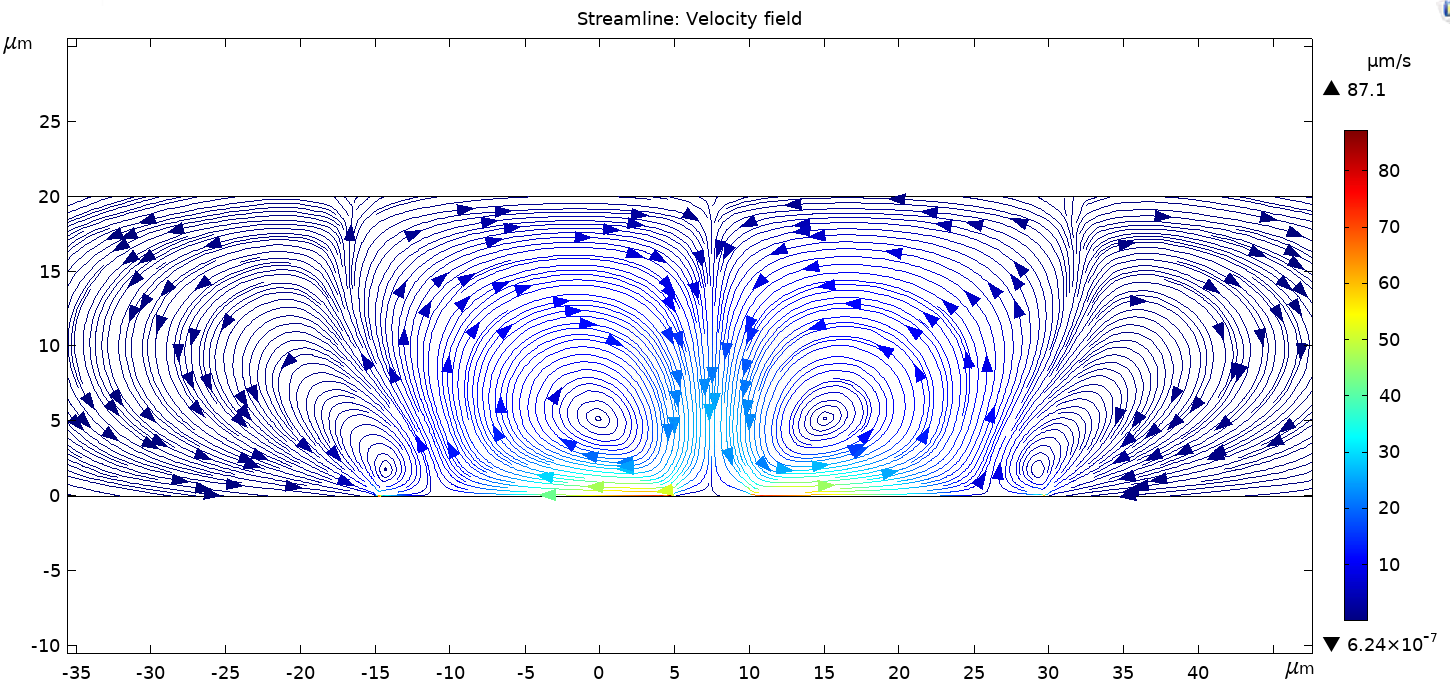
\includegraphics[scale=0.6]{streamline_equal.PNG}
    \caption{Streamline of the fluid velocity field generated by one symmetric electrode pair for the case $L = S$, $\mathrm{V0=10\,V}$}
    \label{fig:streamline_equal}
\end{figure*}

\begin{figure*}[htbp]
    \centering
    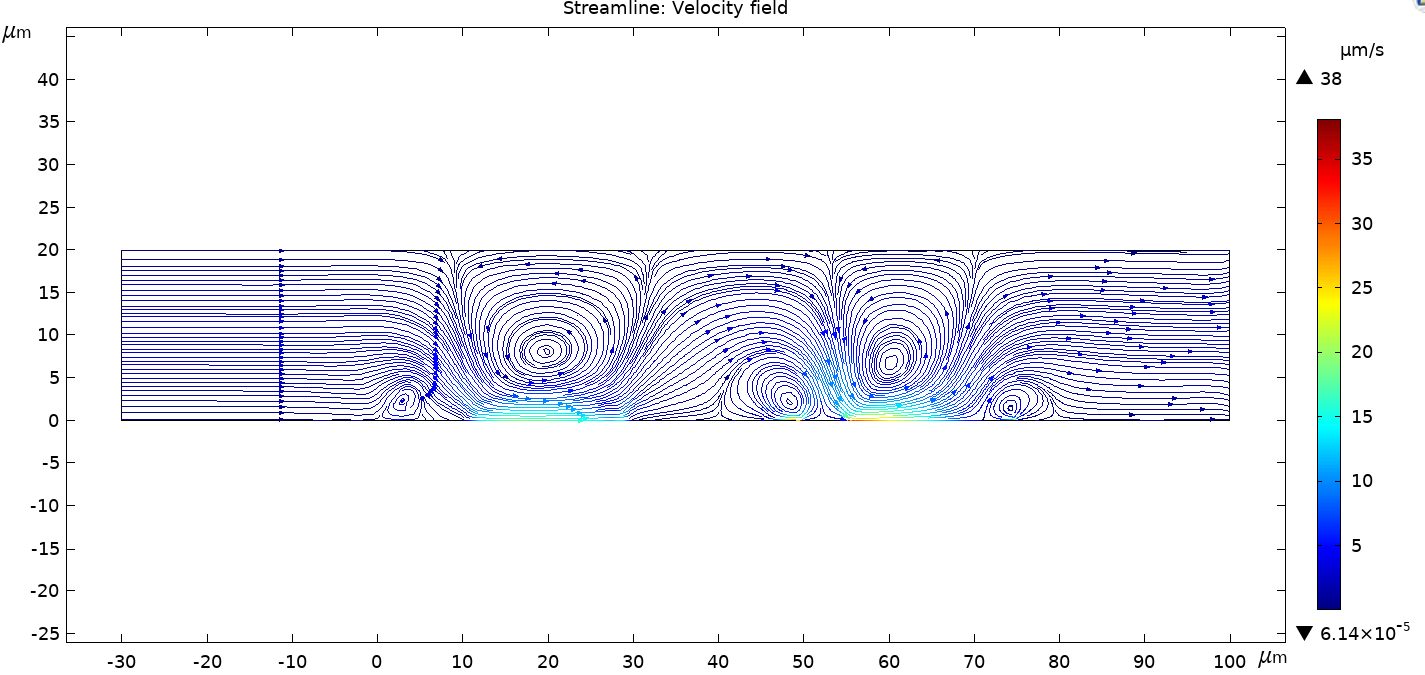
\includegraphics[scale=0.65]{streamline_two_pairs.PNG}
    \caption{Streamline of the fluid velocity field generated by two asymmetric electrode pairs for the case $L = 20\mu\,m, S = 5\mu m, G = 5\mu m, G_{1} = 15\mu m$, $\mathrm{V0=10\,V},c_{0} = 0.01 \textit{m}\,M$.}
    \label{fig:streamline_two}
\end{figure*}
Moreover, when the electrode pairs were added up to ten pairs, we got the maximum velocity shown as the legend in Fig.\ref{fig:streamline_ten} at the speed of 104 $\mu$m/s. However, the result is five times smaller than the experimental result\cite{Studer2004}.
\begin{figure*}[htbp]
    \centering
    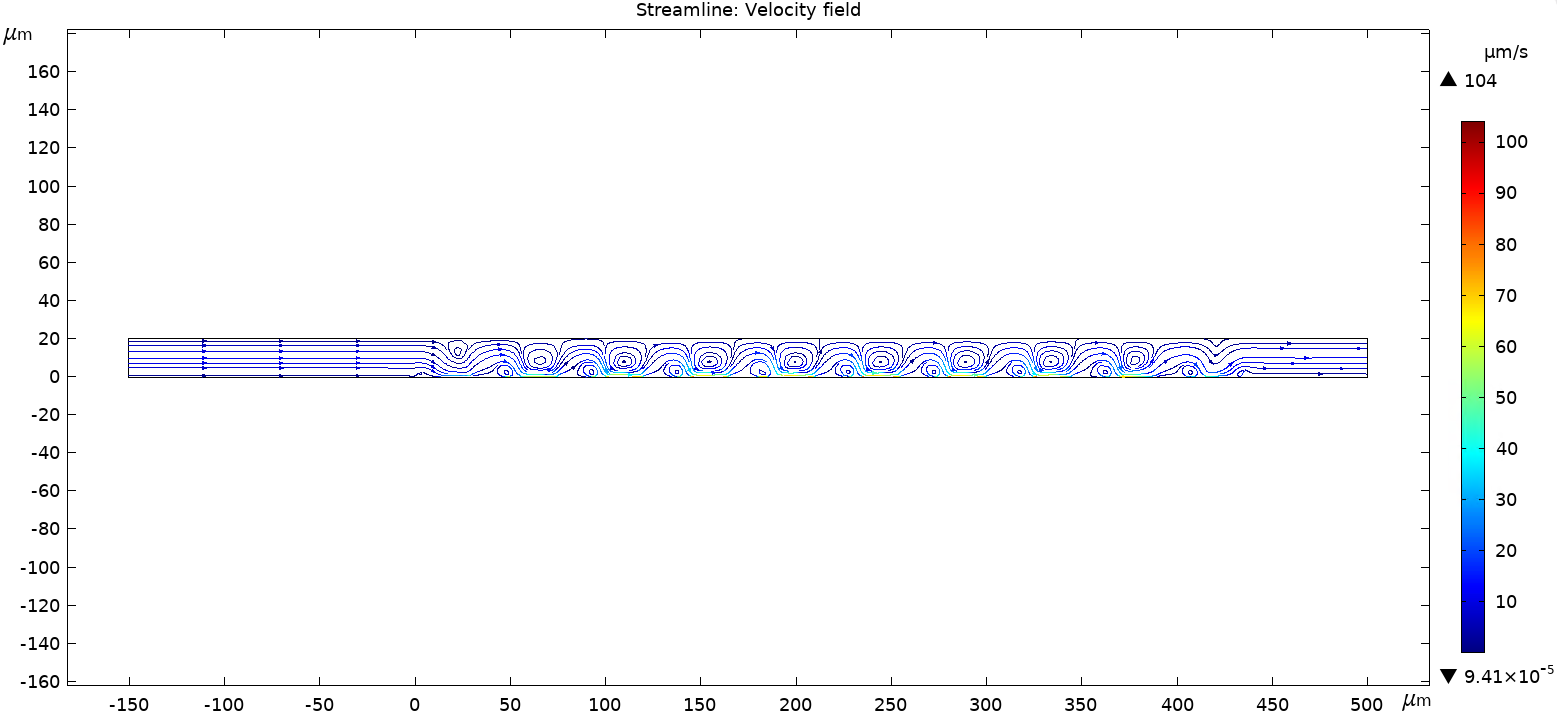
\includegraphics[scale=0.6]{streamline_ten_pairs.PNG}
    \caption{Streamline of the fluid velocity field generated by ten asymmetric electrode pairs for the case $L = 20\mu m, S = 5\mu m, G = 5\mu m, G_{1} = 15\mu m$, $\mathrm{V0=10\,V}, c_{0} = 0.01 \textit{m}M$}
    \label{fig:streamline_ten}
\end{figure*}
\begin{figure*}[htbp]
    \centering
    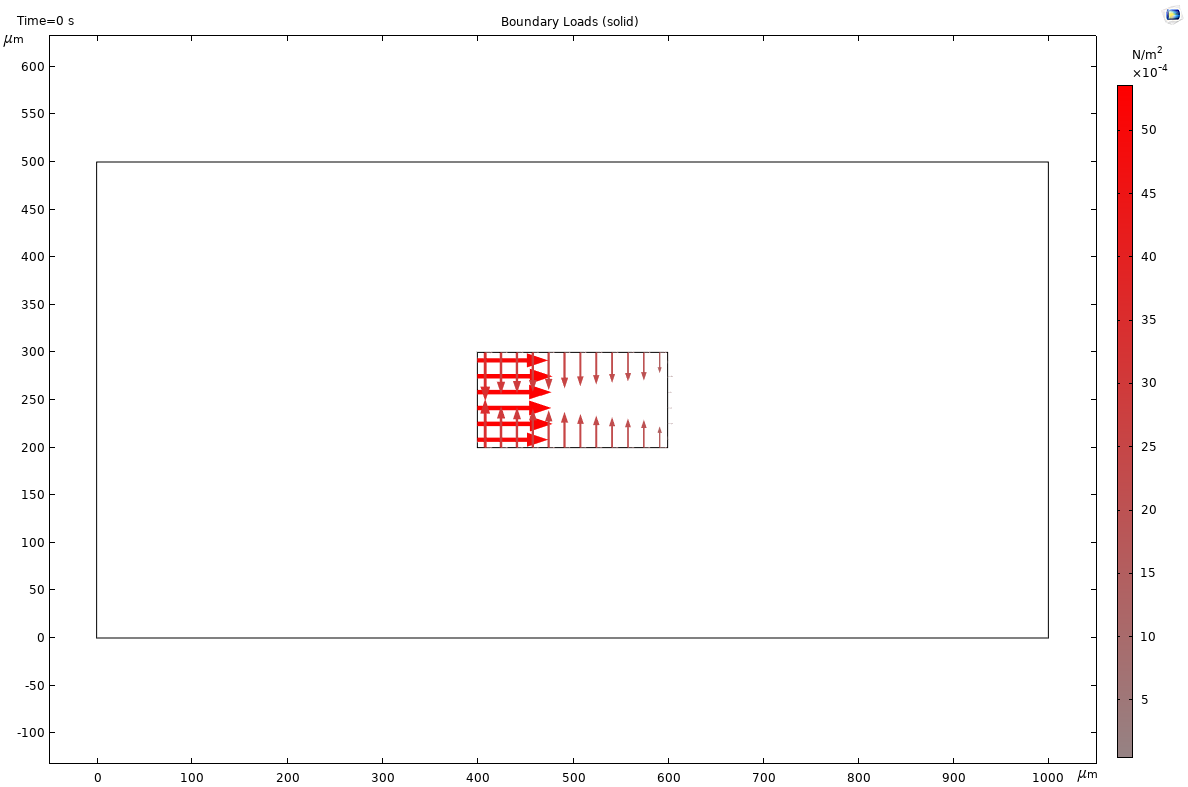
\includegraphics[scale=0.5]{loads.png}
    \caption{The boundary loads on the chip when the normal inflow velocity $U_0=5.6\,\mathrm{\mu m/s}$, the height of the tank $H=500\,\mathrm{\mu m}$, and the height of the chip $h=100\,\mathrm{\mu m}$.}
    \label{fig:loads}
\end{figure*}

Then, we moved on to predict the propulsion force and the forward speed of the devices when pumping. However, the considerable energy dissipation was difficult to predict quantitative. Hence, we considered the momentum provided by the electrodes instead. By Newton's second law, the impulse in the $x$ direction provided by the electrodes in a time interval $\Delta t$ is
\begin{equation}
    F\Delta t=(m_\text{f}+\Delta m_\text{f})(v_\text{f}+\Delta v_\text{f})-m_\text{f}v_\text{f},
\end{equation}
and by conservation of momentum in the $x$ direction,
\begin{equation}
    m_\text{f}v_\text{f}+m_\text{c}v_\text{c}=0,
\end{equation}
where $m_\text{f}$ is the mass of the fluid, $v_\text{f}$ is the average horizontal velocity of the fluid, $m_\text{c}$ is the mass of the chip, $v_\text{c}$ is the horizontal velocity of the chip. When $t=0.05\,\text{s}$, the increase in velocity $\Delta v_\text{f}=1.3323\times10^{-20}$, which can be neglected. Here, the height of the pipe $h=20\,\mathrm{\mu m}$, the width of the pipe $d=100\,\mathrm{\mu m}$, and the length of the pipe as $l=1030\,\mathrm{\mu m}$. Excluding the effect of dynamic viscosity, the total force applied on the fluid in the $x$ direction is provided by the electrodes. By simulation, when $t=0.05\,\text{s}$, $v_\text{f}=4.644\times10^{-6}\,\mathrm{m/s}$, then the force to the fluid per width unit $f$ is
\begin{equation}
    f=\frac{F}{d}=\rho_mhv_\text{f}=9.286\times10^{-8}\,\mathrm{N/m}.
\end{equation}

To estimate the resistance of the fluid to the device in open water area, a fluid-structure interaction (FSI) simulation was performed based on a larger scale. Due to the limitation of the simulation, instead of defining free surface at the top of the pipe as the interface between the air and the fluid, we placed the chip in the middle of the fluid and define sufficiently high pipe with a height of $500\,\mu\text{m}$ to ensure the velocity around it is approximately constant. By setting the outlet pressure as static $p_0=0\,\text{Pa}$ and substituting different value of normal inflow velocity $U_0$ at the inlet or doing the parameter sweep study, we found the the line integral of $x$ component of the normal applied boundary loads fsi1.F\_Anx or solid.F\_Ax on the front and the end side of the chip when $t=4.0000\,\text{s}$ denoted as $\mathbf{F}_\text{Lf}$ and $\mathbf{F}_\text{Le}$ together with their difference $\Delta\mathbf{F}_\text{L}$, which is shown in Table \ref{tab:v-loads}.
\begin{table}[H]
    \centering
    \begin{tabular}{|c|c|c|c|}
        \hline
        $U_0$ ($\mu$m/s)&$\mathbf{F}_\text{Lf}$ (N/m)&$\mathbf{F}_\text{Le}$ (N/m)&$\Delta\mathbf{F}_\text{L}$ (N/m)\\
        \hline
        1&$1.9525\times10^{-8}$&$2.9242\times10^{-9}$&$1.6601\times10^{-8}$\\
        \hline
        5&$9.7627\times10^{-8}$&$1.4620\times10^{-8}$&$8.3007\times10^{-8}$\\
        \hline
        5.5&$1.0739\times10^{-7}$&$1.6082\times10^{-8}$&$9.131\times10^{-8}$\\
        \hline
        5.6&$1.0934\times10^{-7}$&$1.6374\times10^{-8}$&$9.297\times10^{-8}$\\
        \hline
        6&$1.1715\times10^{-7}$&$1.7544\times10^{-8}$&$9.961\times10^{-8}$\\
        \hline
        10&$1.9526\times10^{-7}$&$2.9238\times10^{-8}$&$1.6602\times10^{-7}$\\
        \hline
    \end{tabular}
    \caption{The relationship between the normal inflow velocity $U_0$ and the integral of $x$ component of the normal applied boundary loads on the front and the end side of the chip.}
    \label{tab:v-loads}
    \vspace{-0.5cm}
\end{table}
From the table, we found that the velocity was approximately in direct proportion to the difference of the normal applied boundary loads on the front and the end side $\Delta\mathbf{F}_\text{L}$. Here, the object boundaries experience a load from the fluid, which is
\begin{equation}
    \mathbf{F}_\mathrm{T}=-\mathbf{n}\cdot(-p\mathbf{I}+\eta(\nabla\mathbf{u}+(\nabla\mathbf{u})^T)),
\end{equation}
where $\mathbf{n}$ is the normal vector to the boundary. This load represents a sum of pressure and viscous forces \cite{wang2007benchmarking}. Therefore, the velocity at which $\Delta\mathbf{F}_\text{L}$ is approximately equal to the force to the fluid per unit width $f$, i.e. the relative velocity of the chip to the fluid, is nearly $5.6\,\mathrm{\mu m/s}$.

When $U_0=5.6\,\mathrm{\mu m/s}$, the boundary loads on the chip are shown in Figure \ref{fig:loads}. From the graph, we find that for the same $y$ coordinate, the normal loads on the front and the end side of the chip are nearly the same, so our assumption is valid.
%===============================================================================
\section{Experiment}
\subsection{Materials and reagents}
NR-9 photoresist, propylene-glycol-monomethyl-ether-acetate (PGMEA) developer, Sylgard 184 PDMS (Polydimethylsiloxane) prepolymer base and curing agent were used. Acetone was purchased from Hushi (Shanghai, China). 2-Propanol ($\geq99.7\%$) was purchased from Shanghai Titan Scientific (Shanghai, China), 0.01 $m$M KCl Electrode protection solution, 10 mL 500 nm micro-sphere. 
\subsection{Electrode plate fabrication}
The fabrication of the electrode plate followed the procedure of common photolithography and lift-off. The masks (for the electrodes pairs and microfluidic channel) for photoetching are both of dimensions $3\times3\,\mathrm{inches}$ designed by KLayout (See Fig.\ref{f:klayout}). The glass substrate is of dimensions $25\times25\times0.5\,\mathrm{mm}$. The NR-9 photoresist layer spun on the glass substrate was around $100\,\mathrm{\mu m}$ determined by the spin coating at the speed of 4000 rpm for 40 s. After spinning, the substrate was soft-baked on the hot plate for 1 min at $140^{\circ}$C to dry the photoresist. When the substrate was cooled, it was exposed to the ultraviolet light for 14 s. Then, the post-bake of the substrate was performed at $110^{\circ}$C for 1 min. After the substrate was cooled, the photoresist was developed for 8s and then, it was immediately cleaned by the deionized water for 20s. When the electrode pairs observed by the microscope were straight and not short, this process was done.
\begin{figure}[H]
    \centering
    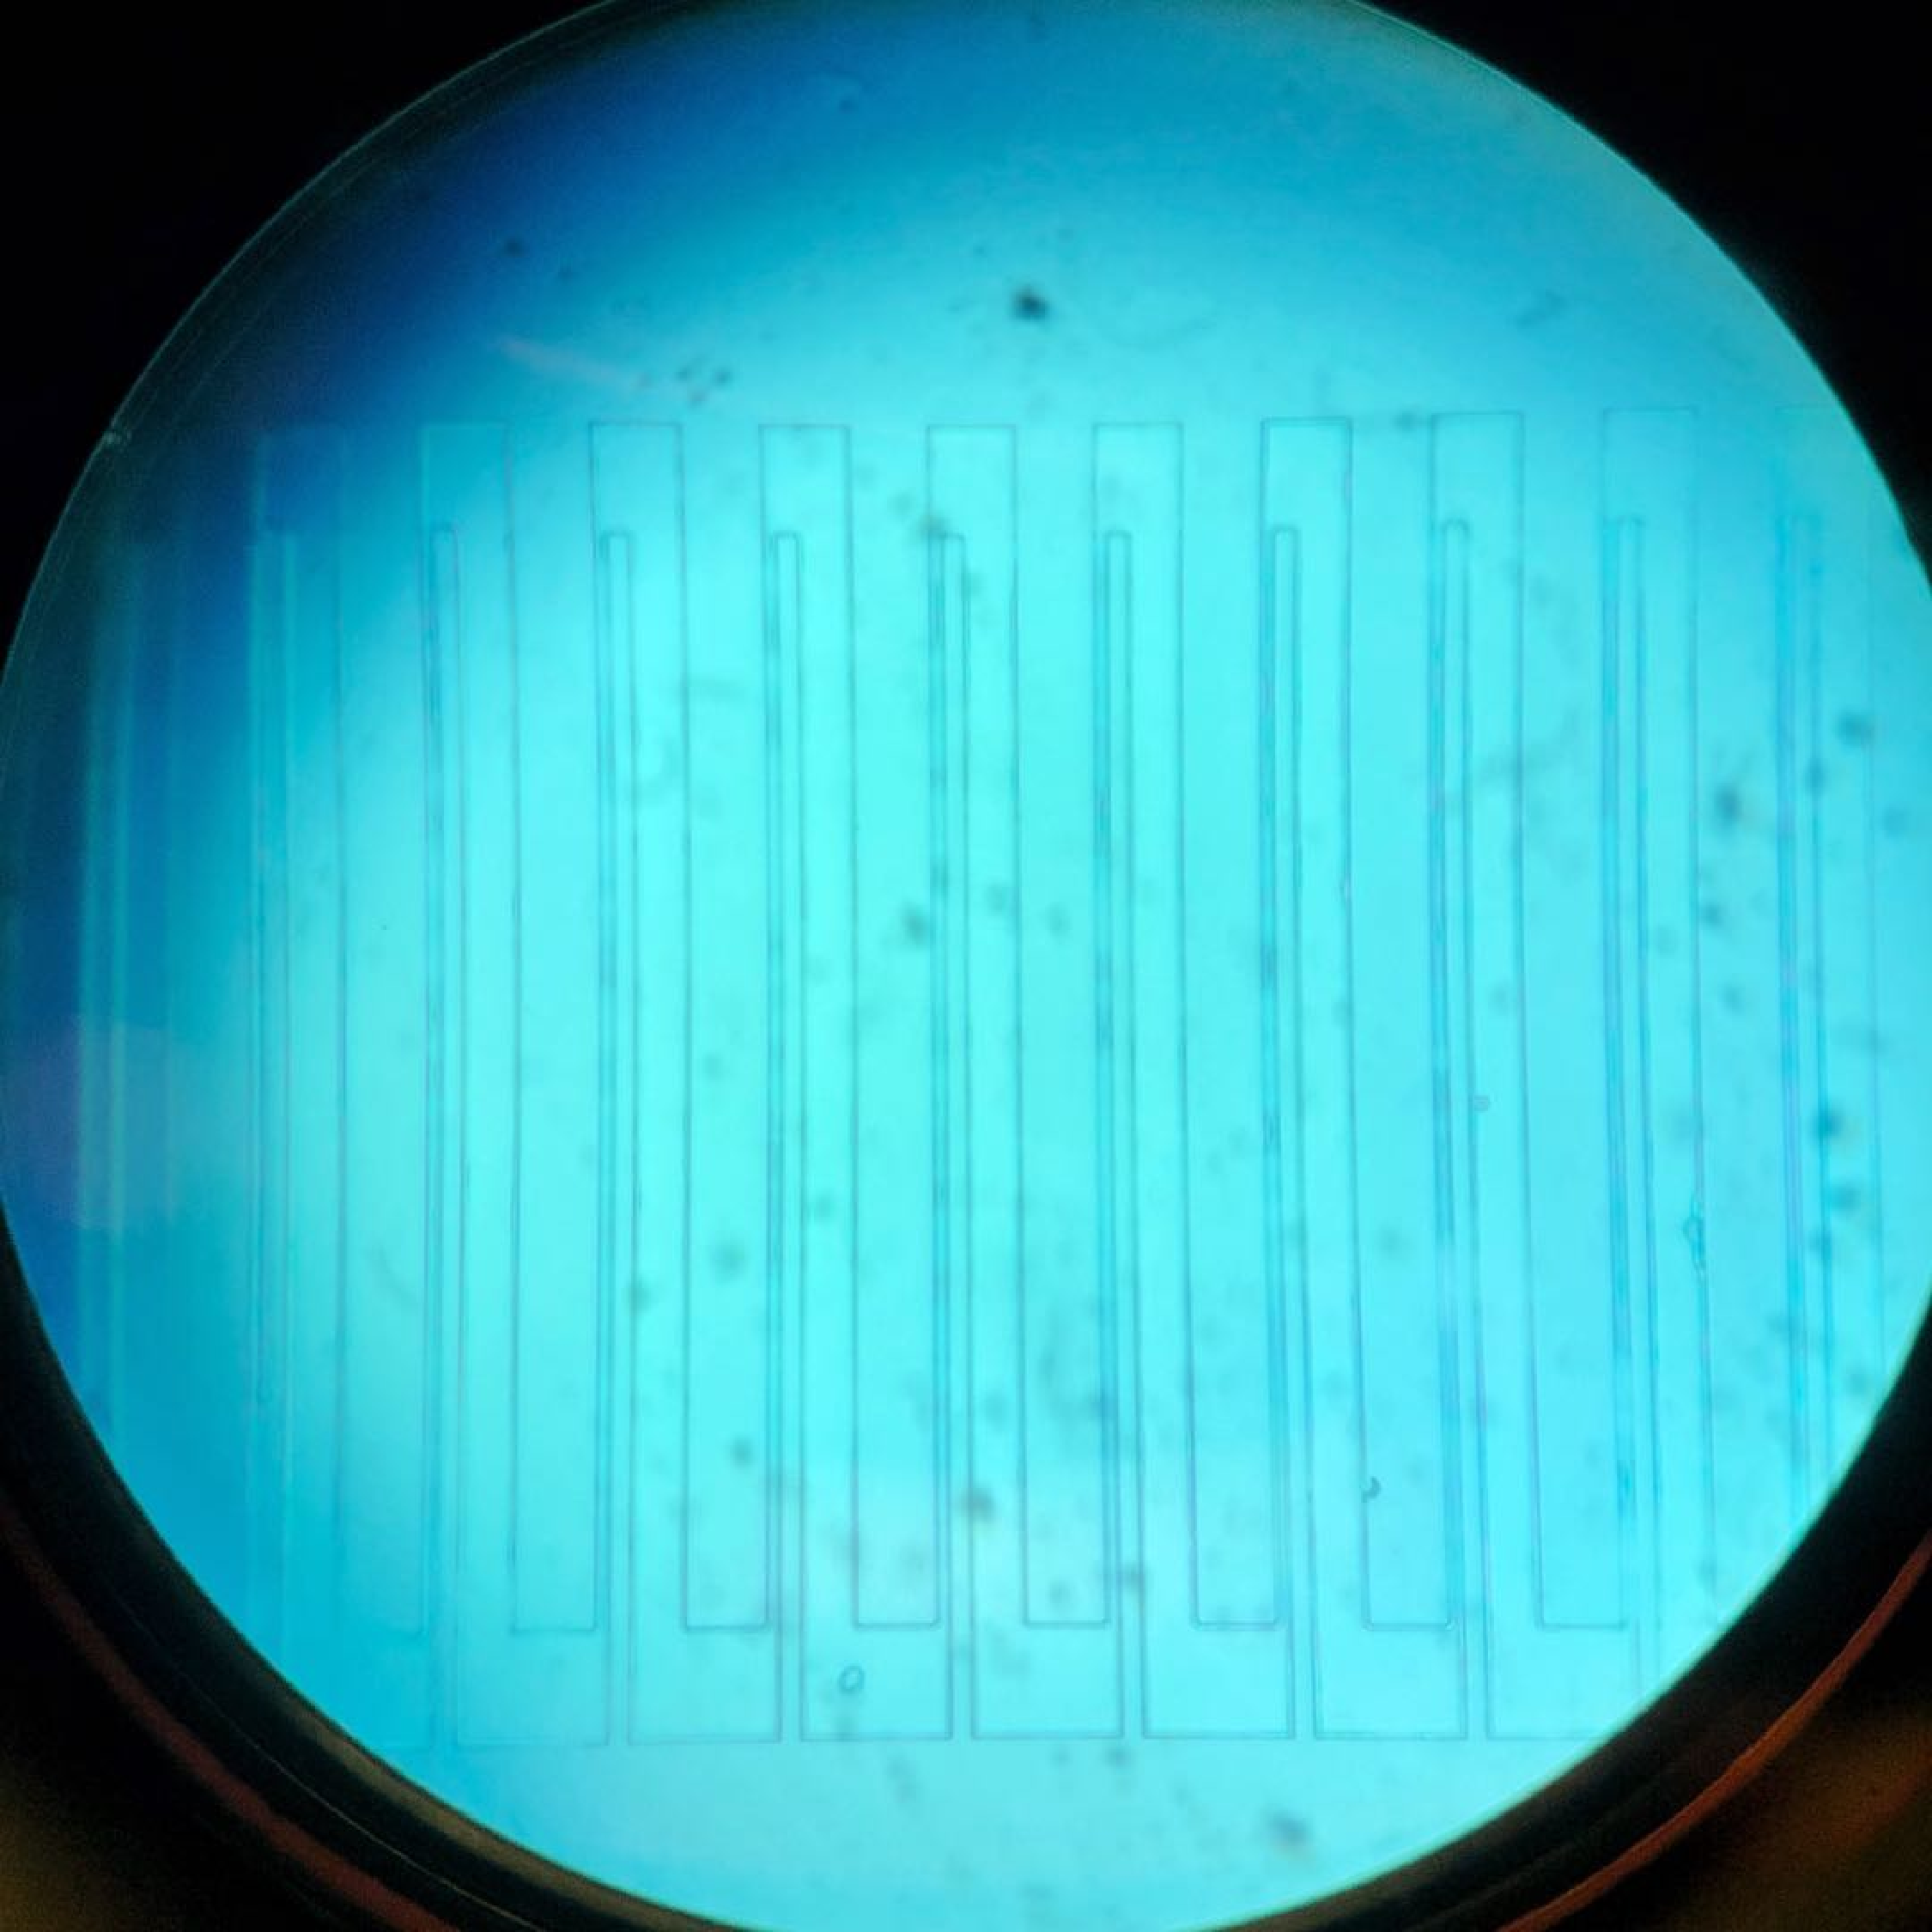
\includegraphics[width=0.4\textwidth]{good pattern.pdf}
	\caption{The electrode pairs on the glass substrate observed by the microscope.}
	\label{fig:electrode_pairs}
	\vspace{-0.8cm}
\end{figure}
Then we needed to make the glass substrate deposited with a layer of chromium with thickness of 5 nm followed by a layer of gold with thickness of 70 nm. The chromium layer can provide a stronger adhesion between the metal electrodes and the substrate. The photoresist pattern was transferred by life-off \cite{Studer2004}. The processed electrodes are shown in Fig.\ref{fig:electrode}.

\begin{figure*}[htbp]
    	\centering
    	\subfloat[A screen shot of fine electrodes pairs without short cut under the microscope.]{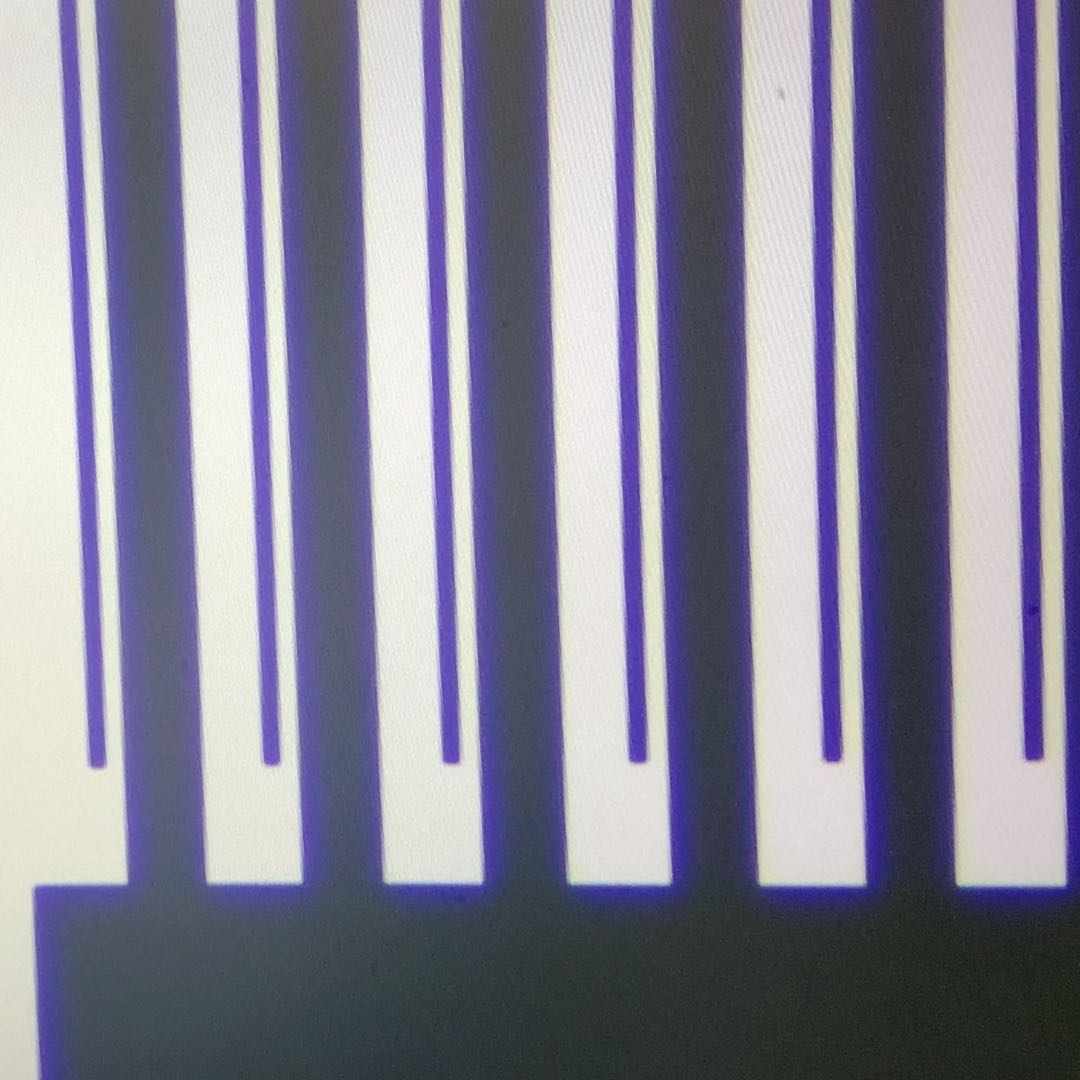
\includegraphics[width=0.36\textwidth]{fine_electrode.jpg}} \hspace{0.4in}%% \hspace{0.8in}  insert 0.4in space between two figures
    	\subfloat[A screen shot of a short cut electrodes pair without short cut under the  microscope.]{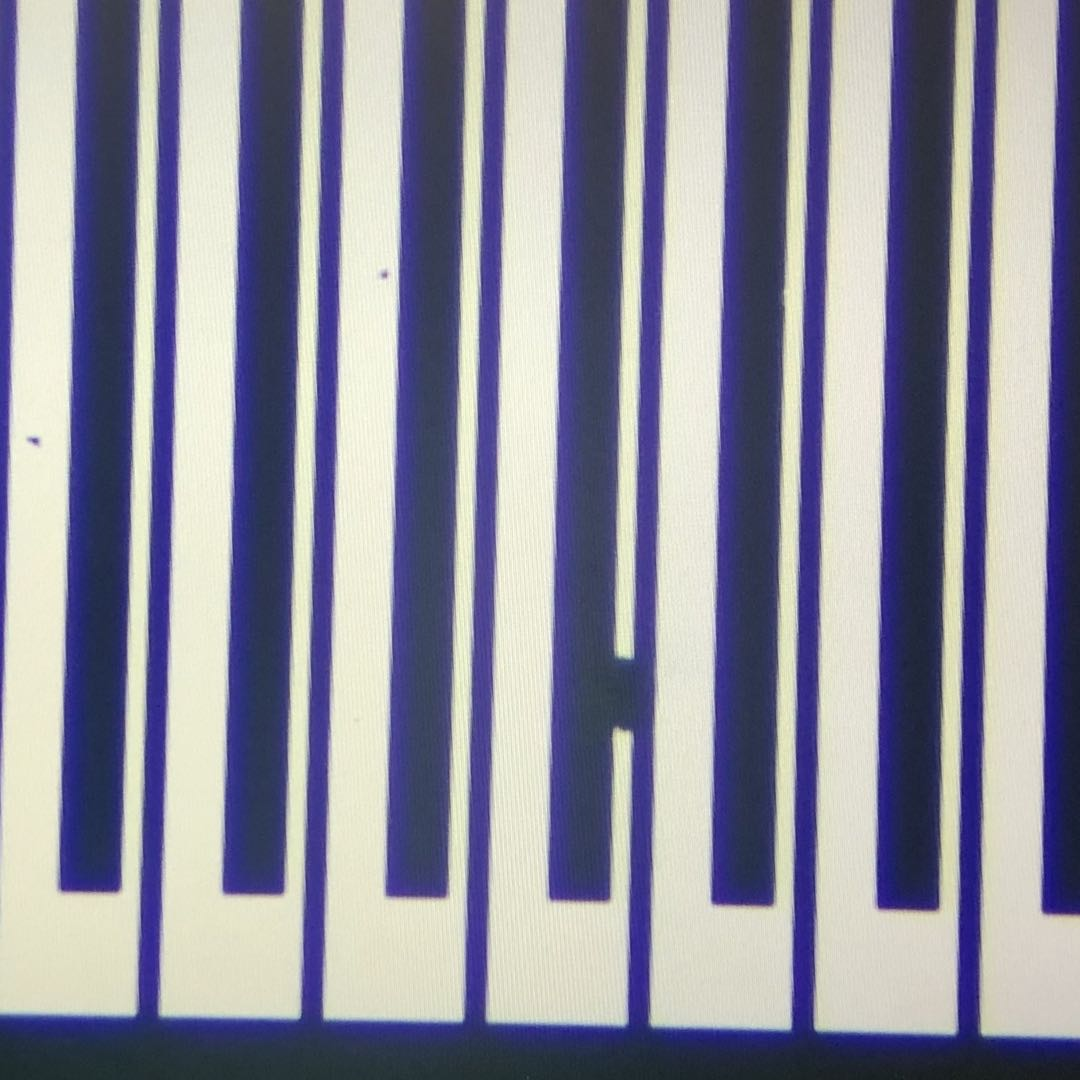
\includegraphics[width=0.36\textwidth]{short_cut.jpg}}
    	\caption{Screen shot of the asymmetric electrode pairs under the microscope.}
    	\label{fig:electrode}
\end{figure*} %% one column-figure;multi column- figure*
\subsection{Microfluidic channel fabrication and bonding}
\begin{figure}[htp]
    \centering
    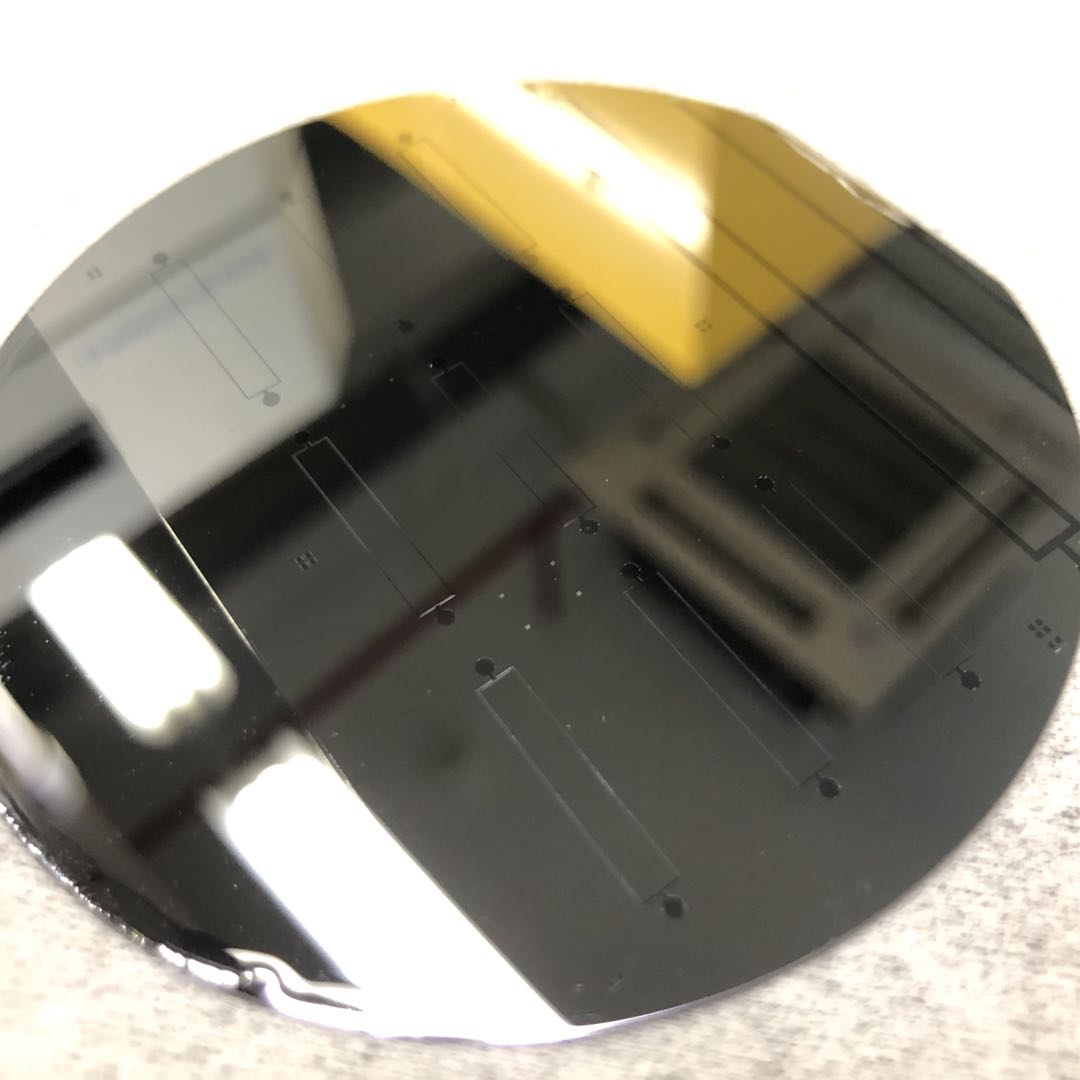
\includegraphics[scale = 0.18]{su8.jpg}
    \caption{Nine SU-8 moulds on a $3\times3\,\mathrm{inches}$ silicon wafer.}
    \label{fig:su8}
\end{figure}
We made nine SU-8 channel mould on a $3\times3\,\mathrm{inches}$ silicon wafer shown in Fig.\ref{fig:su8}.
We mixed $6 \mathrm{g}$ PDMS base and $0.6 \mathrm{g}$ curing agent by the ratio of 10:1 \cite{ou2009fabrication}. The mixing process could be accelerated by stirring or mechanical mixer at 2000 rpm for 1 min. The bubbles in the mixture were eliminated by the ultrasonic cleaner and vacuum drying oven for at least 30 minutes but not too long, since the PDMS might be more viscous. The PDMS prepolymer could be directly poured on the substrate, forming a 1.5 mm layer. It was better to pour it out near the substrate surface to avoid bubbles. Nevertheless, if there were bubbles, the substrate with PDMS should be degassed in the vacuum drying oven again. Baking could accelerate the solidification of the PDMS, so the substrate was baked on the hot plate at $85^{\circ}$C for 2 hours. However, to avoid bonding between the PDMS and the silicon substrate, we placed it for 24 hours exposed in the air to dry naturally. When the PDMS prepolymer was solidified significantly, it could be easily peeled off by tweezers or knives\cite{freeman2007manufacturing}. The microfluidic channel would be finished by punching small holes at the inlet and the outlet. Then, we needed to bond the substrate and the microfluidic channel. The substrate and the channel were cleaned by the oxygen plasma cleaner for 60 s with power of 29.6 W. Then the microfluidic channel was quickly placed on the substrate under microscope after alignment. There were 9 channels on the substrate in total if the PDMS fully covered the substrate. The channel used in experiment had the length of $1895\,\mathrm{\mu m}$, the width of $100\,\mathrm{\mu m}$, and the height of $20\,\mathrm{\mu m}$.
\subsection{Devices set up}
The substrate was pasted on a printed circuit board (PCB) of dimensions $36\times36\,\mathrm{mm}$. Using West Bond wire bonder, a set of the electrodes was connected to the pins of the PCB. A multimeter was connected to the two pins on the each part of the patterns to examine whether there were short circuits. We used a signal generator to apply a Sine signal for the devices. To clearly observe the microfluidic channel, a camera was placed on the eyepiece and the picture could be projected to a screen. The whole set up is shown in Fig.\ref{fig:set_up} and Fig.\ref{fig:pcb}.
\begin{figure*}[htbp]
    \centering
    \begin{overpic}
        [scale=0.21]{set_up.jpg}
        \put(10,46){\colorbox {white}{A.Viewing Screen}}
        \put(42,36){\colorbox {white}{B.Signal generator}}
        \put(45,7){\colorbox {white}{C.Microscope with the camera}}
        \put(75,26){\colorbox {white}{D.Viewing lamp}}
        \put(77,4){\colorbox {white}{E.Multimeter}}
    \end{overpic}
    \caption{The whole experimental set up.}
    \label{fig:set_up}
\end{figure*}

\begin{figure}[htbp]
    \centering
    \begin{overpic}
        [scale=0.26]{pcb.jpg}
        \put(6,55){\colorbox {white}{PCB board}}
        \put(15,75){\colorbox {white}{Object glass}}
        \put(44,39){\colorbox {white}{Microfluidic device}}
        \put(38,22){\colorbox {white}{Pin 1 wired to the positive pole}}
        \put(38,63){\colorbox {white}{Pin 2 wired to the negative pole}}
    \end{overpic}
    \caption{The microfluidic device on a PCB board.}
    \label{fig:pcb}
\end{figure}

\subsection{Fluid flow observation}
We filled the channel with 0.01 $\mathrm{m}M$ KCl solution mixed with 500 nm white micro-spheres by injection from the inlet of the channel. Then a Sine signal with the amplitude of 3 volts and frequency of 1.5 kHz generated by a signal generator was applied to the electrodes. From the viewing screen, we could observe the fluid flow in the microfluidic channel.

%===============================================================================
\section{Result}
To validate the developed mathematical result, we substituted three patterns used by Mpholo et al.\cite{Mpholo2003} to our simulation model to predict the maximum time average velocity and the optimal frequency of them.
\begin{figure}[htbp]
    \centering
    \setlength{\abovecaptionskip}{-0.3cm}
    % This file was created by matlab2tikz.
%
%The latest updates can be retrieved from
%  http://www.mathworks.com/matlabcentral/fileexchange/22022-matlab2tikz-matlab2tikz
%where you can also make suggestions and rate matlab2tikz.
%
\definecolor{mycolor1}{rgb}{0.00000,0.44700,0.74100}%
\definecolor{mycolor2}{rgb}{0.85000,0.32500,0.09800}%
\definecolor{mycolor3}{rgb}{0.92900,0.69400,0.12500}%
%
\begin{tikzpicture}[scale = 0.65]

\begin{axis}[%
thick,
width=4.521in,
height=3.559in,
at={(0.758in,0.488in)},
scale only axis,
clip=false,
xmode=log,
xmin=10,
xmax=100000,
xminorticks=true,
xlabel style={font=\color{white!15!black}},
xlabel={Frequency / Hz},
ymin=0,
ymax=70,
ylabel style={font=\color{white!15!black}},
ylabel={$\text{Simulated x-velocity / }\mu\text{m/s}$},
axis background/.style={fill=white},
title={Velocity vs. Frequency \& electrodes dimensions (1.0V)},
xmajorgrids,
xminorgrids,
ymajorgrids,
legend style={at={(0.03,0.97)}, anchor=north west, legend cell align=left, align=left, draw=white!15!black}
]
\addplot [color=mycolor1,very thick]
  table[row sep=crcr]{%
10	0.0163437627981899\\
10.9749876549306	0.0196802490565697\\
12.0450354025878	0.0236964171966023\\
13.2194114846603	0.0285300778561089\\
14.5082877849594	0.0343466924797213\\
15.9228279334109	0.0413447904514948\\
17.4752840000768	0.0497623886338541\\
19.1791026167249	0.0598845720248687\\
21.0490414451202	0.0720524067484627\\
23.1012970008316	0.0866733633191046\\
25.3536449397011	0.10423342461295\\
27.8255940220712	0.125311032715551\\
30.5385550883342	0.15059298252527\\
33.5160265093884	0.180892284802958\\
36.7837977182863	0.217167879928616\\
40.3701725859655	0.260545863373343\\
44.3062145758388	0.312341556706497\\
48.6260158006535	0.374081290985364\\
53.3669923120631	0.447522127945462\\
58.5702081805667	0.534666898592581\\
64.2807311728432	0.637770875707416\\
70.5480231071865	0.759335141013155\\
77.4263682681127	0.902080351918823\\
84.9753435908644	1.06889335764909\\
93.260334688322	1.26273831343387\\
102.353102189903	1.48652413231496\\
112.332403297803	1.74292201013095\\
123.284673944207	2.03413115063944\\
135.304777457981	2.36159833499236\\
148.496826225447	2.72570769193825\\
162.975083462064	3.12546992769898\\
178.864952905744	3.55825286045899\\
196.304065004027	4.0196033633847\\
215.443469003188	4.50321004641276\\
236.448941264541	5.00104255226357\\
259.502421139974	5.50367686068622\\
284.80358684358	6.00078105250433\\
312.571584968824	6.4817016928734\\
343.046928631492	6.93606810345687\\
376.493580679247	7.35432826027289\\
413.201240011533	7.72814737370135\\
453.487850812858	8.05063270119203\\
497.702356433211	8.31638562020764\\
546.227721768434	8.52141415003611\\
599.484250318941	8.66295922889985\\
657.933224657568	8.73929430154974\\
722.080901838546	8.74955222588698\\
792.482898353917	8.69361999539666\\
869.749002617783	8.57212395204899\\
954.548456661835	8.38650857312079\\
1047.61575278967	8.1391921206256\\
1149.75699539774	7.83376385722625\\
1261.85688306602	7.47517233964802\\
1384.88637139387	7.06984585582066\\
1519.91108295293	6.62568831987953\\
1668.10053720006	6.15190973973335\\
1830.73828029537	5.65867929623279\\
2009.23300256505	5.1566258928489\\
2205.13073990305	4.65624625593611\\
2420.12826479438	4.16730357942793\\
2656.08778294669	3.69830282551929\\
2915.05306282518	3.25611129570842\\
3199.26713779738	2.84576121498745\\
3511.19173421513	2.47043520181022\\
3853.52859371053	2.13160566459142\\
4229.2428743895	1.82928150382939\\
4641.58883361278	1.56231107893546\\
5094.13801481638	1.32869635702573\\
5590.81018251222	1.12588489308249\\
6135.90727341318	0.951019439485964\\
6734.15065775082	0.801136544526271\\
7390.72203352578	0.673314038236482\\
8111.30830789687	0.564772612567566\\
8902.15085445038	0.472939288390863\\
9770.09957299226	0.395481197827334\\
10722.6722201032	0.330317549963257\\
11768.11952435	0.275616487502923\\
12915.4966501488	0.229782189540768\\
14174.741629268	0.19143627481086\\
15556.7614393047	0.159396431922845\\
17073.5264747069	0.132654290120688\\
18738.1742286039	0.110353842098664\\
20565.1230834865	0.0917712130773859\\
22570.1971963392	0.0762962035528993\\
24770.7635599171	0.0634157830251751\\
27185.8824273294	0.0526995488496319\\
29836.4724028334	0.0437870638385645\\
32745.4916287773	0.0363769294716559\\
35938.1366380463	0.0302174243954214\\
39442.0605943766	0.0250985300049918\\
43287.6128108306	0.0208451690193466\\
47508.1016210279	0.0173114940527905\\
52140.0828799968	0.0143760778711165\\
57223.6765935022	0.0119378730980908\\
62802.9144183425	0.00991282522694888\\
68926.121043497	0.0082310380755357\\
75646.3327554629	0.00683440486196768\\
83021.7568131974	0.0056746306747897\\
91116.2756115491	0.00471158322653309\\
100000	0.00391191846404535\\
};
\addlegendentry{$\text{25-5-5}\mu\text{m}$}

\addplot [color=mycolor2,very thick]
  table[row sep=crcr]{%
10	0.00902554182805936\\
10.9749876549306	0.0108704174855486\\
12.0450354025878	0.0130921804178739\\
13.2194114846603	0.0157677268951875\\
14.5082877849594	0.0189895983916559\\
15.9228279334109	0.0228691449501796\\
17.4752840000768	0.0275403192441244\\
19.1791026167249	0.0331642230533205\\
21.0490414451202	0.0399345495269471\\
23.1012970008316	0.0480840892590338\\
25.3536449397011	0.0578924958419639\\
27.8255940220712	0.0696955369099639\\
30.5385550883342	0.0838960890264518\\
33.5160265093884	0.100977167724499\\
36.7837977182863	0.121517315186162\\
40.3701725859655	0.146208693562854\\
44.3062145758388	0.175878245766665\\
48.6260158006535	0.21151227863926\\
53.3669923120631	0.254284782477543\\
58.5702081805667	0.305589707066494\\
64.2807311728432	0.367077241378233\\
70.5480231071865	0.440693856465525\\
77.4263682681127	0.528725422470674\\
84.9753435908644	0.63384204314141\\
93.260334688322	0.759142296625487\\
102.353102189903	0.908193256793811\\
112.332403297803	1.0850609303541\\
123.284673944207	1.29432354973064\\
135.304777457981	1.54105755208993\\
148.496826225447	1.83078322875087\\
162.975083462064	2.16935434288018\\
178.864952905744	2.56277419483308\\
196.304065004027	3.01692075612981\\
215.443469003188	3.53716706349425\\
236.448941264541	4.12789172599127\\
259.502421139974	4.79188954234981\\
284.80358684358	5.52971416225793\\
312.571584968824	6.33901162075312\\
343.046928631492	7.21393050848206\\
376.493580679247	8.14471338292732\\
413.201240011533	9.11757494561559\\
453.487850812858	10.1149474780218\\
497.702356433211	11.1161215058802\\
546.227721768434	12.098238219988\\
599.484250318941	13.0375182097756\\
657.933224657568	13.9105611265905\\
722.080901838546	14.6955405042046\\
792.482898353917	15.373151488776\\
869.749002617783	15.9272356231182\\
954.548456661835	16.3450845819748\\
1047.61575278967	16.6174910007854\\
1149.75699539774	16.7386532060035\\
1261.85688306602	16.7060460439904\\
1384.88637139387	16.5203456139297\\
1519.91108295293	16.1854506231822\\
1668.10053720006	15.7085886492077\\
1830.73828029537	15.1004436765725\\
2009.23300256505	14.3752036407422\\
2205.13073990305	13.5504140542075\\
2420.12826479438	12.6465433058249\\
2656.08778294669	11.6862168832514\\
2915.05306282518	10.6931513834085\\
3199.26713779738	9.69089505100247\\
3511.19173421513	8.701536264966\\
3853.52859371053	7.74455681662335\\
4229.2428743895	6.83597825890762\\
4641.58883361278	5.98788768282772\\
5094.13801481638	5.20835482940426\\
5590.81018251222	4.50168726903122\\
6135.90727341318	3.86892908619164\\
6734.15065775082	3.30849513640327\\
7390.72203352578	2.81684263724275\\
8111.30830789687	2.38910528363813\\
8902.15085445038	2.01964281438803\\
9770.09957299226	1.70248415851529\\
10722.6722201032	1.43166142470859\\
11768.11952435	1.20144427328135\\
12915.4966501488	1.0064905157377\\
14174.741629268	0.841930706878447\\
15556.7614393047	0.703403646792698\\
17073.5264747069	0.587057414078423\\
18738.1742286039	0.489527731350371\\
20565.1230834865	0.407902684492593\\
22570.1971963392	0.339680370793545\\
24770.7635599171	0.282724049349317\\
27185.8824273294	0.235217814379906\\
29836.4724028334	0.195624658745131\\
32745.4916287773	0.162647970707386\\
35938.1366380463	0.135196939957346\\
39442.0605943766	0.112355974876879\\
43287.6128108306	0.0933579989213996\\
47508.1016210279	0.0775613582879441\\
52140.0828799968	0.0644300043443294\\
57223.6765935022	0.0535165897092793\\
62802.9144183425	0.0444481200821387\\
68926.121043497	0.0369138236052657\\
75646.3327554629	0.0306549280493683\\
83021.7568131974	0.0254560684165139\\
91116.2756115491	0.0211380804754506\\
100000	0.0175519673642521\\
};
\addlegendentry{$\text{15-3-3}\mu\text{m}$}

\addplot [color=mycolor3,very thick]
  table[row sep=crcr]{%
10	0.0052903175262844\\
10.9749876549306	0.00637201601155698\\
12.0450354025878	0.00767483994620804\\
13.2194114846603	0.00924397163523299\\
14.5082877849594	0.0111338159181116\\
15.9228279334109	0.0134098783694882\\
17.4752840000768	0.016151024069324\\
19.1791026167249	0.0194521931832877\\
21.0490414451202	0.0234276644731874\\
23.1012970008316	0.028214975460138\\
25.3536449397011	0.0339796287048269\\
27.8255940220712	0.0409207379866148\\
30.5385550883342	0.0492777964923533\\
33.5160265093884	0.0593387818626279\\
36.7837977182863	0.0714498503797063\\
40.3701725859655	0.0860269148062364\\
44.3062145758388	0.103569447129547\\
48.6260158006535	0.124676897883732\\
53.3669923120631	0.150068176046558\\
58.5702081805667	0.180604684584033\\
64.2807311728432	0.217317451316197\\
70.5480231071865	0.261438924668462\\
77.4263682681127	0.314440006531581\\
84.9753435908644	0.378072851380153\\
93.260334688322	0.454419845353138\\
102.353102189903	0.545948953764387\\
112.332403297803	0.65557523932326\\
123.284673944207	0.7867277383701\\
135.304777457981	0.943419952128494\\
148.496826225447	1.13032085954792\\
162.975083462064	1.35282147036063\\
178.864952905744	1.61708939669099\\
196.304065004027	1.93010064759935\\
215.443469003188	2.29963384993421\\
236.448941264541	2.73420755140806\\
259.502421139974	3.24293664409217\\
284.80358684358	3.83528017932003\\
312.571584968824	4.52065143641021\\
343.046928631492	5.30786421365268\\
376.493580679247	6.20439958241177\\
413.201240011533	7.21549739322351\\
453.487850812858	8.34310813644726\\
497.702356433211	9.58478210893607\\
546.227721768434	10.9326185342035\\
599.484250318941	12.3724362298037\\
657.933224657568	13.883344265816\\
722.080901838546	15.4378705436225\\
792.482898353917	17.0027402863959\\
869.749002617783	18.540291455989\\
954.548456661835	20.0103936990263\\
1047.61575278967	21.3726369226659\\
1149.75699539774	22.588508773448\\
1261.85688306602	23.6233041298964\\
1384.88637139387	24.4475958566328\\
1519.91108295293	25.0382140429227\\
1668.10053720006	25.3787913497744\\
1830.73828029537	25.4600020696087\\
2009.23300256505	25.2796360973512\\
2205.13073990305	24.8426092831555\\
2420.12826479438	24.1609365878503\\
2656.08778294669	23.2536105295562\\
2915.05306282518	22.1462629711087\\
3199.26713779738	20.8704673769832\\
3511.19173421513	19.4625743068521\\
3853.52859371053	17.9620611720712\\
4229.2428743895	16.4094950905471\\
4641.58883361278	14.8443180716241\\
5094.13801481638	13.3027288403116\\
5590.81018251222	11.8159321600785\\
6135.90727341318	10.4089560961627\\
6734.15065775082	9.10012518256114\\
7390.72203352578	7.90115915347872\\
8111.30830789687	6.81777487985288\\
8902.15085445038	5.85062062621013\\
9770.09957299226	4.99636693538981\\
10722.6722201032	4.24880562747366\\
11768.11952435	3.59985154545167\\
12915.4966501488	3.0403867360755\\
14174.741629268	2.56092468568023\\
15556.7614393047	2.15209922357369\\
17073.5264747069	1.80499877428348\\
18738.1742286039	1.51137386340948\\
20565.1230834865	1.26374688079229\\
22570.1971963392	1.05545058108953\\
24770.7635599171	0.880617568468362\\
27185.8824273294	0.734138340157869\\
29836.4724028334	0.611601086684714\\
32745.4916287773	0.509222712195727\\
35938.1366380463	0.423777548477269\\
39442.0605943766	0.352527956059967\\
43287.6128108306	0.293159336144538\\
47508.1016210279	0.243720899575917\\
52140.0828799968	0.202572739961097\\
57223.6765935022	0.168339239099036\\
62802.9144183425	0.13986851486085\\
68926.121043497	0.116197443335427\\
75646.3327554629	0.0965217028572979\\
83021.7568131974	0.0801702644732458\\
91116.2756115491	0.0665837682185172\\
100000	0.0552962612612395\\
};
\addlegendentry{$\text{5-2-2}\mu\text{m}$}

\node[right, align=left]
at (axis cs:15,42) {$\text{c}_\text{0}\text{ = 0.01mM}$};
\addplot [color=mycolor1, only marks, mark=o, mark options={very thick,solid, mycolor1}]
  table[row sep=crcr]{%
6000	15\\
};
\addlegendentry{25-5-5$\mu\text{m}$}

\addplot [color=mycolor2, only marks, mark=o, mark options={very thick,solid, mycolor2}]
  table[row sep=crcr]{%
14000	30\\
};
\addlegendentry{15-3-3$\mu\text{m}$}

\addplot [color=mycolor3, only marks, mark=o, mark options={very thick, solid, mycolor3}]
  table[row sep=crcr]{%
17000	60\\
};
\addlegendentry{5-2-2$\mu\text{m}$}

\end{axis}
\end{tikzpicture}%
    \caption{Plots of dependencies of the generated time average velocity on the frequencies, and the corresponding maximum average velocities got in the experiment.\cite{Mpholo2003}. The legend indicates the size of $large$ $electrode-gap-small$ $electrode$}
    \label{fig:compare_matlab}
    \vspace{-0.5cm}
\end{figure}
The simulation results, as shown in Fig.\ref{fig:compare_matlab}, indicate that as the ratio of the large electrode size and the small electrode size decreases, the optimal frequencies trend to shift toward larger value. What stands out in the plot is that the experimental results shown as the hollow dots on the plot give the same tendency, although the simulation results are nearly half times smaller than the experimental one.
If we now turn to the dependencies of the generated velocities on the applied voltage amplitude, shown in Fig.\ref{fig:potential}, we found that only the data subjected to the potential smaller than 4 volts that meets the experimental results in Stone's research\cite{Stone2004}. When the applied voltage amplitudes are beyond a boundary value, Stone observed a reversed fluid flow in the microfluidic channel, which is not shown in our prediction.

Then, to more intuitively observe the fluid flow in the channel with respect to the number of the electrode pairs, we demonstrated a multi-physics field in COMSOL Multiphysics mentioned in the Simulation section. As shown in Fig.\ref{fig:COMSOL_simu}, the more electrode pairs, the larger maximum velocity on the electrode surface. Nevertheless, when the number of the electrode pairs and the channel length continuously increases up to a hundred pairs, the model was unable to calculate the correct streamline. Compared with the experimental results\cite{Stone2004}\cite{Ribetto2012}, where the number of the electrode pairs reaches to a hundred, the simulation result is several times smaller than them.
\begin{figure}[htp]
    \centering
    \setlength{\abovecaptionskip}{-0.2cm}
    % This file was created by matlab2tikz.
%
%The latest updates can be retrieved from
%  http://www.mathworks.com/matlabcentral/fileexchange/22022-matlab2tikz-matlab2tikz
%where you can also make suggestions and rate matlab2tikz.
%
\definecolor{mycolor1}{rgb}{0.00000,0.44700,0.74100}%
%
\begin{tikzpicture}[scale=0.65]

\begin{axis}[%
thick,
width=4.521in,
height=3.566in,
at={(0.758in,0.481in)},
scale only axis,
xmin=1,
xmax=10,
xlabel style={font=\color{white!15!black}},
xlabel={Number of electrode pairs},
ymin=0,
ymax=120,
ylabel style={font=\color{white!15!black}},
ylabel={$\text{Simulated x-velocity / }\mu\text{m/s}$},
axis background/.style={fill=white},
title={Maximum velocity on the electrodes vs.Electrode pairs (1.0V)},
xmajorgrids,
ymajorgrids
]
\addplot [color={red}, only marks, mark size=3.3pt, mark=*, mark options={solid, red}, forget plot]
  table[row sep=crcr]{%
1	14.9\\
2	27.3\\
3	37.9\\
4	63.1\\
5	84.2\\
6	102\\
7	111\\
8	117\\
9	113\\
10	110\\
};
\node[right, align=left]
at (axis cs:1.3,115) {$\text{c}_\text{0}\text{ = 0.01mM}$};
\end{axis}

\begin{axis}[%
width=5.833in,
height=4.375in,
at={(0in,0in)},
scale only axis,
xmin=0,
xmax=1,
ymin=0,
ymax=1,
axis line style={draw=none},
ticks=none,
axis x line*=bottom,
axis y line*=left
]
\end{axis}
\end{tikzpicture}%
    \caption{Simulated maximum velocity on the electrode surface with respect to the number of electrode pairs by COMSOL Multiphysics at 1.0 $\mathrm{V}$ in 0.01 $m$M KCl solution.}
    \label{fig:COMSOL_simu}
    \vspace{-0.2cm}
\end{figure}
Finally, we experimentally observed the fluid flow inside the microfluidic channel shown as Fig.\ref{fig:flow}. Although the channel was not fully filled with the solution, we could recognize the flow by the large amount of bubbles due to fluid flow when the signal was applied to the device. The direction of the flow was from the small electrode toward the large electrode, which is satisfied with others' prediction \cite{ramos2003}.

Overall, these results suggest that our mathematical model implemented by MATLAB and COMSOL Multiphysics qualitatively predicted the dependencies of the generated velocities on the applied amplitudes and frequencies and the fluid flow above the electrodes. The prediction was later verified by the experimental observations.

\begin{figure}[H]
    	\centering
    	\subfloat[The fluid in the channel is still when there was no input signal.]{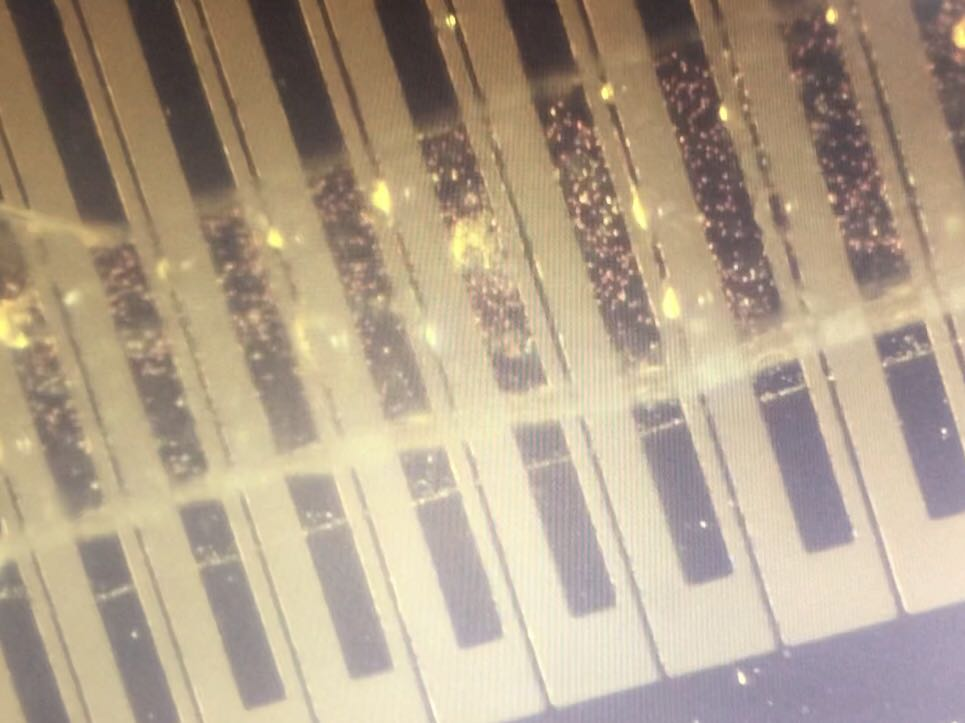
\includegraphics[width=0.4\textwidth]{fluid.jpg}} %% \hspace{0.8in}  insert 0.4in space between two figures
    	\\
    	\subfloat[The fluid flowed quickly with an applied Sine signal with the amplitude of 3 volts and frequency of 1.5 kHz.]{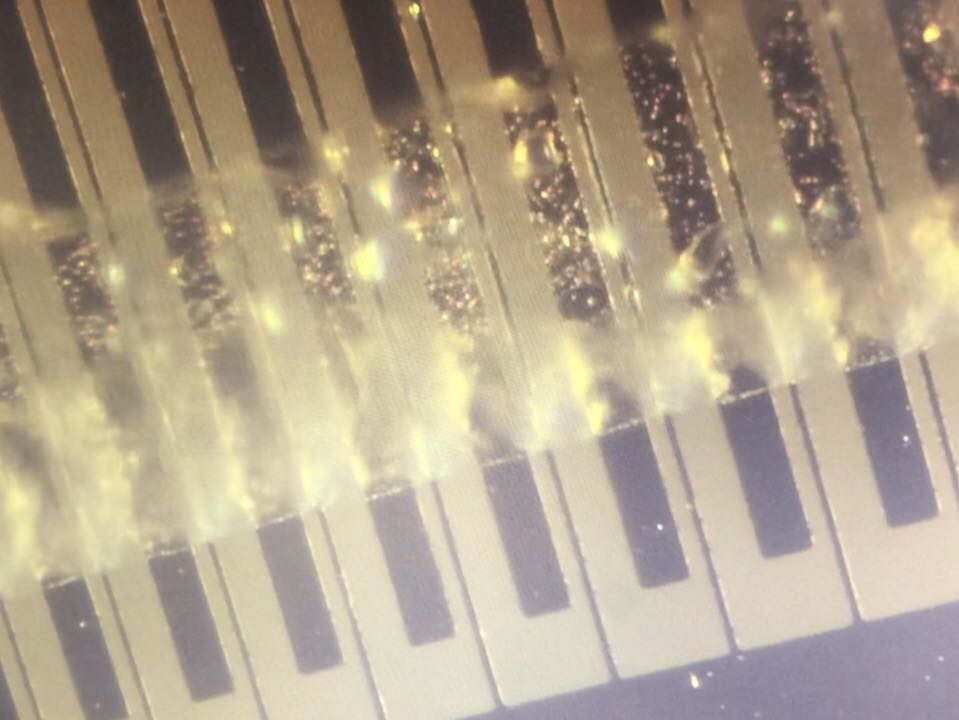
\includegraphics[width=0.4\textwidth]{fluid_flow.jpg}}
    	\\
    	\subfloat[The fluid flowed quickly with an applied Sine signal with the amplitude of 3.9 volts and frequency of 1.5 kHz. The small electrodes were burned under this working condition with very little liquid inside the channel.]{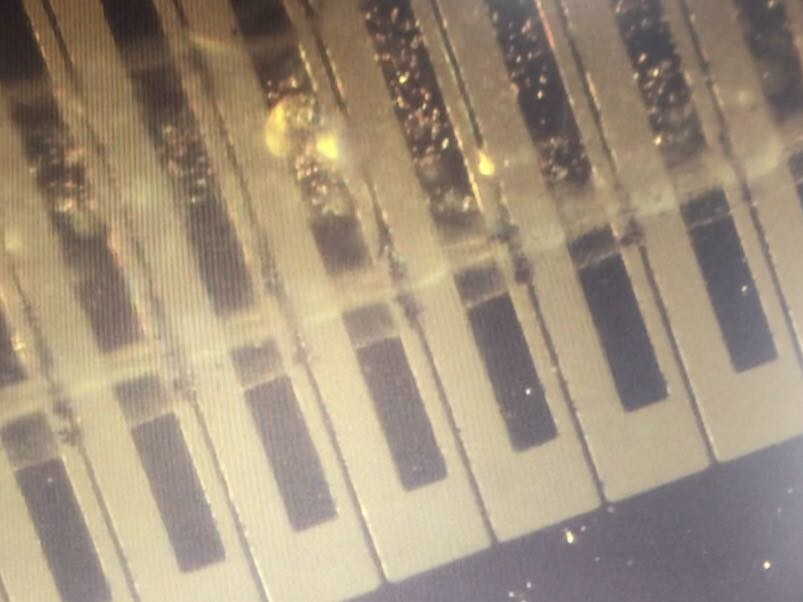
\includegraphics[width=0.4\textwidth]{burned_electrode.jpg}}
    	\caption{Screen shot of the asymmetric electrode pairs and the microfluidic channel half-filled with 0.01 $\mathrm{m}M$ KCl solution.}
    	\label{fig:flow}
\end{figure} %% one column-figure;multi column- figure*
\newpage
%===============================================================================
\section{Discussion}
\begin{figure*}[ht]
    \centering
    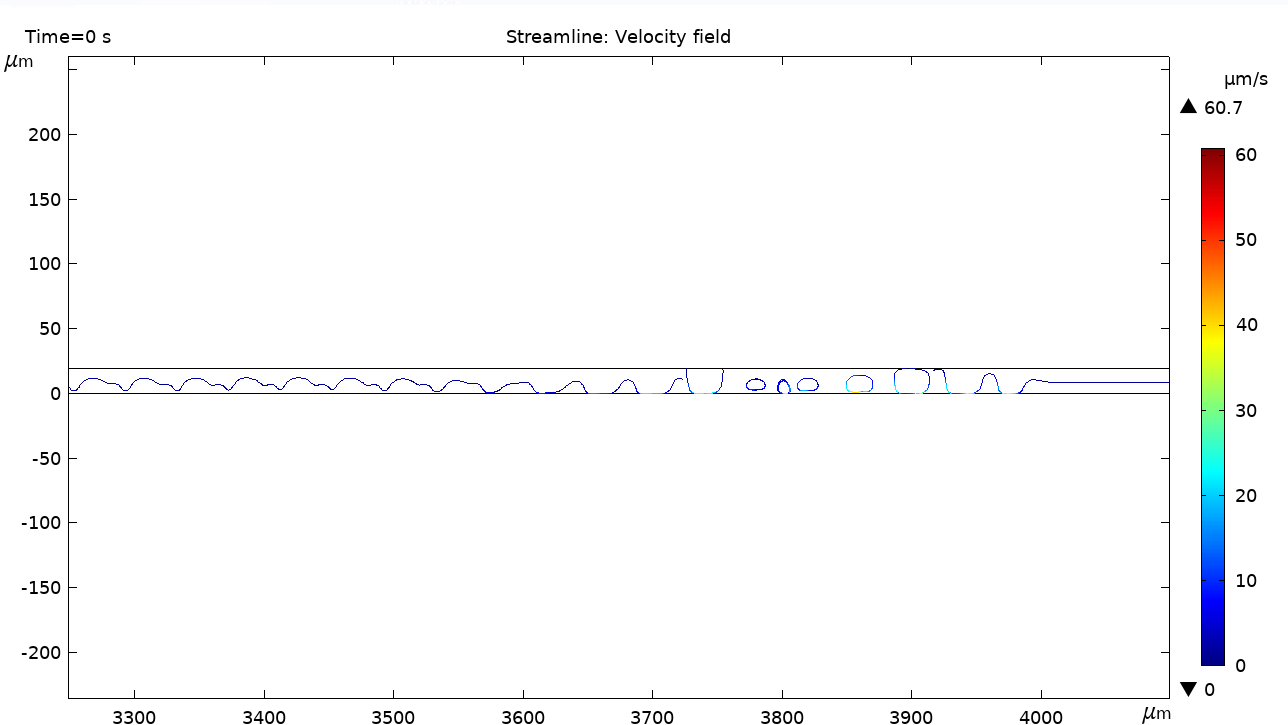
\includegraphics[scale=0.7]{100pairs.png}
    \caption{Streamline for the situation where a hundred electrode pairs are set up.}
    \label{fig:100pairs}
\end{figure*}
In our theoretical model, the geometric and kinematic equations were two-dimensional, neglecting the thickness of the electrodes. In reality, the double-layer approximation could be quite complex instead of being simply linear, for it cannot be estimated as a fixed capacitor when there is a larger applied voltage (\textgreater 1 V \cite{Brown2000}). It may be compressed significantly. However, for simplification, we took a certain Debye length to describe the double layer in the COMSOL simulation. Moreover, in our model, we assumed that the concentration of the solution in the microfluidic channel was unchanged without additional input ions from the electrodes due to electrolysis or other reactions. 

To be specific, the reduced analysis is easier, but the capacitance model is farther from its real electric properties. Besides, the real electric field lines are not semicircular, and we have to take their $y$ component into consideration. The precise model could be three-dimensional, directly derived from a set of basic fluid mechanics and electric equations with essential simplification:
\begin{equation}
    \left\{
        \begin{aligned}%{l} array environment dfrac two lines will overlap; left & is for aligned
            &\nabla^2\mathbf{\varphi}=-\dfrac{\rho_e}{\varepsilon},\\%\qquad\text{Poisson's equation for electrostatics}\\
            &\nabla\cdot\mathbf{J}=-\dfrac{\partial\rho_e}{\partial t},\\%\qquad\text{Continuity equation for current density}\\
            &\mathbf{J}=-\rho_n\mu\nabla\varphi-D\nabla\rho_e,\\
            %\qquad\text{Total current density for carrier diffusion}
            &\nabla\cdot\mathbf{u}=0,\\
            &-\nabla p+\rho_e\nabla\varphi+\mu\nabla^2\mathbf{u}=0,\\
            &\dfrac{\partial c}{\partial t}=\nabla\cdot(D\nabla c).
        \end{aligned}
    \right.
\end{equation}

The equations are Poisson's equation for electrostatics, continuity equation for current density, total current density for carrier diffusion, Navier-Stokes equations in non-inertial form for incompressible flow, and the convection-diffusion equation without sources or sinks of the variable of interest like chemical reactions and the coupled term $-\nabla\cdot(\mathbf{u}c)$, where $\rho_e=\rho_+-\rho_-$ and $\rho_n=\frac{\rho_++\rho_-}{2}$. Here, $\rho_+$ is the volume positive charge density and $\rho_-$ is the volume negative charge density. The boundary conditions are:
\begin{equation}
    \left\{
        \begin{aligned}
            &\varphi(y=0)=\frac{1}{2}V_0e^{i\omega t}\qquad\text{for }x\geq0,\\
            &\varphi(y=0)=-\frac{1}{2}V_0e^{i\omega t}\qquad\text{for }x<0,\\
            &\varphi(y\rightarrow\infty)\rightarrow0,\\
            &\rho_e(y\rightarrow\infty)\rightarrow0,\\
            &\rho_n(y\rightarrow\infty)\rightarrow\rho_{n0},\\
            &c(y\rightarrow\infty)\rightarrow0,\\
            &\dfrac{\partial c}{\partial y}\bigg|_{y=0}=0.
        \end{aligned}
    \right.
\end{equation}
Solving the simplified partial differential equations with more complex mathematical methods, a more precise result will be derived.

Due to several approximate treatment, the prediction generated velocities done by MATLAB are a few times smaller than the experiment result obtained in others' researches. And the fluid flow with larger applied voltage amplitude (see Fig.\ref{fig:potential}) poorly predict the reversed situation. 

Similarly, since the setting of the interfaces between the multi-physics fields was based on the mathematical model applied in MATLAB simulation, we found that when the applied voltage amplitude continuously increased, the corresponding velocity would rise to limitless value. Besides, for the Creeping flow field, we chose the $electroosmosis$ $velocity$ to describe the boundary condition between the electrode surface and the solution, but the given velocities were several times smaller than the real situations and this boundary condition would fail to predict the fluid flow when there were multiple electrode pairs (See Fig.\ref{fig:100pairs}). It means that we need to find a better finite element analysis method and the more precise boundary conditions.

On the other hand, to predict the velocity of the chip swimming in the open water area, we did not do direct simulation on it but tried to moreover do an equivalent simulation. In FSI simulation, the loads on the front and the end of the chip was not purely uniform. In reality, the chip will float on the water, so the loads on the upper part of the chip immersed in water would be less than the loads on the lower part, while the thrust in relation to the magnitude of velocity on the upper part would be much greater than that on the lower part. An improvement could be made by doing direct simulation using moving meshes and defining free surface between the water and the air.

For the experiment, we were in trouble when demoulding the PDMS from the SU-8 mould. At the first time, we made the SU-8 patterns on a glass wafer. After baking, the patterns were fully bonded to the PDMS. It should be noted that the SU-8 may have better adhesion to the silicon wafer than the glass wafer. Besides, it would be better if we divided the area first instead of tearing them at one time, since the adhesive force would pull the SU-8 up. The commonly-used solution is to do preliminary passivation treatment on the wafer using Chlorotrimethylsilane (TMCS) \cite{sun2016low}, but this reagent is highly toxic. We solved the problem of demoulding by ultrasonic cleaning of the wafer with the cleanser essence and deionized water 2-3 times before pouring the PDMS on it. Then let the PDMS dry at the room temperature for a day.

Also, we were in jam when we tried to bond the microfluidic channel to the substrate. Due to the limitation of the space under the microscope, it was hard to align the channel with the electrodes array on the substrate, which resulted in a weak bond. Unfortunately, in the experiment, due to the weak bonding, the channel was pulled apart from the substrate by the inflow. In Fig.\ref{fig:flow}, we observed that the fluid was spread all over the surface between the PDMS and the substrate. Therefore, we needed a better operation table so as to bond two parts more quickly to avoid the lose efficacy of the plasma surface. Then, we could continue the measurement of pumping performance in a tightly closed channel. Moreover, from the experiment result, the electro-osmosis flow under high voltages and frequencies was too fast to capture its dynamic. In order to measure the speed of the fluid flow, it would be better to use a high-speed camera to capture the micro-sphere in the fluid flow. Also, we expected to observe a plug flow profile in the channel to verify our theory.

At this stage, we are using wires and the huge signal generator to provide power to the microrobot. A preliminary point for further discussion is the integrated wireless power transfer (WPT) system. In our future plan, the device will be put in the open water area without wired outer power supply so that it can "swim" freely in the water. It will be integrated with a wireless power supply and corresponding control circuits. One solution is to integrate coils beside or under the electrodes shielded by a layer.

%===============================================================================
\section{Conclusion}
The KCl solution has been pumped at a high speed across two arrays of electrodes successfully by applying the ACEO theory.

A simple model has been presented and compared to the existed experimental results in other researches. This model was in qualitative agreement with the experimental observations. Also, we predicted the possibility of whether the pumping force generated by the ACEO pump can drive the microrobot forward, and expected that the microrobot might swim at a speed of 5.6 $\mu$m/s on the water. However, there are a number of approximations in the modeling process, which significantly effect the predictions of the model. In order to improve it, these approximations would need to be addressed. It would be necessary to include a non-linear description of the electrical double layer under a higher applied voltage, so as to better predict the compression of it, allowing its capacitance to vary with the instantaneous potential across it\cite{Brown2000}. Besides, the variation in the solution concentration would need to be modeled as well as the descriptions of the electric field lines, the current flow and the power consumption in the system. Finally, a better hydrodynamic model of the creeping flow in COMSOL simulation would have to be generated with more precise boundary conditions. It should be noted that, in the experiment, we observed the electrolysis of the electrodes, so that we would need to consider the charge injection at the electrodes in our model. 

In this research, we see a great potential of the ACEO pump, since it needs a relatively simple fabrication techniques, less post-processing, and requires only sever electrical connections to drive it. It can work under a low AC voltage which can be easily generated and work in a complex chemical environment. What's more, it was capable to integrated with other CMOS circuits. From the simulation model and other researches, there exists a set of optimal size of the electrodes to give a relatively high propulsion speed which is subjected to the applied voltages and frequencies. Hence this pumping technique is applicable to fluid control on semiconductor devices. The next stage of the research is to find the best settings and realize the wireless power transmission integration.

Eventually, our goal is to create IC chips or the silicon-based life-form that we can toss directly into the ocean or water areas and program their motion collectively to executes tasks assigned by users. 
%===============================================================================
\bibliographystyle{IEEEtran}
\bibliography{reference} 
\onecolumn
%===============================================================================
\appendices
\section{MATLAB scripts}
We simulated the dependencies of the generated velocity on the applied AC frequency, the voltage amplitude and the concentration of the electrolyte. The present scripts follow Ribetto's work\cite{Ribetto2012}, which computes the average velocity generated on the electrode surface according to the theory presented by Brown\textit{et~al.} \cite{Brown2000}.

%===============================================================================
\subsection{Velocities vs. Frequencies and Dimensions}
\lstinputlisting[
label=1:test1,
caption=v\_f\_dimension\_test1.m.
]{v_f_dimension_test1.m}

\lstinputlisting[
label=2:test2,
caption=v\_f\_dimension\_test2.m.
]{v_f_dimension_test2.m}

\subsection{Velocities vs. Frequencies and Concentration}
\lstinputlisting[
label=3:concentration,
caption=v\_f\_concentration.m
]{v_f_concentration.m}

\subsection{Velocities vs. Frequencies and Potential}
\lstinputlisting[
label=4:potential,
caption=v\_potential\_f.m
]{v_potential_f.m}

%===============================================================================
\section{Experimental Procedure}
%-------------------------------------------------------------------------------
\subsection{Electrodes Loop Design}
The asymmetric electrodes arrays loop for pumping is shown in Figure~\ref{f:klayout}.
\begin{figure}[htbp]
\begin{center}
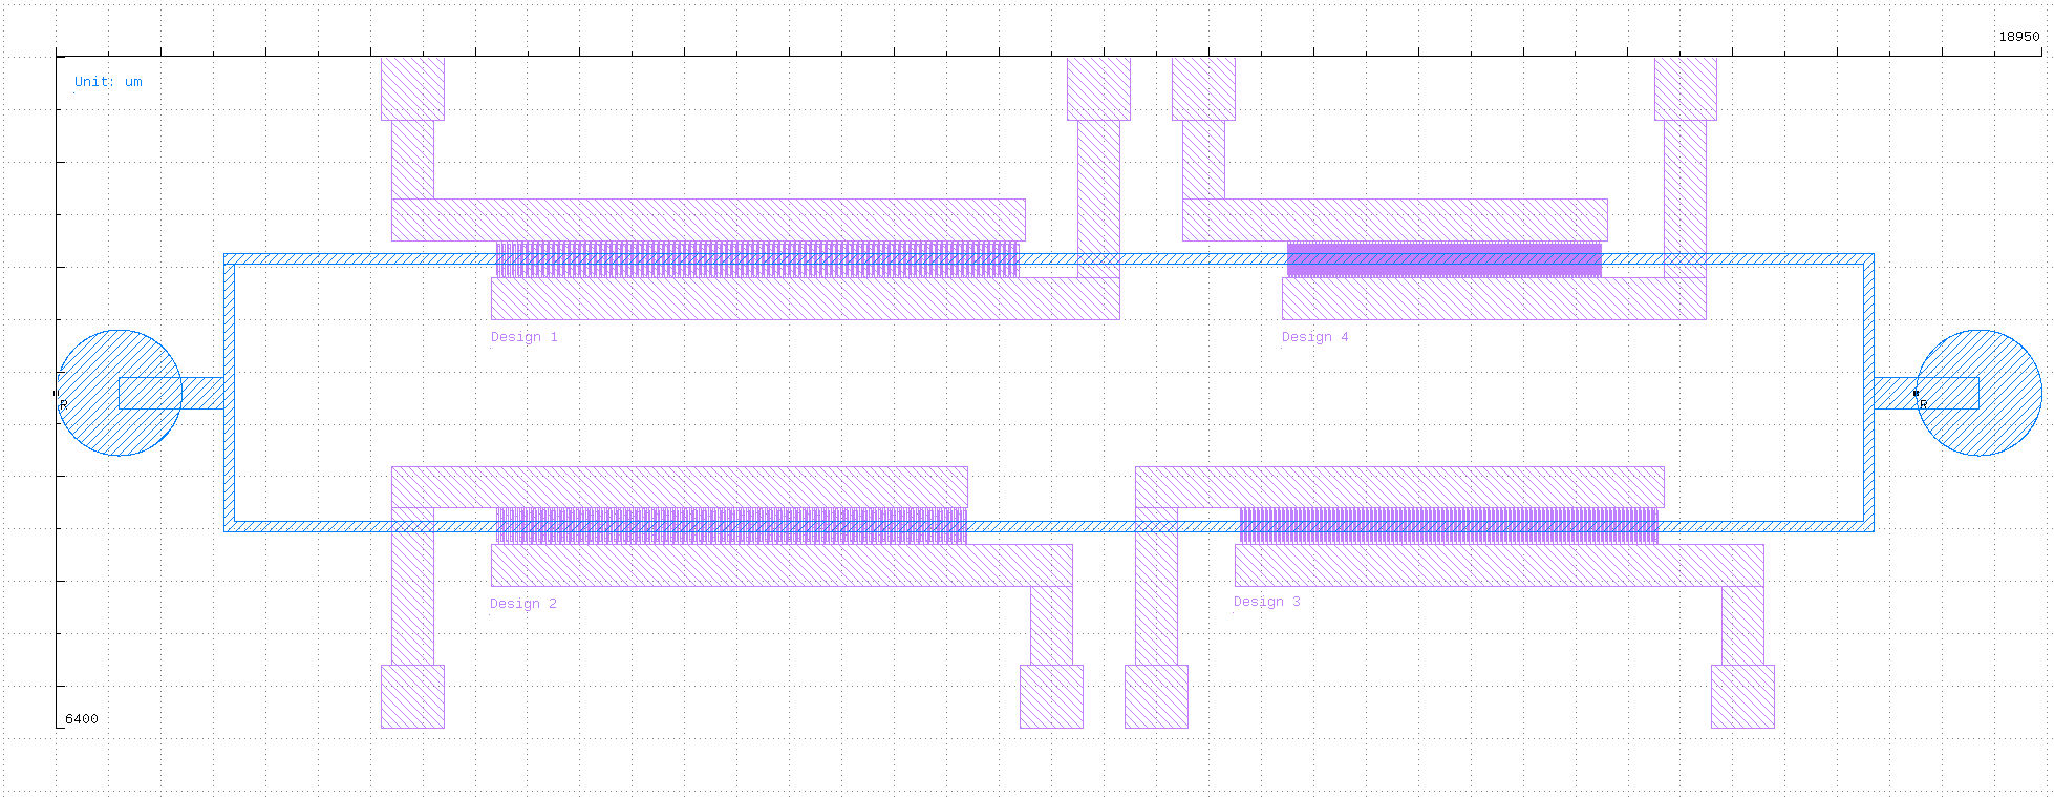
\includegraphics[width=0.7\textwidth]{klayout_design.pdf}
\caption{\label{f:klayout}A overview of the asymmetric electrodes arrays loop. The blue pattern represent the microfludic channel and the purple patterns represent the electrodes. The total length is 1.895 cm, and the total width is 0.64 cm.}
\end{center}
\end{figure}
\par The microfluidic channel is 20 \textmu m depth and 100 \textmu m width in our design. The loop is composed of four groups of the electrodes array each of which has 100 pairs of asymmetric electrodes, and a microfluidic channel. Each pair of asymmetric electrodes is subjected to an ac potential difference. The four patterns of electrode are shown in Table~\ref{t:pattern}.
\begin{table}[htbp]
\centering
\begin{tabular}{llllll} 
\toprule
\textbf{Pattern} & \textbf{\textit{L}(\textmu m)} & \textbf{\textit{S}(\textmu m)} & \textbf{\textit{G}(\textmu m)} & \textbf{\textit{G1}(\textmu m)} & \textbf{Number of Pairs}  \\ 
\hline
Design 1         & 25                  & 5                   & 5                   & 15                   & 100                       \\
Design 2         & 20                  & 5                   & 5                   & 15                   & 100                       \\
Design 3         & 15                  & 5                   & 5                   & 15                   & 100                       \\
Design 4         & 10                  & 6                   & 4                   & 10                   & 100                       \\ 
\hline
Electrode length \textbf{(\textmu m)} & 320                 &                     &                     &                      &                           \\
\bottomrule
\end{tabular}
\caption{\label{t:pattern}Four patterns of electrodes size used in the loop.}
\end{table}
\subsection{Electrodes fabrication}
Electrode arrays were fabricated on a high-temperature-resistance-glass substrate of dimensions 30 x 30 mm. The electrodes patterns were transferred from the mask to the substrate by standard photo-lithography. A 5 nm thick layer of chrome followed by a 40 nm thick layer of gold (Au) were deposited by deposition on the top of the photo-resist patterns. The photo-resist pattern was then transferred in metal by lift-off.
\begin{enumerate}
    \item Pretreatment of the substrate\\
    The four glass substrates were cleaned with acetone,  isopropanol alcohol (IPA), and deionized water for 10 minutes respectively in the ultrasonic cleaning machine. Then they were dried by the air gun.
    \begin{figure}[H]
    	\centering
    	\subfloat[The power panel.]{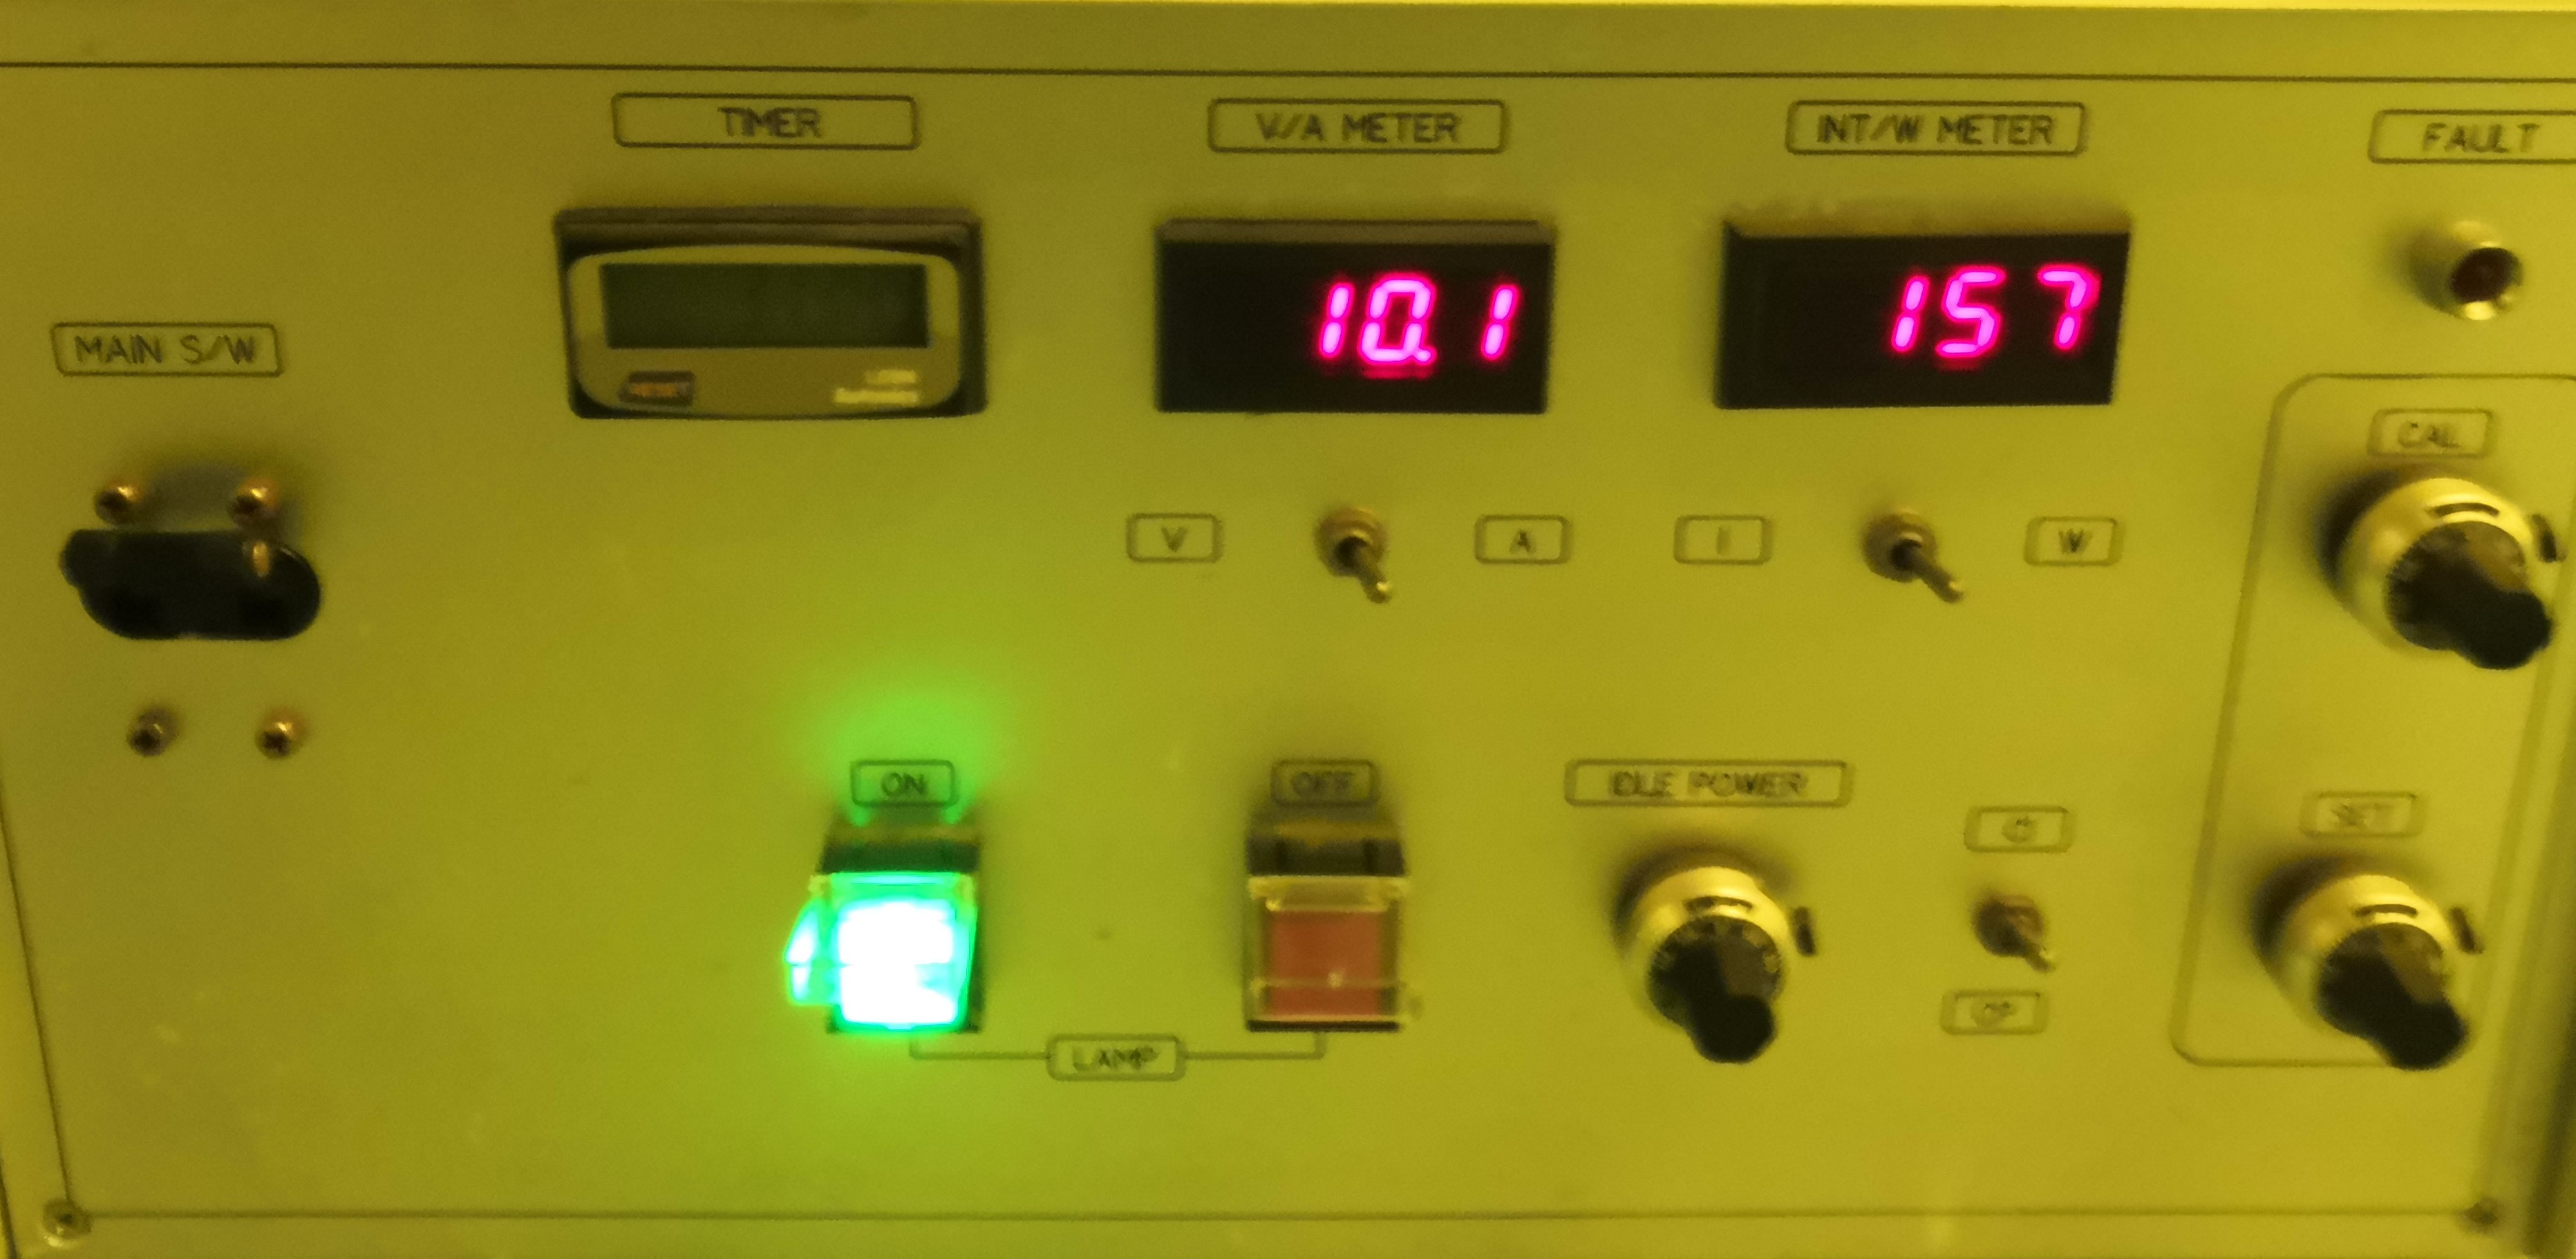
\includegraphics[width=0.3\textwidth]{EM_power_panel.jpg}}\hspace{0.4in}
    	\subfloat[The control panel.]{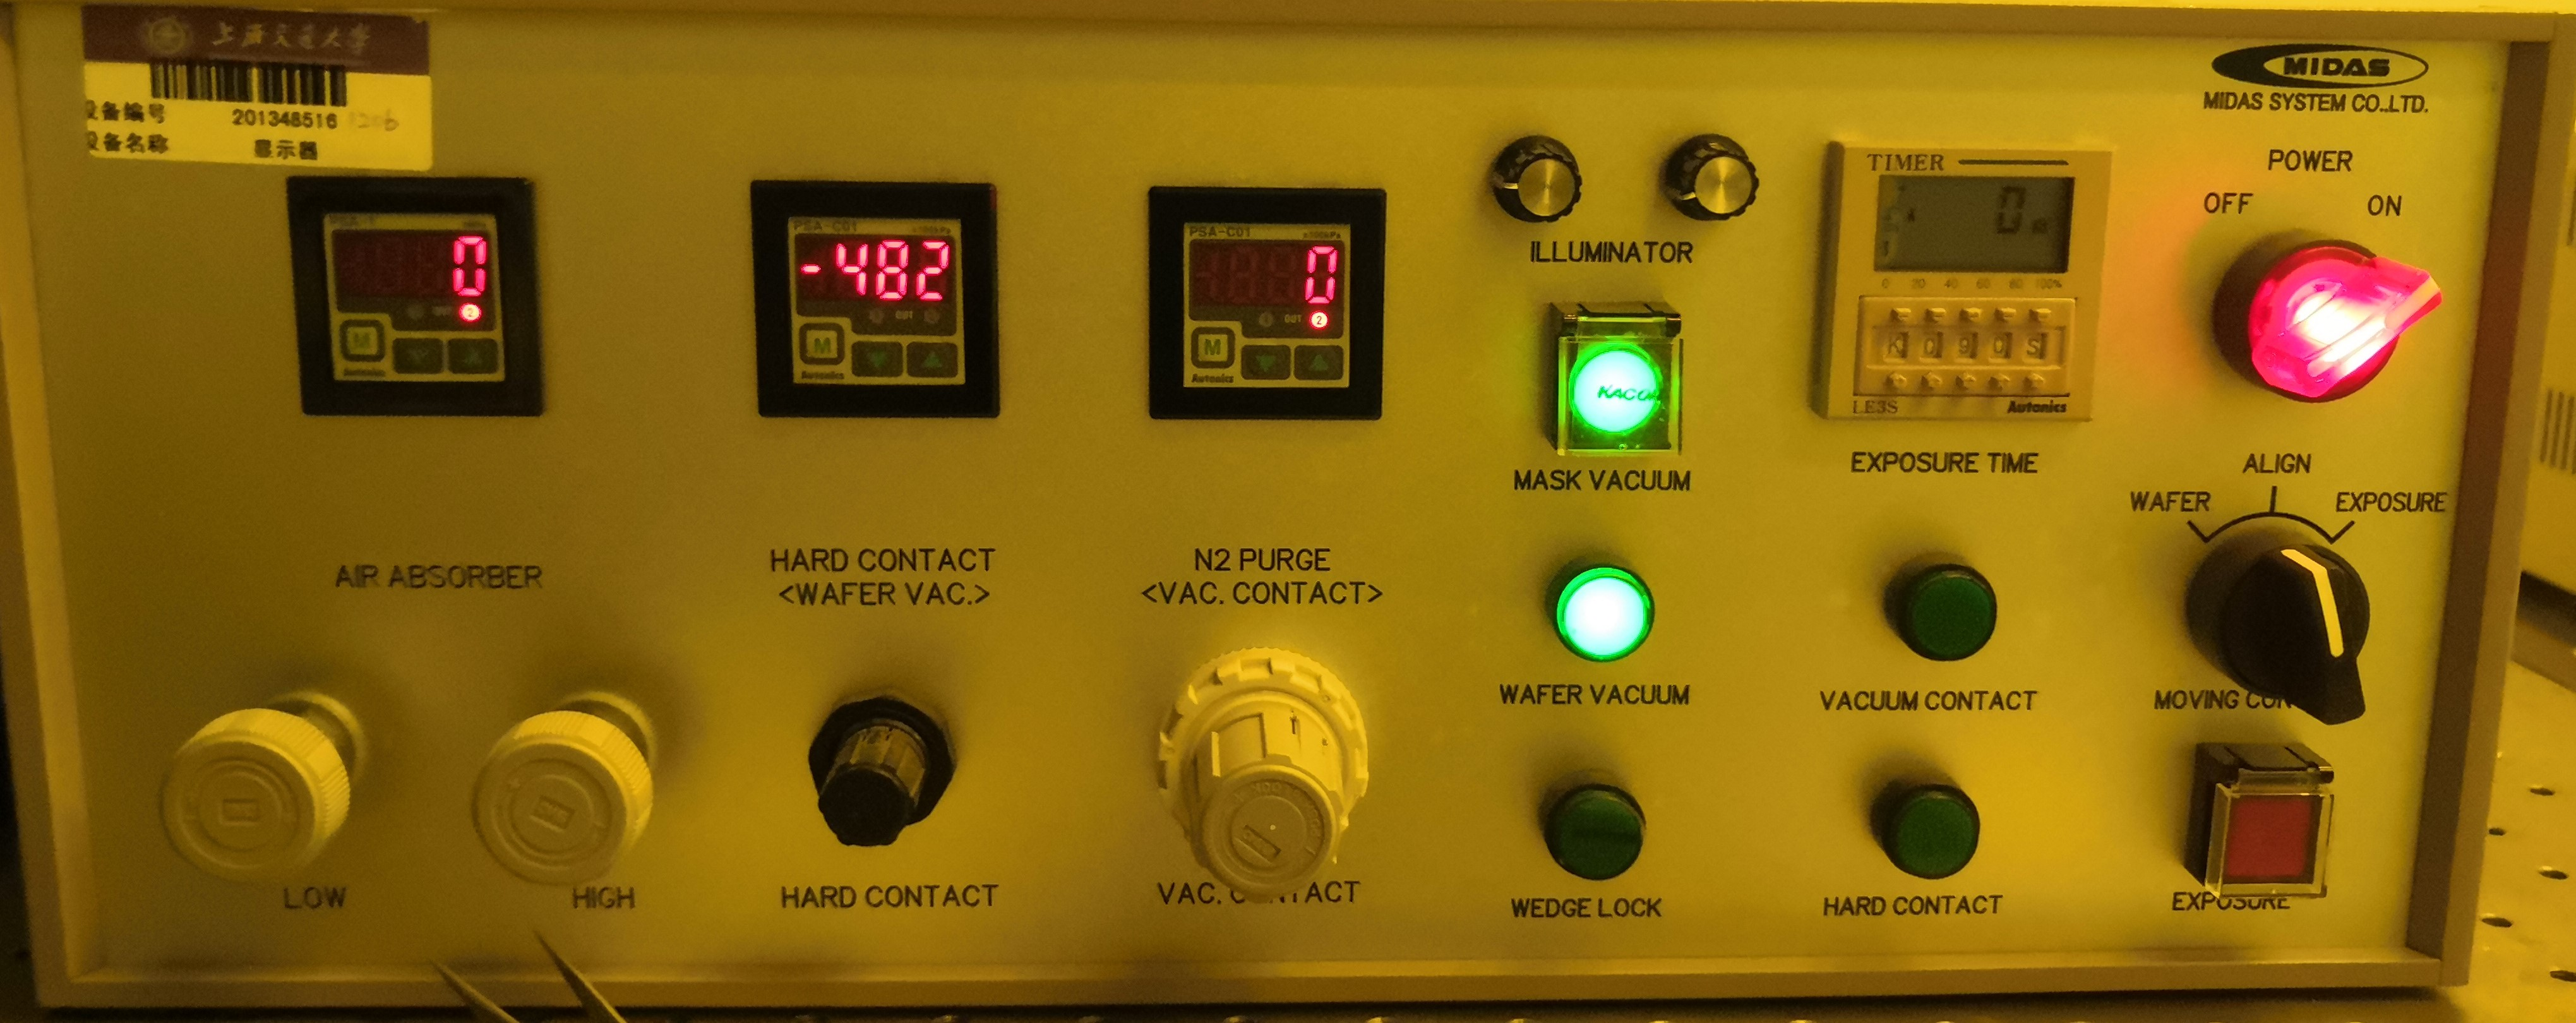
\includegraphics[width=0.365\textwidth]{EM_control_panel.jpg}}
    	\caption{The etching machine's power panel of after starting up and its control panel fixing the mask.}
    	\label{fig:etching_machine}
    \end{figure}
    \item Lithography\\
    We used the negative photoresist, NR9, for the photoetching.
        \begin{enumerate}
            \item Spinning coating\\
                The substrate was sucked in the middle of the spin coater and the speed was set to 1000 rpm for 3 s, 2000 rpm for 5 s, and 4000 rpm for 40 s. After being evenly covered by the photoresist, the spin coater would spin for 40s to make the resist uniformly attached to the substrate.
            \item Soft-bake\\
                Before photoetching, in order to remove the water in the resist and strengthen adhesion of the resist, we baked the substrate at 140$^{\circ}$C for 1 min. Then, let the substrate cool to the room temperature on the operation table.
            \item Photoetching\\
                Boot the lithography machine until the current reaches 10 A or higher. During the process, the current decays to around 4 A. To ensure the resolution of the pattern and avoid scattering of the UV light, the substrate and the mask were aligned and attached tightly together. If not, the patterns would be totally blurry (see Figure~\ref{blurry}). The exposure lasted 14s.
            \begin{figure}[H]
                \centering
                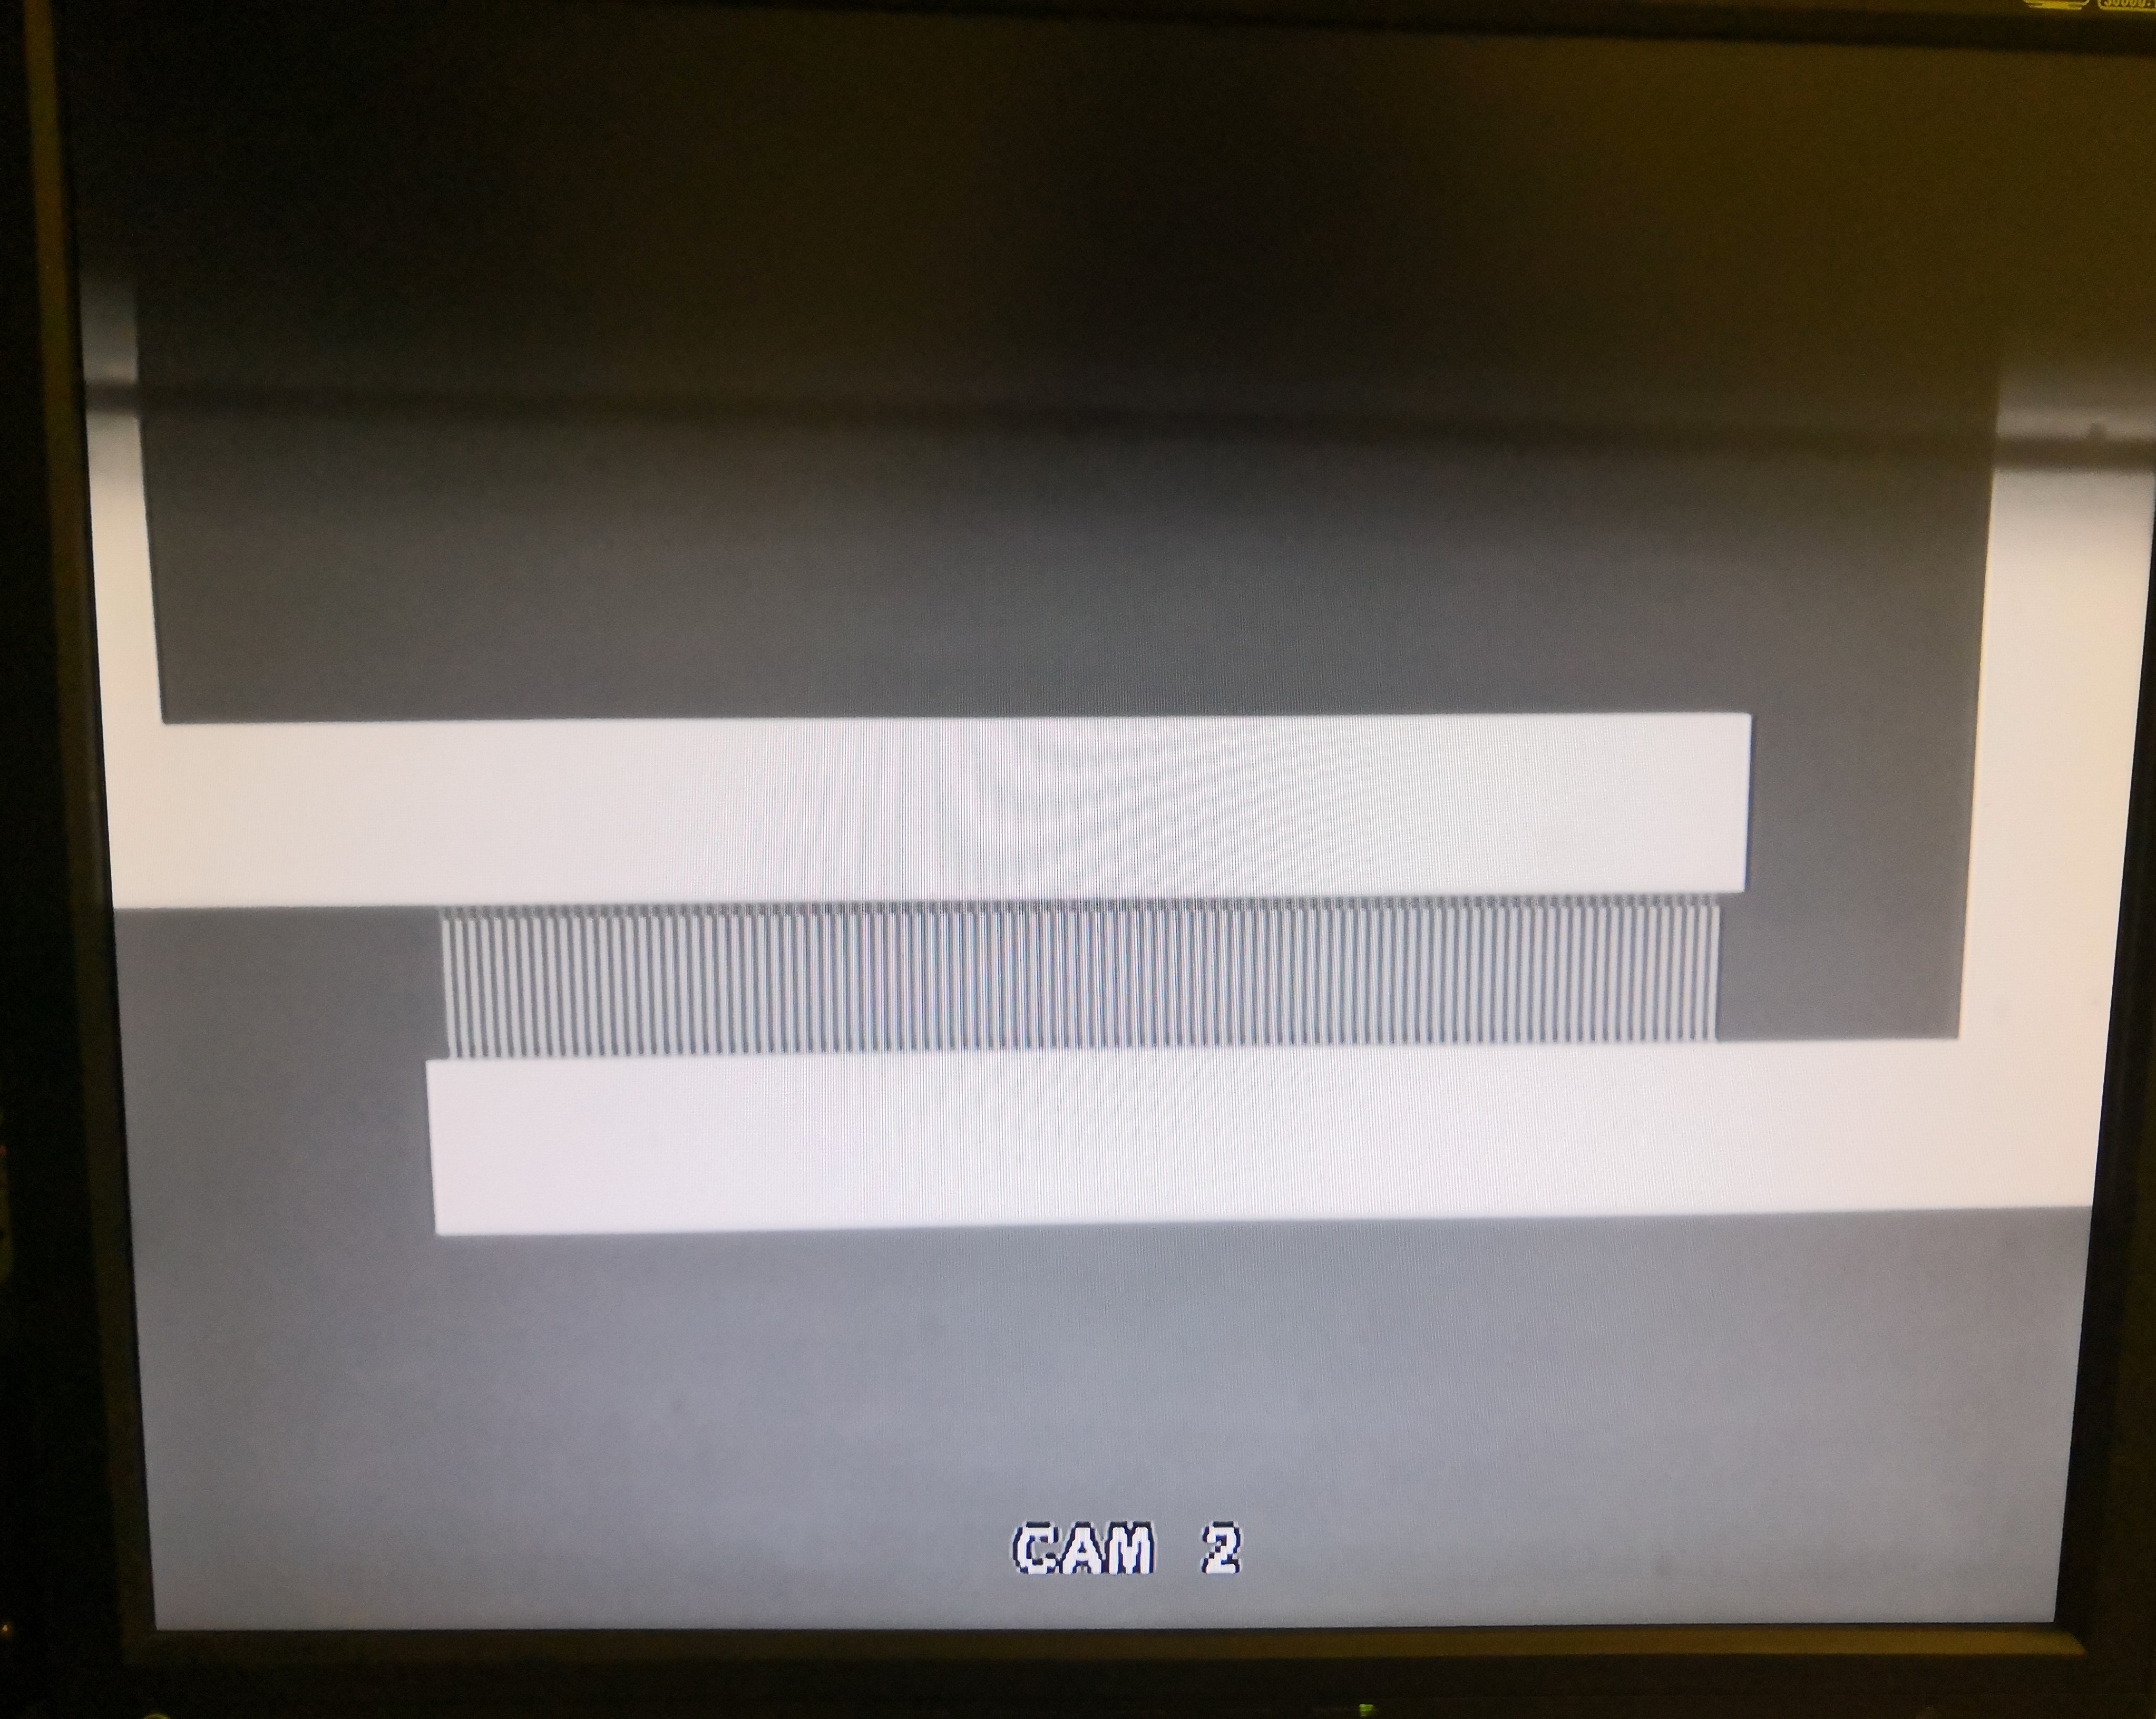
\includegraphics[width=0.5\linewidth]{EM_camera.jpg}
                \caption{Aligning the mask and the substrate using the camera of the etching machine.}
                \label{fig:EM_camera}
            \end{figure}
            \item Post-bake\\
                After exposure, the substrate was put on the hot plate to be baked at 110$^{\circ}$C for 1 min, so as to reduce the standing wave effect and make the chemical reaction more sufficient. Then, let the substrate cool to the room temperature on the operation table.
            \item Develop\\
                When the substrate was cool to the room temperature, carefully picked it up and made it immersed into the developer. Gently shook the tweezers in the developer for 8 to 10s, put it immediately into a beaker with deionized water and cleaned it for about 20s. Use the air gun to make it dry.  
            \item Observe\\
                We checked whether the electrodes patterns on the substrate had short circuit under a microscope. If it reached our expectation, it was prepared for the next step of deposition.
                In Figure~\ref{good figure}, Fig.(a) is short-circuited due to the bias of the UV light, while Fig.(b) is the expected pattern.
        \end{enumerate}
        
    \begin{figure}[H]
    	\centering
    	\subfloat[]{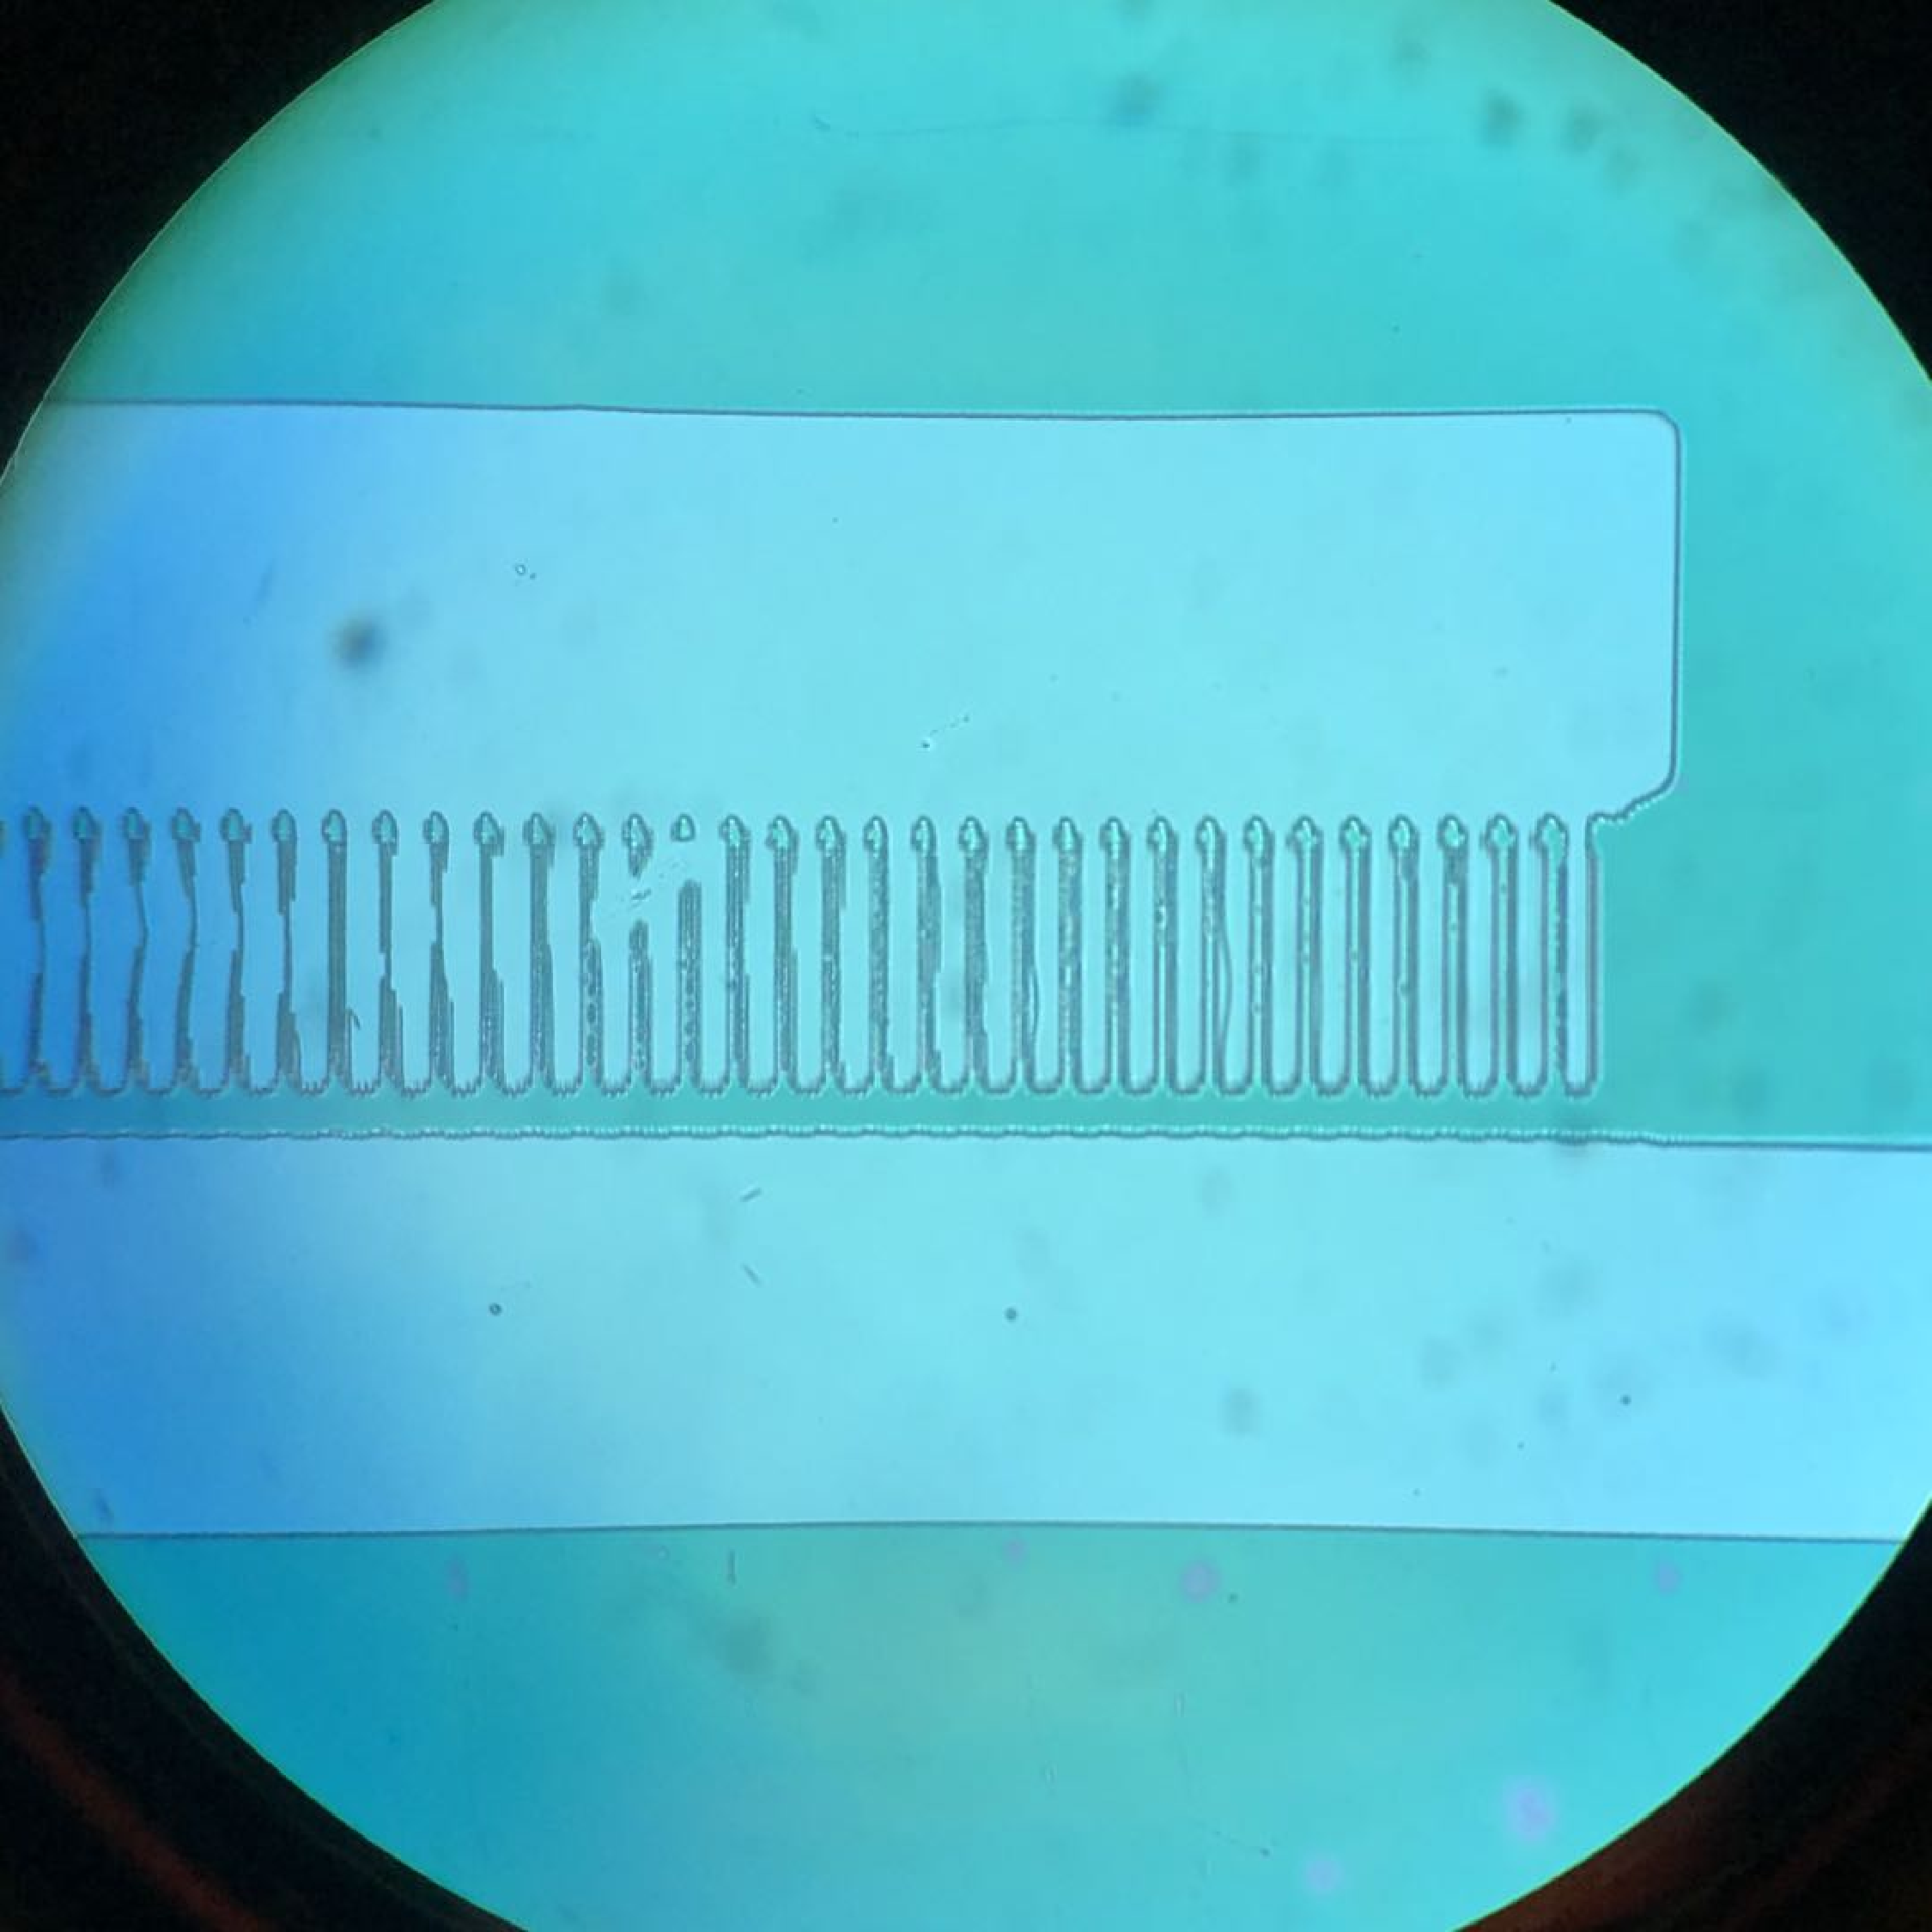
\includegraphics[width=0.3\textwidth]{blurry pattern1.pdf}}\hspace{0.4in} %% \hspace{0.8in}  insert 0.4in space between two figures
    	\subfloat[]{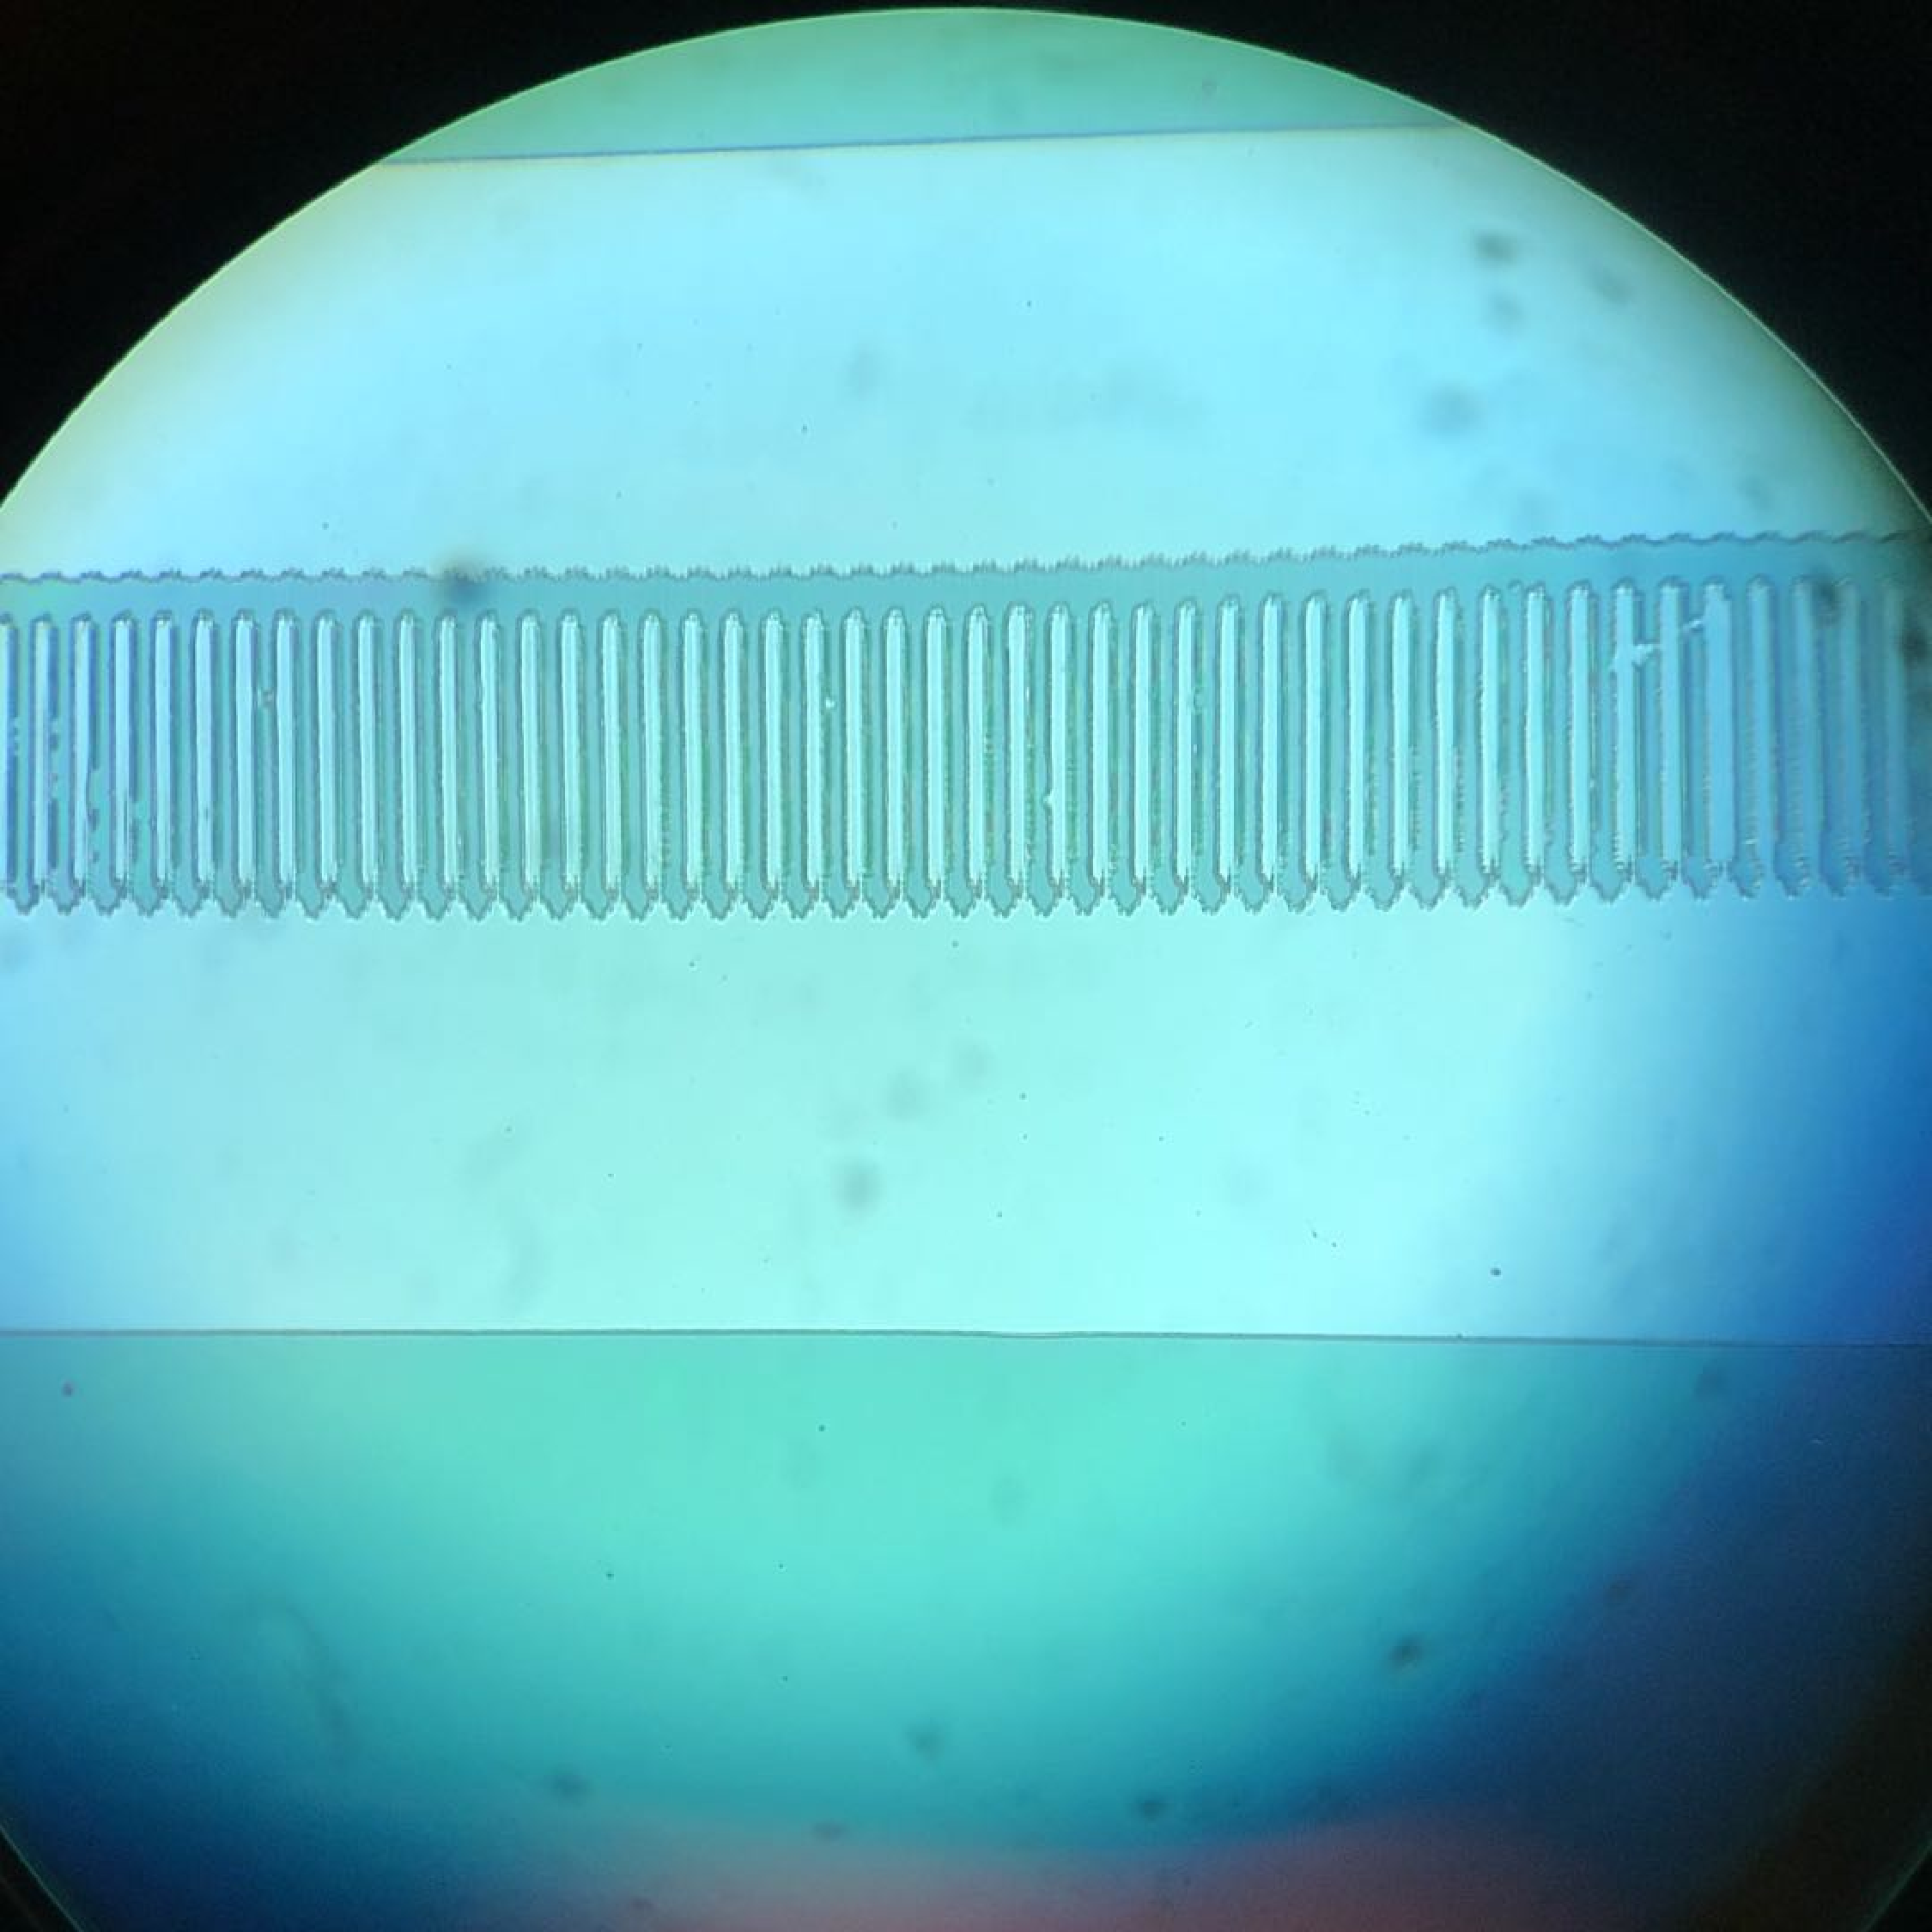
\includegraphics[width=0.3\textwidth]{blurry pattern2.pdf}}
    	\caption{Blurry photoetching patterns of the asymmetric electrodes pairs under the microscope.}
    	\label{blurry}
    \end{figure} %% one column-figure;multi column- figure*
    \begin{figure}[H]
    	\centering
    	\subfloat[Short circuit pattern.]{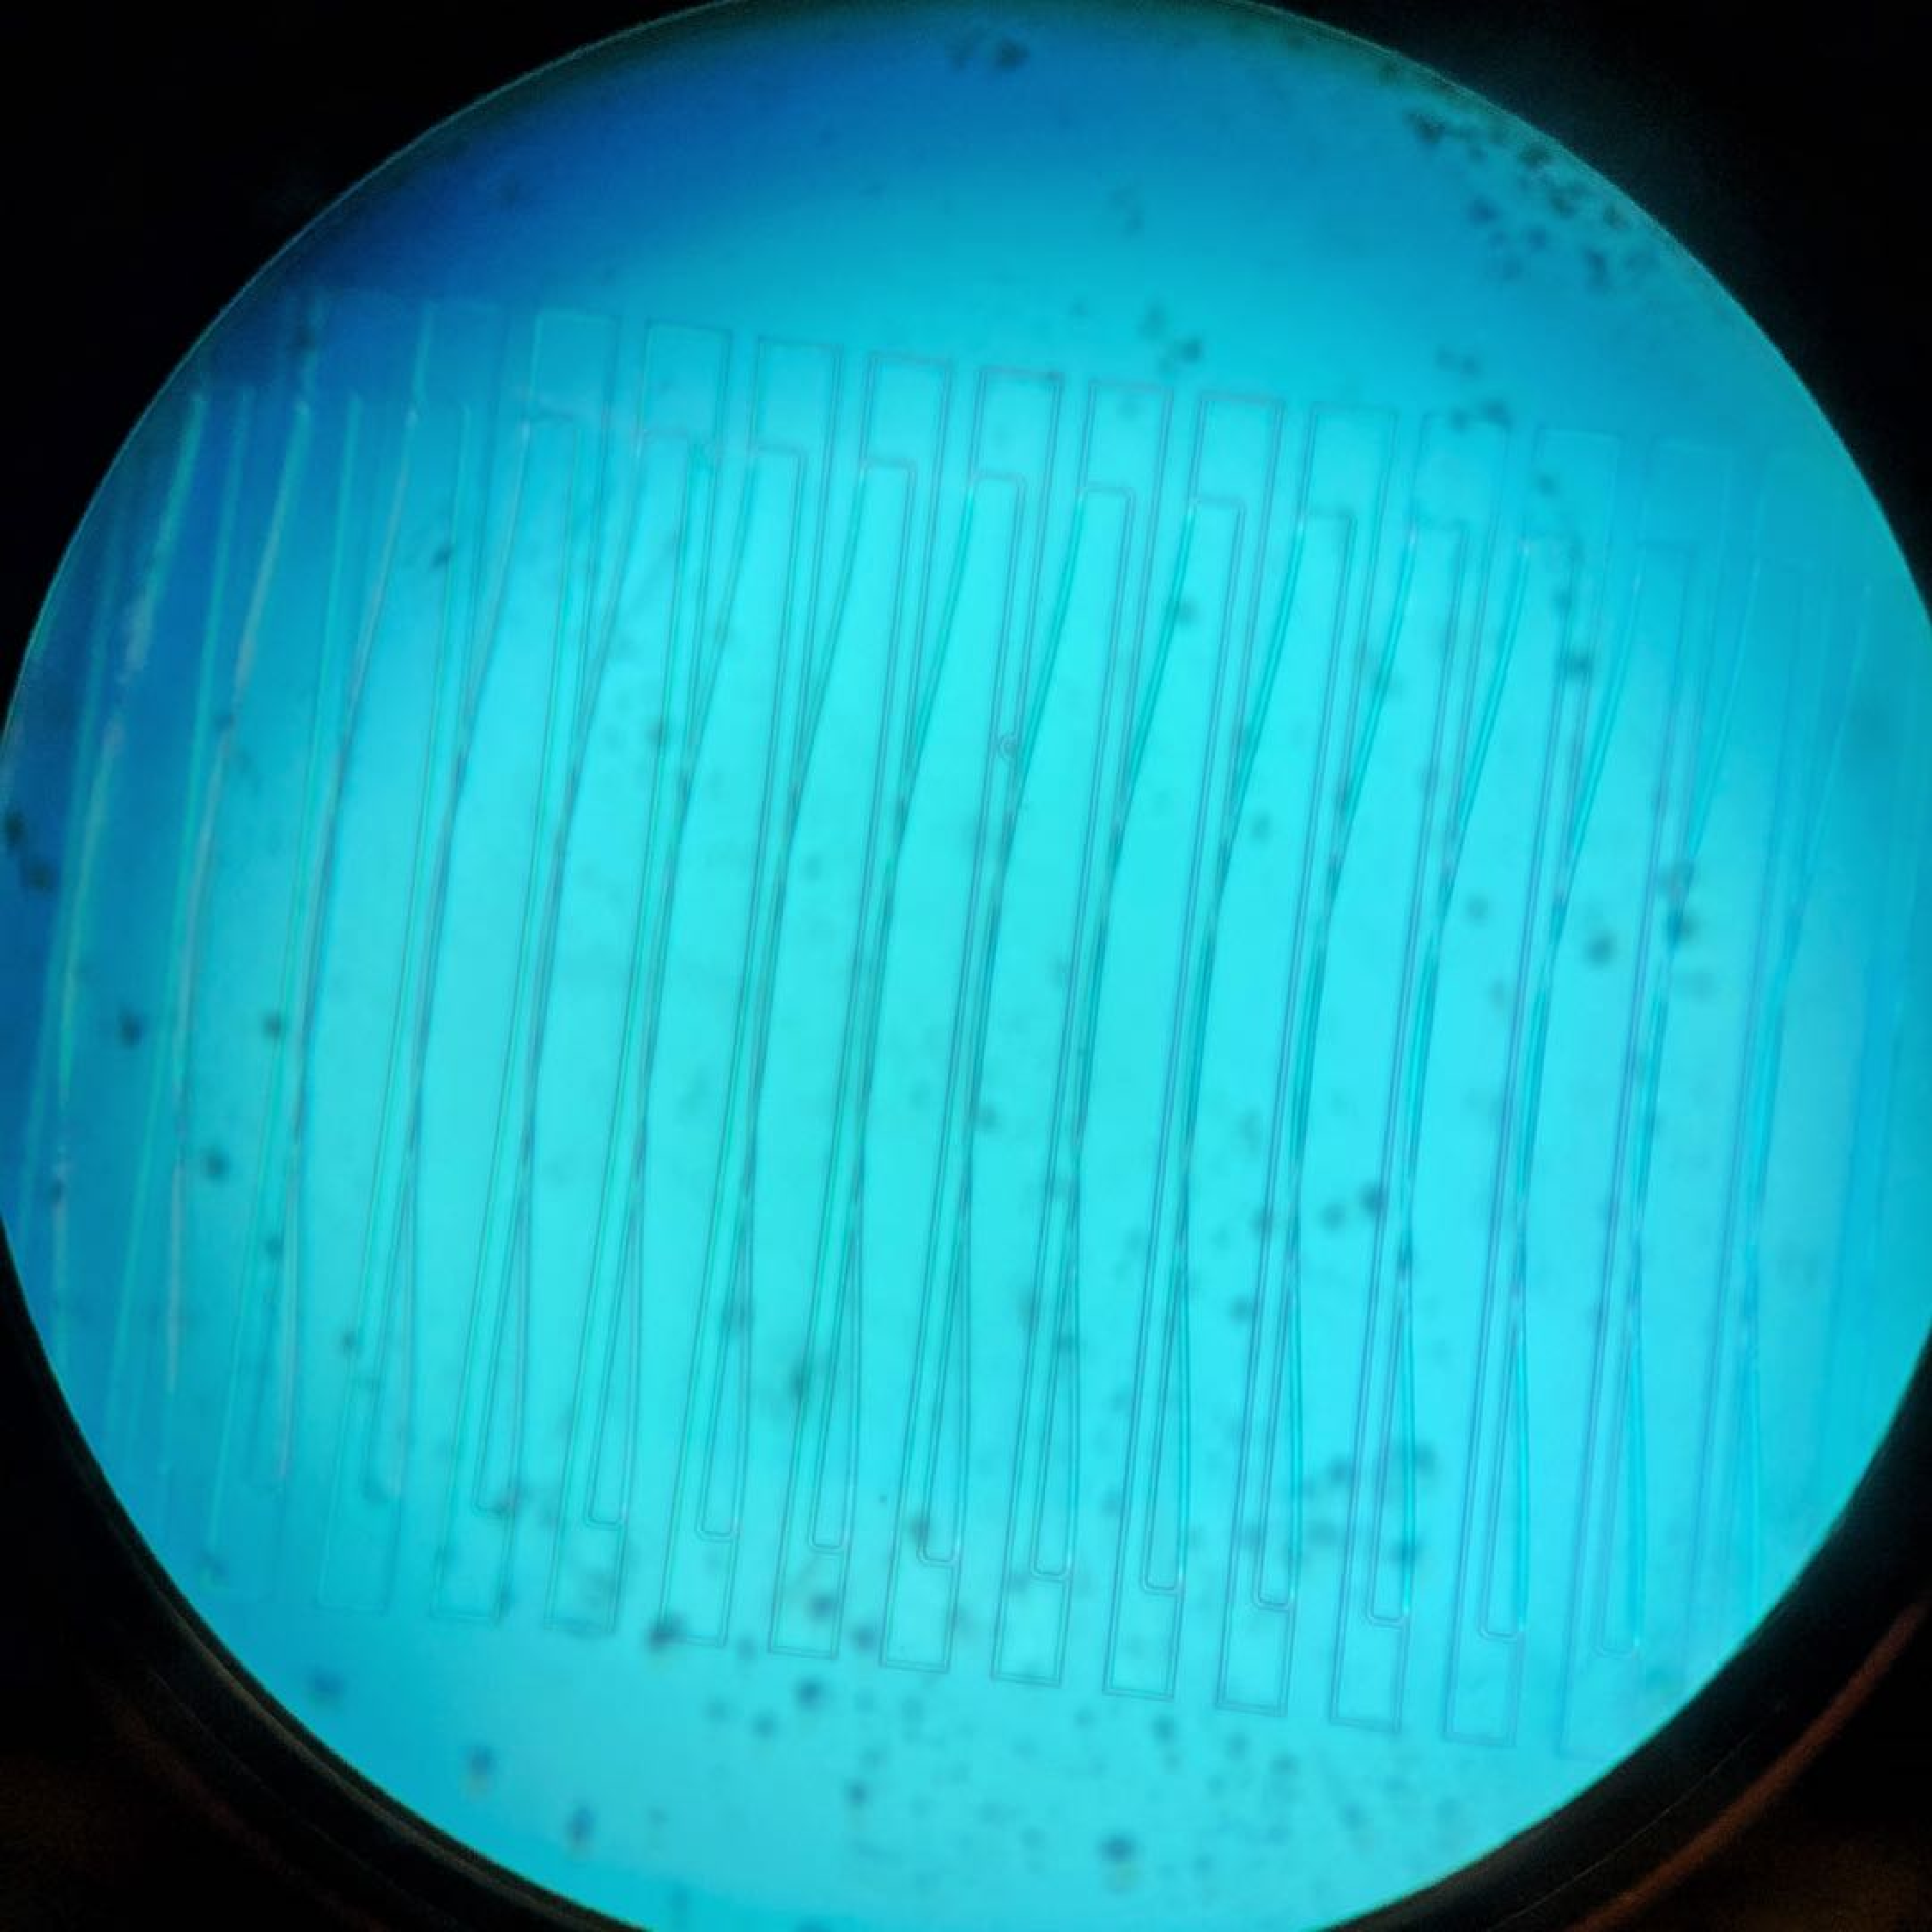
\includegraphics[width=0.3\textwidth]{short cut.pdf}}\hspace{0.4in} %% \hspace{0.8in}  insert 0.4in space between two figures
    	\subfloat[Perfect pattern.]{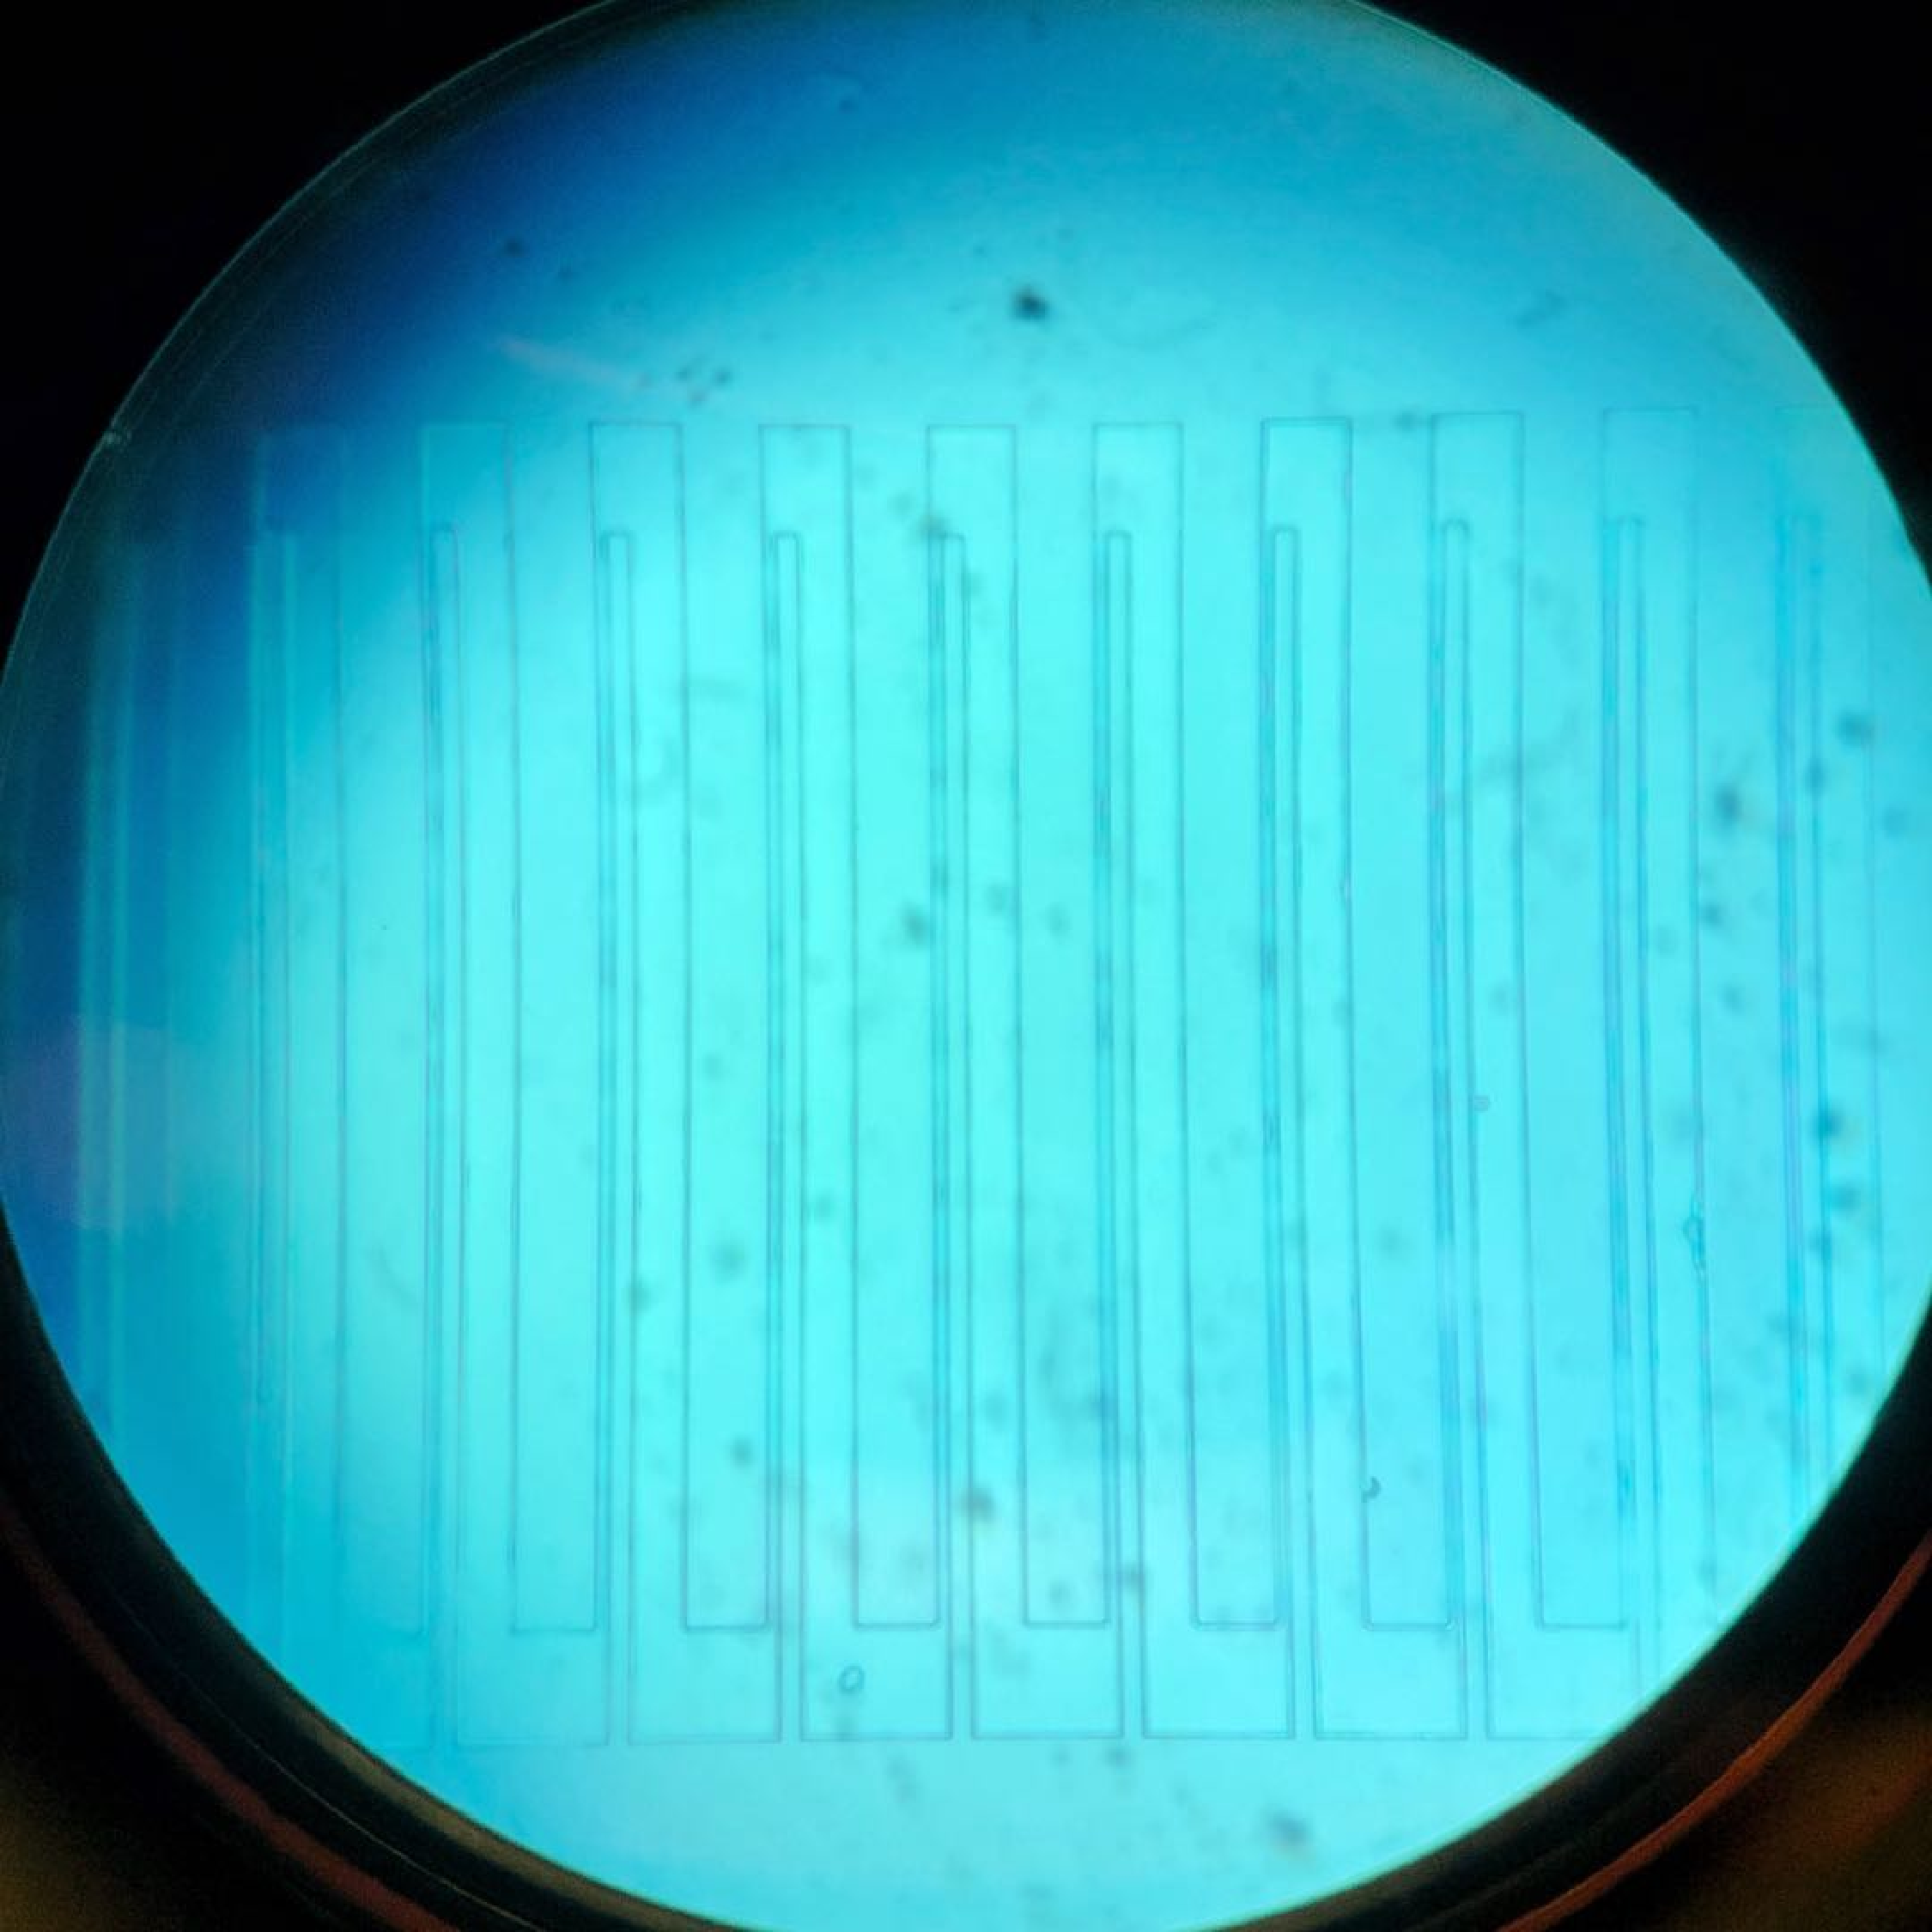
\includegraphics[width=0.3\textwidth]{good pattern.pdf}}
    	\caption{Different results of the photoetching.}
    	\label{good figure}
    \end{figure} %% one column-figure;multi column- figure*
    
    \item Deposition and Lift-off
    \\
        \begin{enumerate}
            \item Check and open the nitrogen container.
            \item Open the cold water circulator and wait for 180 s.
            \item Switch the mode to "front". Pull the “EMERGENCY STOP” button out. The red pilot lamp is then off. Turn on the pump for 5 s and turn off.
            \item Slightly open the buckle of the door of the cabin and wait for vacuum relieving, because the high speed gas stream at the moment the door opens is dangerous. After the inner pressure is high enough, the door will automatically open.
            \item After the door of the cabin opens, take out the sample plate and put it on the a clean paper on the desk. Then, label the sample. Use air blower to clean the inner cavity of the cabin.
            \item Fix the metal boats on their corresponding locations. Conventionally, the pocket 1 is for the gold boat and the pocket 3 is for the aluminium boat. Add appropriate amount of plating material. Do not change the convention, otherwise the metal will not be pure.
            \item Put the sample in the cabin.
            \item Use a multimeter to examine whether there is a short circuit between the electrode and the inner metal shell of the cabin for each of the pockets at the corresponding places.
            \item If there are not any short circuits, close the door of the cabin and quickly press the buckle from top to bottom.
            
            \begin{figure}[H]
            	\centering
            	\subfloat[Control panel.]{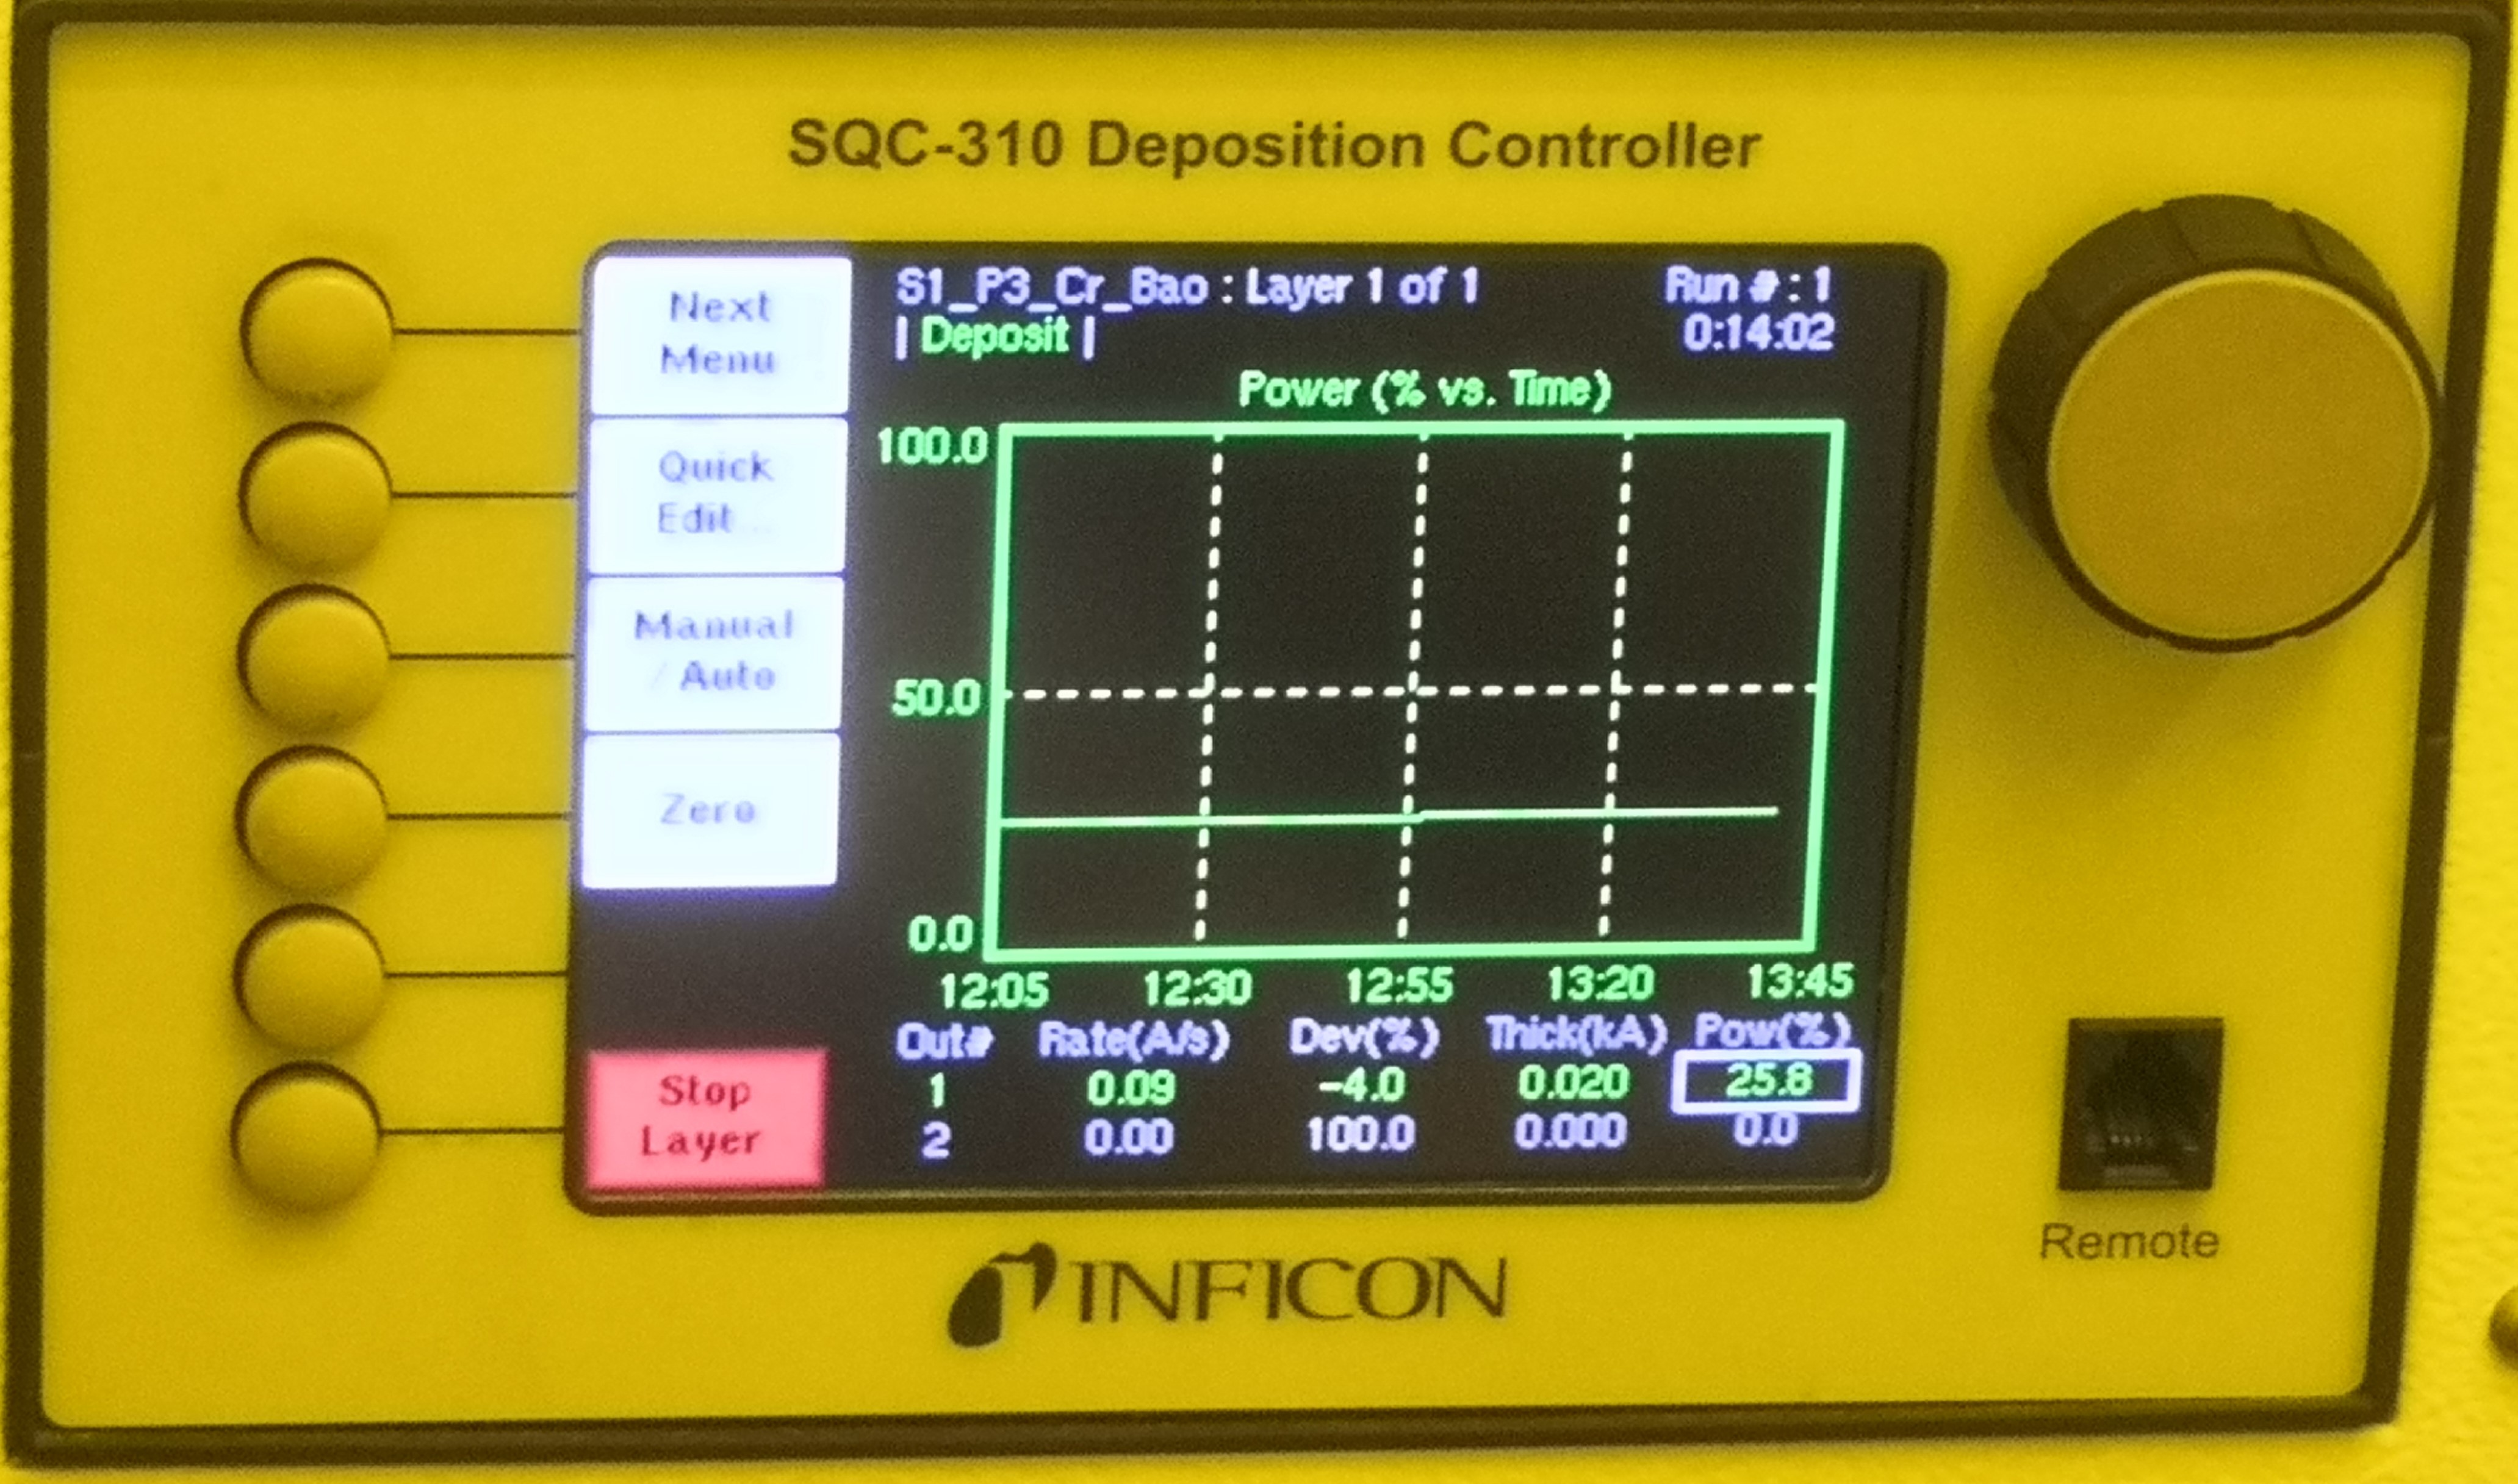
\includegraphics[width=0.44\textwidth]{control_panel.jpg}}\hspace{0.4in}
            	\subfloat[Deposition.]{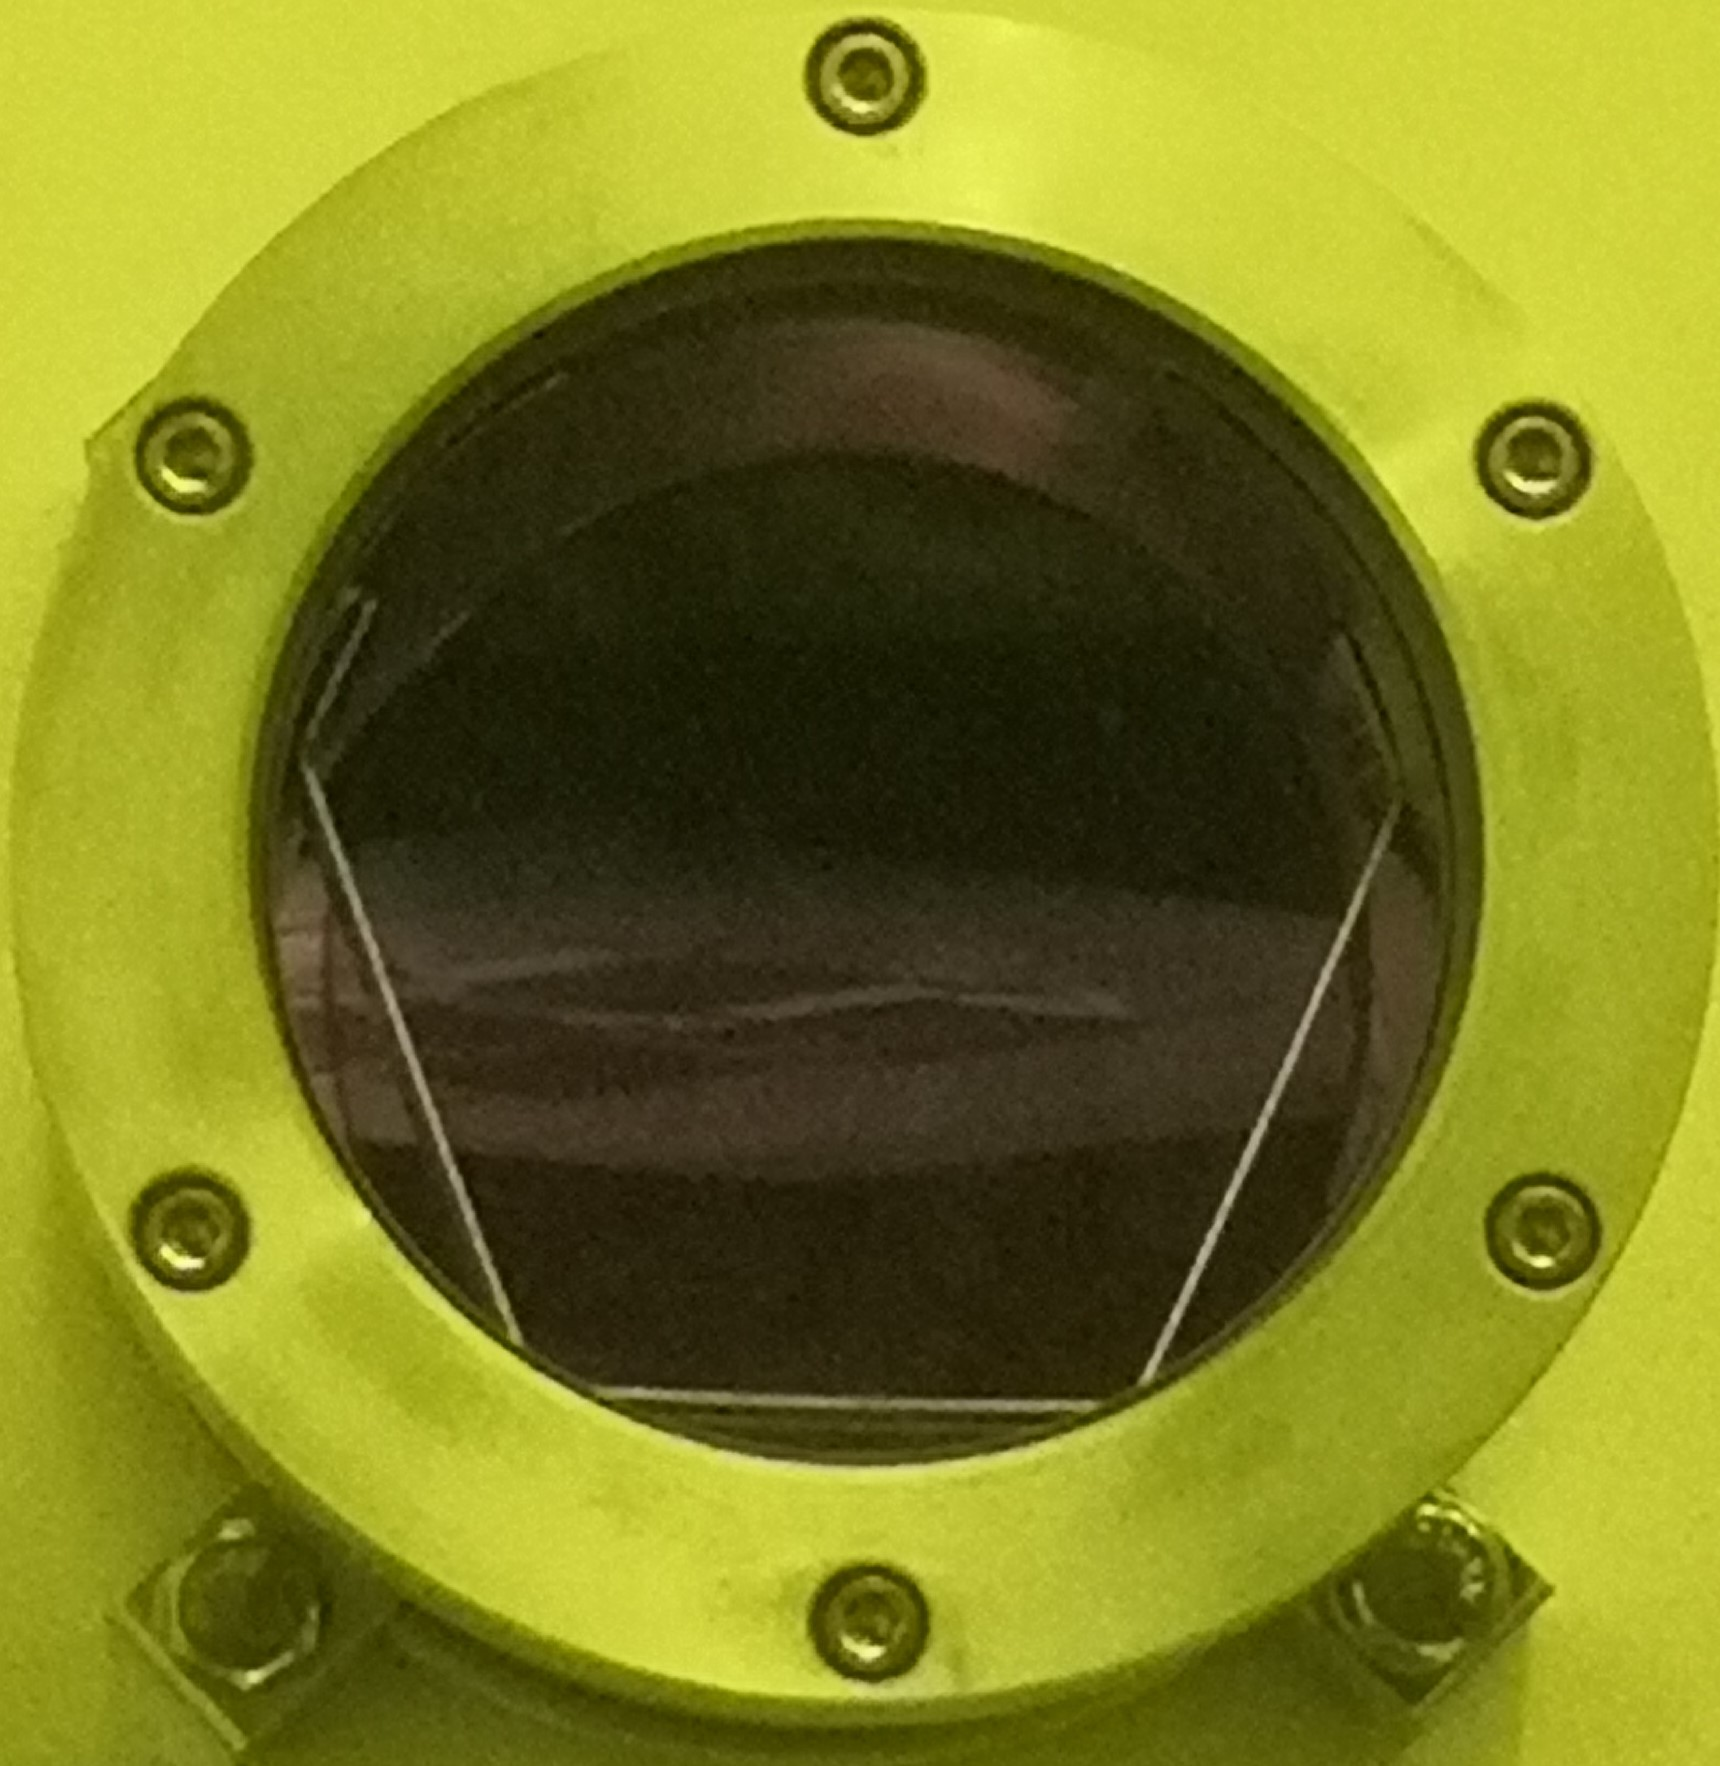
\includegraphics[width=0.25\textwidth]{deposit.jpg}}
            	\caption{The control panel of the deposition machine when depositing chromium. The deposit rate is $0.09\,\mathrm{\AA/s}$ and the thickness of the chromium is $0.020\,\mathrm{k\AA}$.}
                \label{fig:control_panel}
            \end{figure}
            
            \item Switch the mode to "remote". Turn on the pump. Wait until the frequency of the molecular pump reaches "normal" as shown in the control panel.
            \item When the vacuum degree inside the cabin reaches $5\times10^{-6}$ Torr (the vacuumization requires approximately 2 hours), select and start the program for plating aluminium or chromium. For plating gold, for the sake of conservation, the pressure should be less than $5\times10^{-6}$ Torr. Switch the mode to "manual", slowly rotate the knob to adjust frequency so that the deposit rate stabilize at around $0.10\,\mathrm{\AA/s}$.
            \item After the deposit process finishes, wait for 15 minutes and close the pump. Still, slightly open the buckle of the door of the cabin and wait for vacuum relieving.
            \item Take off the sample board, take off the sample and put back the sample board. Clean the inner cavity of the cabin.
            \item Close the door of the cabin, switch the mode back to "front", and close the pump when the inner pressure drops to $10^{-2}$ Torr.
            \item Close the cold water circulator. Close the high-purity nitrogen gas (99.9999\%) and ordinary nitrogen gas (99.99\%).
            \item Lift-off\\
                Use clean adequate acetone to soak the substrate for 12 hours and then wash off the metal with a dropper carefully.
        \end{enumerate}
\end{enumerate}

\begin{figure}[H]
    \centering
    \subfloat[After deposition.]{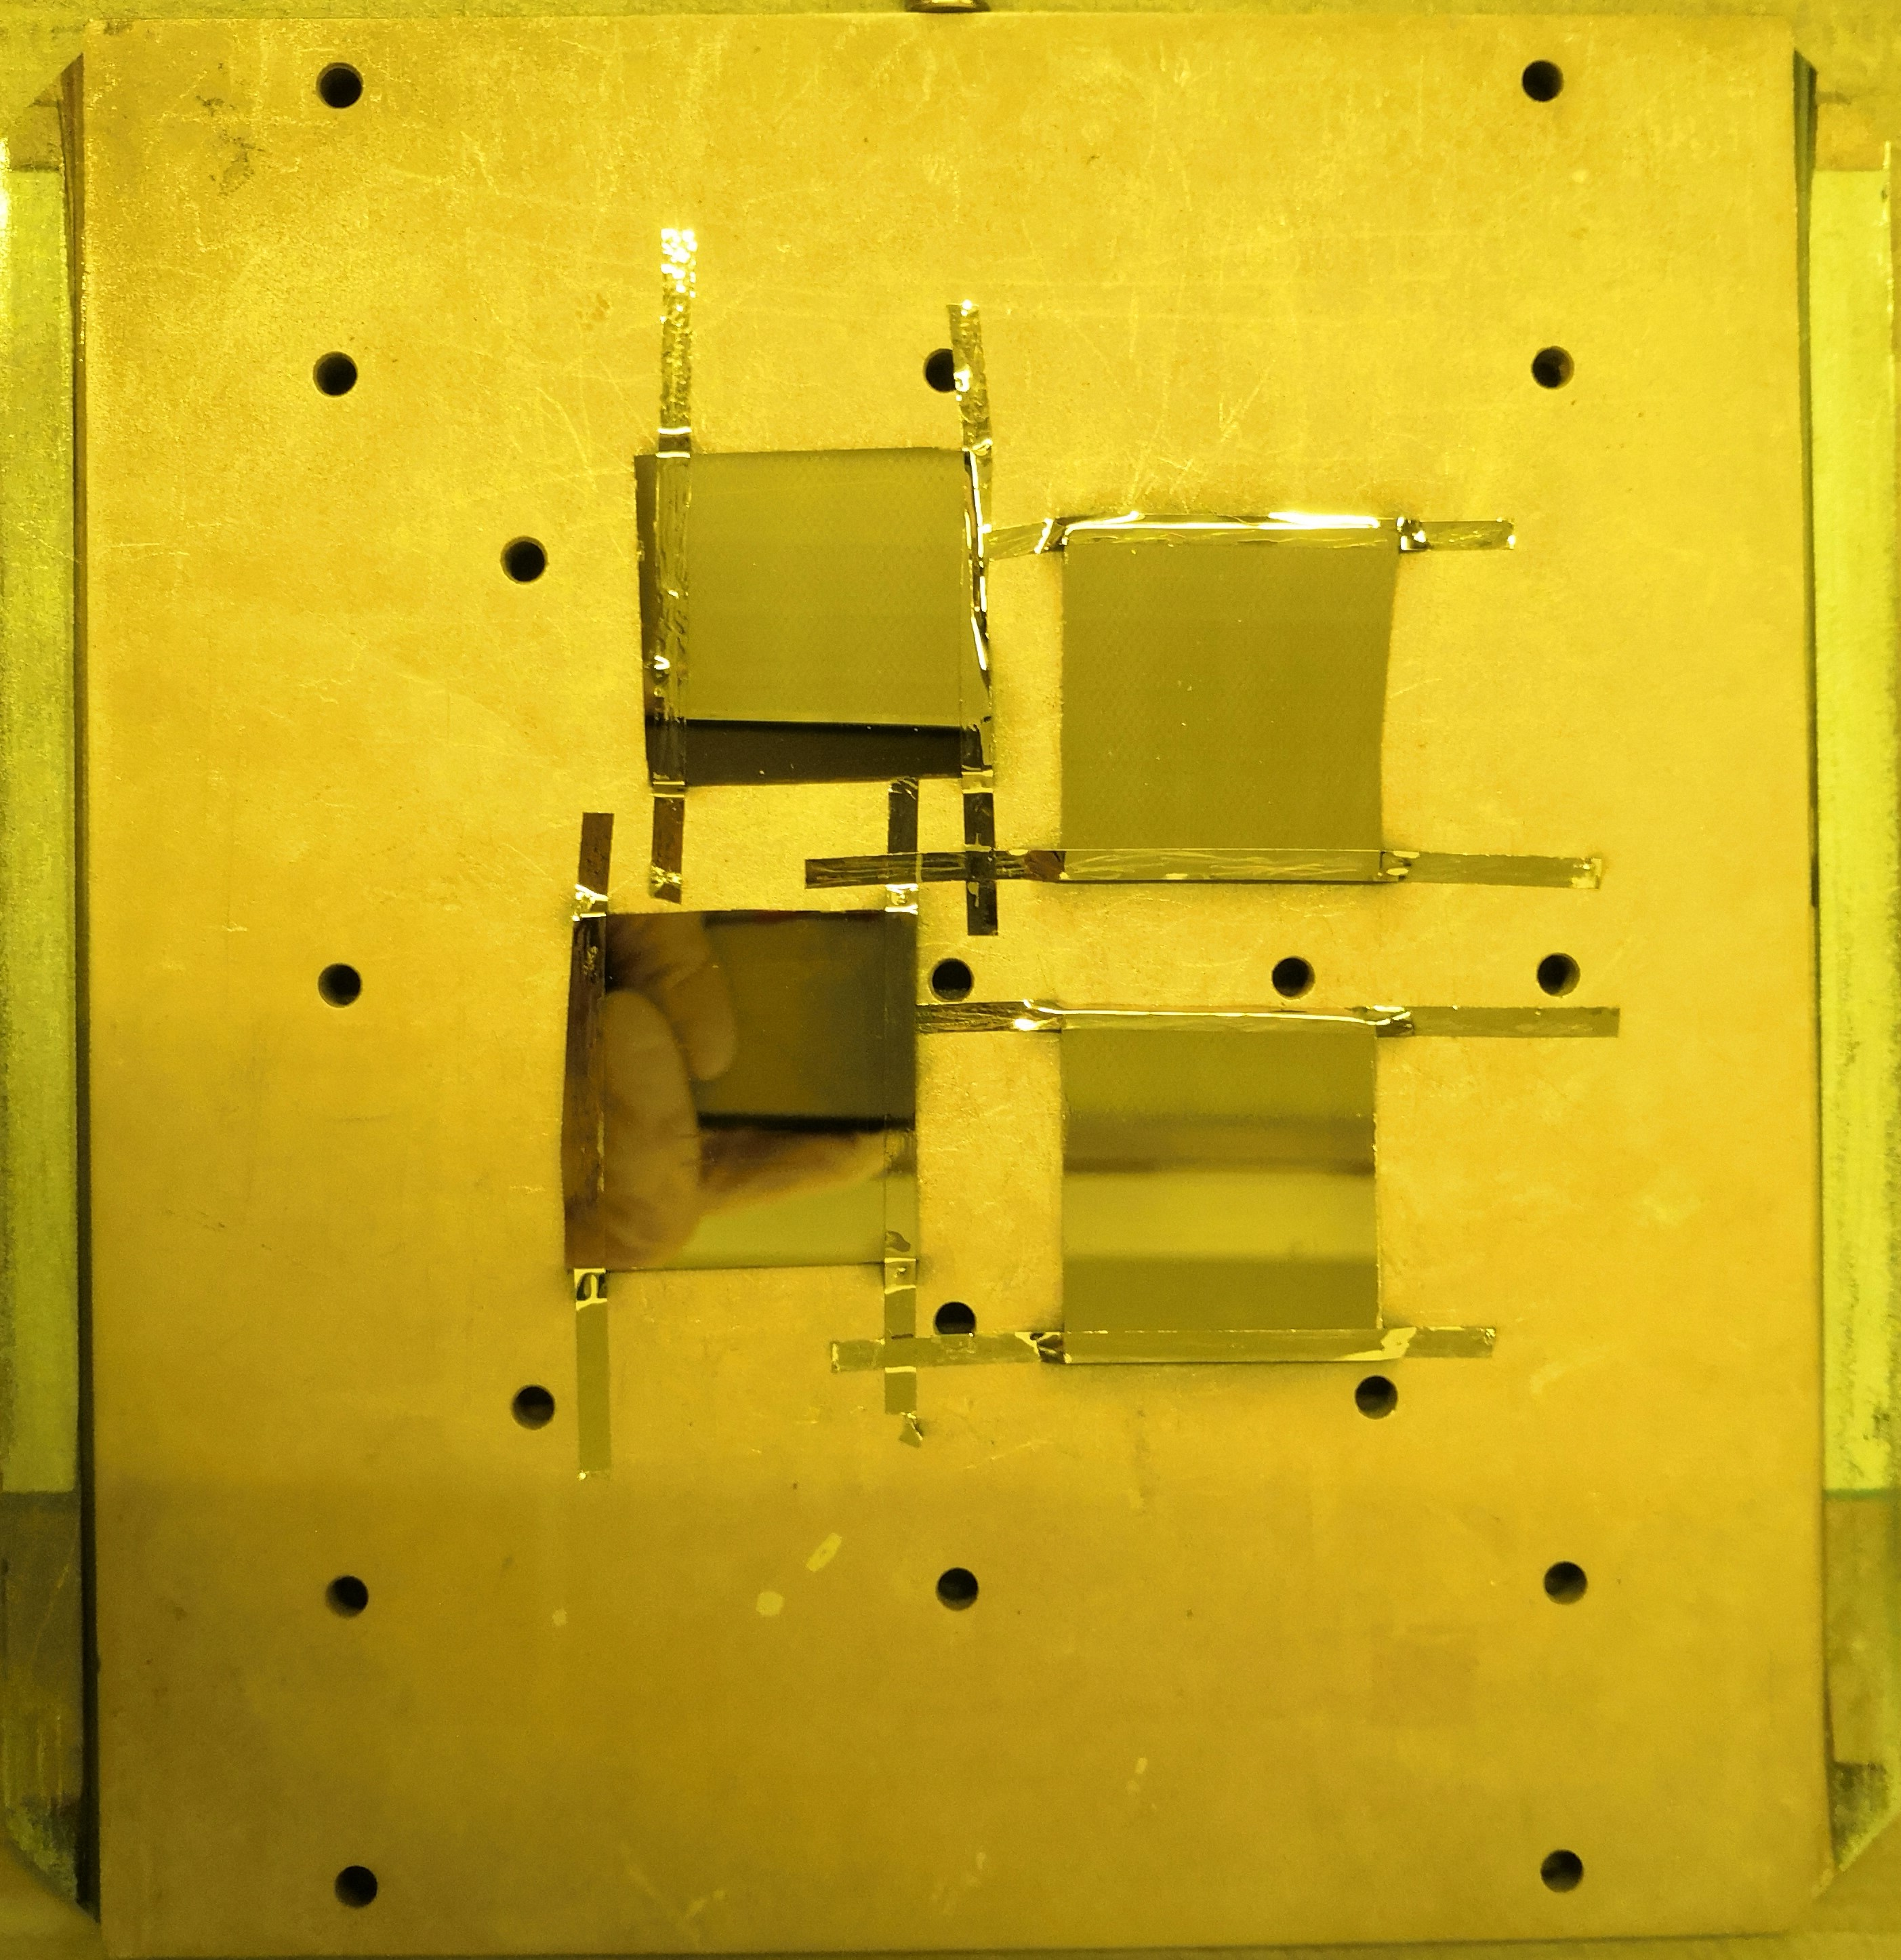
\includegraphics[width=0.245\textwidth]{gold_board_1.jpg}}
    \hspace{0.2in}
	\subfloat[Lift-off.]{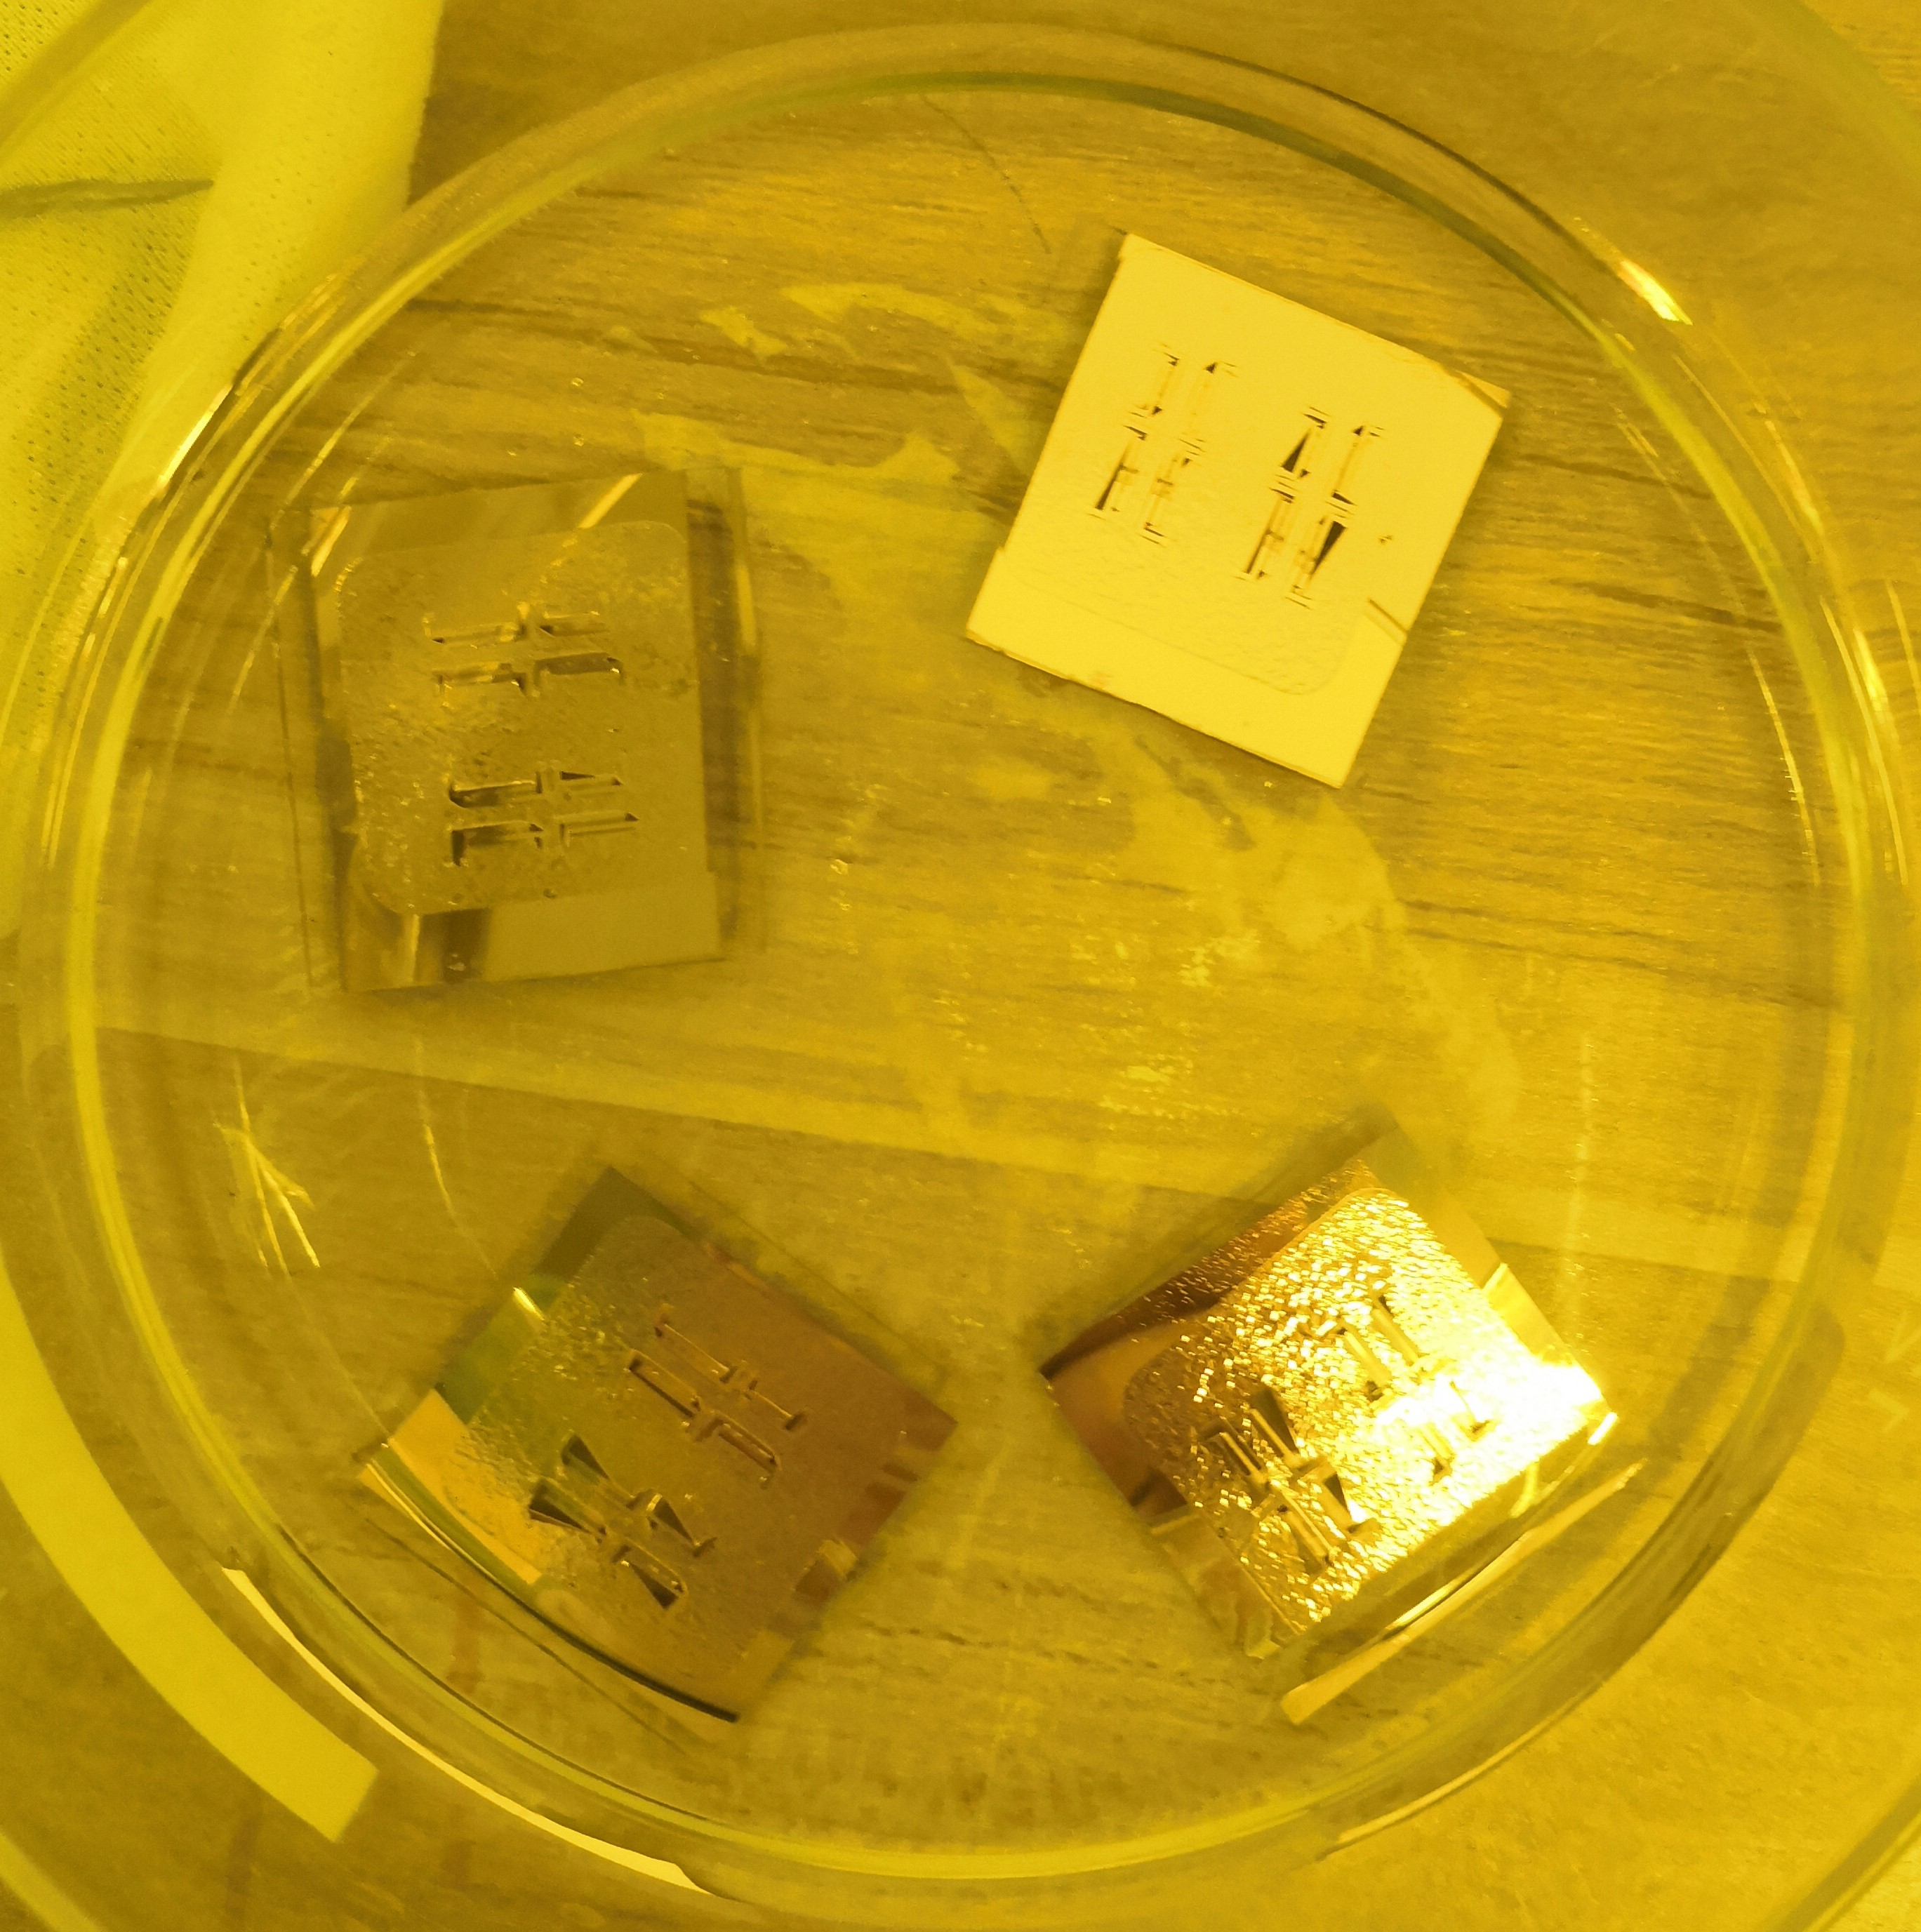
\includegraphics[width=0.25\textwidth]{gold_board_2.jpg}}
	\hspace{0.2in}
	%\\
	\subfloat[After lift-off.]{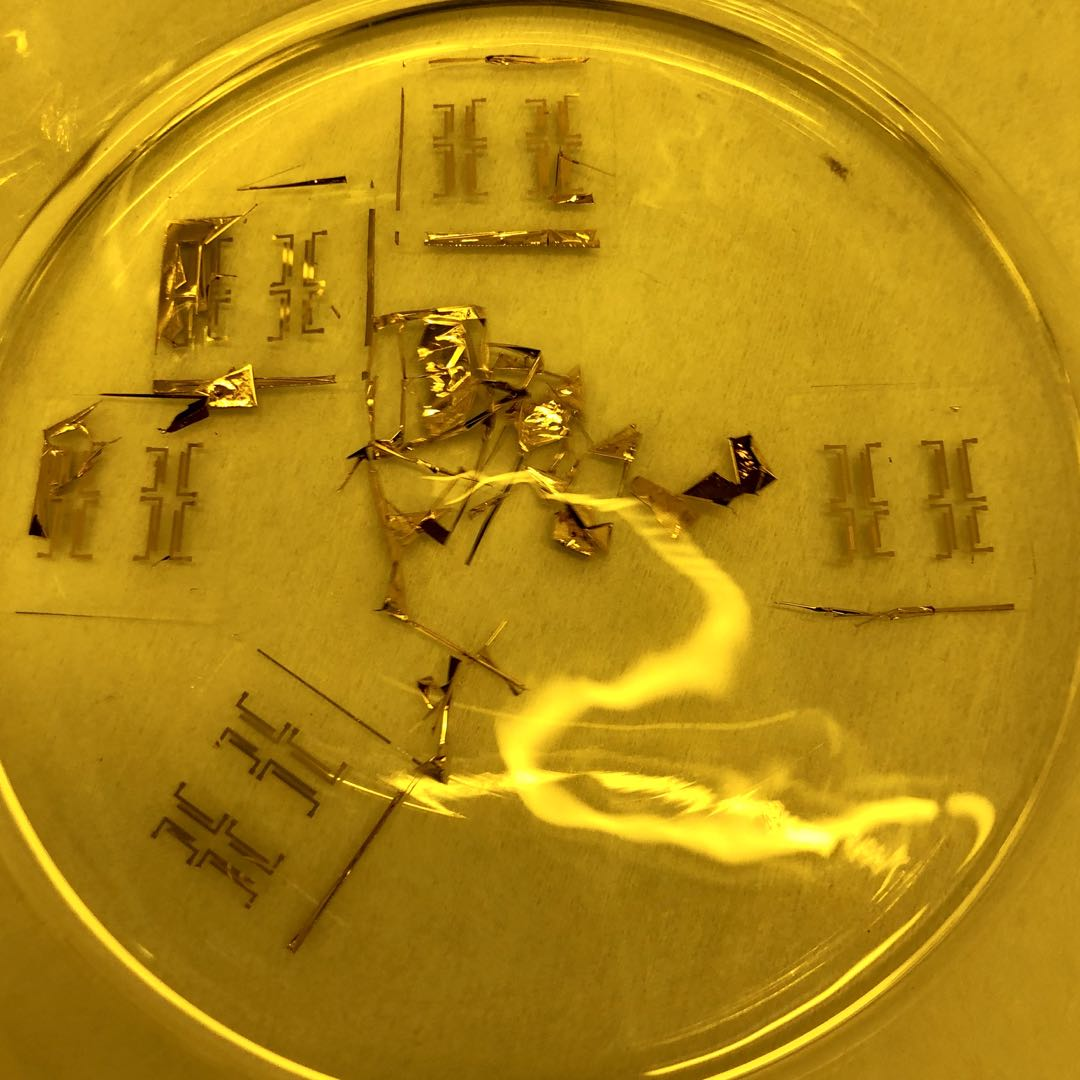
\includegraphics[width=0.25\textwidth]{lift_off.jpg}}
    \caption{The electrode plate after deposition.}
    \label{fig:gold_board}
\end{figure}
\end{document}

